\documentclass{book}
\usepackage[a4paper,top=2.5cm,bottom=2.5cm,left=2.5cm,right=2.5cm]{geometry}
\usepackage{makeidx}
\usepackage{natbib}
\usepackage{graphicx}
\usepackage{multicol}
\usepackage{float}
\usepackage{listings}
\usepackage{color}
\usepackage{ifthen}
\usepackage[table]{xcolor}
\usepackage{textcomp}
\usepackage{alltt}
\usepackage{ifpdf}
\ifpdf
\usepackage[pdftex,
            pagebackref=true,
            colorlinks=true,
            linkcolor=blue,
            unicode
           ]{hyperref}
\else
\usepackage[ps2pdf,
            pagebackref=true,
            colorlinks=true,
            linkcolor=blue,
            unicode
           ]{hyperref}
\usepackage{pspicture}
\fi
\usepackage[utf8]{inputenc}
\usepackage{mathptmx}
\usepackage[scaled=.90]{helvet}
\usepackage{courier}
\usepackage{sectsty}
\usepackage[titles]{tocloft}
\usepackage{doxygen}
\lstset{language=C++,inputencoding=utf8,basicstyle=\footnotesize,breaklines=true,breakatwhitespace=true,tabsize=4,numbers=left }
\makeindex
\setcounter{tocdepth}{3}
\renewcommand{\footrulewidth}{0.4pt}
\renewcommand{\familydefault}{\sfdefault}
\hfuzz=15pt
\setlength{\emergencystretch}{15pt}
\hbadness=750
\tolerance=750
\begin{document}
\hypersetup{pageanchor=false,citecolor=blue}
\begin{titlepage}
\vspace*{7cm}
\begin{center}
{\Large K\-Utils }\\
\vspace*{1cm}
{\large Generated by Doxygen 1.8.0}\\
\vspace*{0.5cm}
{\small Mon May 7 2012 13:25:06}\\
\end{center}
\end{titlepage}
\clearemptydoublepage
\pagenumbering{roman}
\tableofcontents
\clearemptydoublepage
\pagenumbering{arabic}
\hypersetup{pageanchor=true,citecolor=blue}
\chapter{Namespace Index}
\section{Namespace List}
Here is a list of all namespaces with brief descriptions\-:\begin{DoxyCompactList}
\item\contentsline{section}{\hyperlink{namespaceargparse}{argparse} \\*Command-\/line argument parser with a focus on brevity }{\pageref{namespaceargparse}}{}
\item\contentsline{section}{\hyperlink{namespaceautodiff}{autodiff} \\*Implements automatic differentiation }{\pageref{namespaceautodiff}}{}
\item\contentsline{section}{\hyperlink{namespacecvutils}{cvutils} \\*Open\-C\-V utilities }{\pageref{namespacecvutils}}{}
\item\contentsline{section}{\hyperlink{namespacecvutils_1_1geom}{cvutils\-::geom} \\*Operations on {\ttfamily cv\-::\-Point}s, {\ttfamily cv\-::\-Vec}s, and {\ttfamily cv\-::\-Rect}s }{\pageref{namespacecvutils_1_1geom}}{}
\item\contentsline{section}{\hyperlink{namespacecvutils_1_1transform}{cvutils\-::transform} \\*Functions related to affine transformations }{\pageref{namespacecvutils_1_1transform}}{}
\item\contentsline{section}{\hyperlink{namespacedict}{dict} \\*Utilities for working with {\ttfamily Dict}s ({\ttfamily unordered\-\_\-map}s) }{\pageref{namespacedict}}{}
\item\contentsline{section}{\hyperlink{namespacehumancv}{humancv} \\*Human-\/related computer vision utilities }{\pageref{namespacehumancv}}{}
\item\contentsline{section}{\hyperlink{namespacehumancv_1_1face}{humancv\-::face} \\*Basic face detection and modeling }{\pageref{namespacehumancv_1_1face}}{}
\item\contentsline{section}{\hyperlink{namespacehumancv_1_1skin}{humancv\-::skin} \\*Color-\/based skin segmentation }{\pageref{namespacehumancv_1_1skin}}{}
\item\contentsline{section}{\hyperlink{namespaceio}{io} \\*Convenience functions for printing values }{\pageref{namespaceio}}{}
\item\contentsline{section}{\hyperlink{namespacekmath}{kmath} \\*Miscellaneous mathematical functions }{\pageref{namespacekmath}}{}
\item\contentsline{section}{\hyperlink{namespacekrandom}{krandom} \\*Simple wrapper around {\ttfamily $<$random$>$} with a Python-\/like interface }{\pageref{namespacekrandom}}{}
\item\contentsline{section}{\hyperlink{namespacektime}{ktime} \\*Utilities for working with time }{\pageref{namespacektime}}{}
\item\contentsline{section}{\hyperlink{namespacemouse}{mouse} \\*Utilities for modeling the mouse state }{\pageref{namespacemouse}}{}
\item\contentsline{section}{\hyperlink{namespaceosx}{osx} \\*O\-S\-X-\/specific utilities }{\pageref{namespaceosx}}{}
\item\contentsline{section}{\hyperlink{namespaceosx_1_1disp}{osx\-::disp} \\*Functions for extracting the display image }{\pageref{namespaceosx_1_1disp}}{}
\item\contentsline{section}{\hyperlink{namespaceosx_1_1mouse}{osx\-::mouse} \\*Utilities for modeling the mouse state and controlling the mouse }{\pageref{namespaceosx_1_1mouse}}{}
\item\contentsline{section}{\hyperlink{namespaceosx__cv}{osx\-\_\-cv} \\*Functions for interoperability between Application\-Services and Open\-C\-V }{\pageref{namespaceosx__cv}}{}
\item\contentsline{section}{\hyperlink{namespaceseq}{seq} \\*Generic sequence operations and structures }{\pageref{namespaceseq}}{}
\item\contentsline{section}{\hyperlink{namespaceseq_1_1functional}{seq\-::functional} \\*Functions commonly used in functional programming }{\pageref{namespaceseq_1_1functional}}{}
\item\contentsline{section}{\hyperlink{namespaceseq_1_1math}{seq\-::math} \\*Mathematical operations on sequences, and sequence structures }{\pageref{namespaceseq_1_1math}}{}
\item\contentsline{section}{\hyperlink{namespacestr}{str} \\*String utilities }{\pageref{namespacestr}}{}
\item\contentsline{section}{\hyperlink{namespacethr}{thr} \\*Multi-\/threading utilities }{\pageref{namespacethr}}{}
\end{DoxyCompactList}

\chapter{Class Index}
\section{Class List}
Here are the classes, structs, unions and interfaces with brief descriptions\-:\begin{DoxyCompactList}
\item\contentsline{section}{\hyperlink{structcvutils_1_1___data_depth___fixed}{cvutils\-::\-\_\-\-Data\-Depth\-\_\-\-Fixed$<$ T $>$} \\*Get the number of bytes of a type at compile-\/time }{\pageref{structcvutils_1_1___data_depth___fixed}}{}
\item\contentsline{section}{\hyperlink{structcvutils_1_1___data_depth___fixed_3_01uchar_01_4}{cvutils\-::\-\_\-\-Data\-Depth\-\_\-\-Fixed$<$ uchar $>$} }{\pageref{structcvutils_1_1___data_depth___fixed_3_01uchar_01_4}}{}
\item\contentsline{section}{\hyperlink{structargparse_1_1_arg_holder}{argparse\-::\-Arg\-Holder} \\*Holds the result of parsing arguments }{\pageref{structargparse_1_1_arg_holder}}{}
\item\contentsline{section}{\hyperlink{classhumancv_1_1_cursor_finder}{humancv\-::\-Cursor\-Finder} \\*Framework for tracking hand gestures }{\pageref{classhumancv_1_1_cursor_finder}}{}
\item\contentsline{section}{\hyperlink{structautodiff_1_1_dual_num}{autodiff\-::\-Dual\-Num} \\*Represents the \char`\"{}real\char`\"{} part of a number in member {\ttfamily r} and the derivative in {\ttfamily d} }{\pageref{structautodiff_1_1_dual_num}}{}
\item\contentsline{section}{\hyperlink{structseq_1_1_elem_view}{seq\-::\-Elem\-View$<$ Seq\-T $>$} \\*Provides a reference and an index of an element in a sequence }{\pageref{structseq_1_1_elem_view}}{}
\item\contentsline{section}{\hyperlink{structhumancv_1_1_finger_data}{humancv\-::\-Finger\-Data} \\*Indices into a {\ttfamily Contour} denoting a finger }{\pageref{structhumancv_1_1_finger_data}}{}
\item\contentsline{section}{\hyperlink{structosx_1_1disp_1_1_image}{osx\-::disp\-::\-Image} }{\pageref{structosx_1_1disp_1_1_image}}{}
\item\contentsline{section}{\hyperlink{structkmath_1_1_interval}{kmath\-::\-Interval} \\*Represents an interval of real numbers }{\pageref{structkmath_1_1_interval}}{}
\item\contentsline{section}{\hyperlink{structosx_1_1mouse_1_1_mouse_state}{osx\-::mouse\-::\-Mouse\-State} \\*Simple data holder for a button flag and a position }{\pageref{structosx_1_1mouse_1_1_mouse_state}}{}
\item\contentsline{section}{\hyperlink{structkmath_1_1_point}{kmath\-::\-Point$<$ T $>$} \\*Generic point class }{\pageref{structkmath_1_1_point}}{}
\item\contentsline{section}{\hyperlink{structthr_1_1_queue}{thr\-::\-Queue$<$ T $>$} \\*Producer-\/consumer queue }{\pageref{structthr_1_1_queue}}{}
\item\contentsline{section}{\hyperlink{classktime_1_1_running_avg_timer}{ktime\-::\-Running\-Avg\-Timer} \\*Keep a running average of the time between calls to {\ttfamily \hyperlink{classktime_1_1_running_avg_timer_a1b28c95f0c44346321af8738e35f8025}{add\-Time()}} }{\pageref{classktime_1_1_running_avg_timer}}{}
\item\contentsline{section}{\hyperlink{structmouse_1_1_state}{mouse\-::\-State} \\*Simple data holder for a button flag and a position }{\pageref{structmouse_1_1_state}}{}
\item\contentsline{section}{\hyperlink{structcvutils_1_1_video_reader}{cvutils\-::\-Video\-Reader} \\*Represents a video input source (either a video file or camera) }{\pageref{structcvutils_1_1_video_reader}}{}
\item\contentsline{section}{\hyperlink{structseq_1_1_wrapped_seq}{seq\-::\-Wrapped\-Seq$<$ Seq\-T $>$} \\*Sequence wrapper that supports wrap-\/around indexing -\/ all accessors will accept negative and out-\/of-\/bound indices and wrap around }{\pageref{structseq_1_1_wrapped_seq}}{}
\item\contentsline{section}{\hyperlink{structseq_1_1math_1_1_x_range}{seq\-::math\-::\-X\-Range$<$ Num\-T $>$} \\*Represent a lazily-\/evaluated range of numbers }{\pageref{structseq_1_1math_1_1_x_range}}{}
\item\contentsline{section}{\hyperlink{classseq_1_1math_1_1_x_range_iterator}{seq\-::math\-::\-X\-Range\-Iterator$<$ Num\-T $>$} \\*Lazy iterator used for X\-Range(), usually not necessary to use directly }{\pageref{classseq_1_1math_1_1_x_range_iterator}}{}
\end{DoxyCompactList}

\chapter{File Index}
\section{File List}
Here is a list of all files with brief descriptions\-:\begin{DoxyCompactList}
\item\contentsline{section}{\hyperlink{argparse_8cpp}{argparse.\-cpp} }{\pageref{argparse_8cpp}}{}
\item\contentsline{section}{\hyperlink{argparse_8hpp}{argparse.\-hpp} }{\pageref{argparse_8hpp}}{}
\item\contentsline{section}{\hyperlink{autodiff_8cpp}{autodiff.\-cpp} }{\pageref{autodiff_8cpp}}{}
\item\contentsline{section}{\hyperlink{autodiff_8hpp}{autodiff.\-hpp} }{\pageref{autodiff_8hpp}}{}
\item\contentsline{section}{\hyperlink{cvutils_8cpp}{cvutils.\-cpp} }{\pageref{cvutils_8cpp}}{}
\item\contentsline{section}{\hyperlink{cvutils_8hpp}{cvutils.\-hpp} }{\pageref{cvutils_8hpp}}{}
\item\contentsline{section}{\hyperlink{dict_8hpp}{dict.\-hpp} }{\pageref{dict_8hpp}}{}
\item\contentsline{section}{\hyperlink{humancv_8cpp}{humancv.\-cpp} }{\pageref{humancv_8cpp}}{}
\item\contentsline{section}{\hyperlink{humancv_8hpp}{humancv.\-hpp} }{\pageref{humancv_8hpp}}{}
\item\contentsline{section}{\hyperlink{io_8hpp}{io.\-hpp} }{\pageref{io_8hpp}}{}
\item\contentsline{section}{\hyperlink{kmath_8cpp}{kmath.\-cpp} }{\pageref{kmath_8cpp}}{}
\item\contentsline{section}{\hyperlink{kmath_8hpp}{kmath.\-hpp} }{\pageref{kmath_8hpp}}{}
\item\contentsline{section}{\hyperlink{krandom_8cpp}{krandom.\-cpp} }{\pageref{krandom_8cpp}}{}
\item\contentsline{section}{\hyperlink{krandom_8hpp}{krandom.\-hpp} }{\pageref{krandom_8hpp}}{}
\item\contentsline{section}{\hyperlink{ktime_8cpp}{ktime.\-cpp} }{\pageref{ktime_8cpp}}{}
\item\contentsline{section}{\hyperlink{ktime_8hpp}{ktime.\-hpp} }{\pageref{ktime_8hpp}}{}
\item\contentsline{section}{\hyperlink{mouse_8cpp}{mouse.\-cpp} }{\pageref{mouse_8cpp}}{}
\item\contentsline{section}{\hyperlink{mouse_8hpp}{mouse.\-hpp} }{\pageref{mouse_8hpp}}{}
\item\contentsline{section}{\hyperlink{osx_8cpp}{osx.\-cpp} }{\pageref{osx_8cpp}}{}
\item\contentsline{section}{\hyperlink{osx_8hpp}{osx.\-hpp} }{\pageref{osx_8hpp}}{}
\item\contentsline{section}{\hyperlink{osx__cv_8cpp}{osx\-\_\-cv.\-cpp} }{\pageref{osx__cv_8cpp}}{}
\item\contentsline{section}{\hyperlink{osx__cv_8hpp}{osx\-\_\-cv.\-hpp} }{\pageref{osx__cv_8hpp}}{}
\item\contentsline{section}{\hyperlink{seq_8hpp}{seq.\-hpp} }{\pageref{seq_8hpp}}{}
\item\contentsline{section}{\hyperlink{str_8cpp}{str.\-cpp} }{\pageref{str_8cpp}}{}
\item\contentsline{section}{\hyperlink{str_8hpp}{str.\-hpp} }{\pageref{str_8hpp}}{}
\item\contentsline{section}{\hyperlink{thr_8hpp}{thr.\-hpp} }{\pageref{thr_8hpp}}{}
\end{DoxyCompactList}

\chapter{Namespace Documentation}
\hypertarget{namespaceargparse}{\section{argparse Namespace Reference}
\label{namespaceargparse}\index{argparse@{argparse}}
}


Command-\/line argument parser with a focus on brevity.  


\subsection*{Classes}
\begin{DoxyCompactItemize}
\item 
struct \hyperlink{structargparse_1_1_arg_holder}{Arg\-Holder}
\begin{DoxyCompactList}\small\item\em Holds the result of parsing arguments. \end{DoxyCompactList}\end{DoxyCompactItemize}
\subsection*{Functions}
\begin{DoxyCompactItemize}
\item 
string \hyperlink{namespaceargparse_a0ee3e8ca883816181b45c15a9ad0b6ed}{make\-Usage\-String} (const string \&prog\-Name, const string \&desc, const string \&pos\-Args=string(), const dict\-::\-Dict$<$ string, string $>$ \&opt\-To\-Help=dict\-::\-Dict$<$ string, string $>$(), unsigned cols=80, unsigned help\-Cols=60)
\begin{DoxyCompactList}\small\item\em Create a usage string. \end{DoxyCompactList}\item 
{\footnotesize template$<$class Func\-Type $>$ }\\\hyperlink{structargparse_1_1_arg_holder}{Arg\-Holder} \hyperlink{namespaceargparse_a4b1b6c03b45175acd13d1620f328e4aa}{parse} (int argc, const char $\ast$argv\mbox{[}$\,$\mbox{]}, const dict\-::\-Dict$<$ string, Func\-Type $>$ \&opt\-To\-Chker, char opt\-Char='-\/', bool gen\-Help\-Chker=true)
\begin{DoxyCompactList}\small\item\em Return an \hyperlink{structargparse_1_1_arg_holder}{Arg\-Holder} object holding the parsed arguments. \end{DoxyCompactList}\item 
\hyperlink{structargparse_1_1_arg_holder}{Arg\-Holder} \hyperlink{namespaceargparse_a6cfba06102a610840779069dfda1b98d}{parse} (int argc, const char $\ast$argv\mbox{[}$\,$\mbox{]}, const char opt\-Char='-\/', bool gen\-Help\-Chker=true)
\begin{DoxyCompactList}\small\item\em For programs that take no options. \end{DoxyCompactList}\end{DoxyCompactItemize}


\subsection{Detailed Description}
Command-\/line argument parser with a focus on brevity. 

\subsection{Function Documentation}
\hypertarget{namespaceargparse_a0ee3e8ca883816181b45c15a9ad0b6ed}{\index{argparse@{argparse}!make\-Usage\-String@{make\-Usage\-String}}
\index{make\-Usage\-String@{make\-Usage\-String}!argparse@{argparse}}
\subsubsection[{make\-Usage\-String}]{\setlength{\rightskip}{0pt plus 5cm}string {\bf argparse\-::make\-Usage\-String} (
\begin{DoxyParamCaption}
\item[{const string \&}]{prog\-Name, }
\item[{const string \&}]{desc, }
\item[{const string \&}]{pos\-Args = {\ttfamily string()}, }
\item[{const dict\-::\-Dict$<$ string, string $>$ \&}]{opt\-To\-Help = {\ttfamily dict\-:\-:Dict$<$string,~string$>$()}, }
\item[{unsigned}]{cols = {\ttfamily 80}, }
\item[{unsigned}]{help\-Cols = {\ttfamily 60}}
\end{DoxyParamCaption}
)}}\label{namespaceargparse_a0ee3e8ca883816181b45c15a9ad0b6ed}


Create a usage string. 


\begin{DoxyParams}{Parameters}
{\em prog\-Name} & Name of the program as run on the command line. Typically {\ttfamily argv\mbox{[}0\mbox{]}} is passed. \\
\hline
{\em desc} & Description of the program. \\
\hline
{\em pos\-Args} & String representing the positional arguments. \\
\hline
{\em opt\-To\-Help} & Mapping from option to help dialog. \\
\hline
{\em cols} & Maximum number of columns -\/ strings longer than this will be wrapped. \\
\hline
{\em help\-Cols} & Number of columns that the option help should take up.\\
\hline
\end{DoxyParams}
Example\-: \begin{DoxyVerb} makeUsageString(
         "testprog",
         "This is a description of the program.",
         "arg1 arg2 arg3",
         makeDict(
             string("-h"), string("print a help message"),
             string("-a"), string("add some numbers")
             )
         )\end{DoxyVerb}
 generates this help string\-: \begin{DoxyVerb} Usage: testprog [options] arg1 arg2 arg3

 This is a description of the program.

 Options:
 -a                  add some numbers
 -h                  print a help message\end{DoxyVerb}
 \hypertarget{namespaceargparse_a4b1b6c03b45175acd13d1620f328e4aa}{\index{argparse@{argparse}!parse@{parse}}
\index{parse@{parse}!argparse@{argparse}}
\subsubsection[{parse}]{\setlength{\rightskip}{0pt plus 5cm}template$<$class Func\-Type $>$ {\bf Arg\-Holder} {\bf argparse\-::parse} (
\begin{DoxyParamCaption}
\item[{int}]{argc, }
\item[{const char $\ast$}]{argv\mbox{[}$\,$\mbox{]}, }
\item[{const dict\-::\-Dict$<$ string, Func\-Type $>$ \&}]{opt\-To\-Chker, }
\item[{char}]{opt\-Char = {\ttfamily '-\/'}, }
\item[{bool}]{gen\-Help\-Chker = {\ttfamily true}}
\end{DoxyParamCaption}
)}}\label{namespaceargparse_a4b1b6c03b45175acd13d1620f328e4aa}


Return an \hyperlink{structargparse_1_1_arg_holder}{Arg\-Holder} object holding the parsed arguments. 


\begin{DoxyParams}{Parameters}
{\em argc,argv} & The arguments to main(). \\
\hline
{\em opt\-To\-Chker} & Should map an option string (anything beginning with {\ttfamily opt\-Char}) to a checker function that takes a vector of argument strings and returns the number of arguments read. The function should also throw an {\ttfamily invalid\-\_\-argument} exception if any arguments are invalid. For example, a simple help option checker\-: \begin{DoxyVerb}makeDict(string("-h"), [](vector<string> args) { return 0; })
\end{DoxyVerb}
 \\
\hline
{\em opt\-Char} & Signifies the start of an option. \\
\hline
{\em gen\-Help\-Chker} & If {\ttfamily true}, checks \char`\"{}-\/h\char`\"{} and \char`\"{}-\/-\/help\char`\"{} options automatically.\\
\hline
\end{DoxyParams}

\begin{DoxyExceptions}{Exceptions}
{\em invalid\-\_\-argument} & Thrown if unknown option is encountered, as well as if a checker throws an {\ttfamily invalid\-\_\-argument} exception. \\
\hline
\end{DoxyExceptions}
\hypertarget{namespaceargparse_a6cfba06102a610840779069dfda1b98d}{\index{argparse@{argparse}!parse@{parse}}
\index{parse@{parse}!argparse@{argparse}}
\subsubsection[{parse}]{\setlength{\rightskip}{0pt plus 5cm}{\bf Arg\-Holder} {\bf argparse\-::parse} (
\begin{DoxyParamCaption}
\item[{int}]{argc, }
\item[{const char $\ast$}]{argv\mbox{[}$\,$\mbox{]}, }
\item[{const char}]{opt\-Char = {\ttfamily '-\/'}, }
\item[{bool}]{gen\-Help\-Chker = {\ttfamily true}}
\end{DoxyParamCaption}
)}}\label{namespaceargparse_a6cfba06102a610840779069dfda1b98d}


For programs that take no options. 

See \hyperlink{namespaceargparse_a4b1b6c03b45175acd13d1620f328e4aa}{parse()} above. 
\hypertarget{namespaceautodiff}{\section{autodiff Namespace Reference}
\label{namespaceautodiff}\index{autodiff@{autodiff}}
}


Implements automatic differentiation.  


\subsection*{Classes}
\begin{DoxyCompactItemize}
\item 
struct \hyperlink{structautodiff_1_1_dual_num}{Dual\-Num}
\begin{DoxyCompactList}\small\item\em Represents the \char`\"{}real\char`\"{} part of a number in member {\ttfamily r} and the derivative in {\ttfamily d}. \end{DoxyCompactList}\end{DoxyCompactItemize}
\subsection*{Functions}
\begin{DoxyCompactItemize}
\item 
\hyperlink{structautodiff_1_1_dual_num}{Dual\-Num} \hyperlink{namespaceautodiff_a19b889e35f523cc6ca0f377dc8bed262}{d\-Pow} (const \hyperlink{structautodiff_1_1_dual_num}{Dual\-Num} \&a, const \hyperlink{structautodiff_1_1_dual_num}{Dual\-Num} \&b)
\item 
\hyperlink{structautodiff_1_1_dual_num}{Dual\-Num} \hyperlink{namespaceautodiff_a0f6df25515f7f05f838a9fd96f53fd37}{d\-Sin} (const \hyperlink{structautodiff_1_1_dual_num}{Dual\-Num} \&a)
\item 
\hyperlink{structautodiff_1_1_dual_num}{Dual\-Num} \hyperlink{namespaceautodiff_a49d66a6f54fffb4250795cc589158a14}{d\-Cos} (const \hyperlink{structautodiff_1_1_dual_num}{Dual\-Num} \&a)
\item 
\hyperlink{structautodiff_1_1_dual_num}{Dual\-Num} \hyperlink{namespaceautodiff_a4bdb0754d9ad8a5c4aba2d7ea9f040db}{d\-Tan} (const \hyperlink{structautodiff_1_1_dual_num}{Dual\-Num} \&a)
\item 
\hyperlink{structautodiff_1_1_dual_num}{Dual\-Num} \hyperlink{namespaceautodiff_af2706967e031d3472b823760b0c67dcb}{d\-Exp} (const \hyperlink{structautodiff_1_1_dual_num}{Dual\-Num} \&a)
\item 
\hyperlink{structautodiff_1_1_dual_num}{Dual\-Num} \hyperlink{namespaceautodiff_a003e7455b4727bad71fdb9b6bc676e86}{d\-Log} (const \hyperlink{structautodiff_1_1_dual_num}{Dual\-Num} \&a)
\item 
\hyperlink{structautodiff_1_1_dual_num}{Dual\-Num} \hyperlink{namespaceautodiff_a656dafc1fc9422d40ade97d24905f875}{d\-Log10} (const \hyperlink{structautodiff_1_1_dual_num}{Dual\-Num} \&a)
\end{DoxyCompactItemize}
\subsection*{Variables}
\begin{DoxyCompactItemize}
\item 
const double \hyperlink{namespaceautodiff_ac438d71cd4847e9f19efe6a4f1cfd5d7}{I\-N\-V\-\_\-\-L\-O\-G\-\_\-10} = 1 / log(10)
\end{DoxyCompactItemize}


\subsection{Detailed Description}
Implements automatic differentiation. See\-: \href{http://www.pvv.ntnu.no/~berland/resources/autodiff-triallecture.pdf}{\tt http\-://www.\-pvv.\-ntnu.\-no/$\sim$berland/resources/autodiff-\/triallecture.\-pdf}

Many but not all of the functions in the {\ttfamily cmath} library are implemented with a {\ttfamily d$\ast$} prefix, eg. {\ttfamily d\-Sin}. 

\subsection{Function Documentation}
\hypertarget{namespaceautodiff_a19b889e35f523cc6ca0f377dc8bed262}{\index{autodiff@{autodiff}!d\-Pow@{d\-Pow}}
\index{d\-Pow@{d\-Pow}!autodiff@{autodiff}}
\subsubsection[{d\-Pow}]{\setlength{\rightskip}{0pt plus 5cm}{\bf Dual\-Num} {\bf autodiff\-::d\-Pow} (
\begin{DoxyParamCaption}
\item[{const {\bf Dual\-Num} \&}]{a, }
\item[{const {\bf Dual\-Num} \&}]{b}
\end{DoxyParamCaption}
)}}\label{namespaceautodiff_a19b889e35f523cc6ca0f377dc8bed262}
\hypertarget{namespaceautodiff_a0f6df25515f7f05f838a9fd96f53fd37}{\index{autodiff@{autodiff}!d\-Sin@{d\-Sin}}
\index{d\-Sin@{d\-Sin}!autodiff@{autodiff}}
\subsubsection[{d\-Sin}]{\setlength{\rightskip}{0pt plus 5cm}{\bf Dual\-Num} {\bf autodiff\-::d\-Sin} (
\begin{DoxyParamCaption}
\item[{const {\bf Dual\-Num} \&}]{a}
\end{DoxyParamCaption}
)}}\label{namespaceautodiff_a0f6df25515f7f05f838a9fd96f53fd37}
\hypertarget{namespaceautodiff_a49d66a6f54fffb4250795cc589158a14}{\index{autodiff@{autodiff}!d\-Cos@{d\-Cos}}
\index{d\-Cos@{d\-Cos}!autodiff@{autodiff}}
\subsubsection[{d\-Cos}]{\setlength{\rightskip}{0pt plus 5cm}{\bf Dual\-Num} {\bf autodiff\-::d\-Cos} (
\begin{DoxyParamCaption}
\item[{const {\bf Dual\-Num} \&}]{a}
\end{DoxyParamCaption}
)}}\label{namespaceautodiff_a49d66a6f54fffb4250795cc589158a14}
\hypertarget{namespaceautodiff_a4bdb0754d9ad8a5c4aba2d7ea9f040db}{\index{autodiff@{autodiff}!d\-Tan@{d\-Tan}}
\index{d\-Tan@{d\-Tan}!autodiff@{autodiff}}
\subsubsection[{d\-Tan}]{\setlength{\rightskip}{0pt plus 5cm}{\bf Dual\-Num} {\bf autodiff\-::d\-Tan} (
\begin{DoxyParamCaption}
\item[{const {\bf Dual\-Num} \&}]{a}
\end{DoxyParamCaption}
)}}\label{namespaceautodiff_a4bdb0754d9ad8a5c4aba2d7ea9f040db}
\hypertarget{namespaceautodiff_af2706967e031d3472b823760b0c67dcb}{\index{autodiff@{autodiff}!d\-Exp@{d\-Exp}}
\index{d\-Exp@{d\-Exp}!autodiff@{autodiff}}
\subsubsection[{d\-Exp}]{\setlength{\rightskip}{0pt plus 5cm}{\bf Dual\-Num} {\bf autodiff\-::d\-Exp} (
\begin{DoxyParamCaption}
\item[{const {\bf Dual\-Num} \&}]{a}
\end{DoxyParamCaption}
)}}\label{namespaceautodiff_af2706967e031d3472b823760b0c67dcb}
\hypertarget{namespaceautodiff_a003e7455b4727bad71fdb9b6bc676e86}{\index{autodiff@{autodiff}!d\-Log@{d\-Log}}
\index{d\-Log@{d\-Log}!autodiff@{autodiff}}
\subsubsection[{d\-Log}]{\setlength{\rightskip}{0pt plus 5cm}{\bf Dual\-Num} {\bf autodiff\-::d\-Log} (
\begin{DoxyParamCaption}
\item[{const {\bf Dual\-Num} \&}]{a}
\end{DoxyParamCaption}
)}}\label{namespaceautodiff_a003e7455b4727bad71fdb9b6bc676e86}
\hypertarget{namespaceautodiff_a656dafc1fc9422d40ade97d24905f875}{\index{autodiff@{autodiff}!d\-Log10@{d\-Log10}}
\index{d\-Log10@{d\-Log10}!autodiff@{autodiff}}
\subsubsection[{d\-Log10}]{\setlength{\rightskip}{0pt plus 5cm}{\bf Dual\-Num} {\bf autodiff\-::d\-Log10} (
\begin{DoxyParamCaption}
\item[{const {\bf Dual\-Num} \&}]{a}
\end{DoxyParamCaption}
)}}\label{namespaceautodiff_a656dafc1fc9422d40ade97d24905f875}


\subsection{Variable Documentation}
\hypertarget{namespaceautodiff_ac438d71cd4847e9f19efe6a4f1cfd5d7}{\index{autodiff@{autodiff}!I\-N\-V\-\_\-\-L\-O\-G\-\_\-10@{I\-N\-V\-\_\-\-L\-O\-G\-\_\-10}}
\index{I\-N\-V\-\_\-\-L\-O\-G\-\_\-10@{I\-N\-V\-\_\-\-L\-O\-G\-\_\-10}!autodiff@{autodiff}}
\subsubsection[{I\-N\-V\-\_\-\-L\-O\-G\-\_\-10}]{\setlength{\rightskip}{0pt plus 5cm}const double {\bf autodiff\-::\-I\-N\-V\-\_\-\-L\-O\-G\-\_\-10} = 1 / log(10)}}\label{namespaceautodiff_ac438d71cd4847e9f19efe6a4f1cfd5d7}

\hypertarget{namespacecvutils}{\section{cvutils Namespace Reference}
\label{namespacecvutils}\index{cvutils@{cvutils}}
}


Open\-C\-V utilities.  


\subsection*{Namespaces}
\begin{DoxyCompactItemize}
\item 
namespace \hyperlink{namespacecvutils_1_1geom}{geom}
\begin{DoxyCompactList}\small\item\em Operations on {\ttfamily cv\-::\-Point}s, {\ttfamily cv\-::\-Vec}s, and {\ttfamily cv\-::\-Rect}s. \end{DoxyCompactList}\item 
namespace \hyperlink{namespacecvutils_1_1transform}{transform}
\begin{DoxyCompactList}\small\item\em Functions related to affine transformations. \end{DoxyCompactList}\end{DoxyCompactItemize}
\subsection*{Classes}
\begin{DoxyCompactItemize}
\item 
struct \hyperlink{structcvutils_1_1___data_depth___fixed}{\-\_\-\-Data\-Depth\-\_\-\-Fixed}
\begin{DoxyCompactList}\small\item\em Get the number of bytes of a type at compile-\/time. \end{DoxyCompactList}\item 
struct \hyperlink{structcvutils_1_1___data_depth___fixed_3_01uchar_01_4}{\-\_\-\-Data\-Depth\-\_\-\-Fixed$<$ uchar $>$}
\item 
struct \hyperlink{structcvutils_1_1_video_reader}{Video\-Reader}
\begin{DoxyCompactList}\small\item\em Represents a video input source (either a video file or camera). \end{DoxyCompactList}\end{DoxyCompactItemize}
\subsection*{Enumerations}
\begin{DoxyCompactItemize}
\item 
enum \hyperlink{namespacecvutils_a955c1d8733f727414da8a357b938ced7}{X\-Loc} \{ \hyperlink{namespacecvutils_a955c1d8733f727414da8a357b938ced7a6a9a0a917be940c0641d145580dcf0f7}{F\-I\-X\-\_\-\-C\-E\-N\-T\-E\-R\-\_\-\-X}, 
\hyperlink{namespacecvutils_a955c1d8733f727414da8a357b938ced7a2557bbfc7f88e4a68d6ed50b1f59df49}{F\-I\-X\-\_\-\-L\-E\-F\-T}, 
\hyperlink{namespacecvutils_a955c1d8733f727414da8a357b938ced7afb4808b8ea22de530ed6c9bc7198161a}{F\-I\-X\-\_\-\-R\-I\-G\-H\-T}
 \}
\begin{DoxyCompactList}\small\item\em Specifies positions for affixing {\ttfamily cv\-::\-Rect}s or {\ttfamily cv\-::\-Size}s. \end{DoxyCompactList}\item 
enum \hyperlink{namespacecvutils_a0a32f5be1c20397001a2cdc59bacec81}{Y\-Loc} \{ \hyperlink{namespacecvutils_a0a32f5be1c20397001a2cdc59bacec81ad6382055c3ad3cb882f8f123e3b64f38}{F\-I\-X\-\_\-\-C\-E\-N\-T\-E\-R\-\_\-\-Y}, 
\hyperlink{namespacecvutils_a0a32f5be1c20397001a2cdc59bacec81a1ef7dcf2027f67cb73fe3c2b8283e680}{F\-I\-X\-\_\-\-T\-O\-P}, 
\hyperlink{namespacecvutils_a0a32f5be1c20397001a2cdc59bacec81a3f77fa48f399deb5768cbcf63d1f9eae}{F\-I\-X\-\_\-\-B\-O\-T\-T\-O\-M}
 \}
\end{DoxyCompactItemize}
\subsection*{Functions}
\begin{DoxyCompactItemize}
\item 
void \hyperlink{namespacecvutils_aa292da4b50c7692374fdde56afdd6baf}{wait\-For\-Keypress} ()
\begin{DoxyCompactList}\small\item\em Block until a key is pressed. \end{DoxyCompactList}\item 
{\footnotesize template$<$typename T $>$ }\\cv\-::\-Point \hyperlink{namespacecvutils_a828567eec14cbe1369c315d025f108ba}{to\-C\-V\-Pt} (\hyperlink{structkmath_1_1_point}{kmath\-::\-Point}$<$ T $>$ pt)
\begin{DoxyCompactList}\small\item\em Convert a {\ttfamily \hyperlink{structkmath_1_1_point}{kmath\-::\-Point}$<$T$>$} to a {\ttfamily cv\-::\-Point}. \end{DoxyCompactList}\item 
{\footnotesize template$<$typename T $>$ }\\\hyperlink{structkmath_1_1_point}{kmath\-::\-Point}$<$ T $>$ \hyperlink{namespacecvutils_ab27154874f930e865580b2b3c6afead5}{to\-C\-G\-Pt} (cv\-::\-Point pt)
\begin{DoxyCompactList}\small\item\em Convert a {\ttfamily cv\-::\-Point} to a {\ttfamily \hyperlink{structkmath_1_1_point}{kmath\-::\-Point}$<$T$>$}. \end{DoxyCompactList}\item 
{\footnotesize template$<$typename T1 , typename T2 , typename \-\_\-\-Func\-T $>$ }\\void \hyperlink{namespacecvutils_a9a51cd204369adbf1321482a67c101dc}{apply\-Binary\-Op} (const \-\_\-\-Func\-T \&func, cv\-::\-Mat\-\_\-$<$ T1 $>$ \&m1, cv\-::\-Mat\-\_\-$<$ T2 $>$ \&m2)
\begin{DoxyCompactList}\small\item\em For each pixel in {\ttfamily m1} and {\ttfamily m2}, call\-: \end{DoxyCompactList}\item 
{\footnotesize template$<$typename T1 , typename T2 , typename \-\_\-\-Func\-T $>$ }\\void \hyperlink{namespacecvutils_a624390fc5d29f7ca9f2342f6ae7849be}{apply\-Binary\-Op} (const \-\_\-\-Func\-T \&func, const cv\-::\-Mat\-\_\-$<$ T1 $>$ \&m1, cv\-::\-Mat\-\_\-$<$ T2 $>$ \&m2)
\begin{DoxyCompactList}\small\item\em Partly const version of \hyperlink{namespacecvutils_a9a51cd204369adbf1321482a67c101dc}{apply\-Binary\-Op()}. \end{DoxyCompactList}\item 
{\footnotesize template$<$typename T1 , typename T2 , typename \-\_\-\-Func\-T $>$ }\\void \hyperlink{namespacecvutils_a18bf9198d170d4f95ebeda01c4c66b48}{apply\-Binary\-Op} (const \-\_\-\-Func\-T \&func, cv\-::\-Mat\-\_\-$<$ T1 $>$ \&m1, const cv\-::\-Mat\-\_\-$<$ T2 $>$ \&m2)
\begin{DoxyCompactList}\small\item\em Partly const version of \hyperlink{namespacecvutils_a9a51cd204369adbf1321482a67c101dc}{apply\-Binary\-Op()}. \end{DoxyCompactList}\item 
{\footnotesize template$<$typename T1 , typename T2 , typename \-\_\-\-Func\-T $>$ }\\void \hyperlink{namespacecvutils_a7de5d736aac8827c278399e59cdb62ce}{apply\-Binary\-Op} (const \-\_\-\-Func\-T \&func, const cv\-::\-Mat\-\_\-$<$ T1 $>$ \&m1, const cv\-::\-Mat\-\_\-$<$ T2 $>$ \&m2)
\begin{DoxyCompactList}\small\item\em Const version of \hyperlink{namespacecvutils_a9a51cd204369adbf1321482a67c101dc}{apply\-Binary\-Op()}. \end{DoxyCompactList}\item 
cv\-::\-Scalar \hyperlink{namespacecvutils_abcad4782a40d57854115ea2dcdab401b}{rand\-Color} ()
\begin{DoxyCompactList}\small\item\em Return a random R\-G\-B color as a cv\-::\-Scalar. \end{DoxyCompactList}\item 
void \hyperlink{namespacecvutils_a683e21d8e2c62e903c76ae0279e4a94d}{draw\-Polygon} (cv\-::\-Mat \&im, const vector$<$ cv\-::\-Point $>$ \&pts, const cv\-::\-Scalar \&color=cv\-::\-Scalar(255, 255, 255), int thickness=1, int line\-Type=8, bool convex=true)
\begin{DoxyCompactList}\small\item\em Draw the outline of a closed polygon specified by {\ttfamily pts} on {\ttfamily im}. \end{DoxyCompactList}\item 
void \hyperlink{namespacecvutils_ada4f02293fd7783beff2240b94d625a7}{expand\-Mat} (const cv\-::\-Mat \&src, cv\-::\-Mat \&dest, cv\-::\-Size new\-Size, cv\-::\-Point offset, cv\-::\-Scalar fill\-Val=cv\-::\-Scalar())
\begin{DoxyCompactList}\small\item\em Pad {\ttfamily src} to a larger size and store in {\ttfamily dest}, filling extra space with {\ttfamily fill\-Val}. \end{DoxyCompactList}\item 
void \hyperlink{namespacecvutils_a128502dc926237b41ee2598574a4b409}{expand\-Mat} (const cv\-::\-Mat \&src, cv\-::\-Mat \&dest, cv\-::\-Size new\-Size, cv\-::\-Scalar fill\-Val=cv\-::\-Scalar(), \hyperlink{namespacecvutils_a955c1d8733f727414da8a357b938ced7}{X\-Loc} x\-Flag=\hyperlink{namespacecvutils_a955c1d8733f727414da8a357b938ced7a6a9a0a917be940c0641d145580dcf0f7}{F\-I\-X\-\_\-\-C\-E\-N\-T\-E\-R\-\_\-\-X}, \hyperlink{namespacecvutils_a0a32f5be1c20397001a2cdc59bacec81}{Y\-Loc} y\-Flag=\hyperlink{namespacecvutils_a0a32f5be1c20397001a2cdc59bacec81ad6382055c3ad3cb882f8f123e3b64f38}{F\-I\-X\-\_\-\-C\-E\-N\-T\-E\-R\-\_\-\-Y})
\item 
void \hyperlink{namespacecvutils_afce5aa1e29332624c3f7cbabcbe19f69}{cvt\-B\-G\-R2\-R\-G} (const cv\-::\-Mat \&src, cv\-::\-Mat \&dest)
\begin{DoxyCompactList}\small\item\em Convert a matrix from B\-G\-R color space to rg chromaticity space, with the 3rd channel unused. \end{DoxyCompactList}\item 
void \hyperlink{namespacecvutils_aa787df79b1daecd591a52fd071ac5618}{face\-Detect\-Scaled} (const cv\-::\-Mat \&src, float scale, vector$<$ cv\-::\-Rect $>$ \&out)
\begin{DoxyCompactList}\small\item\em Scale {\ttfamily src} (not in place) and find {\ttfamily cv\-::\-Rect}s containing faces, then scale the {\ttfamily cv\-::\-Rect}s back to original size. \end{DoxyCompactList}\item 
{\footnotesize template$<$class In\-Seq\-T , template$<$ class T=\-In\-Seq\-T, typename...\-Args $>$ class Out\-Seq\-T, class Dist\-Func\-T $>$ }\\void \hyperlink{namespacecvutils_acbbf9e8cbd6decade9a79781d981d085}{cluster} (const In\-Seq\-T \&items, const Dist\-Func\-T \&get\-Dist, float max\-Dist, Out\-Seq\-T$<$ In\-Seq\-T $>$ \&clusters)
\begin{DoxyCompactList}\small\item\em Generic naive clustering algorithm ({\ttfamily O(n$^\wedge$2)} worst case). \end{DoxyCompactList}\item 
void \hyperlink{namespacecvutils_a065c3fe57f6f80cd6a4ba369f3f5a635}{matwrite} (const char $\ast$file\-Name, const cv\-::\-Mat \&m)
\begin{DoxyCompactList}\small\item\em Save cv\-::\-Mat in file. \end{DoxyCompactList}\item 
cv\-::\-Mat \hyperlink{namespacecvutils_ad6c54561b8064273ce92dc34fd8d5c06}{matread} (const char $\ast$file\-Name)
\begin{DoxyCompactList}\small\item\em Read cv\-::\-Mat from file saved with {\ttfamily \hyperlink{namespacecvutils_a065c3fe57f6f80cd6a4ba369f3f5a635}{matwrite()}}. \end{DoxyCompactList}\item 
double \hyperlink{namespacecvutils_a5a05bf26e8f5d1309e36ba3596618c7e}{integral\-Mat\-Sum} (const cv\-::\-Mat \&integral\-Mat, cv\-::\-Rect roi)
\begin{DoxyCompactList}\small\item\em Return the sum of all pixels within {\ttfamily roi} using an integral image. \end{DoxyCompactList}\item 
void \hyperlink{namespacecvutils_adaaa279a13adf2231b2985a5313ef446}{erodilate} (const cv\-::\-Mat \&src, cv\-::\-Mat \&dest, unsigned times)
\begin{DoxyCompactList}\small\item\em Call default {\ttfamily erode()} {\ttfamily times} times, then default {\ttfamily dilate()} {\ttfamily times} times. \end{DoxyCompactList}\item 
void \hyperlink{namespacecvutils_a940f4f576e232256718ac607138d1a03}{dilerode} (const cv\-::\-Mat \&src, cv\-::\-Mat \&dest, unsigned times)
\begin{DoxyCompactList}\small\item\em Call default {\ttfamily dilate()} {\ttfamily times} times, then default {\ttfamily erode()} {\ttfamily times} times. \end{DoxyCompactList}\item 
void \hyperlink{namespacecvutils_a68b814f0c27087d28d1723ba68681858}{bin\-Mask\-To\-G\-C\-Mask} (const cv\-::\-Mat\-\_\-$<$ uchar $>$ \&mask, cv\-::\-Mat\-\_\-$<$ uchar $>$ \&out)
\begin{DoxyCompactList}\small\item\em Convert a binary mask (non-\/zero == on) to a Grab\-Cut mask, using this pixel mapping\-: \end{DoxyCompactList}\item 
void \hyperlink{namespacecvutils_a2a38c5f1b76d38eb5385bf0bd709a5ed}{gc\-Mask\-To\-Bin\-Mask} (const cv\-::\-Mat\-\_\-$<$ uchar $>$ \&mask, cv\-::\-Mat\-\_\-$<$ uchar $>$ \&out)
\begin{DoxyCompactList}\small\item\em Convert a Grab\-Cut mask to a binary mask, using this pixel mapping\-: \end{DoxyCompactList}\end{DoxyCompactItemize}


\subsection{Detailed Description}
Open\-C\-V utilities. 

\subsection{Enumeration Type Documentation}
\hypertarget{namespacecvutils_a955c1d8733f727414da8a357b938ced7}{\index{cvutils@{cvutils}!X\-Loc@{X\-Loc}}
\index{X\-Loc@{X\-Loc}!cvutils@{cvutils}}
\subsubsection[{X\-Loc}]{\setlength{\rightskip}{0pt plus 5cm}enum {\bf cvutils\-::\-X\-Loc}}}\label{namespacecvutils_a955c1d8733f727414da8a357b938ced7}


Specifies positions for affixing {\ttfamily cv\-::\-Rect}s or {\ttfamily cv\-::\-Size}s. 

\begin{Desc}
\item[Enumerator\-: ]\par
\begin{description}
\index{F\-I\-X\-\_\-\-C\-E\-N\-T\-E\-R\-\_\-\-X@{F\-I\-X\-\_\-\-C\-E\-N\-T\-E\-R\-\_\-\-X}!cvutils@{cvutils}}\index{cvutils@{cvutils}!F\-I\-X\-\_\-\-C\-E\-N\-T\-E\-R\-\_\-\-X@{F\-I\-X\-\_\-\-C\-E\-N\-T\-E\-R\-\_\-\-X}}\item[{\em 
\hypertarget{namespacecvutils_a955c1d8733f727414da8a357b938ced7a6a9a0a917be940c0641d145580dcf0f7}{F\-I\-X\-\_\-\-C\-E\-N\-T\-E\-R\-\_\-\-X}\label{namespacecvutils_a955c1d8733f727414da8a357b938ced7a6a9a0a917be940c0641d145580dcf0f7}
}]\index{F\-I\-X\-\_\-\-L\-E\-F\-T@{F\-I\-X\-\_\-\-L\-E\-F\-T}!cvutils@{cvutils}}\index{cvutils@{cvutils}!F\-I\-X\-\_\-\-L\-E\-F\-T@{F\-I\-X\-\_\-\-L\-E\-F\-T}}\item[{\em 
\hypertarget{namespacecvutils_a955c1d8733f727414da8a357b938ced7a2557bbfc7f88e4a68d6ed50b1f59df49}{F\-I\-X\-\_\-\-L\-E\-F\-T}\label{namespacecvutils_a955c1d8733f727414da8a357b938ced7a2557bbfc7f88e4a68d6ed50b1f59df49}
}]\index{F\-I\-X\-\_\-\-R\-I\-G\-H\-T@{F\-I\-X\-\_\-\-R\-I\-G\-H\-T}!cvutils@{cvutils}}\index{cvutils@{cvutils}!F\-I\-X\-\_\-\-R\-I\-G\-H\-T@{F\-I\-X\-\_\-\-R\-I\-G\-H\-T}}\item[{\em 
\hypertarget{namespacecvutils_a955c1d8733f727414da8a357b938ced7afb4808b8ea22de530ed6c9bc7198161a}{F\-I\-X\-\_\-\-R\-I\-G\-H\-T}\label{namespacecvutils_a955c1d8733f727414da8a357b938ced7afb4808b8ea22de530ed6c9bc7198161a}
}]\end{description}
\end{Desc}

\hypertarget{namespacecvutils_a0a32f5be1c20397001a2cdc59bacec81}{\index{cvutils@{cvutils}!Y\-Loc@{Y\-Loc}}
\index{Y\-Loc@{Y\-Loc}!cvutils@{cvutils}}
\subsubsection[{Y\-Loc}]{\setlength{\rightskip}{0pt plus 5cm}enum {\bf cvutils\-::\-Y\-Loc}}}\label{namespacecvutils_a0a32f5be1c20397001a2cdc59bacec81}
\begin{Desc}
\item[Enumerator\-: ]\par
\begin{description}
\index{F\-I\-X\-\_\-\-C\-E\-N\-T\-E\-R\-\_\-\-Y@{F\-I\-X\-\_\-\-C\-E\-N\-T\-E\-R\-\_\-\-Y}!cvutils@{cvutils}}\index{cvutils@{cvutils}!F\-I\-X\-\_\-\-C\-E\-N\-T\-E\-R\-\_\-\-Y@{F\-I\-X\-\_\-\-C\-E\-N\-T\-E\-R\-\_\-\-Y}}\item[{\em 
\hypertarget{namespacecvutils_a0a32f5be1c20397001a2cdc59bacec81ad6382055c3ad3cb882f8f123e3b64f38}{F\-I\-X\-\_\-\-C\-E\-N\-T\-E\-R\-\_\-\-Y}\label{namespacecvutils_a0a32f5be1c20397001a2cdc59bacec81ad6382055c3ad3cb882f8f123e3b64f38}
}]\index{F\-I\-X\-\_\-\-T\-O\-P@{F\-I\-X\-\_\-\-T\-O\-P}!cvutils@{cvutils}}\index{cvutils@{cvutils}!F\-I\-X\-\_\-\-T\-O\-P@{F\-I\-X\-\_\-\-T\-O\-P}}\item[{\em 
\hypertarget{namespacecvutils_a0a32f5be1c20397001a2cdc59bacec81a1ef7dcf2027f67cb73fe3c2b8283e680}{F\-I\-X\-\_\-\-T\-O\-P}\label{namespacecvutils_a0a32f5be1c20397001a2cdc59bacec81a1ef7dcf2027f67cb73fe3c2b8283e680}
}]\index{F\-I\-X\-\_\-\-B\-O\-T\-T\-O\-M@{F\-I\-X\-\_\-\-B\-O\-T\-T\-O\-M}!cvutils@{cvutils}}\index{cvutils@{cvutils}!F\-I\-X\-\_\-\-B\-O\-T\-T\-O\-M@{F\-I\-X\-\_\-\-B\-O\-T\-T\-O\-M}}\item[{\em 
\hypertarget{namespacecvutils_a0a32f5be1c20397001a2cdc59bacec81a3f77fa48f399deb5768cbcf63d1f9eae}{F\-I\-X\-\_\-\-B\-O\-T\-T\-O\-M}\label{namespacecvutils_a0a32f5be1c20397001a2cdc59bacec81a3f77fa48f399deb5768cbcf63d1f9eae}
}]\end{description}
\end{Desc}



\subsection{Function Documentation}
\hypertarget{namespacecvutils_a9a51cd204369adbf1321482a67c101dc}{\index{cvutils@{cvutils}!apply\-Binary\-Op@{apply\-Binary\-Op}}
\index{apply\-Binary\-Op@{apply\-Binary\-Op}!cvutils@{cvutils}}
\subsubsection[{apply\-Binary\-Op}]{\setlength{\rightskip}{0pt plus 5cm}template$<$typename T1 , typename T2 , typename \-\_\-\-Func\-T $>$ void {\bf cvutils\-::apply\-Binary\-Op} (
\begin{DoxyParamCaption}
\item[{const \-\_\-\-Func\-T \&}]{func, }
\item[{cv\-::\-Mat\-\_\-$<$ T1 $>$ \&}]{m1, }
\item[{cv\-::\-Mat\-\_\-$<$ T2 $>$ \&}]{m2}
\end{DoxyParamCaption}
)}}\label{namespacecvutils_a9a51cd204369adbf1321482a67c101dc}


For each pixel in {\ttfamily m1} and {\ttfamily m2}, call\-: 

\begin{DoxyVerb} func(int row, int col, T1 *ptr (pointer to element in m1), T2 *ptr (pointer to element in m2))\end{DoxyVerb}
 
\begin{DoxyExceptions}{Exceptions}
{\em runtime\-\_\-error} & Thrown if matrices are not the same size. \\
\hline
\end{DoxyExceptions}
\hypertarget{namespacecvutils_a624390fc5d29f7ca9f2342f6ae7849be}{\index{cvutils@{cvutils}!apply\-Binary\-Op@{apply\-Binary\-Op}}
\index{apply\-Binary\-Op@{apply\-Binary\-Op}!cvutils@{cvutils}}
\subsubsection[{apply\-Binary\-Op}]{\setlength{\rightskip}{0pt plus 5cm}template$<$typename T1 , typename T2 , typename \-\_\-\-Func\-T $>$ void {\bf cvutils\-::apply\-Binary\-Op} (
\begin{DoxyParamCaption}
\item[{const \-\_\-\-Func\-T \&}]{func, }
\item[{const cv\-::\-Mat\-\_\-$<$ T1 $>$ \&}]{m1, }
\item[{cv\-::\-Mat\-\_\-$<$ T2 $>$ \&}]{m2}
\end{DoxyParamCaption}
)}}\label{namespacecvutils_a624390fc5d29f7ca9f2342f6ae7849be}


Partly const version of \hyperlink{namespacecvutils_a9a51cd204369adbf1321482a67c101dc}{apply\-Binary\-Op()}. 

\hypertarget{namespacecvutils_a18bf9198d170d4f95ebeda01c4c66b48}{\index{cvutils@{cvutils}!apply\-Binary\-Op@{apply\-Binary\-Op}}
\index{apply\-Binary\-Op@{apply\-Binary\-Op}!cvutils@{cvutils}}
\subsubsection[{apply\-Binary\-Op}]{\setlength{\rightskip}{0pt plus 5cm}template$<$typename T1 , typename T2 , typename \-\_\-\-Func\-T $>$ void {\bf cvutils\-::apply\-Binary\-Op} (
\begin{DoxyParamCaption}
\item[{const \-\_\-\-Func\-T \&}]{func, }
\item[{cv\-::\-Mat\-\_\-$<$ T1 $>$ \&}]{m1, }
\item[{const cv\-::\-Mat\-\_\-$<$ T2 $>$ \&}]{m2}
\end{DoxyParamCaption}
)}}\label{namespacecvutils_a18bf9198d170d4f95ebeda01c4c66b48}


Partly const version of \hyperlink{namespacecvutils_a9a51cd204369adbf1321482a67c101dc}{apply\-Binary\-Op()}. 

\hypertarget{namespacecvutils_a7de5d736aac8827c278399e59cdb62ce}{\index{cvutils@{cvutils}!apply\-Binary\-Op@{apply\-Binary\-Op}}
\index{apply\-Binary\-Op@{apply\-Binary\-Op}!cvutils@{cvutils}}
\subsubsection[{apply\-Binary\-Op}]{\setlength{\rightskip}{0pt plus 5cm}template$<$typename T1 , typename T2 , typename \-\_\-\-Func\-T $>$ void {\bf cvutils\-::apply\-Binary\-Op} (
\begin{DoxyParamCaption}
\item[{const \-\_\-\-Func\-T \&}]{func, }
\item[{const cv\-::\-Mat\-\_\-$<$ T1 $>$ \&}]{m1, }
\item[{const cv\-::\-Mat\-\_\-$<$ T2 $>$ \&}]{m2}
\end{DoxyParamCaption}
)}}\label{namespacecvutils_a7de5d736aac8827c278399e59cdb62ce}


Const version of \hyperlink{namespacecvutils_a9a51cd204369adbf1321482a67c101dc}{apply\-Binary\-Op()}. 

\hypertarget{namespacecvutils_a68b814f0c27087d28d1723ba68681858}{\index{cvutils@{cvutils}!bin\-Mask\-To\-G\-C\-Mask@{bin\-Mask\-To\-G\-C\-Mask}}
\index{bin\-Mask\-To\-G\-C\-Mask@{bin\-Mask\-To\-G\-C\-Mask}!cvutils@{cvutils}}
\subsubsection[{bin\-Mask\-To\-G\-C\-Mask}]{\setlength{\rightskip}{0pt plus 5cm}void {\bf cvutils\-::bin\-Mask\-To\-G\-C\-Mask} (
\begin{DoxyParamCaption}
\item[{const cv\-::\-Mat\-\_\-$<$ uchar $>$ \&}]{mask, }
\item[{cv\-::\-Mat\-\_\-$<$ uchar $>$ \&}]{out}
\end{DoxyParamCaption}
)}}\label{namespacecvutils_a68b814f0c27087d28d1723ba68681858}


Convert a binary mask (non-\/zero == on) to a Grab\-Cut mask, using this pixel mapping\-: 

nonzero -\/$>$ {\ttfamily G\-C\-\_\-\-P\-R\-\_\-\-F\-G\-D} zero -\/$>$ {\ttfamily G\-C\-\_\-\-P\-R\-\_\-\-B\-G\-D} \hypertarget{namespacecvutils_acbbf9e8cbd6decade9a79781d981d085}{\index{cvutils@{cvutils}!cluster@{cluster}}
\index{cluster@{cluster}!cvutils@{cvutils}}
\subsubsection[{cluster}]{\setlength{\rightskip}{0pt plus 5cm}template$<$class In\-Seq\-T , template$<$ class T=\-In\-Seq\-T, typename...\-Args $>$ class Out\-Seq\-T, class Dist\-Func\-T $>$ void {\bf cvutils\-::cluster} (
\begin{DoxyParamCaption}
\item[{const In\-Seq\-T \&}]{items, }
\item[{const Dist\-Func\-T \&}]{get\-Dist, }
\item[{float}]{max\-Dist, }
\item[{Out\-Seq\-T$<$ In\-Seq\-T $>$ \&}]{clusters}
\end{DoxyParamCaption}
)}}\label{namespacecvutils_acbbf9e8cbd6decade9a79781d981d085}


Generic naive clustering algorithm ({\ttfamily O(n$^\wedge$2)} worst case). 

An item is added to the cluster if it is within {\ttfamily max\-Dist} from all other items in the cluster.

{\ttfamily get\-Dist} should take two items and return their distance. \hypertarget{namespacecvutils_afce5aa1e29332624c3f7cbabcbe19f69}{\index{cvutils@{cvutils}!cvt\-B\-G\-R2\-R\-G@{cvt\-B\-G\-R2\-R\-G}}
\index{cvt\-B\-G\-R2\-R\-G@{cvt\-B\-G\-R2\-R\-G}!cvutils@{cvutils}}
\subsubsection[{cvt\-B\-G\-R2\-R\-G}]{\setlength{\rightskip}{0pt plus 5cm}void {\bf cvutils\-::cvt\-B\-G\-R2\-R\-G} (
\begin{DoxyParamCaption}
\item[{const cv\-::\-Mat \&}]{src, }
\item[{cv\-::\-Mat \&}]{dest}
\end{DoxyParamCaption}
)}}\label{namespacecvutils_afce5aa1e29332624c3f7cbabcbe19f69}


Convert a matrix from B\-G\-R color space to rg chromaticity space, with the 3rd channel unused. 

\hypertarget{namespacecvutils_a940f4f576e232256718ac607138d1a03}{\index{cvutils@{cvutils}!dilerode@{dilerode}}
\index{dilerode@{dilerode}!cvutils@{cvutils}}
\subsubsection[{dilerode}]{\setlength{\rightskip}{0pt plus 5cm}void {\bf cvutils\-::dilerode} (
\begin{DoxyParamCaption}
\item[{const cv\-::\-Mat \&}]{src, }
\item[{cv\-::\-Mat \&}]{dest, }
\item[{unsigned}]{times}
\end{DoxyParamCaption}
)}}\label{namespacecvutils_a940f4f576e232256718ac607138d1a03}


Call default {\ttfamily dilate()} {\ttfamily times} times, then default {\ttfamily erode()} {\ttfamily times} times. 

This is useful to fill in small gaps while preserving area. \hypertarget{namespacecvutils_a683e21d8e2c62e903c76ae0279e4a94d}{\index{cvutils@{cvutils}!draw\-Polygon@{draw\-Polygon}}
\index{draw\-Polygon@{draw\-Polygon}!cvutils@{cvutils}}
\subsubsection[{draw\-Polygon}]{\setlength{\rightskip}{0pt plus 5cm}void {\bf cvutils\-::draw\-Polygon} (
\begin{DoxyParamCaption}
\item[{cv\-::\-Mat \&}]{im, }
\item[{const vector$<$ cv\-::\-Point $>$ \&}]{pts, }
\item[{const cv\-::\-Scalar \&}]{color = {\ttfamily cv\-:\-:Scalar(255,~255,~255)}, }
\item[{int}]{thickness = {\ttfamily 1}, }
\item[{int}]{line\-Type = {\ttfamily 8}, }
\item[{bool}]{convex = {\ttfamily true}}
\end{DoxyParamCaption}
)}}\label{namespacecvutils_a683e21d8e2c62e903c76ae0279e4a94d}


Draw the outline of a closed polygon specified by {\ttfamily pts} on {\ttfamily im}. 

If {\ttfamily thickness} $<$ 0, draw a filled polygon. This uses {\ttfamily fill\-Convex\-Poly} if {\ttfamily convex} is true, else {\ttfamily fill\-Poly} (the flag {\ttfamily convex} is only examined if {\ttfamily thickness} $<$ 0). \hypertarget{namespacecvutils_adaaa279a13adf2231b2985a5313ef446}{\index{cvutils@{cvutils}!erodilate@{erodilate}}
\index{erodilate@{erodilate}!cvutils@{cvutils}}
\subsubsection[{erodilate}]{\setlength{\rightskip}{0pt plus 5cm}void {\bf cvutils\-::erodilate} (
\begin{DoxyParamCaption}
\item[{const cv\-::\-Mat \&}]{src, }
\item[{cv\-::\-Mat \&}]{dest, }
\item[{unsigned}]{times}
\end{DoxyParamCaption}
)}}\label{namespacecvutils_adaaa279a13adf2231b2985a5313ef446}


Call default {\ttfamily erode()} {\ttfamily times} times, then default {\ttfamily dilate()} {\ttfamily times} times. 

This is useful to remove small areas of noise while preserving area. \hypertarget{namespacecvutils_ada4f02293fd7783beff2240b94d625a7}{\index{cvutils@{cvutils}!expand\-Mat@{expand\-Mat}}
\index{expand\-Mat@{expand\-Mat}!cvutils@{cvutils}}
\subsubsection[{expand\-Mat}]{\setlength{\rightskip}{0pt plus 5cm}void {\bf cvutils\-::expand\-Mat} (
\begin{DoxyParamCaption}
\item[{const cv\-::\-Mat \&}]{src, }
\item[{cv\-::\-Mat \&}]{dest, }
\item[{cv\-::\-Size}]{new\-Size, }
\item[{cv\-::\-Point}]{offset, }
\item[{cv\-::\-Scalar}]{fill\-Val = {\ttfamily cv\-:\-:Scalar()}}
\end{DoxyParamCaption}
)}}\label{namespacecvutils_ada4f02293fd7783beff2240b94d625a7}


Pad {\ttfamily src} to a larger size and store in {\ttfamily dest}, filling extra space with {\ttfamily fill\-Val}. 

This is O(1) as no data is copied.

The first version takes a point {\ttfamily offset} where the top-\/left of {\ttfamily src} will go.

The second version takes location flags to affix {\ttfamily src} in a certain position. \hypertarget{namespacecvutils_a128502dc926237b41ee2598574a4b409}{\index{cvutils@{cvutils}!expand\-Mat@{expand\-Mat}}
\index{expand\-Mat@{expand\-Mat}!cvutils@{cvutils}}
\subsubsection[{expand\-Mat}]{\setlength{\rightskip}{0pt plus 5cm}void {\bf cvutils\-::expand\-Mat} (
\begin{DoxyParamCaption}
\item[{const cv\-::\-Mat \&}]{src, }
\item[{cv\-::\-Mat \&}]{dest, }
\item[{cv\-::\-Size}]{new\-Size, }
\item[{cv\-::\-Scalar}]{fill\-Val = {\ttfamily cv\-:\-:Scalar()}, }
\item[{X\-Loc}]{x\-Flag = {\ttfamily FIX\-\_\-CENTER\-\_\-X}, }
\item[{Y\-Loc}]{y\-Flag = {\ttfamily FIX\-\_\-CENTER\-\_\-Y}}
\end{DoxyParamCaption}
)}}\label{namespacecvutils_a128502dc926237b41ee2598574a4b409}
\hypertarget{namespacecvutils_aa787df79b1daecd591a52fd071ac5618}{\index{cvutils@{cvutils}!face\-Detect\-Scaled@{face\-Detect\-Scaled}}
\index{face\-Detect\-Scaled@{face\-Detect\-Scaled}!cvutils@{cvutils}}
\subsubsection[{face\-Detect\-Scaled}]{\setlength{\rightskip}{0pt plus 5cm}void {\bf cvutils\-::face\-Detect\-Scaled} (
\begin{DoxyParamCaption}
\item[{const cv\-::\-Mat \&}]{src, }
\item[{float}]{scale, }
\item[{vector$<$ cv\-::\-Rect $>$ \&}]{out}
\end{DoxyParamCaption}
)}}\label{namespacecvutils_aa787df79b1daecd591a52fd071ac5618}


Scale {\ttfamily src} (not in place) and find {\ttfamily cv\-::\-Rect}s containing faces, then scale the {\ttfamily cv\-::\-Rect}s back to original size. 


\begin{DoxyParams}{Parameters}
{\em src} & Input 8-\/bit grayscale image. \\
\hline
{\em out} & Output vector of {\ttfamily cv\-::\-Rect}s bounding faces. \\
\hline
\end{DoxyParams}
\hypertarget{namespacecvutils_a2a38c5f1b76d38eb5385bf0bd709a5ed}{\index{cvutils@{cvutils}!gc\-Mask\-To\-Bin\-Mask@{gc\-Mask\-To\-Bin\-Mask}}
\index{gc\-Mask\-To\-Bin\-Mask@{gc\-Mask\-To\-Bin\-Mask}!cvutils@{cvutils}}
\subsubsection[{gc\-Mask\-To\-Bin\-Mask}]{\setlength{\rightskip}{0pt plus 5cm}void {\bf cvutils\-::gc\-Mask\-To\-Bin\-Mask} (
\begin{DoxyParamCaption}
\item[{const cv\-::\-Mat\-\_\-$<$ uchar $>$ \&}]{mask, }
\item[{cv\-::\-Mat\-\_\-$<$ uchar $>$ \&}]{out}
\end{DoxyParamCaption}
)}}\label{namespacecvutils_a2a38c5f1b76d38eb5385bf0bd709a5ed}


Convert a Grab\-Cut mask to a binary mask, using this pixel mapping\-: 

\{{\ttfamily G\-C\-\_\-\-P\-R\-\_\-\-B\-G\-D}, {\ttfamily G\-C\-\_\-\-B\-G\-D}\} -\/$>$ 0 \{{\ttfamily G\-C\-\_\-\-P\-R\-\_\-\-F\-G\-D}, {\ttfamily G\-C\-\_\-\-F\-G\-D}\} -\/$>$ 255 \hypertarget{namespacecvutils_a5a05bf26e8f5d1309e36ba3596618c7e}{\index{cvutils@{cvutils}!integral\-Mat\-Sum@{integral\-Mat\-Sum}}
\index{integral\-Mat\-Sum@{integral\-Mat\-Sum}!cvutils@{cvutils}}
\subsubsection[{integral\-Mat\-Sum}]{\setlength{\rightskip}{0pt plus 5cm}double {\bf cvutils\-::integral\-Mat\-Sum} (
\begin{DoxyParamCaption}
\item[{const cv\-::\-Mat \&}]{integral\-Mat, }
\item[{cv\-::\-Rect}]{roi}
\end{DoxyParamCaption}
)}}\label{namespacecvutils_a5a05bf26e8f5d1309e36ba3596618c7e}


Return the sum of all pixels within {\ttfamily roi} using an integral image. 


\begin{DoxyParams}{Parameters}
{\em integral\-Mat} & Supported types\-: {\ttfamily C\-V\-\_\-32\-S\-C1}, {\ttfamily C\-V\-\_\-32\-F\-C1}, {\ttfamily C\-V\-\_\-64\-F\-C1}.\\
\hline
\end{DoxyParams}

\begin{DoxyExceptions}{Exceptions}
{\em invalid\-\_\-argument} & Thrown if type of {\ttfamily integral\-Mat} is not supported. \\
\hline
\end{DoxyExceptions}
\hypertarget{namespacecvutils_ad6c54561b8064273ce92dc34fd8d5c06}{\index{cvutils@{cvutils}!matread@{matread}}
\index{matread@{matread}!cvutils@{cvutils}}
\subsubsection[{matread}]{\setlength{\rightskip}{0pt plus 5cm}Mat {\bf cvutils\-::matread} (
\begin{DoxyParamCaption}
\item[{const char $\ast$}]{file\-Name}
\end{DoxyParamCaption}
)}}\label{namespacecvutils_ad6c54561b8064273ce92dc34fd8d5c06}


Read cv\-::\-Mat from file saved with {\ttfamily \hyperlink{namespacecvutils_a065c3fe57f6f80cd6a4ba369f3f5a635}{matwrite()}}. 

\hypertarget{namespacecvutils_a065c3fe57f6f80cd6a4ba369f3f5a635}{\index{cvutils@{cvutils}!matwrite@{matwrite}}
\index{matwrite@{matwrite}!cvutils@{cvutils}}
\subsubsection[{matwrite}]{\setlength{\rightskip}{0pt plus 5cm}void {\bf cvutils\-::matwrite} (
\begin{DoxyParamCaption}
\item[{const char $\ast$}]{file\-Name, }
\item[{const cv\-::\-Mat \&}]{m}
\end{DoxyParamCaption}
)}}\label{namespacecvutils_a065c3fe57f6f80cd6a4ba369f3f5a635}


Save cv\-::\-Mat in file. 

\hypertarget{namespacecvutils_abcad4782a40d57854115ea2dcdab401b}{\index{cvutils@{cvutils}!rand\-Color@{rand\-Color}}
\index{rand\-Color@{rand\-Color}!cvutils@{cvutils}}
\subsubsection[{rand\-Color}]{\setlength{\rightskip}{0pt plus 5cm}cv\-::\-Scalar {\bf cvutils\-::rand\-Color} (
\begin{DoxyParamCaption}
{}
\end{DoxyParamCaption}
)\hspace{0.3cm}{\ttfamily  \mbox{[}inline\mbox{]}}}}\label{namespacecvutils_abcad4782a40d57854115ea2dcdab401b}


Return a random R\-G\-B color as a cv\-::\-Scalar. 

\hypertarget{namespacecvutils_ab27154874f930e865580b2b3c6afead5}{\index{cvutils@{cvutils}!to\-C\-G\-Pt@{to\-C\-G\-Pt}}
\index{to\-C\-G\-Pt@{to\-C\-G\-Pt}!cvutils@{cvutils}}
\subsubsection[{to\-C\-G\-Pt}]{\setlength{\rightskip}{0pt plus 5cm}template$<$typename T $>$ {\bf kmath\-::\-Point}$<$T$>$ {\bf cvutils\-::to\-C\-G\-Pt} (
\begin{DoxyParamCaption}
\item[{cv\-::\-Point}]{pt}
\end{DoxyParamCaption}
)\hspace{0.3cm}{\ttfamily  \mbox{[}inline\mbox{]}}}}\label{namespacecvutils_ab27154874f930e865580b2b3c6afead5}


Convert a {\ttfamily cv\-::\-Point} to a {\ttfamily \hyperlink{structkmath_1_1_point}{kmath\-::\-Point}$<$T$>$}. 

\hypertarget{namespacecvutils_a828567eec14cbe1369c315d025f108ba}{\index{cvutils@{cvutils}!to\-C\-V\-Pt@{to\-C\-V\-Pt}}
\index{to\-C\-V\-Pt@{to\-C\-V\-Pt}!cvutils@{cvutils}}
\subsubsection[{to\-C\-V\-Pt}]{\setlength{\rightskip}{0pt plus 5cm}template$<$typename T $>$ cv\-::\-Point {\bf cvutils\-::to\-C\-V\-Pt} (
\begin{DoxyParamCaption}
\item[{{\bf kmath\-::\-Point}$<$ T $>$}]{pt}
\end{DoxyParamCaption}
)\hspace{0.3cm}{\ttfamily  \mbox{[}inline\mbox{]}}}}\label{namespacecvutils_a828567eec14cbe1369c315d025f108ba}


Convert a {\ttfamily \hyperlink{structkmath_1_1_point}{kmath\-::\-Point}$<$T$>$} to a {\ttfamily cv\-::\-Point}. 

\hypertarget{namespacecvutils_aa292da4b50c7692374fdde56afdd6baf}{\index{cvutils@{cvutils}!wait\-For\-Keypress@{wait\-For\-Keypress}}
\index{wait\-For\-Keypress@{wait\-For\-Keypress}!cvutils@{cvutils}}
\subsubsection[{wait\-For\-Keypress}]{\setlength{\rightskip}{0pt plus 5cm}void {\bf cvutils\-::wait\-For\-Keypress} (
\begin{DoxyParamCaption}
{}
\end{DoxyParamCaption}
)}}\label{namespacecvutils_aa292da4b50c7692374fdde56afdd6baf}


Block until a key is pressed. 

Focus must be in an Open\-C\-V window. 
\hypertarget{namespacecvutils_1_1geom}{\section{cvutils\-:\-:geom Namespace Reference}
\label{namespacecvutils_1_1geom}\index{cvutils\-::geom@{cvutils\-::geom}}
}


Operations on {\ttfamily cv\-::\-Point}s, {\ttfamily cv\-::\-Vec}s, and {\ttfamily cv\-::\-Rect}s.  


\subsection*{Functions}
\begin{DoxyCompactItemize}
\item 
{\footnotesize template$<$typename T $>$ }\\cv\-::\-Point \hyperlink{namespacecvutils_1_1geom_a6b778c479475cf621f6adbe05de4bbb1}{to\-C\-V\-Pt} (\hyperlink{structkmath_1_1_point}{kmath\-::\-Point}$<$ T $>$ pt)
\begin{DoxyCompactList}\small\item\em Convert a {\ttfamily \hyperlink{structkmath_1_1_point}{kmath\-::\-Point}$<$T$>$} to a {\ttfamily cv\-::\-Point}. \end{DoxyCompactList}\item 
{\footnotesize template$<$typename T $>$ }\\\hyperlink{structkmath_1_1_point}{kmath\-::\-Point}$<$ T $>$ \hyperlink{namespacecvutils_1_1geom_af5531da4d19355a400306b5a55bb71c2}{to\-Pt} (cv\-::\-Point pt)
\begin{DoxyCompactList}\small\item\em Convert a {\ttfamily cv\-::\-Point} to a {\ttfamily \hyperlink{structkmath_1_1_point}{kmath\-::\-Point}$<$T$>$}. \end{DoxyCompactList}\item 
{\footnotesize template$<$typename T $>$ }\\cv\-::\-Point\-\_\-$<$ T $>$ \hyperlink{namespacecvutils_1_1geom_a6a1ce8e52ffaec2a0b1f4a05a2e9a52a}{midpoint} (cv\-::\-Point\-\_\-$<$ T $>$ a, cv\-::\-Point\-\_\-$<$ T $>$ b)
\begin{DoxyCompactList}\small\item\em Return the midpoint (duh). \end{DoxyCompactList}\item 
{\footnotesize template$<$typename T $>$ }\\float \hyperlink{namespacecvutils_1_1geom_a8d1d619355d2606b616341a63c0fee97}{pt\-Norm\-Sqrd} (const cv\-::\-Point\-\_\-$<$ T $>$ \&p)
\begin{DoxyCompactList}\small\item\em Return the magnitude of {\ttfamily p}, squared. \end{DoxyCompactList}\item 
{\footnotesize template$<$typename Elem\-T , int cn$>$ }\\float \hyperlink{namespacecvutils_1_1geom_ab5fea22f416b23e22a2391595b06a91c}{vec\-Norm\-Sqrd} (const cv\-::\-Vec$<$ Elem\-T, cn $>$ \&v)
\begin{DoxyCompactList}\small\item\em Return the magnitude of {\ttfamily v}, squared. \end{DoxyCompactList}\item 
float \hyperlink{namespacecvutils_1_1geom_addc2fddd5dde5606004afeda56a54f14}{vec\-Angle} (const cv\-::\-Vec2i \&a, const cv\-::\-Vec2i \&b)
\begin{DoxyCompactList}\small\item\em Return the angle from vector {\ttfamily a} to vector {\ttfamily b}, in radians from -\/π to π, C\-C\-W positive. \end{DoxyCompactList}\item 
float \hyperlink{namespacecvutils_1_1geom_a9107a51cad42bd43fb4792f0a0561e58}{pt\-Angle} (const cv\-::\-Point \&a, const cv\-::\-Point \&b, const cv\-::\-Point \&c)
\begin{DoxyCompactList}\small\item\em Return the angle from the vector {\ttfamily (a -\/ b)} to the vector {\ttfamily (c -\/ b)}, in radians from -\/π to π, C\-C\-W positive. \end{DoxyCompactList}\item 
cv\-::\-Point \hyperlink{namespacecvutils_1_1geom_ab040ea663623480d3fa5fa29b63eefe2}{clamp\-Pt} (cv\-::\-Point pt, const cv\-::\-Rect \&r)
\begin{DoxyCompactList}\small\item\em Clamp {\ttfamily pt} inside {\ttfamily r}. \end{DoxyCompactList}\item 
cv\-::\-Point \hyperlink{namespacecvutils_1_1geom_a1da30c1609f24123ac40bc9aaa6672d3}{get\-Offset\-From\-Loc\-Flags} (cv\-::\-Size small, cv\-::\-Size big, \hyperlink{namespacecvutils_a955c1d8733f727414da8a357b938ced7}{X\-Loc} x\-Flag=\hyperlink{namespacecvutils_a955c1d8733f727414da8a357b938ced7a6a9a0a917be940c0641d145580dcf0f7}{F\-I\-X\-\_\-\-C\-E\-N\-T\-E\-R\-\_\-\-X}, \hyperlink{namespacecvutils_a0a32f5be1c20397001a2cdc59bacec81}{Y\-Loc} y\-Flag=\hyperlink{namespacecvutils_a0a32f5be1c20397001a2cdc59bacec81ad6382055c3ad3cb882f8f123e3b64f38}{F\-I\-X\-\_\-\-C\-E\-N\-T\-E\-R\-\_\-\-Y})
\begin{DoxyCompactList}\small\item\em Return the top-\/left offset in {\ttfamily big} of {\ttfamily small} given location flags. \end{DoxyCompactList}\item 
cv\-::\-Rect \hyperlink{namespacecvutils_1_1geom_a37b965db77db29c0e9f62c38206a550e}{get\-Avg\-Rect} (const cv\-::\-Rect \&a, const cv\-::\-Rect \&b)
\begin{DoxyCompactList}\small\item\em Return the cv\-::\-Rect with the average bounds of both input rects. \end{DoxyCompactList}\item 
cv\-::\-Rect \hyperlink{namespacecvutils_1_1geom_aaf8548b1ef8624ce216d00300e1d01f0}{get\-Avg\-Rect} (const vector$<$ cv\-::\-Rect $>$ \&rects)
\begin{DoxyCompactList}\small\item\em Return the cv\-::\-Rect with the average bounds of all input rects. \end{DoxyCompactList}\item 
cv\-::\-Rect \hyperlink{namespacecvutils_1_1geom_aa2774038078f935bc0c5b1324c4d38bb}{expand\-Rect} (const cv\-::\-Rect \&r, const cv\-::\-Size \&s)
\begin{DoxyCompactList}\small\item\em Expand Rect by a certain size on all sides while preserving the center. \end{DoxyCompactList}\end{DoxyCompactItemize}


\subsection{Detailed Description}
Operations on {\ttfamily cv\-::\-Point}s, {\ttfamily cv\-::\-Vec}s, and {\ttfamily cv\-::\-Rect}s. 

\subsection{Function Documentation}
\hypertarget{namespacecvutils_1_1geom_a6b778c479475cf621f6adbe05de4bbb1}{\index{cvutils\-::geom@{cvutils\-::geom}!to\-C\-V\-Pt@{to\-C\-V\-Pt}}
\index{to\-C\-V\-Pt@{to\-C\-V\-Pt}!cvutils::geom@{cvutils\-::geom}}
\subsubsection[{to\-C\-V\-Pt}]{\setlength{\rightskip}{0pt plus 5cm}template$<$typename T $>$ cv\-::\-Point {\bf cvutils\-::geom\-::to\-C\-V\-Pt} (
\begin{DoxyParamCaption}
\item[{{\bf kmath\-::\-Point}$<$ T $>$}]{pt}
\end{DoxyParamCaption}
)\hspace{0.3cm}{\ttfamily  \mbox{[}inline\mbox{]}}}}\label{namespacecvutils_1_1geom_a6b778c479475cf621f6adbe05de4bbb1}


Convert a {\ttfamily \hyperlink{structkmath_1_1_point}{kmath\-::\-Point}$<$T$>$} to a {\ttfamily cv\-::\-Point}. 

\hypertarget{namespacecvutils_1_1geom_af5531da4d19355a400306b5a55bb71c2}{\index{cvutils\-::geom@{cvutils\-::geom}!to\-Pt@{to\-Pt}}
\index{to\-Pt@{to\-Pt}!cvutils::geom@{cvutils\-::geom}}
\subsubsection[{to\-Pt}]{\setlength{\rightskip}{0pt plus 5cm}template$<$typename T $>$ {\bf kmath\-::\-Point}$<$T$>$ {\bf cvutils\-::geom\-::to\-Pt} (
\begin{DoxyParamCaption}
\item[{cv\-::\-Point}]{pt}
\end{DoxyParamCaption}
)\hspace{0.3cm}{\ttfamily  \mbox{[}inline\mbox{]}}}}\label{namespacecvutils_1_1geom_af5531da4d19355a400306b5a55bb71c2}


Convert a {\ttfamily cv\-::\-Point} to a {\ttfamily \hyperlink{structkmath_1_1_point}{kmath\-::\-Point}$<$T$>$}. 

\hypertarget{namespacecvutils_1_1geom_a6a1ce8e52ffaec2a0b1f4a05a2e9a52a}{\index{cvutils\-::geom@{cvutils\-::geom}!midpoint@{midpoint}}
\index{midpoint@{midpoint}!cvutils::geom@{cvutils\-::geom}}
\subsubsection[{midpoint}]{\setlength{\rightskip}{0pt plus 5cm}template$<$typename T $>$ cv\-::\-Point\-\_\-$<$T$>$ {\bf cvutils\-::geom\-::midpoint} (
\begin{DoxyParamCaption}
\item[{cv\-::\-Point\-\_\-$<$ T $>$}]{a, }
\item[{cv\-::\-Point\-\_\-$<$ T $>$}]{b}
\end{DoxyParamCaption}
)\hspace{0.3cm}{\ttfamily  \mbox{[}inline\mbox{]}}}}\label{namespacecvutils_1_1geom_a6a1ce8e52ffaec2a0b1f4a05a2e9a52a}


Return the midpoint (duh). 

\hypertarget{namespacecvutils_1_1geom_a8d1d619355d2606b616341a63c0fee97}{\index{cvutils\-::geom@{cvutils\-::geom}!pt\-Norm\-Sqrd@{pt\-Norm\-Sqrd}}
\index{pt\-Norm\-Sqrd@{pt\-Norm\-Sqrd}!cvutils::geom@{cvutils\-::geom}}
\subsubsection[{pt\-Norm\-Sqrd}]{\setlength{\rightskip}{0pt plus 5cm}template$<$typename T $>$ float {\bf cvutils\-::geom\-::pt\-Norm\-Sqrd} (
\begin{DoxyParamCaption}
\item[{const cv\-::\-Point\-\_\-$<$ T $>$ \&}]{p}
\end{DoxyParamCaption}
)\hspace{0.3cm}{\ttfamily  \mbox{[}inline\mbox{]}}}}\label{namespacecvutils_1_1geom_a8d1d619355d2606b616341a63c0fee97}


Return the magnitude of {\ttfamily p}, squared. 

\hypertarget{namespacecvutils_1_1geom_ab5fea22f416b23e22a2391595b06a91c}{\index{cvutils\-::geom@{cvutils\-::geom}!vec\-Norm\-Sqrd@{vec\-Norm\-Sqrd}}
\index{vec\-Norm\-Sqrd@{vec\-Norm\-Sqrd}!cvutils::geom@{cvutils\-::geom}}
\subsubsection[{vec\-Norm\-Sqrd}]{\setlength{\rightskip}{0pt plus 5cm}template$<$typename Elem\-T , int cn$>$ float {\bf cvutils\-::geom\-::vec\-Norm\-Sqrd} (
\begin{DoxyParamCaption}
\item[{const cv\-::\-Vec$<$ Elem\-T, cn $>$ \&}]{v}
\end{DoxyParamCaption}
)\hspace{0.3cm}{\ttfamily  \mbox{[}inline\mbox{]}}}}\label{namespacecvutils_1_1geom_ab5fea22f416b23e22a2391595b06a91c}


Return the magnitude of {\ttfamily v}, squared. 

\hypertarget{namespacecvutils_1_1geom_addc2fddd5dde5606004afeda56a54f14}{\index{cvutils\-::geom@{cvutils\-::geom}!vec\-Angle@{vec\-Angle}}
\index{vec\-Angle@{vec\-Angle}!cvutils::geom@{cvutils\-::geom}}
\subsubsection[{vec\-Angle}]{\setlength{\rightskip}{0pt plus 5cm}float {\bf cvutils\-::geom\-::vec\-Angle} (
\begin{DoxyParamCaption}
\item[{const cv\-::\-Vec2i \&}]{a, }
\item[{const cv\-::\-Vec2i \&}]{b}
\end{DoxyParamCaption}
)}}\label{namespacecvutils_1_1geom_addc2fddd5dde5606004afeda56a54f14}


Return the angle from vector {\ttfamily a} to vector {\ttfamily b}, in radians from -\/π to π, C\-C\-W positive. 

\hypertarget{namespacecvutils_1_1geom_a9107a51cad42bd43fb4792f0a0561e58}{\index{cvutils\-::geom@{cvutils\-::geom}!pt\-Angle@{pt\-Angle}}
\index{pt\-Angle@{pt\-Angle}!cvutils::geom@{cvutils\-::geom}}
\subsubsection[{pt\-Angle}]{\setlength{\rightskip}{0pt plus 5cm}float {\bf cvutils\-::geom\-::pt\-Angle} (
\begin{DoxyParamCaption}
\item[{const cv\-::\-Point \&}]{a, }
\item[{const cv\-::\-Point \&}]{b, }
\item[{const cv\-::\-Point \&}]{c}
\end{DoxyParamCaption}
)}}\label{namespacecvutils_1_1geom_a9107a51cad42bd43fb4792f0a0561e58}


Return the angle from the vector {\ttfamily (a -\/ b)} to the vector {\ttfamily (c -\/ b)}, in radians from -\/π to π, C\-C\-W positive. 

\hypertarget{namespacecvutils_1_1geom_ab040ea663623480d3fa5fa29b63eefe2}{\index{cvutils\-::geom@{cvutils\-::geom}!clamp\-Pt@{clamp\-Pt}}
\index{clamp\-Pt@{clamp\-Pt}!cvutils::geom@{cvutils\-::geom}}
\subsubsection[{clamp\-Pt}]{\setlength{\rightskip}{0pt plus 5cm}cv\-::\-Point {\bf cvutils\-::geom\-::clamp\-Pt} (
\begin{DoxyParamCaption}
\item[{cv\-::\-Point}]{pt, }
\item[{const cv\-::\-Rect \&}]{r}
\end{DoxyParamCaption}
)}}\label{namespacecvutils_1_1geom_ab040ea663623480d3fa5fa29b63eefe2}


Clamp {\ttfamily pt} inside {\ttfamily r}. 

\hypertarget{namespacecvutils_1_1geom_a1da30c1609f24123ac40bc9aaa6672d3}{\index{cvutils\-::geom@{cvutils\-::geom}!get\-Offset\-From\-Loc\-Flags@{get\-Offset\-From\-Loc\-Flags}}
\index{get\-Offset\-From\-Loc\-Flags@{get\-Offset\-From\-Loc\-Flags}!cvutils::geom@{cvutils\-::geom}}
\subsubsection[{get\-Offset\-From\-Loc\-Flags}]{\setlength{\rightskip}{0pt plus 5cm}cv\-::\-Point {\bf cvutils\-::geom\-::get\-Offset\-From\-Loc\-Flags} (
\begin{DoxyParamCaption}
\item[{cv\-::\-Size}]{small, }
\item[{cv\-::\-Size}]{big, }
\item[{X\-Loc}]{x\-Flag = {\ttfamily FIX\-\_\-CENTER\-\_\-X}, }
\item[{Y\-Loc}]{y\-Flag = {\ttfamily FIX\-\_\-CENTER\-\_\-Y}}
\end{DoxyParamCaption}
)}}\label{namespacecvutils_1_1geom_a1da30c1609f24123ac40bc9aaa6672d3}


Return the top-\/left offset in {\ttfamily big} of {\ttfamily small} given location flags. 


\begin{DoxyExceptions}{Exceptions}
{\em invalid\-\_\-argument} & Thrown if {\ttfamily x\-Flag} or {\ttfamily y\-Flag} is invalid. \\
\hline
\end{DoxyExceptions}
\hypertarget{namespacecvutils_1_1geom_a37b965db77db29c0e9f62c38206a550e}{\index{cvutils\-::geom@{cvutils\-::geom}!get\-Avg\-Rect@{get\-Avg\-Rect}}
\index{get\-Avg\-Rect@{get\-Avg\-Rect}!cvutils::geom@{cvutils\-::geom}}
\subsubsection[{get\-Avg\-Rect}]{\setlength{\rightskip}{0pt plus 5cm}cv\-::\-Rect {\bf cvutils\-::geom\-::get\-Avg\-Rect} (
\begin{DoxyParamCaption}
\item[{const cv\-::\-Rect \&}]{a, }
\item[{const cv\-::\-Rect \&}]{b}
\end{DoxyParamCaption}
)}}\label{namespacecvutils_1_1geom_a37b965db77db29c0e9f62c38206a550e}


Return the cv\-::\-Rect with the average bounds of both input rects. 

\hypertarget{namespacecvutils_1_1geom_aaf8548b1ef8624ce216d00300e1d01f0}{\index{cvutils\-::geom@{cvutils\-::geom}!get\-Avg\-Rect@{get\-Avg\-Rect}}
\index{get\-Avg\-Rect@{get\-Avg\-Rect}!cvutils::geom@{cvutils\-::geom}}
\subsubsection[{get\-Avg\-Rect}]{\setlength{\rightskip}{0pt plus 5cm}cv\-::\-Rect {\bf cvutils\-::geom\-::get\-Avg\-Rect} (
\begin{DoxyParamCaption}
\item[{const vector$<$ cv\-::\-Rect $>$ \&}]{rects}
\end{DoxyParamCaption}
)}}\label{namespacecvutils_1_1geom_aaf8548b1ef8624ce216d00300e1d01f0}


Return the cv\-::\-Rect with the average bounds of all input rects. 

\hypertarget{namespacecvutils_1_1geom_aa2774038078f935bc0c5b1324c4d38bb}{\index{cvutils\-::geom@{cvutils\-::geom}!expand\-Rect@{expand\-Rect}}
\index{expand\-Rect@{expand\-Rect}!cvutils::geom@{cvutils\-::geom}}
\subsubsection[{expand\-Rect}]{\setlength{\rightskip}{0pt plus 5cm}cv\-::\-Rect {\bf cvutils\-::geom\-::expand\-Rect} (
\begin{DoxyParamCaption}
\item[{const cv\-::\-Rect \&}]{r, }
\item[{const cv\-::\-Size \&}]{s}
\end{DoxyParamCaption}
)}}\label{namespacecvutils_1_1geom_aa2774038078f935bc0c5b1324c4d38bb}


Expand Rect by a certain size on all sides while preserving the center. 


\hypertarget{namespacecvutils_1_1transform}{\section{cvutils\-:\-:transform Namespace Reference}
\label{namespacecvutils_1_1transform}\index{cvutils\-::transform@{cvutils\-::transform}}
}


Functions related to affine transformations.  


\subsection*{Functions}
\begin{DoxyCompactItemize}
\item 
cv\-::\-Mat \& \hyperlink{namespacecvutils_1_1transform_a4ce309a7263b6b2cb9492e67d8752695}{get\-Rotated\-R\-O\-I} (const cv\-::\-Mat \&src, cv\-::\-Rotated\-Rect \&r, cv\-::\-Mat \&dest)
\begin{DoxyCompactList}\small\item\em Store part of {\ttfamily src} in {\ttfamily dest} with the R\-O\-I specified by {\ttfamily r}, and return {\ttfamily dest}. \end{DoxyCompactList}\item 
cv\-::\-Mat \& \hyperlink{namespacecvutils_1_1transform_a8e3ddc3efa023809e71b2ed45b5fe325}{rotozoom\-Mat} (const cv\-::\-Mat \&src, cv\-::\-Mat \&dest, float angle, float scale=1.\-0, cv\-::\-Mat $\ast$trans\-Mat=N\-U\-L\-L)
\begin{DoxyCompactList}\small\item\em Scale and rotate {\ttfamily src} and store in {\ttfamily dest} (must not be the same). \end{DoxyCompactList}\item 
cv\-::\-Size2f \hyperlink{namespacecvutils_1_1transform_a4ba17f552aeae6ddce6ca2da28936f42}{rotate\-Size} (cv\-::\-Size2f s, float angle)
\begin{DoxyCompactList}\small\item\em Return the size bounding the given size rotated by {\ttfamily angle}, given in degrees. \end{DoxyCompactList}\item 
cv\-::\-Point2f \hyperlink{namespacecvutils_1_1transform_a0b54497d842a62c5f538004ac93ba5ff}{warp\-Affine\-Pt} (const cv\-::\-Mat\-\_\-$<$ float $>$ \&trans\-Mat, cv\-::\-Point2f pt)
\begin{DoxyCompactList}\small\item\em Apply 2x3 affine transform matrix to {\ttfamily pt} and return new point. \end{DoxyCompactList}\end{DoxyCompactItemize}


\subsection{Detailed Description}
Functions related to affine transformations. 

\subsection{Function Documentation}
\hypertarget{namespacecvutils_1_1transform_a4ce309a7263b6b2cb9492e67d8752695}{\index{cvutils\-::transform@{cvutils\-::transform}!get\-Rotated\-R\-O\-I@{get\-Rotated\-R\-O\-I}}
\index{get\-Rotated\-R\-O\-I@{get\-Rotated\-R\-O\-I}!cvutils::transform@{cvutils\-::transform}}
\subsubsection[{get\-Rotated\-R\-O\-I}]{\setlength{\rightskip}{0pt plus 5cm}cv\-::\-Mat\& {\bf cvutils\-::transform\-::get\-Rotated\-R\-O\-I} (
\begin{DoxyParamCaption}
\item[{const cv\-::\-Mat \&}]{src, }
\item[{cv\-::\-Rotated\-Rect \&}]{r, }
\item[{cv\-::\-Mat \&}]{dest}
\end{DoxyParamCaption}
)}}\label{namespacecvutils_1_1transform_a4ce309a7263b6b2cb9492e67d8752695}


Store part of {\ttfamily src} in {\ttfamily dest} with the R\-O\-I specified by {\ttfamily r}, and return {\ttfamily dest}. 

\hypertarget{namespacecvutils_1_1transform_a4ba17f552aeae6ddce6ca2da28936f42}{\index{cvutils\-::transform@{cvutils\-::transform}!rotate\-Size@{rotate\-Size}}
\index{rotate\-Size@{rotate\-Size}!cvutils::transform@{cvutils\-::transform}}
\subsubsection[{rotate\-Size}]{\setlength{\rightskip}{0pt plus 5cm}cv\-::\-Size2f {\bf cvutils\-::transform\-::rotate\-Size} (
\begin{DoxyParamCaption}
\item[{cv\-::\-Size2f}]{s, }
\item[{float}]{angle}
\end{DoxyParamCaption}
)}}\label{namespacecvutils_1_1transform_a4ba17f552aeae6ddce6ca2da28936f42}


Return the size bounding the given size rotated by {\ttfamily angle}, given in degrees. 

It will always have a width and height $>$= those of the given size. \hypertarget{namespacecvutils_1_1transform_a8e3ddc3efa023809e71b2ed45b5fe325}{\index{cvutils\-::transform@{cvutils\-::transform}!rotozoom\-Mat@{rotozoom\-Mat}}
\index{rotozoom\-Mat@{rotozoom\-Mat}!cvutils::transform@{cvutils\-::transform}}
\subsubsection[{rotozoom\-Mat}]{\setlength{\rightskip}{0pt plus 5cm}cv\-::\-Mat\& {\bf cvutils\-::transform\-::rotozoom\-Mat} (
\begin{DoxyParamCaption}
\item[{const cv\-::\-Mat \&}]{src, }
\item[{cv\-::\-Mat \&}]{dest, }
\item[{float}]{angle, }
\item[{float}]{scale = {\ttfamily 1.0}, }
\item[{cv\-::\-Mat $\ast$}]{trans\-Mat = {\ttfamily NULL}}
\end{DoxyParamCaption}
)}}\label{namespacecvutils_1_1transform_a8e3ddc3efa023809e71b2ed45b5fe325}


Scale and rotate {\ttfamily src} and store in {\ttfamily dest} (must not be the same). 

{\ttfamily angle} is in degrees C\-C\-W.

If {\ttfamily transform\-Mat} is provided, store the 2x3 transformation matrix in it. Provide N\-U\-L\-L if not needed.

Return {\ttfamily dest}. \hypertarget{namespacecvutils_1_1transform_a0b54497d842a62c5f538004ac93ba5ff}{\index{cvutils\-::transform@{cvutils\-::transform}!warp\-Affine\-Pt@{warp\-Affine\-Pt}}
\index{warp\-Affine\-Pt@{warp\-Affine\-Pt}!cvutils::transform@{cvutils\-::transform}}
\subsubsection[{warp\-Affine\-Pt}]{\setlength{\rightskip}{0pt plus 5cm}cv\-::\-Point2f {\bf cvutils\-::transform\-::warp\-Affine\-Pt} (
\begin{DoxyParamCaption}
\item[{const cv\-::\-Mat\-\_\-$<$ float $>$ \&}]{trans\-Mat, }
\item[{cv\-::\-Point2f}]{pt}
\end{DoxyParamCaption}
)}}\label{namespacecvutils_1_1transform_a0b54497d842a62c5f538004ac93ba5ff}


Apply 2x3 affine transform matrix to {\ttfamily pt} and return new point. 


\hypertarget{namespacedict}{\section{dict Namespace Reference}
\label{namespacedict}\index{dict@{dict}}
}


Utilities for working with {\ttfamily Dict}s ({\ttfamily unordered\-\_\-map}s).  


\subsection*{Functions}
\begin{DoxyCompactItemize}
\item 
{\footnotesize template$<$typename Key\-Type , typename Val\-Type $>$ }\\void \hyperlink{namespacedict_a25162c2329cb972f58b47a93f589d035}{\-\_\-make\-Dict\-I\-P} (Dict$<$ Key\-Type, Val\-Type $>$ \&d, Key\-Type key, Val\-Type val)
\item 
{\footnotesize template$<$typename Key\-Type , typename Val\-Type , typename... Args$>$ }\\void \hyperlink{namespacedict_aedf2cd76600afc0853ea6de895316ff9}{\-\_\-make\-Dict\-I\-P} (Dict$<$ Key\-Type, Val\-Type $>$ \&d, Key\-Type key, Val\-Type val, Args...\-args)
\item 
{\footnotesize template$<$typename Key\-Type , typename Val\-Type , typename... Args$>$ }\\Dict$<$ Key\-Type, Val\-Type $>$ \hyperlink{namespacedict_a60d2673f89ed278333138def4ba2a751}{make\-Dict} (Key\-Type key, Val\-Type val, Args...\-args)
\begin{DoxyCompactList}\small\item\em Construct a {\ttfamily Dict} ({\ttfamily unordered\-\_\-map}) with any number of key/value pairs. \end{DoxyCompactList}\item 
{\footnotesize template$<$typename Key\-Type , typename Val\-Type $>$ }\\Dict$<$ Key\-Type, Val\-Type $>$ \hyperlink{namespacedict_a17c1d6c185319ab58f9854244fdc7b75}{make\-Dict} ()
\begin{DoxyCompactList}\small\item\em Construct an empty {\ttfamily Dict} ({\ttfamily unordered\-\_\-map}). \end{DoxyCompactList}\item 
{\footnotesize template$<$typename Iter\-T $>$ }\\Dict$<$ typename \\*
Iter\-T\-::value\-\_\-type, unsigned $>$ \hyperlink{namespacedict_a0a95e9cde2e3b78db4cbacd7ec00934f}{count\-Elems} (const Iter\-T \&start, const Iter\-T \&end)
\begin{DoxyCompactList}\small\item\em Given a pair of iterators, return a mapping from element to count. \end{DoxyCompactList}\end{DoxyCompactItemize}


\subsection{Detailed Description}
Utilities for working with {\ttfamily Dict}s ({\ttfamily unordered\-\_\-map}s). 

\subsection{Function Documentation}
\hypertarget{namespacedict_a25162c2329cb972f58b47a93f589d035}{\index{dict@{dict}!\-\_\-make\-Dict\-I\-P@{\-\_\-make\-Dict\-I\-P}}
\index{\-\_\-make\-Dict\-I\-P@{\-\_\-make\-Dict\-I\-P}!dict@{dict}}
\subsubsection[{\-\_\-make\-Dict\-I\-P}]{\setlength{\rightskip}{0pt plus 5cm}template$<$typename Key\-Type , typename Val\-Type $>$ void {\bf dict\-::\-\_\-make\-Dict\-I\-P} (
\begin{DoxyParamCaption}
\item[{Dict$<$ Key\-Type, Val\-Type $>$ \&}]{d, }
\item[{Key\-Type}]{key, }
\item[{Val\-Type}]{val}
\end{DoxyParamCaption}
)}}\label{namespacedict_a25162c2329cb972f58b47a93f589d035}
\hypertarget{namespacedict_aedf2cd76600afc0853ea6de895316ff9}{\index{dict@{dict}!\-\_\-make\-Dict\-I\-P@{\-\_\-make\-Dict\-I\-P}}
\index{\-\_\-make\-Dict\-I\-P@{\-\_\-make\-Dict\-I\-P}!dict@{dict}}
\subsubsection[{\-\_\-make\-Dict\-I\-P}]{\setlength{\rightskip}{0pt plus 5cm}template$<$typename Key\-Type , typename Val\-Type , typename... Args$>$ void {\bf dict\-::\-\_\-make\-Dict\-I\-P} (
\begin{DoxyParamCaption}
\item[{Dict$<$ Key\-Type, Val\-Type $>$ \&}]{d, }
\item[{Key\-Type}]{key, }
\item[{Val\-Type}]{val, }
\item[{Args...}]{args}
\end{DoxyParamCaption}
)}}\label{namespacedict_aedf2cd76600afc0853ea6de895316ff9}
\hypertarget{namespacedict_a60d2673f89ed278333138def4ba2a751}{\index{dict@{dict}!make\-Dict@{make\-Dict}}
\index{make\-Dict@{make\-Dict}!dict@{dict}}
\subsubsection[{make\-Dict}]{\setlength{\rightskip}{0pt plus 5cm}template$<$typename Key\-Type , typename Val\-Type , typename... Args$>$ Dict$<$Key\-Type, Val\-Type$>$ {\bf dict\-::make\-Dict} (
\begin{DoxyParamCaption}
\item[{Key\-Type}]{key, }
\item[{Val\-Type}]{val, }
\item[{Args...}]{args}
\end{DoxyParamCaption}
)}}\label{namespacedict_a60d2673f89ed278333138def4ba2a751}


Construct a {\ttfamily Dict} ({\ttfamily unordered\-\_\-map}) with any number of key/value pairs. 

\hypertarget{namespacedict_a17c1d6c185319ab58f9854244fdc7b75}{\index{dict@{dict}!make\-Dict@{make\-Dict}}
\index{make\-Dict@{make\-Dict}!dict@{dict}}
\subsubsection[{make\-Dict}]{\setlength{\rightskip}{0pt plus 5cm}template$<$typename Key\-Type , typename Val\-Type $>$ Dict$<$Key\-Type, Val\-Type$>$ {\bf dict\-::make\-Dict} (
\begin{DoxyParamCaption}
{}
\end{DoxyParamCaption}
)}}\label{namespacedict_a17c1d6c185319ab58f9854244fdc7b75}


Construct an empty {\ttfamily Dict} ({\ttfamily unordered\-\_\-map}). 

Must specify {\ttfamily Key\-Type} and {\ttfamily Val\-Type} as template parameters. \hypertarget{namespacedict_a0a95e9cde2e3b78db4cbacd7ec00934f}{\index{dict@{dict}!count\-Elems@{count\-Elems}}
\index{count\-Elems@{count\-Elems}!dict@{dict}}
\subsubsection[{count\-Elems}]{\setlength{\rightskip}{0pt plus 5cm}template$<$typename Iter\-T $>$ Dict$<$typename Iter\-T\-::value\-\_\-type, unsigned$>$ {\bf dict\-::count\-Elems} (
\begin{DoxyParamCaption}
\item[{const Iter\-T \&}]{start, }
\item[{const Iter\-T \&}]{end}
\end{DoxyParamCaption}
)}}\label{namespacedict_a0a95e9cde2e3b78db4cbacd7ec00934f}


Given a pair of iterators, return a mapping from element to count. 


\hypertarget{namespacehumancv}{\section{humancv Namespace Reference}
\label{namespacehumancv}\index{humancv@{humancv}}
}


Human-\/related computer vision utilities.  


\subsection*{Namespaces}
\begin{DoxyCompactItemize}
\item 
namespace \hyperlink{namespacehumancv_1_1face}{face}
\begin{DoxyCompactList}\small\item\em Basic face detection and modeling. \end{DoxyCompactList}\item 
namespace \hyperlink{namespacehumancv_1_1skin}{skin}
\begin{DoxyCompactList}\small\item\em Color-\/based skin segmentation. \end{DoxyCompactList}\end{DoxyCompactItemize}
\subsection*{Classes}
\begin{DoxyCompactItemize}
\item 
struct \hyperlink{structhumancv_1_1_finger_data}{Finger\-Data}
\begin{DoxyCompactList}\small\item\em Indices into a {\ttfamily Contour} denoting a finger. \end{DoxyCompactList}\item 
class \hyperlink{classhumancv_1_1_cursor_finder}{Cursor\-Finder}
\begin{DoxyCompactList}\small\item\em Framework for tracking hand gestures. \end{DoxyCompactList}\end{DoxyCompactItemize}
\subsection*{Typedefs}
\begin{DoxyCompactItemize}
\item 
typedef \hyperlink{structseq_1_1_wrapped_seq}{seq\-::\-Wrapped\-Seq}\\*
$<$ vector$<$ cv\-::\-Point $>$ $>$ \hyperlink{namespacehumancv_ac3621cda88df26d2718f6bd5ec4de1dd}{Contour}
\begin{DoxyCompactList}\small\item\em Since contours are actually \char`\"{}ring\char`\"{} structures but are represented as {\ttfamily vector}s in Open\-C\-V, we wrap them so that indices wrap around. \end{DoxyCompactList}\end{DoxyCompactItemize}
\subsection*{Functions}
\begin{DoxyCompactItemize}
\item 
void \hyperlink{namespacehumancv_aa7c8371defc1384bddefbe8daba81ae9}{get\-Fingers} (const \hyperlink{namespacehumancv_ac3621cda88df26d2718f6bd5ec4de1dd}{Contour} \&ctr, const cv\-::\-Size \&hand\-Size, vector$<$ \hyperlink{structhumancv_1_1_finger_data}{Finger\-Data} $>$ \&out, int k, float min\-Dist, float finger\-Angle=1.\-0)
\begin{DoxyCompactList}\small\item\em Store finger data from a {\ttfamily Contour} representing a hand (with possible arm attached). \end{DoxyCompactList}\end{DoxyCompactItemize}


\subsection{Detailed Description}
Human-\/related computer vision utilities. 

\subsection{Typedef Documentation}
\hypertarget{namespacehumancv_ac3621cda88df26d2718f6bd5ec4de1dd}{\index{humancv@{humancv}!Contour@{Contour}}
\index{Contour@{Contour}!humancv@{humancv}}
\subsubsection[{Contour}]{\setlength{\rightskip}{0pt plus 5cm}typedef {\bf seq\-::\-Wrapped\-Seq}$<$vector$<$cv\-::\-Point$>$ $>$ {\bf humancv\-::\-Contour}}}\label{namespacehumancv_ac3621cda88df26d2718f6bd5ec4de1dd}


Since contours are actually \char`\"{}ring\char`\"{} structures but are represented as {\ttfamily vector}s in Open\-C\-V, we wrap them so that indices wrap around. 



\subsection{Function Documentation}
\hypertarget{namespacehumancv_aa7c8371defc1384bddefbe8daba81ae9}{\index{humancv@{humancv}!get\-Fingers@{get\-Fingers}}
\index{get\-Fingers@{get\-Fingers}!humancv@{humancv}}
\subsubsection[{get\-Fingers}]{\setlength{\rightskip}{0pt plus 5cm}void {\bf humancv\-::get\-Fingers} (
\begin{DoxyParamCaption}
\item[{const Contour \&}]{ctr, }
\item[{const cv\-::\-Size \&}]{hand\-Size, }
\item[{vector$<$ Finger\-Data $>$ \&}]{out, }
\item[{int}]{k, }
\item[{float}]{min\-Dist, }
\item[{float}]{finger\-Angle = {\ttfamily 1.0}}
\end{DoxyParamCaption}
)}}\label{namespacehumancv_aa7c8371defc1384bddefbe8daba81ae9}


Store finger data from a {\ttfamily Contour} representing a hand (with possible arm attached). 


\begin{DoxyParams}{Parameters}
{\em ctr} & The {\ttfamily Contour} to search for fingers in. \\
\hline
{\em hand\-Size} & Estimated hand size (must be big enough to contain any possible hands). \\
\hline
{\em out} & Output vector of {\ttfamily \hyperlink{structhumancv_1_1_finger_data}{Finger\-Data}} objects. \\
\hline
{\em k} & Number to use for k-\/curvature computation. \\
\hline
{\em min\-Dist} & Minimum distance between finger peaks. \\
\hline
{\em finger\-Angle} & Maximum angle (curvature) a finger can have.\\
\hline
\end{DoxyParams}
See the implementation in {\ttfamily cfinder.\-cpp} for more details. 
\hypertarget{namespacehumancv_1_1face}{\section{humancv\-:\-:face Namespace Reference}
\label{namespacehumancv_1_1face}\index{humancv\-::face@{humancv\-::face}}
}


Basic face detection and modeling.  


\subsection*{Functions}
\begin{DoxyCompactItemize}
\item 
void \hyperlink{namespacehumancv_1_1face_a58c6c6dc7819af9f31bebf046ab64ee1}{store\-Masks} (const cv\-::\-Size im\-Size, const vector$<$ cv\-::\-Rect $>$ \&rois, cv\-::\-Mat\-\_\-$<$ uchar $>$ \&dest)
\begin{DoxyCompactList}\small\item\em Given rectangles containing face and the size of the parent image, store face skin masks in dest of size {\ttfamily im\-Size}. \end{DoxyCompactList}\item 
void \hyperlink{namespacehumancv_1_1face_a6d23e6d95e0f09e1be2b531c75913577}{get\-Rects} (const cv\-::\-Mat\-\_\-$<$ uchar $>$ \&im, cv\-::\-Cascade\-Classifier \&cascade, vector$<$ cv\-::\-Rect $>$ \&out, float scale=1)
\begin{DoxyCompactList}\small\item\em Store rectangles containing faces in {\ttfamily out}. \end{DoxyCompactList}\end{DoxyCompactItemize}


\subsection{Detailed Description}
Basic face detection and modeling. 

\subsection{Function Documentation}
\hypertarget{namespacehumancv_1_1face_a6d23e6d95e0f09e1be2b531c75913577}{\index{humancv\-::face@{humancv\-::face}!get\-Rects@{get\-Rects}}
\index{get\-Rects@{get\-Rects}!humancv::face@{humancv\-::face}}
\subsubsection[{get\-Rects}]{\setlength{\rightskip}{0pt plus 5cm}void {\bf humancv\-::face\-::get\-Rects} (
\begin{DoxyParamCaption}
\item[{const cv\-::\-Mat\-\_\-$<$ uchar $>$ \&}]{im, }
\item[{cv\-::\-Cascade\-Classifier \&}]{cascade, }
\item[{vector$<$ cv\-::\-Rect $>$ \&}]{out, }
\item[{float}]{scale = {\ttfamily 1}}
\end{DoxyParamCaption}
)}}\label{namespacehumancv_1_1face_a6d23e6d95e0f09e1be2b531c75913577}


Store rectangles containing faces in {\ttfamily out}. 


\begin{DoxyParams}{Parameters}
{\em im} & Grayscale image to search for faces. \\
\hline
{\em cascade} & Classifier cascade, typically loaded from an X\-M\-L file. Open\-C\-V comes with several of these; look for the {\ttfamily haarcascades} directory in your Open\-C\-V install path. \\
\hline
{\em out} & Output vector of {\ttfamily cv\-::\-Rect}s. \\
\hline
{\em scale} & Scaling factor for the image. Image is scaled by this factor before being passed into the face detector, which may improve performance for large images. \\
\hline
\end{DoxyParams}
\hypertarget{namespacehumancv_1_1face_a58c6c6dc7819af9f31bebf046ab64ee1}{\index{humancv\-::face@{humancv\-::face}!store\-Masks@{store\-Masks}}
\index{store\-Masks@{store\-Masks}!humancv::face@{humancv\-::face}}
\subsubsection[{store\-Masks}]{\setlength{\rightskip}{0pt plus 5cm}void {\bf humancv\-::face\-::store\-Masks} (
\begin{DoxyParamCaption}
\item[{const cv\-::\-Size}]{im\-Size, }
\item[{const vector$<$ cv\-::\-Rect $>$ \&}]{rois, }
\item[{cv\-::\-Mat\-\_\-$<$ uchar $>$ \&}]{dest}
\end{DoxyParamCaption}
)}}\label{namespacehumancv_1_1face_a58c6c6dc7819af9f31bebf046ab64ee1}


Given rectangles containing face and the size of the parent image, store face skin masks in dest of size {\ttfamily im\-Size}. 

Faces are approximated as ellipses with a small overlapping rectangle to model the neck.


\begin{DoxyParams}{Parameters}
{\em im\-Size} & Size of parent image where faces were found. \\
\hline
{\em rois} & Vector of face rectangles. \\
\hline
{\em dest} & Destination mask to store faces -\/ will be resized to {\ttfamily im\-Size}. \\
\hline
\end{DoxyParams}

\hypertarget{namespacehumancv_1_1skin}{\section{humancv\-:\-:skin Namespace Reference}
\label{namespacehumancv_1_1skin}\index{humancv\-::skin@{humancv\-::skin}}
}


Color-\/based skin segmentation.  


\subsection*{Functions}
\begin{DoxyCompactItemize}
\item 
void \hyperlink{namespacehumancv_1_1skin_a310ce17c9746ffbb85f230592b41094c}{get\-Mask} (const cv\-::\-Mat\-\_\-$<$ cv\-::\-Vec3b $>$ \&im, const Cv\-Boost \&cls, cv\-::\-Mat\-\_\-$<$ uchar $>$ \&dest, cv\-::\-Sparse\-Mat\-\_\-$<$ float $>$ $\ast$lookup=N\-U\-L\-L, float \hyperlink{humancv_8cpp_a17e0538341040ddcd8191df955bee277}{thres}=0)
\begin{DoxyCompactList}\small\item\em Store a binary mask with skin pixels = 255, non-\/skin pixels = 0. \end{DoxyCompactList}\end{DoxyCompactItemize}


\subsection{Detailed Description}
Color-\/based skin segmentation. 

\subsection{Function Documentation}
\hypertarget{namespacehumancv_1_1skin_a310ce17c9746ffbb85f230592b41094c}{\index{humancv\-::skin@{humancv\-::skin}!get\-Mask@{get\-Mask}}
\index{get\-Mask@{get\-Mask}!humancv::skin@{humancv\-::skin}}
\subsubsection[{get\-Mask}]{\setlength{\rightskip}{0pt plus 5cm}void {\bf humancv\-::skin\-::get\-Mask} (
\begin{DoxyParamCaption}
\item[{const cv\-::\-Mat\-\_\-$<$ cv\-::\-Vec3b $>$ \&}]{im, }
\item[{const Cv\-Boost \&}]{cls, }
\item[{cv\-::\-Mat\-\_\-$<$ uchar $>$ \&}]{dest, }
\item[{cv\-::\-Sparse\-Mat\-\_\-$<$ float $>$ $\ast$}]{lookup = {\ttfamily NULL}, }
\item[{float}]{thres = {\ttfamily 0}}
\end{DoxyParamCaption}
)}}\label{namespacehumancv_1_1skin_a310ce17c9746ffbb85f230592b41094c}


Store a binary mask with skin pixels = 255, non-\/skin pixels = 0. 

Runs a boosted classifier on each pixel to classify it.


\begin{DoxyParams}{Parameters}
{\em im} & Image to compute the mask on. Must have same pixel format as the one used to train the classifier. \\
\hline
{\em cls} & Boosted classifier that takes a 1x3 {\ttfamily Mat} representing one pixel and classifies it as skin/non-\/skin. It should have been trained with skin as the higher-\/valued class, as {\ttfamily thres} is the minimum response (weighted sum) required to classify a pixel as skin. \\
\hline
{\em dest} & Where to store the resulting mask. \\
\hline
{\em lookup} & Pointer to a lookup table for the pixels -\/ can significantly speed up computation. If {\ttfamily N\-U\-L\-L} is provided a new one will be initialized and destroyed each function call. \\
\hline
{\em thres} & Pixels with classifier responses (weighted sums) above this threshold will be classified as skin. \\
\hline
\end{DoxyParams}

\hypertarget{namespaceio}{\section{io Namespace Reference}
\label{namespaceio}\index{io@{io}}
}


Convenience functions for printing values.  


\subsection*{Functions}
\begin{DoxyCompactItemize}
\item 
void \hyperlink{namespaceio_ad8499487f5202220fead59833138f4ab}{print} ()
\item 
{\footnotesize template$<$typename T , typename... Args$>$ }\\void \hyperlink{namespaceio_ab9528b2fe57a002bb153f1b9f8dde743}{print} (T value, Args...\-args)
\item 
void \hyperlink{namespaceio_ae85db8edfd95c17427c2606360bb97af}{print\-Imm} ()
\item 
{\footnotesize template$<$typename T , typename... Args$>$ }\\void \hyperlink{namespaceio_ade4f05edb2cd007404540f67d416bd4a}{print\-Imm} (T value, Args...\-args)
\end{DoxyCompactItemize}


\subsection{Detailed Description}
Convenience functions for printing values. 

\subsection{Function Documentation}
\hypertarget{namespaceio_ad8499487f5202220fead59833138f4ab}{\index{io@{io}!print@{print}}
\index{print@{print}!io@{io}}
\subsubsection[{print}]{\setlength{\rightskip}{0pt plus 5cm}void {\bf io\-::print} (
\begin{DoxyParamCaption}
{}
\end{DoxyParamCaption}
)\hspace{0.3cm}{\ttfamily  \mbox{[}inline\mbox{]}}}}\label{namespaceio_ad8499487f5202220fead59833138f4ab}
Simply print a newline.

Used as a recursive base-\/case for print(...) below. \hypertarget{namespaceio_ab9528b2fe57a002bb153f1b9f8dde743}{\index{io@{io}!print@{print}}
\index{print@{print}!io@{io}}
\subsubsection[{print}]{\setlength{\rightskip}{0pt plus 5cm}template$<$typename T , typename... Args$>$ void {\bf io\-::print} (
\begin{DoxyParamCaption}
\item[{T}]{value, }
\item[{Args...}]{args}
\end{DoxyParamCaption}
)}}\label{namespaceio_ab9528b2fe57a002bb153f1b9f8dde743}
Print arguments separated by spaces, then a newline. \hypertarget{namespaceio_ae85db8edfd95c17427c2606360bb97af}{\index{io@{io}!print\-Imm@{print\-Imm}}
\index{print\-Imm@{print\-Imm}!io@{io}}
\subsubsection[{print\-Imm}]{\setlength{\rightskip}{0pt plus 5cm}void {\bf io\-::print\-Imm} (
\begin{DoxyParamCaption}
{}
\end{DoxyParamCaption}
)\hspace{0.3cm}{\ttfamily  \mbox{[}inline\mbox{]}}}}\label{namespaceio_ae85db8edfd95c17427c2606360bb97af}
Call {\ttfamily fflush(stdout);}.

Used as a recursive base-\/case for print\-Imm(...) below. \hypertarget{namespaceio_ade4f05edb2cd007404540f67d416bd4a}{\index{io@{io}!print\-Imm@{print\-Imm}}
\index{print\-Imm@{print\-Imm}!io@{io}}
\subsubsection[{print\-Imm}]{\setlength{\rightskip}{0pt plus 5cm}template$<$typename T , typename... Args$>$ void {\bf io\-::print\-Imm} (
\begin{DoxyParamCaption}
\item[{T}]{value, }
\item[{Args...}]{args}
\end{DoxyParamCaption}
)}}\label{namespaceio_ade4f05edb2cd007404540f67d416bd4a}
Print arguments separated by spaces with no newline (by default values only show up on the screen when a newline is printed). There will be an extra space after the last argument. 
\hypertarget{namespacekmath}{\section{kmath Namespace Reference}
\label{namespacekmath}\index{kmath@{kmath}}
}


Miscellaneous mathematical functions.  


\subsection*{Classes}
\begin{DoxyCompactItemize}
\item 
struct \hyperlink{structkmath_1_1_point}{Point}
\begin{DoxyCompactList}\small\item\em Generic point class. \end{DoxyCompactList}\item 
struct \hyperlink{structkmath_1_1_interval}{Interval}
\begin{DoxyCompactList}\small\item\em Represents an interval of real numbers. \end{DoxyCompactList}\end{DoxyCompactItemize}
\subsection*{Typedefs}
\begin{DoxyCompactItemize}
\item 
typedef \hyperlink{structkmath_1_1_point}{Point}$<$ int $>$ \hyperlink{namespacekmath_afaf3fde3b20c9932e144eb48e736cad9}{Point\-I}
\item 
typedef \hyperlink{structkmath_1_1_point}{Point}$<$ float $>$ \hyperlink{namespacekmath_ad80aa80b21a1aeadbd484a0fc56f4e95}{Point\-F}
\item 
typedef \hyperlink{structkmath_1_1_point}{Point}$<$ double $>$ \hyperlink{namespacekmath_aad2e627ee7da1b98c2c516f20ed5b7e3}{Point\-D}
\end{DoxyCompactItemize}
\subsection*{Enumerations}
\begin{DoxyCompactItemize}
\item 
enum \hyperlink{namespacekmath_a1e00ae34fe8ed9548870fc759ea82609}{Round\-Type} \{ \hyperlink{namespacekmath_a1e00ae34fe8ed9548870fc759ea82609ae04658d947a7879a4502f837c286f1ac}{R\-O\-U\-N\-D}, 
\hyperlink{namespacekmath_a1e00ae34fe8ed9548870fc759ea82609a449ece60a17b2668fdb165fd8740dbdf}{C\-E\-I\-L}, 
\hyperlink{namespacekmath_a1e00ae34fe8ed9548870fc759ea82609a8f67a6160bf7ac646e9b1bb6ef1a56c1}{F\-L\-O\-O\-R}
 \}
\begin{DoxyCompactList}\small\item\em Type of rounding to do, used in \hyperlink{namespacekmath_aa18b5fc52315b0ca7717a52bdf152ee6}{fround()}. \end{DoxyCompactList}\end{DoxyCompactItemize}
\subsection*{Functions}
\begin{DoxyCompactItemize}
\item 
{\footnotesize template$<$typename T $>$ }\\int \hyperlink{namespacekmath_a1e0f4e049ef1ec26bf84a8aa77f067d1}{sgn} (T val)
\begin{DoxyCompactList}\small\item\em Return 1 if {\ttfamily val} $>$ 0, -\/1 if {\ttfamily val} $<$ 0, or 0 if {\ttfamily val} == 0. \end{DoxyCompactList}\item 
{\footnotesize template$<$$>$ }\\int \hyperlink{namespacekmath_af5735a3b3983474d19d1a982a26cb473}{sgn} (unsigned val)
\begin{DoxyCompactList}\small\item\em Specialization for unsigned types. \end{DoxyCompactList}\item 
{\footnotesize template$<$$>$ }\\int \hyperlink{namespacekmath_a7308728815e450bfe583078b893afd2b}{sgn} (unsigned long val)
\begin{DoxyCompactList}\small\item\em Specialization for unsigned types. \end{DoxyCompactList}\item 
{\footnotesize template$<$$>$ }\\int \hyperlink{namespacekmath_a06e8ca1a174b7eb44ba4ffdebbdf0179}{sgn} (unsigned long long val)
\begin{DoxyCompactList}\small\item\em Specialization for unsigned types. \end{DoxyCompactList}\item 
double \hyperlink{namespacekmath_ac9d0f66e32f84c22626883c171893f48}{normal\-C\-D\-F} (double x)
\begin{DoxyCompactList}\small\item\em Return the cumulative density of a Gaussian distribution with mean = 0, variance = 1. \end{DoxyCompactList}\item 
unsigned \hyperlink{namespacekmath_abfda38c9ce9a9d07af7f93a731d8fe51}{factorial} (unsigned n)
\begin{DoxyCompactList}\small\item\em Return {\ttfamily n!}. \end{DoxyCompactList}\item 
unsigned \hyperlink{namespacekmath_a53519d2ec30d9df038dbe8ceaead1a9c}{combinations} (unsigned n, unsigned k)
\begin{DoxyCompactList}\small\item\em Return {\ttfamily n}C{\ttfamily k} (n choose k). \end{DoxyCompactList}\item 
float \hyperlink{namespacekmath_aa18b5fc52315b0ca7717a52bdf152ee6}{fround} (float val, float scale=1.\-0, \hyperlink{namespacekmath_a1e00ae34fe8ed9548870fc759ea82609}{Round\-Type} action=\hyperlink{namespacekmath_a1e00ae34fe8ed9548870fc759ea82609ae04658d947a7879a4502f837c286f1ac}{R\-O\-U\-N\-D})
\begin{DoxyCompactList}\small\item\em Round val to nearest multiple of scale. \end{DoxyCompactList}\item 
int \hyperlink{namespacekmath_a32d7d4c091092ac7e21d7beb15daaf1a}{iround} (float val)
\begin{DoxyCompactList}\small\item\em Specialization of {\ttfamily fround} that rounds float to nearest integer. \end{DoxyCompactList}\item 
float \hyperlink{namespacekmath_af21fdb579807bd7054875a2369e15941}{interval\-Project} (float val, const \hyperlink{structkmath_1_1_interval}{Interval} \&domain, const \hyperlink{structkmath_1_1_interval}{Interval} \&range, const function$<$ float(float)$>$ \&func=\mbox{[}$\,$\mbox{]}(float x)\{return x;\}, const \hyperlink{structkmath_1_1_interval}{Interval} \&func\-Domain=\hyperlink{structkmath_1_1_interval}{Interval}(0, 1), const \hyperlink{structkmath_1_1_interval}{Interval} \&func\-Range=\hyperlink{structkmath_1_1_interval}{Interval}(0, 1))
\begin{DoxyCompactList}\small\item\em Project a value within {\ttfamily domain} to a new \hyperlink{structkmath_1_1_interval}{Interval} {\ttfamily range} using {\ttfamily func}. \end{DoxyCompactList}\end{DoxyCompactItemize}
\subsection*{Variables}
\begin{DoxyCompactItemize}
\item 
const double \hyperlink{namespacekmath_a1224c45abb03af2a5136e24f09d9b4c3}{P\-I} = 3.\-141592654
\begin{DoxyCompactList}\small\item\em The ratio of the circumference of a circle to its diameter. \end{DoxyCompactList}\end{DoxyCompactItemize}


\subsection{Detailed Description}
Miscellaneous mathematical functions. 

\subsection{Typedef Documentation}
\hypertarget{namespacekmath_aad2e627ee7da1b98c2c516f20ed5b7e3}{\index{kmath@{kmath}!Point\-D@{Point\-D}}
\index{Point\-D@{Point\-D}!kmath@{kmath}}
\subsubsection[{Point\-D}]{\setlength{\rightskip}{0pt plus 5cm}typedef {\bf Point}$<$double$>$ {\bf kmath\-::\-Point\-D}}}\label{namespacekmath_aad2e627ee7da1b98c2c516f20ed5b7e3}
\hypertarget{namespacekmath_ad80aa80b21a1aeadbd484a0fc56f4e95}{\index{kmath@{kmath}!Point\-F@{Point\-F}}
\index{Point\-F@{Point\-F}!kmath@{kmath}}
\subsubsection[{Point\-F}]{\setlength{\rightskip}{0pt plus 5cm}typedef {\bf Point}$<$float$>$ {\bf kmath\-::\-Point\-F}}}\label{namespacekmath_ad80aa80b21a1aeadbd484a0fc56f4e95}
\hypertarget{namespacekmath_afaf3fde3b20c9932e144eb48e736cad9}{\index{kmath@{kmath}!Point\-I@{Point\-I}}
\index{Point\-I@{Point\-I}!kmath@{kmath}}
\subsubsection[{Point\-I}]{\setlength{\rightskip}{0pt plus 5cm}typedef {\bf Point}$<$int$>$ {\bf kmath\-::\-Point\-I}}}\label{namespacekmath_afaf3fde3b20c9932e144eb48e736cad9}


\subsection{Enumeration Type Documentation}
\hypertarget{namespacekmath_a1e00ae34fe8ed9548870fc759ea82609}{\index{kmath@{kmath}!Round\-Type@{Round\-Type}}
\index{Round\-Type@{Round\-Type}!kmath@{kmath}}
\subsubsection[{Round\-Type}]{\setlength{\rightskip}{0pt plus 5cm}enum {\bf kmath\-::\-Round\-Type}}}\label{namespacekmath_a1e00ae34fe8ed9548870fc759ea82609}


Type of rounding to do, used in \hyperlink{namespacekmath_aa18b5fc52315b0ca7717a52bdf152ee6}{fround()}. 

\begin{Desc}
\item[Enumerator\-: ]\par
\begin{description}
\index{R\-O\-U\-N\-D@{R\-O\-U\-N\-D}!kmath@{kmath}}\index{kmath@{kmath}!R\-O\-U\-N\-D@{R\-O\-U\-N\-D}}\item[{\em 
\hypertarget{namespacekmath_a1e00ae34fe8ed9548870fc759ea82609ae04658d947a7879a4502f837c286f1ac}{R\-O\-U\-N\-D}\label{namespacekmath_a1e00ae34fe8ed9548870fc759ea82609ae04658d947a7879a4502f837c286f1ac}
}]\index{C\-E\-I\-L@{C\-E\-I\-L}!kmath@{kmath}}\index{kmath@{kmath}!C\-E\-I\-L@{C\-E\-I\-L}}\item[{\em 
\hypertarget{namespacekmath_a1e00ae34fe8ed9548870fc759ea82609a449ece60a17b2668fdb165fd8740dbdf}{C\-E\-I\-L}\label{namespacekmath_a1e00ae34fe8ed9548870fc759ea82609a449ece60a17b2668fdb165fd8740dbdf}
}]\index{F\-L\-O\-O\-R@{F\-L\-O\-O\-R}!kmath@{kmath}}\index{kmath@{kmath}!F\-L\-O\-O\-R@{F\-L\-O\-O\-R}}\item[{\em 
\hypertarget{namespacekmath_a1e00ae34fe8ed9548870fc759ea82609a8f67a6160bf7ac646e9b1bb6ef1a56c1}{F\-L\-O\-O\-R}\label{namespacekmath_a1e00ae34fe8ed9548870fc759ea82609a8f67a6160bf7ac646e9b1bb6ef1a56c1}
}]\end{description}
\end{Desc}



\subsection{Function Documentation}
\hypertarget{namespacekmath_a53519d2ec30d9df038dbe8ceaead1a9c}{\index{kmath@{kmath}!combinations@{combinations}}
\index{combinations@{combinations}!kmath@{kmath}}
\subsubsection[{combinations}]{\setlength{\rightskip}{0pt plus 5cm}unsigned {\bf kmath\-::combinations} (
\begin{DoxyParamCaption}
\item[{unsigned}]{n, }
\item[{unsigned}]{k}
\end{DoxyParamCaption}
)}}\label{namespacekmath_a53519d2ec30d9df038dbe8ceaead1a9c}


Return {\ttfamily n}C{\ttfamily k} (n choose k). 


\begin{DoxyExceptions}{Exceptions}
{\em range\-\_\-error} & Thrown if k $>$ n. \\
\hline
\end{DoxyExceptions}
\hypertarget{namespacekmath_abfda38c9ce9a9d07af7f93a731d8fe51}{\index{kmath@{kmath}!factorial@{factorial}}
\index{factorial@{factorial}!kmath@{kmath}}
\subsubsection[{factorial}]{\setlength{\rightskip}{0pt plus 5cm}unsigned {\bf kmath\-::factorial} (
\begin{DoxyParamCaption}
\item[{unsigned}]{n}
\end{DoxyParamCaption}
)}}\label{namespacekmath_abfda38c9ce9a9d07af7f93a731d8fe51}


Return {\ttfamily n!}. 

\hypertarget{namespacekmath_aa18b5fc52315b0ca7717a52bdf152ee6}{\index{kmath@{kmath}!fround@{fround}}
\index{fround@{fround}!kmath@{kmath}}
\subsubsection[{fround}]{\setlength{\rightskip}{0pt plus 5cm}float {\bf kmath\-::fround} (
\begin{DoxyParamCaption}
\item[{float}]{val, }
\item[{float}]{scale = {\ttfamily 1.0}, }
\item[{{\bf Round\-Type}}]{action = {\ttfamily ROUND}}
\end{DoxyParamCaption}
)}}\label{namespacekmath_aa18b5fc52315b0ca7717a52bdf152ee6}


Round val to nearest multiple of scale. 

{\ttfamily action} is one of\-: R\-O\-U\-N\-D, F\-L\-O\-O\-R, C\-E\-I\-L.

Rounds up on ties.


\begin{DoxyExceptions}{Exceptions}
{\em invalid\-\_\-argument} & Thrown if {\ttfamily action} is invalid. \\
\hline
\end{DoxyExceptions}
\hypertarget{namespacekmath_af21fdb579807bd7054875a2369e15941}{\index{kmath@{kmath}!interval\-Project@{interval\-Project}}
\index{interval\-Project@{interval\-Project}!kmath@{kmath}}
\subsubsection[{interval\-Project}]{\setlength{\rightskip}{0pt plus 5cm}float {\bf kmath\-::interval\-Project} (
\begin{DoxyParamCaption}
\item[{float}]{val, }
\item[{const Interval \&}]{domain, }
\item[{const Interval \&}]{range}
\end{DoxyParamCaption}
)}}\label{namespacekmath_af21fdb579807bd7054875a2369e15941}


Project a value within {\ttfamily domain} to a new \hyperlink{structkmath_1_1_interval}{Interval} {\ttfamily range} using {\ttfamily func}. 

The value is mapped, using {\ttfamily domain}, onto the function's domain, then the function is called. The result is mapped back, using {\ttfamily func\-Range}, onto the output range.

With the default arguments, the behavior is to project the value linearly from {\ttfamily domain} to {\ttfamily range}.


\begin{DoxyParams}{Parameters}
{\em val} & The value to map. \\
\hline
{\em domain} & Domain of {\ttfamily val}. \\
\hline
{\em range} & Range of output. \\
\hline
{\em func} & Called on the result of mapping {\ttfamily val} onto {\ttfamily func\-Domain}. \\
\hline
{\em func\-Domain} & Domain of {\ttfamily func}. \\
\hline
{\em func\-Range} & Range of {\ttfamily func}.\\
\hline
\end{DoxyParams}

\begin{DoxyExceptions}{Exceptions}
{\em range\-\_\-error} & Thrown if {\ttfamily val} is not within {\ttfamily domain} or if {\ttfamily func} returns something outside of {\ttfamily func\-Range}. \\
\hline
\end{DoxyExceptions}
\hypertarget{namespacekmath_a32d7d4c091092ac7e21d7beb15daaf1a}{\index{kmath@{kmath}!iround@{iround}}
\index{iround@{iround}!kmath@{kmath}}
\subsubsection[{iround}]{\setlength{\rightskip}{0pt plus 5cm}int {\bf kmath\-::iround} (
\begin{DoxyParamCaption}
\item[{float}]{val}
\end{DoxyParamCaption}
)}}\label{namespacekmath_a32d7d4c091092ac7e21d7beb15daaf1a}


Specialization of {\ttfamily fround} that rounds float to nearest integer. 

\hypertarget{namespacekmath_ac9d0f66e32f84c22626883c171893f48}{\index{kmath@{kmath}!normal\-C\-D\-F@{normal\-C\-D\-F}}
\index{normal\-C\-D\-F@{normal\-C\-D\-F}!kmath@{kmath}}
\subsubsection[{normal\-C\-D\-F}]{\setlength{\rightskip}{0pt plus 5cm}double {\bf kmath\-::normal\-C\-D\-F} (
\begin{DoxyParamCaption}
\item[{double}]{x}
\end{DoxyParamCaption}
)}}\label{namespacekmath_ac9d0f66e32f84c22626883c171893f48}


Return the cumulative density of a Gaussian distribution with mean = 0, variance = 1. 

\hypertarget{namespacekmath_a1e0f4e049ef1ec26bf84a8aa77f067d1}{\index{kmath@{kmath}!sgn@{sgn}}
\index{sgn@{sgn}!kmath@{kmath}}
\subsubsection[{sgn}]{\setlength{\rightskip}{0pt plus 5cm}template$<$typename T $>$ int {\bf kmath\-::sgn} (
\begin{DoxyParamCaption}
\item[{T}]{val}
\end{DoxyParamCaption}
)\hspace{0.3cm}{\ttfamily  \mbox{[}inline\mbox{]}}}}\label{namespacekmath_a1e0f4e049ef1ec26bf84a8aa77f067d1}


Return 1 if {\ttfamily val} $>$ 0, -\/1 if {\ttfamily val} $<$ 0, or 0 if {\ttfamily val} == 0. 

\hypertarget{namespacekmath_af5735a3b3983474d19d1a982a26cb473}{\index{kmath@{kmath}!sgn@{sgn}}
\index{sgn@{sgn}!kmath@{kmath}}
\subsubsection[{sgn}]{\setlength{\rightskip}{0pt plus 5cm}template$<$$>$ int {\bf kmath\-::sgn} (
\begin{DoxyParamCaption}
\item[{unsigned}]{val}
\end{DoxyParamCaption}
)\hspace{0.3cm}{\ttfamily  \mbox{[}inline\mbox{]}}}}\label{namespacekmath_af5735a3b3983474d19d1a982a26cb473}


Specialization for unsigned types. 

\hypertarget{namespacekmath_a7308728815e450bfe583078b893afd2b}{\index{kmath@{kmath}!sgn@{sgn}}
\index{sgn@{sgn}!kmath@{kmath}}
\subsubsection[{sgn}]{\setlength{\rightskip}{0pt plus 5cm}template$<$$>$ int {\bf kmath\-::sgn} (
\begin{DoxyParamCaption}
\item[{unsigned long}]{val}
\end{DoxyParamCaption}
)\hspace{0.3cm}{\ttfamily  \mbox{[}inline\mbox{]}}}}\label{namespacekmath_a7308728815e450bfe583078b893afd2b}


Specialization for unsigned types. 

\hypertarget{namespacekmath_a06e8ca1a174b7eb44ba4ffdebbdf0179}{\index{kmath@{kmath}!sgn@{sgn}}
\index{sgn@{sgn}!kmath@{kmath}}
\subsubsection[{sgn}]{\setlength{\rightskip}{0pt plus 5cm}template$<$$>$ int {\bf kmath\-::sgn} (
\begin{DoxyParamCaption}
\item[{unsigned long long}]{val}
\end{DoxyParamCaption}
)\hspace{0.3cm}{\ttfamily  \mbox{[}inline\mbox{]}}}}\label{namespacekmath_a06e8ca1a174b7eb44ba4ffdebbdf0179}


Specialization for unsigned types. 



\subsection{Variable Documentation}
\hypertarget{namespacekmath_a1224c45abb03af2a5136e24f09d9b4c3}{\index{kmath@{kmath}!P\-I@{P\-I}}
\index{P\-I@{P\-I}!kmath@{kmath}}
\subsubsection[{P\-I}]{\setlength{\rightskip}{0pt plus 5cm}const double {\bf kmath\-::\-P\-I} = 3.\-141592654}}\label{namespacekmath_a1224c45abb03af2a5136e24f09d9b4c3}


The ratio of the circumference of a circle to its diameter. 


\hypertarget{namespacekrandom}{\section{krandom Namespace Reference}
\label{namespacekrandom}\index{krandom@{krandom}}
}


Simple wrapper around {\ttfamily $<$random$>$} with a Python-\/like interface.  


\subsection*{Functions}
\begin{DoxyCompactItemize}
\item 
int \hyperlink{namespacekrandom_a32b7337c1131ea0fbbd6b5f20aac2002}{randint} (int low, int high)
\item 
long \hyperlink{namespacekrandom_adc8e2bfa37c40fdecc8f601a266ab447}{randint} (long low, long high)
\item 
long long \hyperlink{namespacekrandom_a4672262133b6b130d7ca8b49f55595a2}{randint} (long long low, long long high)
\item 
double \hyperlink{namespacekrandom_a6a320147afafc7e81429b1a1ab4ec2e0}{random} ()
\item 
float \hyperlink{namespacekrandom_aa5f77704c3bf39731c986b7d27caf0fe}{uniform} (float low, float high)
\item 
double \hyperlink{namespacekrandom_ae89a756b3d067650aa9712efe6e930e2}{uniform} (double low, double high)
\item 
{\footnotesize template$<$class Iter\-Type $>$ }\\void \hyperlink{namespacekrandom_abac374525fd029faa58cb9c43cab41eb}{shuffle} (Iter\-Type start, Iter\-Type end)
\item 
{\footnotesize template$<$class Seq\-Type $>$ }\\void \hyperlink{namespacekrandom_a3cf920703fa6e180b1aa4d4c86799626}{shuffle} (Seq\-Type \&seq)
\item 
{\footnotesize template$<$class Seq\-Type $>$ }\\Seq\-Type\-::value\-\_\-type \hyperlink{namespacekrandom_ae031164eba3b0311cbae22aed8894898}{choice} (const Seq\-Type \&seq)
\item 
vector$<$ unsigned $>$ \& \hyperlink{namespacekrandom_a50015c42a5cb2ab60017b00abbb4ffde}{get\-Sample\-Inds} (unsigned pop\-Size, unsigned samp\-Size, vector$<$ unsigned $>$ \&inds, bool with\-Replacement=true)
\begin{DoxyCompactList}\small\item\em Store {\ttfamily samp\-Size} random numbers in range \mbox{[}0, {\ttfamily pop\-Size}) in {\ttfamily inds}, with or without replacement. \end{DoxyCompactList}\item 
vector$<$ unsigned $>$ \hyperlink{namespacekrandom_aa1ecb85e031f5505020d74732acd846a}{get\-Sample\-Inds} (unsigned pop\-Size, unsigned samp\-Size, bool with\-Replacement=true)
\item 
{\footnotesize template$<$typename Seq\-Type $>$ }\\void \hyperlink{namespacekrandom_a924f7dd5ed9785fd396615b9995e47da}{sample} (const Seq\-Type \&seq, unsigned samp\-Size, Seq\-Type \&out, bool with\-Replacement=true)
\item 
{\footnotesize template$<$typename Seq\-Type $>$ }\\Seq\-Type \hyperlink{namespacekrandom_a59cee8cdbf9ac39cc5d3762935dbdfb7}{sample} (const Seq\-Type \&seq, unsigned samp\-Size, bool with\-Replacement=true)
\end{DoxyCompactItemize}
\subsection*{Variables}
\begin{DoxyCompactItemize}
\item 
random\-\_\-device \hyperlink{namespacekrandom_a5c40b80390a0425475af691519056f21}{engine}
\end{DoxyCompactItemize}


\subsection{Detailed Description}
Simple wrapper around {\ttfamily $<$random$>$} with a Python-\/like interface. For any functions undocumented here see the Python documentation\-:

\href{http://docs.python.org/library/random.html}{\tt http\-://docs.\-python.\-org/library/random.\-html} 

\subsection{Function Documentation}
\hypertarget{namespacekrandom_a32b7337c1131ea0fbbd6b5f20aac2002}{\index{krandom@{krandom}!randint@{randint}}
\index{randint@{randint}!krandom@{krandom}}
\subsubsection[{randint}]{\setlength{\rightskip}{0pt plus 5cm}int {\bf krandom\-::randint} (
\begin{DoxyParamCaption}
\item[{int}]{low, }
\item[{int}]{high}
\end{DoxyParamCaption}
)}}\label{namespacekrandom_a32b7337c1131ea0fbbd6b5f20aac2002}
\hypertarget{namespacekrandom_adc8e2bfa37c40fdecc8f601a266ab447}{\index{krandom@{krandom}!randint@{randint}}
\index{randint@{randint}!krandom@{krandom}}
\subsubsection[{randint}]{\setlength{\rightskip}{0pt plus 5cm}long {\bf krandom\-::randint} (
\begin{DoxyParamCaption}
\item[{long}]{low, }
\item[{long}]{high}
\end{DoxyParamCaption}
)}}\label{namespacekrandom_adc8e2bfa37c40fdecc8f601a266ab447}
\hypertarget{namespacekrandom_a4672262133b6b130d7ca8b49f55595a2}{\index{krandom@{krandom}!randint@{randint}}
\index{randint@{randint}!krandom@{krandom}}
\subsubsection[{randint}]{\setlength{\rightskip}{0pt plus 5cm}long long {\bf krandom\-::randint} (
\begin{DoxyParamCaption}
\item[{long long}]{low, }
\item[{long long}]{high}
\end{DoxyParamCaption}
)}}\label{namespacekrandom_a4672262133b6b130d7ca8b49f55595a2}
\hypertarget{namespacekrandom_a6a320147afafc7e81429b1a1ab4ec2e0}{\index{krandom@{krandom}!random@{random}}
\index{random@{random}!krandom@{krandom}}
\subsubsection[{random}]{\setlength{\rightskip}{0pt plus 5cm}double {\bf krandom\-::random} (
\begin{DoxyParamCaption}
{}
\end{DoxyParamCaption}
)}}\label{namespacekrandom_a6a320147afafc7e81429b1a1ab4ec2e0}
\hypertarget{namespacekrandom_aa5f77704c3bf39731c986b7d27caf0fe}{\index{krandom@{krandom}!uniform@{uniform}}
\index{uniform@{uniform}!krandom@{krandom}}
\subsubsection[{uniform}]{\setlength{\rightskip}{0pt plus 5cm}float {\bf krandom\-::uniform} (
\begin{DoxyParamCaption}
\item[{float}]{low, }
\item[{float}]{high}
\end{DoxyParamCaption}
)}}\label{namespacekrandom_aa5f77704c3bf39731c986b7d27caf0fe}
\hypertarget{namespacekrandom_ae89a756b3d067650aa9712efe6e930e2}{\index{krandom@{krandom}!uniform@{uniform}}
\index{uniform@{uniform}!krandom@{krandom}}
\subsubsection[{uniform}]{\setlength{\rightskip}{0pt plus 5cm}double {\bf krandom\-::uniform} (
\begin{DoxyParamCaption}
\item[{double}]{low, }
\item[{double}]{high}
\end{DoxyParamCaption}
)}}\label{namespacekrandom_ae89a756b3d067650aa9712efe6e930e2}
\hypertarget{namespacekrandom_abac374525fd029faa58cb9c43cab41eb}{\index{krandom@{krandom}!shuffle@{shuffle}}
\index{shuffle@{shuffle}!krandom@{krandom}}
\subsubsection[{shuffle}]{\setlength{\rightskip}{0pt plus 5cm}template$<$class Iter\-Type $>$ void {\bf krandom\-::shuffle} (
\begin{DoxyParamCaption}
\item[{Iter\-Type}]{start, }
\item[{Iter\-Type}]{end}
\end{DoxyParamCaption}
)}}\label{namespacekrandom_abac374525fd029faa58cb9c43cab41eb}
\hypertarget{namespacekrandom_a3cf920703fa6e180b1aa4d4c86799626}{\index{krandom@{krandom}!shuffle@{shuffle}}
\index{shuffle@{shuffle}!krandom@{krandom}}
\subsubsection[{shuffle}]{\setlength{\rightskip}{0pt plus 5cm}template$<$class Seq\-Type $>$ void {\bf krandom\-::shuffle} (
\begin{DoxyParamCaption}
\item[{Seq\-Type \&}]{seq}
\end{DoxyParamCaption}
)}}\label{namespacekrandom_a3cf920703fa6e180b1aa4d4c86799626}
\hypertarget{namespacekrandom_ae031164eba3b0311cbae22aed8894898}{\index{krandom@{krandom}!choice@{choice}}
\index{choice@{choice}!krandom@{krandom}}
\subsubsection[{choice}]{\setlength{\rightskip}{0pt plus 5cm}template$<$class Seq\-Type $>$ Seq\-Type\-::value\-\_\-type {\bf krandom\-::choice} (
\begin{DoxyParamCaption}
\item[{const Seq\-Type \&}]{seq}
\end{DoxyParamCaption}
)}}\label{namespacekrandom_ae031164eba3b0311cbae22aed8894898}
\hypertarget{namespacekrandom_a50015c42a5cb2ab60017b00abbb4ffde}{\index{krandom@{krandom}!get\-Sample\-Inds@{get\-Sample\-Inds}}
\index{get\-Sample\-Inds@{get\-Sample\-Inds}!krandom@{krandom}}
\subsubsection[{get\-Sample\-Inds}]{\setlength{\rightskip}{0pt plus 5cm}vector$<$ unsigned $>$ \& {\bf krandom\-::get\-Sample\-Inds} (
\begin{DoxyParamCaption}
\item[{unsigned}]{pop\-Size, }
\item[{unsigned}]{samp\-Size, }
\item[{vector$<$ unsigned $>$ \&}]{inds, }
\item[{bool}]{with\-Replacement = {\ttfamily true}}
\end{DoxyParamCaption}
)}}\label{namespacekrandom_a50015c42a5cb2ab60017b00abbb4ffde}


Store {\ttfamily samp\-Size} random numbers in range \mbox{[}0, {\ttfamily pop\-Size}) in {\ttfamily inds}, with or without replacement. 

\hypertarget{namespacekrandom_aa1ecb85e031f5505020d74732acd846a}{\index{krandom@{krandom}!get\-Sample\-Inds@{get\-Sample\-Inds}}
\index{get\-Sample\-Inds@{get\-Sample\-Inds}!krandom@{krandom}}
\subsubsection[{get\-Sample\-Inds}]{\setlength{\rightskip}{0pt plus 5cm}vector$<$unsigned$>$ {\bf krandom\-::get\-Sample\-Inds} (
\begin{DoxyParamCaption}
\item[{unsigned}]{pop\-Size, }
\item[{unsigned}]{samp\-Size, }
\item[{bool}]{with\-Replacement = {\ttfamily true}}
\end{DoxyParamCaption}
)}}\label{namespacekrandom_aa1ecb85e031f5505020d74732acd846a}
\hypertarget{namespacekrandom_a924f7dd5ed9785fd396615b9995e47da}{\index{krandom@{krandom}!sample@{sample}}
\index{sample@{sample}!krandom@{krandom}}
\subsubsection[{sample}]{\setlength{\rightskip}{0pt plus 5cm}template$<$typename Seq\-Type $>$ void {\bf krandom\-::sample} (
\begin{DoxyParamCaption}
\item[{const Seq\-Type \&}]{seq, }
\item[{unsigned}]{samp\-Size, }
\item[{Seq\-Type \&}]{out, }
\item[{bool}]{with\-Replacement = {\ttfamily true}}
\end{DoxyParamCaption}
)}}\label{namespacekrandom_a924f7dd5ed9785fd396615b9995e47da}
\hypertarget{namespacekrandom_a59cee8cdbf9ac39cc5d3762935dbdfb7}{\index{krandom@{krandom}!sample@{sample}}
\index{sample@{sample}!krandom@{krandom}}
\subsubsection[{sample}]{\setlength{\rightskip}{0pt plus 5cm}template$<$typename Seq\-Type $>$ Seq\-Type {\bf krandom\-::sample} (
\begin{DoxyParamCaption}
\item[{const Seq\-Type \&}]{seq, }
\item[{unsigned}]{samp\-Size, }
\item[{bool}]{with\-Replacement = {\ttfamily true}}
\end{DoxyParamCaption}
)}}\label{namespacekrandom_a59cee8cdbf9ac39cc5d3762935dbdfb7}


\subsection{Variable Documentation}
\hypertarget{namespacekrandom_a5c40b80390a0425475af691519056f21}{\index{krandom@{krandom}!engine@{engine}}
\index{engine@{engine}!krandom@{krandom}}
\subsubsection[{engine}]{\setlength{\rightskip}{0pt plus 5cm}random\-\_\-device {\bf krandom\-::engine}}}\label{namespacekrandom_a5c40b80390a0425475af691519056f21}

\hypertarget{namespacektime}{\section{ktime Namespace Reference}
\label{namespacektime}\index{ktime@{ktime}}
}


Utilities for working with time.  


\subsection*{Classes}
\begin{DoxyCompactItemize}
\item 
class \hyperlink{classktime_1_1_running_avg_timer}{Running\-Avg\-Timer}
\begin{DoxyCompactList}\small\item\em Keep a running average of the time between calls to {\ttfamily \hyperlink{classktime_1_1_running_avg_timer_a1b28c95f0c44346321af8738e35f8025}{add\-Time()}}. \end{DoxyCompactList}\end{DoxyCompactItemize}
\subsection*{Typedefs}
\begin{DoxyCompactItemize}
\item 
typedef chrono\-::system\-\_\-clock \hyperlink{namespacektime_ac6b33ea027bdc032e7ba377509c8e51f}{Clock\-T}
\item 
typedef Clock\-T\-::duration \hyperlink{namespacektime_aacefffdcc0ccc2f45598475b3557d6f2}{Time\-Diff}
\item 
typedef Clock\-T\-::time\-\_\-point \hyperlink{namespacektime_a038a3d1fb2cb9885396233d6e412773e}{Time\-Point}
\end{DoxyCompactItemize}
\subsection*{Functions}
\begin{DoxyCompactItemize}
\item 
float \hyperlink{namespacektime_a89b89374ae2f385f58b64c5a2438a718}{to\-Secs} (const \hyperlink{namespacektime_aacefffdcc0ccc2f45598475b3557d6f2}{Time\-Diff} \&diff)
\begin{DoxyCompactList}\small\item\em Convert a Time\-Diff to seconds. \end{DoxyCompactList}\end{DoxyCompactItemize}


\subsection{Detailed Description}
Utilities for working with time. 

\subsection{Typedef Documentation}
\hypertarget{namespacektime_ac6b33ea027bdc032e7ba377509c8e51f}{\index{ktime@{ktime}!Clock\-T@{Clock\-T}}
\index{Clock\-T@{Clock\-T}!ktime@{ktime}}
\subsubsection[{Clock\-T}]{\setlength{\rightskip}{0pt plus 5cm}typedef chrono\-::system\-\_\-clock {\bf ktime\-::\-Clock\-T}}}\label{namespacektime_ac6b33ea027bdc032e7ba377509c8e51f}
\hypertarget{namespacektime_aacefffdcc0ccc2f45598475b3557d6f2}{\index{ktime@{ktime}!Time\-Diff@{Time\-Diff}}
\index{Time\-Diff@{Time\-Diff}!ktime@{ktime}}
\subsubsection[{Time\-Diff}]{\setlength{\rightskip}{0pt plus 5cm}typedef Clock\-T\-::duration {\bf ktime\-::\-Time\-Diff}}}\label{namespacektime_aacefffdcc0ccc2f45598475b3557d6f2}
\hypertarget{namespacektime_a038a3d1fb2cb9885396233d6e412773e}{\index{ktime@{ktime}!Time\-Point@{Time\-Point}}
\index{Time\-Point@{Time\-Point}!ktime@{ktime}}
\subsubsection[{Time\-Point}]{\setlength{\rightskip}{0pt plus 5cm}typedef Clock\-T\-::time\-\_\-point {\bf ktime\-::\-Time\-Point}}}\label{namespacektime_a038a3d1fb2cb9885396233d6e412773e}


\subsection{Function Documentation}
\hypertarget{namespacektime_a89b89374ae2f385f58b64c5a2438a718}{\index{ktime@{ktime}!to\-Secs@{to\-Secs}}
\index{to\-Secs@{to\-Secs}!ktime@{ktime}}
\subsubsection[{to\-Secs}]{\setlength{\rightskip}{0pt plus 5cm}float {\bf ktime\-::to\-Secs} (
\begin{DoxyParamCaption}
\item[{const {\bf Time\-Diff} \&}]{diff}
\end{DoxyParamCaption}
)}}\label{namespacektime_a89b89374ae2f385f58b64c5a2438a718}


Convert a Time\-Diff to seconds. 


\hypertarget{namespacemouse}{\section{mouse Namespace Reference}
\label{namespacemouse}\index{mouse@{mouse}}
}


Utilities for modeling the mouse state.  


\subsection*{Classes}
\begin{DoxyCompactItemize}
\item 
struct \hyperlink{structmouse_1_1_state}{State}
\begin{DoxyCompactList}\small\item\em Simple data holder for a button flag and a position. \end{DoxyCompactList}\end{DoxyCompactItemize}
\subsection*{Enumerations}
\begin{DoxyCompactItemize}
\item 
enum \hyperlink{namespacemouse_af85c842f9410a5f81fe933360fb19bc4}{Button} \{ \hyperlink{namespacemouse_af85c842f9410a5f81fe933360fb19bc4ad099c4586c3d6cf30e4d4da38bc414ca}{L\-E\-F\-T\-\_\-\-B\-U\-T\-T\-O\-N}, 
\hyperlink{namespacemouse_af85c842f9410a5f81fe933360fb19bc4a9ab944e0c7a1999da316be044705f024}{R\-I\-G\-H\-T\-\_\-\-B\-U\-T\-T\-O\-N}
 \}
\end{DoxyCompactItemize}


\subsection{Detailed Description}
Utilities for modeling the mouse state. 

\subsection{Enumeration Type Documentation}
\hypertarget{namespacemouse_af85c842f9410a5f81fe933360fb19bc4}{\index{mouse@{mouse}!Button@{Button}}
\index{Button@{Button}!mouse@{mouse}}
\subsubsection[{Button}]{\setlength{\rightskip}{0pt plus 5cm}enum {\bf mouse\-::\-Button}}}\label{namespacemouse_af85c842f9410a5f81fe933360fb19bc4}
\begin{Desc}
\item[Enumerator\-: ]\par
\begin{description}
\index{L\-E\-F\-T\-\_\-\-B\-U\-T\-T\-O\-N@{L\-E\-F\-T\-\_\-\-B\-U\-T\-T\-O\-N}!mouse@{mouse}}\index{mouse@{mouse}!L\-E\-F\-T\-\_\-\-B\-U\-T\-T\-O\-N@{L\-E\-F\-T\-\_\-\-B\-U\-T\-T\-O\-N}}\item[{\em 
\hypertarget{namespacemouse_af85c842f9410a5f81fe933360fb19bc4ad099c4586c3d6cf30e4d4da38bc414ca}{L\-E\-F\-T\-\_\-\-B\-U\-T\-T\-O\-N}\label{namespacemouse_af85c842f9410a5f81fe933360fb19bc4ad099c4586c3d6cf30e4d4da38bc414ca}
}]\index{R\-I\-G\-H\-T\-\_\-\-B\-U\-T\-T\-O\-N@{R\-I\-G\-H\-T\-\_\-\-B\-U\-T\-T\-O\-N}!mouse@{mouse}}\index{mouse@{mouse}!R\-I\-G\-H\-T\-\_\-\-B\-U\-T\-T\-O\-N@{R\-I\-G\-H\-T\-\_\-\-B\-U\-T\-T\-O\-N}}\item[{\em 
\hypertarget{namespacemouse_af85c842f9410a5f81fe933360fb19bc4a9ab944e0c7a1999da316be044705f024}{R\-I\-G\-H\-T\-\_\-\-B\-U\-T\-T\-O\-N}\label{namespacemouse_af85c842f9410a5f81fe933360fb19bc4a9ab944e0c7a1999da316be044705f024}
}]\end{description}
\end{Desc}


\hypertarget{namespaceosx}{\section{osx Namespace Reference}
\label{namespaceosx}\index{osx@{osx}}
}


O\-S\-X-\/specific utilities.  


\subsection*{Namespaces}
\begin{DoxyCompactItemize}
\item 
namespace \hyperlink{namespaceosx_1_1mouse}{mouse}
\begin{DoxyCompactList}\small\item\em Utilities for controlling the mouse. \end{DoxyCompactList}\item 
namespace \hyperlink{namespaceosx_1_1disp}{disp}
\begin{DoxyCompactList}\small\item\em Functions for extracting the display image. \end{DoxyCompactList}\end{DoxyCompactItemize}
\subsection*{Functions}
\begin{DoxyCompactItemize}
\item 
{\footnotesize template$<$typename T $>$ }\\C\-G\-Point \hyperlink{namespaceosx_abf7318d332d5e87088a270877f3da1ee}{to\-C\-G\-Pt} (\hyperlink{structkmath_1_1_point}{kmath\-::\-Point}$<$ T $>$ pt)
\begin{DoxyCompactList}\small\item\em Convert a {\ttfamily \hyperlink{structkmath_1_1_point}{kmath\-::\-Point}$<$T$>$} to a {\ttfamily C\-G\-Point}. \end{DoxyCompactList}\item 
\hyperlink{namespacekmath_ad80aa80b21a1aeadbd484a0fc56f4e95}{kmath\-::\-Point\-F} \hyperlink{namespaceosx_a37f829bcbe1e218b01dafeb711bd9d42}{to\-Pt} (C\-G\-Point pt)
\begin{DoxyCompactList}\small\item\em Convert a {\ttfamily C\-G\-Point} to a {\ttfamily \hyperlink{namespacekmath_ad80aa80b21a1aeadbd484a0fc56f4e95}{kmath\-::\-Point\-F}}. \end{DoxyCompactList}\end{DoxyCompactItemize}


\subsection{Detailed Description}
O\-S\-X-\/specific utilities. 

\subsection{Function Documentation}
\hypertarget{namespaceosx_abf7318d332d5e87088a270877f3da1ee}{\index{osx@{osx}!to\-C\-G\-Pt@{to\-C\-G\-Pt}}
\index{to\-C\-G\-Pt@{to\-C\-G\-Pt}!osx@{osx}}
\subsubsection[{to\-C\-G\-Pt}]{\setlength{\rightskip}{0pt plus 5cm}template$<$typename T $>$ C\-G\-Point {\bf osx\-::to\-C\-G\-Pt} (
\begin{DoxyParamCaption}
\item[{{\bf kmath\-::\-Point}$<$ T $>$}]{pt}
\end{DoxyParamCaption}
)\hspace{0.3cm}{\ttfamily  \mbox{[}inline\mbox{]}}}}\label{namespaceosx_abf7318d332d5e87088a270877f3da1ee}


Convert a {\ttfamily \hyperlink{structkmath_1_1_point}{kmath\-::\-Point}$<$T$>$} to a {\ttfamily C\-G\-Point}. 

\hypertarget{namespaceosx_a37f829bcbe1e218b01dafeb711bd9d42}{\index{osx@{osx}!to\-Pt@{to\-Pt}}
\index{to\-Pt@{to\-Pt}!osx@{osx}}
\subsubsection[{to\-Pt}]{\setlength{\rightskip}{0pt plus 5cm}{\bf kmath\-::\-Point\-F} {\bf osx\-::to\-Pt} (
\begin{DoxyParamCaption}
\item[{C\-G\-Point}]{pt}
\end{DoxyParamCaption}
)\hspace{0.3cm}{\ttfamily  \mbox{[}inline\mbox{]}}}}\label{namespaceosx_a37f829bcbe1e218b01dafeb711bd9d42}


Convert a {\ttfamily C\-G\-Point} to a {\ttfamily \hyperlink{namespacekmath_ad80aa80b21a1aeadbd484a0fc56f4e95}{kmath\-::\-Point\-F}}. 


\hypertarget{namespaceosx_1_1disp}{\section{osx\-:\-:disp Namespace Reference}
\label{namespaceosx_1_1disp}\index{osx\-::disp@{osx\-::disp}}
}


Functions for extracting the display image.  


\subsection*{Classes}
\begin{DoxyCompactItemize}
\item 
struct \hyperlink{structosx_1_1disp_1_1_image}{Image}
\begin{DoxyCompactList}\small\item\em Memory-\/managed wrapper aronud {\ttfamily C\-G\-Image\-Ref} using a {\ttfamily shared\-\_\-ptr}. \end{DoxyCompactList}\end{DoxyCompactItemize}
\subsection*{Enumerations}
\begin{DoxyCompactItemize}
\item 
enum \hyperlink{namespaceosx_1_1disp_a63adf9b0b0b0365ec428dd44fc30c659}{R\-G\-B\-Type} \{ \hyperlink{namespaceosx_1_1disp_a63adf9b0b0b0365ec428dd44fc30c659ab96ecb2ad3c69bf9019d7ed4253603b1}{C\-O\-L\-O\-R\-\_\-\-B\-G\-R}, 
\hyperlink{namespaceosx_1_1disp_a63adf9b0b0b0365ec428dd44fc30c659a307b3e319b6708774c7672d7efc04d0d}{C\-O\-L\-O\-R\-\_\-\-A\-R\-G\-B}, 
\hyperlink{namespaceosx_1_1disp_a63adf9b0b0b0365ec428dd44fc30c659aefca227dbfbf6803b1248aceeaa187b7}{C\-O\-L\-O\-R\-\_\-\-R\-G\-B\-A}
 \}
\end{DoxyCompactItemize}
\subsection*{Functions}
\begin{DoxyCompactItemize}
\item 
\hyperlink{structosx_1_1disp_1_1_image}{Image} \hyperlink{namespaceosx_1_1disp_a7d7872e070a2742dc7408ef1e56f7960}{get\-Screen} ()
\begin{DoxyCompactList}\small\item\em Return the current screen. \end{DoxyCompactList}\end{DoxyCompactItemize}


\subsection{Detailed Description}
Functions for extracting the display image. 

\subsection{Enumeration Type Documentation}
\hypertarget{namespaceosx_1_1disp_a63adf9b0b0b0365ec428dd44fc30c659}{\index{osx\-::disp@{osx\-::disp}!R\-G\-B\-Type@{R\-G\-B\-Type}}
\index{R\-G\-B\-Type@{R\-G\-B\-Type}!osx::disp@{osx\-::disp}}
\subsubsection[{R\-G\-B\-Type}]{\setlength{\rightskip}{0pt plus 5cm}enum {\bf osx\-::disp\-::\-R\-G\-B\-Type}}}\label{namespaceosx_1_1disp_a63adf9b0b0b0365ec428dd44fc30c659}
\begin{Desc}
\item[Enumerator\-: ]\par
\begin{description}
\index{C\-O\-L\-O\-R\-\_\-\-B\-G\-R@{C\-O\-L\-O\-R\-\_\-\-B\-G\-R}!osx\-::disp@{osx\-::disp}}\index{osx\-::disp@{osx\-::disp}!C\-O\-L\-O\-R\-\_\-\-B\-G\-R@{C\-O\-L\-O\-R\-\_\-\-B\-G\-R}}\item[{\em 
\hypertarget{namespaceosx_1_1disp_a63adf9b0b0b0365ec428dd44fc30c659ab96ecb2ad3c69bf9019d7ed4253603b1}{C\-O\-L\-O\-R\-\_\-\-B\-G\-R}\label{namespaceosx_1_1disp_a63adf9b0b0b0365ec428dd44fc30c659ab96ecb2ad3c69bf9019d7ed4253603b1}
}]\index{C\-O\-L\-O\-R\-\_\-\-A\-R\-G\-B@{C\-O\-L\-O\-R\-\_\-\-A\-R\-G\-B}!osx\-::disp@{osx\-::disp}}\index{osx\-::disp@{osx\-::disp}!C\-O\-L\-O\-R\-\_\-\-A\-R\-G\-B@{C\-O\-L\-O\-R\-\_\-\-A\-R\-G\-B}}\item[{\em 
\hypertarget{namespaceosx_1_1disp_a63adf9b0b0b0365ec428dd44fc30c659a307b3e319b6708774c7672d7efc04d0d}{C\-O\-L\-O\-R\-\_\-\-A\-R\-G\-B}\label{namespaceosx_1_1disp_a63adf9b0b0b0365ec428dd44fc30c659a307b3e319b6708774c7672d7efc04d0d}
}]\index{C\-O\-L\-O\-R\-\_\-\-R\-G\-B\-A@{C\-O\-L\-O\-R\-\_\-\-R\-G\-B\-A}!osx\-::disp@{osx\-::disp}}\index{osx\-::disp@{osx\-::disp}!C\-O\-L\-O\-R\-\_\-\-R\-G\-B\-A@{C\-O\-L\-O\-R\-\_\-\-R\-G\-B\-A}}\item[{\em 
\hypertarget{namespaceosx_1_1disp_a63adf9b0b0b0365ec428dd44fc30c659aefca227dbfbf6803b1248aceeaa187b7}{C\-O\-L\-O\-R\-\_\-\-R\-G\-B\-A}\label{namespaceosx_1_1disp_a63adf9b0b0b0365ec428dd44fc30c659aefca227dbfbf6803b1248aceeaa187b7}
}]\end{description}
\end{Desc}



\subsection{Function Documentation}
\hypertarget{namespaceosx_1_1disp_a7d7872e070a2742dc7408ef1e56f7960}{\index{osx\-::disp@{osx\-::disp}!get\-Screen@{get\-Screen}}
\index{get\-Screen@{get\-Screen}!osx::disp@{osx\-::disp}}
\subsubsection[{get\-Screen}]{\setlength{\rightskip}{0pt plus 5cm}{\bf osx\-::disp\-::\-Image} {\bf osx\-::disp\-::get\-Screen} (
\begin{DoxyParamCaption}
{}
\end{DoxyParamCaption}
)}}\label{namespaceosx_1_1disp_a7d7872e070a2742dc7408ef1e56f7960}


Return the current screen. 


\hypertarget{namespaceosx_1_1mouse}{\section{osx\-:\-:mouse Namespace Reference}
\label{namespaceosx_1_1mouse}\index{osx\-::mouse@{osx\-::mouse}}
}


Utilities for controlling the mouse.  


\subsection*{Functions}
\begin{DoxyCompactItemize}
\item 
void \hyperlink{namespaceosx_1_1mouse_a96fc2b2983c0d9ee610ca9404ccc0506}{move} (C\-G\-Point pos)
\begin{DoxyCompactList}\small\item\em Move cursor to {\ttfamily pos}. \end{DoxyCompactList}\item 
void \hyperlink{namespaceosx_1_1mouse_a8a25c1e4fda52095a4e113b2832777da}{down} (\hyperlink{namespacemouse_af85c842f9410a5f81fe933360fb19bc4}{ms\-::\-Button} button, C\-G\-Point pos)
\begin{DoxyCompactList}\small\item\em Simulate a mouse down event at {\ttfamily pos}. \end{DoxyCompactList}\item 
void \hyperlink{namespaceosx_1_1mouse_a40b06e2da73d0ee062a669cdbcd6e4ef}{up} (\hyperlink{namespacemouse_af85c842f9410a5f81fe933360fb19bc4}{ms\-::\-Button} button, C\-G\-Point pos)
\begin{DoxyCompactList}\small\item\em Simulate a mouse up event at {\ttfamily pos}. \end{DoxyCompactList}\item 
void \hyperlink{namespaceosx_1_1mouse_a127098ef29a5e3b824fdc2376e89f557}{click} (\hyperlink{namespacemouse_af85c842f9410a5f81fe933360fb19bc4}{ms\-::\-Button} button, C\-G\-Point pos)
\begin{DoxyCompactList}\small\item\em Simulate a mouse click (button down, then up) event at {\ttfamily pos}. \end{DoxyCompactList}\item 
void \hyperlink{namespaceosx_1_1mouse_a49c625169ee20a981c56b3accf095605}{drag} (\hyperlink{namespacemouse_af85c842f9410a5f81fe933360fb19bc4}{ms\-::\-Button} button, C\-G\-Point start\-Pos, C\-G\-Point end\-Pos)
\begin{DoxyCompactList}\small\item\em Simulate a mouse drag event at from {\ttfamily start\-Pos} to {\ttfamily end\-Pos}. \end{DoxyCompactList}\end{DoxyCompactItemize}


\subsection{Detailed Description}
Utilities for controlling the mouse. 

\subsection{Function Documentation}
\hypertarget{namespaceosx_1_1mouse_a96fc2b2983c0d9ee610ca9404ccc0506}{\index{osx\-::mouse@{osx\-::mouse}!move@{move}}
\index{move@{move}!osx::mouse@{osx\-::mouse}}
\subsubsection[{move}]{\setlength{\rightskip}{0pt plus 5cm}void {\bf osx\-::mouse\-::move} (
\begin{DoxyParamCaption}
\item[{C\-G\-Point}]{pos}
\end{DoxyParamCaption}
)}}\label{namespaceosx_1_1mouse_a96fc2b2983c0d9ee610ca9404ccc0506}


Move cursor to {\ttfamily pos}. 

\hypertarget{namespaceosx_1_1mouse_a8a25c1e4fda52095a4e113b2832777da}{\index{osx\-::mouse@{osx\-::mouse}!down@{down}}
\index{down@{down}!osx::mouse@{osx\-::mouse}}
\subsubsection[{down}]{\setlength{\rightskip}{0pt plus 5cm}void {\bf osx\-::mouse\-::down} (
\begin{DoxyParamCaption}
\item[{{\bf ms\-::\-Button}}]{button, }
\item[{C\-G\-Point}]{pos}
\end{DoxyParamCaption}
)}}\label{namespaceosx_1_1mouse_a8a25c1e4fda52095a4e113b2832777da}


Simulate a mouse down event at {\ttfamily pos}. 

\hypertarget{namespaceosx_1_1mouse_a40b06e2da73d0ee062a669cdbcd6e4ef}{\index{osx\-::mouse@{osx\-::mouse}!up@{up}}
\index{up@{up}!osx::mouse@{osx\-::mouse}}
\subsubsection[{up}]{\setlength{\rightskip}{0pt plus 5cm}void {\bf osx\-::mouse\-::up} (
\begin{DoxyParamCaption}
\item[{{\bf ms\-::\-Button}}]{button, }
\item[{C\-G\-Point}]{pos}
\end{DoxyParamCaption}
)}}\label{namespaceosx_1_1mouse_a40b06e2da73d0ee062a669cdbcd6e4ef}


Simulate a mouse up event at {\ttfamily pos}. 

\hypertarget{namespaceosx_1_1mouse_a127098ef29a5e3b824fdc2376e89f557}{\index{osx\-::mouse@{osx\-::mouse}!click@{click}}
\index{click@{click}!osx::mouse@{osx\-::mouse}}
\subsubsection[{click}]{\setlength{\rightskip}{0pt plus 5cm}void {\bf osx\-::mouse\-::click} (
\begin{DoxyParamCaption}
\item[{{\bf ms\-::\-Button}}]{button, }
\item[{C\-G\-Point}]{pos}
\end{DoxyParamCaption}
)}}\label{namespaceosx_1_1mouse_a127098ef29a5e3b824fdc2376e89f557}


Simulate a mouse click (button down, then up) event at {\ttfamily pos}. 

\hypertarget{namespaceosx_1_1mouse_a49c625169ee20a981c56b3accf095605}{\index{osx\-::mouse@{osx\-::mouse}!drag@{drag}}
\index{drag@{drag}!osx::mouse@{osx\-::mouse}}
\subsubsection[{drag}]{\setlength{\rightskip}{0pt plus 5cm}void {\bf osx\-::mouse\-::drag} (
\begin{DoxyParamCaption}
\item[{{\bf ms\-::\-Button}}]{button, }
\item[{C\-G\-Point}]{start\-Pos, }
\item[{C\-G\-Point}]{end\-Pos}
\end{DoxyParamCaption}
)}}\label{namespaceosx_1_1mouse_a49c625169ee20a981c56b3accf095605}


Simulate a mouse drag event at from {\ttfamily start\-Pos} to {\ttfamily end\-Pos}. 


\hypertarget{namespaceosx__cv}{\section{osx\-\_\-cv Namespace Reference}
\label{namespaceosx__cv}\index{osx\-\_\-cv@{osx\-\_\-cv}}
}


Functions for interoperability between Application\-Services and Open\-C\-V.  


\subsection*{Functions}
\begin{DoxyCompactItemize}
\item 
cv\-::\-Mat \& \hyperlink{namespaceosx__cv_a06ac26ae0cdd938ae2885095282aef15}{to\-Mat} (const C\-G\-Image\-Ref \&image, cv\-::\-Mat \&out, \hyperlink{namespaceosx_1_1disp_a63adf9b0b0b0365ec428dd44fc30c659}{osx\-::disp\-::\-R\-G\-B\-Type} dest\-Type=\hyperlink{namespaceosx_1_1disp_a63adf9b0b0b0365ec428dd44fc30c659ab96ecb2ad3c69bf9019d7ed4253603b1}{osx\-::disp\-::\-C\-O\-L\-O\-R\-\_\-\-B\-G\-R})
\begin{DoxyCompactList}\small\item\em Convert a {\ttfamily C\-G\-Image\-Ref} to a {\ttfamily cv\-::\-Mat}. \end{DoxyCompactList}\item 
C\-G\-Point \hyperlink{namespaceosx__cv_a501b2a8c59949eb3d398e8a9b58372b4}{to\-C\-G\-Pt} (cv\-::\-Point pt)
\begin{DoxyCompactList}\small\item\em Convert a {\ttfamily cv\-::\-Point} to a {\ttfamily C\-G\-Point}. \end{DoxyCompactList}\item 
cv\-::\-Point \hyperlink{namespaceosx__cv_a9a9f0fa8d7a16879c88a19914a3c2484}{to\-C\-V\-Pt} (C\-G\-Point pt)
\begin{DoxyCompactList}\small\item\em Convert a {\ttfamily C\-G\-Point} to a {\ttfamily cv\-::\-Point}. \end{DoxyCompactList}\end{DoxyCompactItemize}


\subsection{Detailed Description}
Functions for interoperability between Application\-Services and Open\-C\-V. 

\subsection{Function Documentation}
\hypertarget{namespaceosx__cv_a06ac26ae0cdd938ae2885095282aef15}{\index{osx\-\_\-cv@{osx\-\_\-cv}!to\-Mat@{to\-Mat}}
\index{to\-Mat@{to\-Mat}!osx_cv@{osx\-\_\-cv}}
\subsubsection[{to\-Mat}]{\setlength{\rightskip}{0pt plus 5cm}cv\-::\-Mat \& {\bf osx\-\_\-cv\-::to\-Mat} (
\begin{DoxyParamCaption}
\item[{const C\-G\-Image\-Ref \&}]{image, }
\item[{cv\-::\-Mat \&}]{out, }
\item[{{\bf osx\-::disp\-::\-R\-G\-B\-Type}}]{dest\-Type = {\ttfamily {\bf osx\-::disp\-::\-C\-O\-L\-O\-R\-\_\-\-B\-G\-R}}}
\end{DoxyParamCaption}
)}}\label{namespaceosx__cv_a06ac26ae0cdd938ae2885095282aef15}


Convert a {\ttfamily C\-G\-Image\-Ref} to a {\ttfamily cv\-::\-Mat}. 


\begin{DoxyParams}{Parameters}
{\em image} & Must have 32 bits per pixel. \\
\hline
{\em out} & Destination whose type will be either {\ttfamily C\-V\-\_\-8\-U\-C4} or {\ttfamily C\-V\-\_\-8\-U\-C3} depending on {\ttfamily dest\-Type}. \\
\hline
{\em dest\-Type} & The pixel format of the resulting {\ttfamily cv\-::\-Mat}.\\
\hline
\end{DoxyParams}

\begin{DoxyExceptions}{Exceptions}
{\em invalid\-\_\-argument} & Thrown if {\ttfamily image} is not 32 bits per pixel. \\
\hline
\end{DoxyExceptions}
\hypertarget{namespaceosx__cv_a501b2a8c59949eb3d398e8a9b58372b4}{\index{osx\-\_\-cv@{osx\-\_\-cv}!to\-C\-G\-Pt@{to\-C\-G\-Pt}}
\index{to\-C\-G\-Pt@{to\-C\-G\-Pt}!osx_cv@{osx\-\_\-cv}}
\subsubsection[{to\-C\-G\-Pt}]{\setlength{\rightskip}{0pt plus 5cm}C\-G\-Point {\bf osx\-\_\-cv\-::to\-C\-G\-Pt} (
\begin{DoxyParamCaption}
\item[{cv\-::\-Point}]{pt}
\end{DoxyParamCaption}
)\hspace{0.3cm}{\ttfamily  \mbox{[}inline\mbox{]}}}}\label{namespaceosx__cv_a501b2a8c59949eb3d398e8a9b58372b4}


Convert a {\ttfamily cv\-::\-Point} to a {\ttfamily C\-G\-Point}. 

\hypertarget{namespaceosx__cv_a9a9f0fa8d7a16879c88a19914a3c2484}{\index{osx\-\_\-cv@{osx\-\_\-cv}!to\-C\-V\-Pt@{to\-C\-V\-Pt}}
\index{to\-C\-V\-Pt@{to\-C\-V\-Pt}!osx_cv@{osx\-\_\-cv}}
\subsubsection[{to\-C\-V\-Pt}]{\setlength{\rightskip}{0pt plus 5cm}cv\-::\-Point {\bf osx\-\_\-cv\-::to\-C\-V\-Pt} (
\begin{DoxyParamCaption}
\item[{C\-G\-Point}]{pt}
\end{DoxyParamCaption}
)\hspace{0.3cm}{\ttfamily  \mbox{[}inline\mbox{]}}}}\label{namespaceosx__cv_a9a9f0fa8d7a16879c88a19914a3c2484}


Convert a {\ttfamily C\-G\-Point} to a {\ttfamily cv\-::\-Point}. 


\hypertarget{namespaceseq}{\section{seq Namespace Reference}
\label{namespaceseq}\index{seq@{seq}}
}


Useful generic sequence operations and structures.  


\subsection*{Namespaces}
\begin{DoxyCompactItemize}
\item 
namespace \hyperlink{namespaceseq_1_1functional}{functional}
\begin{DoxyCompactList}\small\item\em Functions commonly used in functional programming. \end{DoxyCompactList}\item 
namespace \hyperlink{namespaceseq_1_1math}{math}
\begin{DoxyCompactList}\small\item\em Mathematical operations and structures. \end{DoxyCompactList}\end{DoxyCompactItemize}
\subsection*{Classes}
\begin{DoxyCompactItemize}
\item 
struct \hyperlink{structseq_1_1_elem_view}{Elem\-View}
\begin{DoxyCompactList}\small\item\em Provides a reference and an index of an element in a sequence. \end{DoxyCompactList}\item 
struct \hyperlink{structseq_1_1_wrapped_seq}{Wrapped\-Seq}
\begin{DoxyCompactList}\small\item\em Sequence wrapper that supports wrap-\/around indexing -\/ all accessors will accept negative and out-\/of-\/bound indices and wrap around. \end{DoxyCompactList}\end{DoxyCompactItemize}
\subsection*{Functions}
\begin{DoxyCompactItemize}
\item 
size\-\_\-t \hyperlink{namespaceseq_a9f008982bf05fc256d4b035890744c77}{\-\_\-real\-I} (int i, size\-\_\-t sz)  throw (length\-\_\-error)
\item 
size\-\_\-t \hyperlink{namespaceseq_ae4290a190db34f394330d88a5de8f2a7}{\-\_\-real\-I\-Dist} (size\-\_\-t left\-I, size\-\_\-t right\-I, size\-\_\-t sz)
\item 
{\footnotesize template$<$class Seq\-T $>$ }\\Slice$<$ typename Seq\-T\-::iterator $>$ \hyperlink{namespaceseq_a01ecaea35db083541a258a05ac8c1d30}{sl} (Seq\-T \&in, int i1, int i2)  throw (range\-\_\-error)
\end{DoxyCompactItemize}


\subsection{Detailed Description}
Useful generic sequence operations and structures. N\-B\-: \char`\"{}sequence\char`\"{} here means \char`\"{}container\char`\"{} in the rest of C++. I just chose \char`\"{}sequence\char`\"{} because \char`\"{}seq\char`\"{} in variable names looks better than \char`\"{}ctr\char`\"{}. 

\subsection{Function Documentation}
\hypertarget{namespaceseq_a9f008982bf05fc256d4b035890744c77}{\index{seq@{seq}!\-\_\-real\-I@{\-\_\-real\-I}}
\index{\-\_\-real\-I@{\-\_\-real\-I}!seq@{seq}}
\subsubsection[{\-\_\-real\-I}]{\setlength{\rightskip}{0pt plus 5cm}size\-\_\-t {\bf seq\-::\-\_\-real\-I} (
\begin{DoxyParamCaption}
\item[{int}]{i, }
\item[{size\-\_\-t}]{sz}
\end{DoxyParamCaption}
)  throw (length\-\_\-error)\hspace{0.3cm}{\ttfamily  \mbox{[}inline\mbox{]}}}}\label{namespaceseq_a9f008982bf05fc256d4b035890744c77}
Get the wrapped index to an array of size {\ttfamily sz}. Throw {\ttfamily length\-\_\-error} if {\ttfamily sz} == 0. \hypertarget{namespaceseq_ae4290a190db34f394330d88a5de8f2a7}{\index{seq@{seq}!\-\_\-real\-I\-Dist@{\-\_\-real\-I\-Dist}}
\index{\-\_\-real\-I\-Dist@{\-\_\-real\-I\-Dist}!seq@{seq}}
\subsubsection[{\-\_\-real\-I\-Dist}]{\setlength{\rightskip}{0pt plus 5cm}size\-\_\-t {\bf seq\-::\-\_\-real\-I\-Dist} (
\begin{DoxyParamCaption}
\item[{size\-\_\-t}]{left\-I, }
\item[{size\-\_\-t}]{right\-I, }
\item[{size\-\_\-t}]{sz}
\end{DoxyParamCaption}
)\hspace{0.3cm}{\ttfamily  \mbox{[}inline\mbox{]}}}}\label{namespaceseq_ae4290a190db34f394330d88a5de8f2a7}
Get the wrapped distance between left and right indices in an array of size {\ttfamily sz}. For example, {\ttfamily \-\_\-real\-I\-Dist(3, 0, 4)} == 1. \hypertarget{namespaceseq_a01ecaea35db083541a258a05ac8c1d30}{\index{seq@{seq}!sl@{sl}}
\index{sl@{sl}!seq@{seq}}
\subsubsection[{sl}]{\setlength{\rightskip}{0pt plus 5cm}template$<$class Seq\-T $>$ Slice$<$typename Seq\-T\-::iterator$>$ {\bf seq\-::sl} (
\begin{DoxyParamCaption}
\item[{Seq\-T \&}]{in, }
\item[{int}]{i1, }
\item[{int}]{i2}
\end{DoxyParamCaption}
)  throw (range\-\_\-error)}}\label{namespaceseq_a01ecaea35db083541a258a05ac8c1d30}
Get slice of sequence as a pair of iterators. Throw {\ttfamily range\-\_\-error} if {\ttfamily i1} $>$ {\ttfamily i2}. 
\hypertarget{namespaceseq_1_1functional}{\section{seq\-:\-:functional Namespace Reference}
\label{namespaceseq_1_1functional}\index{seq\-::functional@{seq\-::functional}}
}


Functions commonly used in functional programming.  


\subsection*{Functions}
\begin{DoxyCompactItemize}
\item 
{\footnotesize template$<$class In\-Seq\-T , class Out\-Seq\-T , typename Func\-T $>$ }\\Out\-Seq\-T \& \hyperlink{namespaceseq_1_1functional_aeb7a2a2bde9d01d3b9a2d051895c4bd3}{map} (const Func\-T \&func, const In\-Seq\-T \&in, Out\-Seq\-T \&out)
\item 
{\footnotesize template$<$class In\-Seq\-T , class Out\-Seq\-T  = In\-Seq\-T, typename Func\-T $>$ }\\Out\-Seq\-T \hyperlink{namespaceseq_1_1functional_a76883f3fd6a38cd64cef81996fd7c55d}{map} (const Func\-T \&func, const In\-Seq\-T \&in)
\item 
{\footnotesize template$<$class In\-Seq\-T , class Out\-Seq\-T , typename Func\-T $>$ }\\Out\-Seq\-T \& \hyperlink{namespaceseq_1_1functional_aed84dc168049247667f4b5e1acab0a75}{filter} (const Func\-T \&test, const In\-Seq\-T \&in, Out\-Seq\-T \&out)
\item 
{\footnotesize template$<$class In\-Seq\-T , class Out\-Seq\-T  = In\-Seq\-T, typename Func\-T $>$ }\\Out\-Seq\-T \hyperlink{namespaceseq_1_1functional_a9d3e49b1ecec98ba85b542e34f5aa49f}{filter} (const Func\-T \&test, const In\-Seq\-T \&in)
\item 
{\footnotesize template$<$class Seq\-T , typename Func\-T $>$ }\\bool \hyperlink{namespaceseq_1_1functional_af37c37565d46fd40770cf70587541af8}{any} (const Func\-T \&test, const Seq\-T \&in)
\item 
{\footnotesize template$<$class Iter\-T , typename Func\-T $>$ }\\bool \hyperlink{namespaceseq_1_1functional_acffc3ce2a2c0eae89c039acb854ed128}{any} (const Func\-T \&test, const Slice$<$ Iter\-T $>$ \&its)
\begin{DoxyCompactList}\small\item\em See \hyperlink{namespaceseq_a01ecaea35db083541a258a05ac8c1d30}{sl()} for the definition of {\ttfamily Slice}. \end{DoxyCompactList}\item 
{\footnotesize template$<$class Seq\-T , typename Func\-T $>$ }\\bool \hyperlink{namespaceseq_1_1functional_a82c784896f9bceea9de4fb2d4fe7c7d0}{all} (const Func\-T \&test, const Seq\-T \&in)
\item 
{\footnotesize template$<$class Iter\-T , typename Func\-T $>$ }\\bool \hyperlink{namespaceseq_1_1functional_a998fd793e37a300a5b6b044e96716f5d}{all} (const Func\-T \&test, const Slice$<$ Iter\-T $>$ \&its)
\begin{DoxyCompactList}\small\item\em See \hyperlink{namespaceseq_a01ecaea35db083541a258a05ac8c1d30}{sl()} for the definition of {\ttfamily Slice}. \end{DoxyCompactList}\end{DoxyCompactItemize}


\subsection{Detailed Description}
Functions commonly used in functional programming. These all should be fairly self-\/explanatory. 

\subsection{Function Documentation}
\hypertarget{namespaceseq_1_1functional_aeb7a2a2bde9d01d3b9a2d051895c4bd3}{\index{seq\-::functional@{seq\-::functional}!map@{map}}
\index{map@{map}!seq::functional@{seq\-::functional}}
\subsubsection[{map}]{\setlength{\rightskip}{0pt plus 5cm}template$<$class In\-Seq\-T , class Out\-Seq\-T , typename Func\-T $>$ Out\-Seq\-T\& {\bf seq\-::functional\-::map} (
\begin{DoxyParamCaption}
\item[{const Func\-T \&}]{func, }
\item[{const In\-Seq\-T \&}]{in, }
\item[{Out\-Seq\-T \&}]{out}
\end{DoxyParamCaption}
)}}\label{namespaceseq_1_1functional_aeb7a2a2bde9d01d3b9a2d051895c4bd3}
\hypertarget{namespaceseq_1_1functional_a76883f3fd6a38cd64cef81996fd7c55d}{\index{seq\-::functional@{seq\-::functional}!map@{map}}
\index{map@{map}!seq::functional@{seq\-::functional}}
\subsubsection[{map}]{\setlength{\rightskip}{0pt plus 5cm}template$<$class In\-Seq\-T , class Out\-Seq\-T  = In\-Seq\-T, typename Func\-T $>$ Out\-Seq\-T {\bf seq\-::functional\-::map} (
\begin{DoxyParamCaption}
\item[{const Func\-T \&}]{func, }
\item[{const In\-Seq\-T \&}]{in}
\end{DoxyParamCaption}
)}}\label{namespaceseq_1_1functional_a76883f3fd6a38cd64cef81996fd7c55d}
\hypertarget{namespaceseq_1_1functional_aed84dc168049247667f4b5e1acab0a75}{\index{seq\-::functional@{seq\-::functional}!filter@{filter}}
\index{filter@{filter}!seq::functional@{seq\-::functional}}
\subsubsection[{filter}]{\setlength{\rightskip}{0pt plus 5cm}template$<$class In\-Seq\-T , class Out\-Seq\-T , typename Func\-T $>$ Out\-Seq\-T\& {\bf seq\-::functional\-::filter} (
\begin{DoxyParamCaption}
\item[{const Func\-T \&}]{test, }
\item[{const In\-Seq\-T \&}]{in, }
\item[{Out\-Seq\-T \&}]{out}
\end{DoxyParamCaption}
)}}\label{namespaceseq_1_1functional_aed84dc168049247667f4b5e1acab0a75}
\hypertarget{namespaceseq_1_1functional_a9d3e49b1ecec98ba85b542e34f5aa49f}{\index{seq\-::functional@{seq\-::functional}!filter@{filter}}
\index{filter@{filter}!seq::functional@{seq\-::functional}}
\subsubsection[{filter}]{\setlength{\rightskip}{0pt plus 5cm}template$<$class In\-Seq\-T , class Out\-Seq\-T  = In\-Seq\-T, typename Func\-T $>$ Out\-Seq\-T {\bf seq\-::functional\-::filter} (
\begin{DoxyParamCaption}
\item[{const Func\-T \&}]{test, }
\item[{const In\-Seq\-T \&}]{in}
\end{DoxyParamCaption}
)}}\label{namespaceseq_1_1functional_a9d3e49b1ecec98ba85b542e34f5aa49f}
\hypertarget{namespaceseq_1_1functional_af37c37565d46fd40770cf70587541af8}{\index{seq\-::functional@{seq\-::functional}!any@{any}}
\index{any@{any}!seq::functional@{seq\-::functional}}
\subsubsection[{any}]{\setlength{\rightskip}{0pt plus 5cm}template$<$class Seq\-T , typename Func\-T $>$ bool {\bf seq\-::functional\-::any} (
\begin{DoxyParamCaption}
\item[{const Func\-T \&}]{test, }
\item[{const Seq\-T \&}]{in}
\end{DoxyParamCaption}
)}}\label{namespaceseq_1_1functional_af37c37565d46fd40770cf70587541af8}
\hypertarget{namespaceseq_1_1functional_acffc3ce2a2c0eae89c039acb854ed128}{\index{seq\-::functional@{seq\-::functional}!any@{any}}
\index{any@{any}!seq::functional@{seq\-::functional}}
\subsubsection[{any}]{\setlength{\rightskip}{0pt plus 5cm}template$<$class Iter\-T , typename Func\-T $>$ bool {\bf seq\-::functional\-::any} (
\begin{DoxyParamCaption}
\item[{const Func\-T \&}]{test, }
\item[{const Slice$<$ Iter\-T $>$ \&}]{its}
\end{DoxyParamCaption}
)}}\label{namespaceseq_1_1functional_acffc3ce2a2c0eae89c039acb854ed128}


See \hyperlink{namespaceseq_a01ecaea35db083541a258a05ac8c1d30}{sl()} for the definition of {\ttfamily Slice}. 

\hypertarget{namespaceseq_1_1functional_a82c784896f9bceea9de4fb2d4fe7c7d0}{\index{seq\-::functional@{seq\-::functional}!all@{all}}
\index{all@{all}!seq::functional@{seq\-::functional}}
\subsubsection[{all}]{\setlength{\rightskip}{0pt plus 5cm}template$<$class Seq\-T , typename Func\-T $>$ bool {\bf seq\-::functional\-::all} (
\begin{DoxyParamCaption}
\item[{const Func\-T \&}]{test, }
\item[{const Seq\-T \&}]{in}
\end{DoxyParamCaption}
)}}\label{namespaceseq_1_1functional_a82c784896f9bceea9de4fb2d4fe7c7d0}
\hypertarget{namespaceseq_1_1functional_a998fd793e37a300a5b6b044e96716f5d}{\index{seq\-::functional@{seq\-::functional}!all@{all}}
\index{all@{all}!seq::functional@{seq\-::functional}}
\subsubsection[{all}]{\setlength{\rightskip}{0pt plus 5cm}template$<$class Iter\-T , typename Func\-T $>$ bool {\bf seq\-::functional\-::all} (
\begin{DoxyParamCaption}
\item[{const Func\-T \&}]{test, }
\item[{const Slice$<$ Iter\-T $>$ \&}]{its}
\end{DoxyParamCaption}
)}}\label{namespaceseq_1_1functional_a998fd793e37a300a5b6b044e96716f5d}


See \hyperlink{namespaceseq_a01ecaea35db083541a258a05ac8c1d30}{sl()} for the definition of {\ttfamily Slice}. 


\hypertarget{namespaceseq_1_1math}{\section{seq\-:\-:math Namespace Reference}
\label{namespaceseq_1_1math}\index{seq\-::math@{seq\-::math}}
}


Mathematical operations on sequences, and sequence structures.  


\subsection*{Classes}
\begin{DoxyCompactItemize}
\item 
class \hyperlink{classseq_1_1math_1_1_x_range_iterator}{X\-Range\-Iterator}
\begin{DoxyCompactList}\small\item\em Lazy iterator used for X\-Range(), usually not necessary to use directly. \end{DoxyCompactList}\item 
struct \hyperlink{structseq_1_1math_1_1_x_range}{X\-Range}
\begin{DoxyCompactList}\small\item\em Represent a lazily-\/evaluated range of numbers. \end{DoxyCompactList}\end{DoxyCompactItemize}
\subsection*{Functions}
\begin{DoxyCompactItemize}
\item 
{\footnotesize template$<$typename Num\-T $>$ }\\\hyperlink{structseq_1_1math_1_1_x_range}{X\-Range}$<$ Num\-T $>$ \hyperlink{namespaceseq_1_1math_abfe793e999a374a4d5e6b1ef3f268b59}{xrange} (Num\-T low, Num\-T high, Num\-T step=1, bool inclusive=false)
\begin{DoxyCompactList}\small\item\em Return {\ttfamily \hyperlink{structseq_1_1math_1_1_x_range}{X\-Range}} sequence, similar to Python's \char`\"{}xrange\char`\"{}. \end{DoxyCompactList}\item 
{\footnotesize template$<$typename Num\-T $>$ }\\\hyperlink{structseq_1_1math_1_1_x_range}{X\-Range}$<$ Num\-T $>$ \hyperlink{namespaceseq_1_1math_a4f2c47e50ba86a80778ccebd31d7fa16}{xrange} (Num\-T high, bool inclusive=false)
\item 
{\footnotesize template$<$typename Num\-T , class Seq\-T $>$ }\\Seq\-T \& \hyperlink{namespaceseq_1_1math_a6bd86d848fb47f455aff84c38c175ea4}{range} (Num\-T low, Num\-T high, Seq\-T \&out, Num\-T step=1)
\begin{DoxyCompactList}\small\item\em Construct a sequence of numbers from low to high with optional step. \end{DoxyCompactList}\item 
{\footnotesize template$<$typename Num\-T , class Seq\-T $>$ }\\Seq\-T \& \hyperlink{namespaceseq_1_1math_ae9b127e8277c6c390b99c4a1195dc087}{range} (Num\-T high, Seq\-T \&out)
\begin{DoxyCompactList}\small\item\em Construct a sequence of numbers from 0 to high with step=1. \end{DoxyCompactList}\item 
{\footnotesize template$<$class Seq\-T $>$ }\\Seq\-T\-::value\-\_\-type \hyperlink{namespaceseq_1_1math_a27179daf6ca9a8d85434eda531fa134e}{sum} (const Seq\-T \&in)
\begin{DoxyCompactList}\small\item\em Return the sum of sequence elements. \end{DoxyCompactList}\item 
{\footnotesize template$<$class Seq\-T $>$ }\\Seq\-T\-::value\-\_\-type \hyperlink{namespaceseq_1_1math_ab019165412bf99555adfeaaaa86f319f}{mean} (const Seq\-T \&in)
\begin{DoxyCompactList}\small\item\em Return the arithmetic mean of sequence elements. \end{DoxyCompactList}\end{DoxyCompactItemize}


\subsection{Detailed Description}
Mathematical operations on sequences, and sequence structures. 

\subsection{Function Documentation}
\hypertarget{namespaceseq_1_1math_ab019165412bf99555adfeaaaa86f319f}{\index{seq\-::math@{seq\-::math}!mean@{mean}}
\index{mean@{mean}!seq::math@{seq\-::math}}
\subsubsection[{mean}]{\setlength{\rightskip}{0pt plus 5cm}template$<$class Seq\-T $>$ Seq\-T\-::value\-\_\-type {\bf seq\-::math\-::mean} (
\begin{DoxyParamCaption}
\item[{const Seq\-T \&}]{in}
\end{DoxyParamCaption}
)}}\label{namespaceseq_1_1math_ab019165412bf99555adfeaaaa86f319f}


Return the arithmetic mean of sequence elements. 

\hypertarget{namespaceseq_1_1math_a6bd86d848fb47f455aff84c38c175ea4}{\index{seq\-::math@{seq\-::math}!range@{range}}
\index{range@{range}!seq::math@{seq\-::math}}
\subsubsection[{range}]{\setlength{\rightskip}{0pt plus 5cm}template$<$typename Num\-T , class Seq\-T $>$ Seq\-T\& {\bf seq\-::math\-::range} (
\begin{DoxyParamCaption}
\item[{Num\-T}]{low, }
\item[{Num\-T}]{high, }
\item[{Seq\-T \&}]{out, }
\item[{Num\-T}]{step = {\ttfamily 1}}
\end{DoxyParamCaption}
)}}\label{namespaceseq_1_1math_a6bd86d848fb47f455aff84c38c175ea4}


Construct a sequence of numbers from low to high with optional step. 

\hypertarget{namespaceseq_1_1math_ae9b127e8277c6c390b99c4a1195dc087}{\index{seq\-::math@{seq\-::math}!range@{range}}
\index{range@{range}!seq::math@{seq\-::math}}
\subsubsection[{range}]{\setlength{\rightskip}{0pt plus 5cm}template$<$typename Num\-T , class Seq\-T $>$ Seq\-T\& {\bf seq\-::math\-::range} (
\begin{DoxyParamCaption}
\item[{Num\-T}]{high, }
\item[{Seq\-T \&}]{out}
\end{DoxyParamCaption}
)}}\label{namespaceseq_1_1math_ae9b127e8277c6c390b99c4a1195dc087}


Construct a sequence of numbers from 0 to high with step=1. 

\hypertarget{namespaceseq_1_1math_a27179daf6ca9a8d85434eda531fa134e}{\index{seq\-::math@{seq\-::math}!sum@{sum}}
\index{sum@{sum}!seq::math@{seq\-::math}}
\subsubsection[{sum}]{\setlength{\rightskip}{0pt plus 5cm}template$<$class Seq\-T $>$ Seq\-T\-::value\-\_\-type {\bf seq\-::math\-::sum} (
\begin{DoxyParamCaption}
\item[{const Seq\-T \&}]{in}
\end{DoxyParamCaption}
)}}\label{namespaceseq_1_1math_a27179daf6ca9a8d85434eda531fa134e}


Return the sum of sequence elements. 

\hypertarget{namespaceseq_1_1math_abfe793e999a374a4d5e6b1ef3f268b59}{\index{seq\-::math@{seq\-::math}!xrange@{xrange}}
\index{xrange@{xrange}!seq::math@{seq\-::math}}
\subsubsection[{xrange}]{\setlength{\rightskip}{0pt plus 5cm}template$<$typename Num\-T $>$ {\bf X\-Range}$<$Num\-T$>$ {\bf seq\-::math\-::xrange} (
\begin{DoxyParamCaption}
\item[{Num\-T}]{low, }
\item[{Num\-T}]{high, }
\item[{Num\-T}]{step = {\ttfamily 1}, }
\item[{bool}]{inclusive = {\ttfamily false}}
\end{DoxyParamCaption}
)}}\label{namespaceseq_1_1math_abfe793e999a374a4d5e6b1ef3f268b59}


Return {\ttfamily \hyperlink{structseq_1_1math_1_1_x_range}{X\-Range}} sequence, similar to Python's \char`\"{}xrange\char`\"{}. 

Suggested usage\-: \begin{DoxyVerb} for (auto i : xrange(10)) {
     printf("%d\n", i);
 }\end{DoxyVerb}
 Unlike the Python version, this can also accept floats/doubles, and can include the endpoint of the range by specifying {\ttfamily inclusive} = {\ttfamily true}. \hypertarget{namespaceseq_1_1math_a4f2c47e50ba86a80778ccebd31d7fa16}{\index{seq\-::math@{seq\-::math}!xrange@{xrange}}
\index{xrange@{xrange}!seq::math@{seq\-::math}}
\subsubsection[{xrange}]{\setlength{\rightskip}{0pt plus 5cm}template$<$typename Num\-T $>$ {\bf X\-Range}$<$Num\-T$>$ {\bf seq\-::math\-::xrange} (
\begin{DoxyParamCaption}
\item[{Num\-T}]{high, }
\item[{bool}]{inclusive = {\ttfamily false}}
\end{DoxyParamCaption}
)}}\label{namespaceseq_1_1math_a4f2c47e50ba86a80778ccebd31d7fa16}

\hypertarget{namespacestr}{\section{str Namespace Reference}
\label{namespacestr}\index{str@{str}}
}


String utilities.  


\subsection*{Functions}
\begin{DoxyCompactItemize}
\item 
string \hyperlink{namespacestr_a7b677ee9cce42c91dcd37d68b7fa04ac}{word\-Wrap} (string in, unsigned cols=80)  throw (length\-\_\-error)
\end{DoxyCompactItemize}
\subsection*{Variables}
\begin{DoxyCompactItemize}
\item 
char \hyperlink{namespacestr_a51a7257ade189ec55f5d1c9da0f0e8b4}{\-\_\-buf} \mbox{[}100\mbox{]}
\end{DoxyCompactItemize}


\subsection{Detailed Description}
String utilities. 

\subsection{Function Documentation}
\hypertarget{namespacestr_a7b677ee9cce42c91dcd37d68b7fa04ac}{\index{str@{str}!word\-Wrap@{word\-Wrap}}
\index{word\-Wrap@{word\-Wrap}!str@{str}}
\subsubsection[{word\-Wrap}]{\setlength{\rightskip}{0pt plus 5cm}string {\bf str\-::word\-Wrap} (
\begin{DoxyParamCaption}
\item[{string}]{in, }
\item[{unsigned}]{cols = {\ttfamily 80}}
\end{DoxyParamCaption}
)  throw (length\-\_\-error)}}\label{namespacestr_a7b677ee9cce42c91dcd37d68b7fa04ac}
Return a new string word-\/wrapped with {\ttfamily cols} columns. If length of word exceeds cols, throw {\ttfamily length\-\_\-error}. 

\subsection{Variable Documentation}
\hypertarget{namespacestr_a51a7257ade189ec55f5d1c9da0f0e8b4}{\index{str@{str}!\-\_\-buf@{\-\_\-buf}}
\index{\-\_\-buf@{\-\_\-buf}!str@{str}}
\subsubsection[{\-\_\-buf}]{\setlength{\rightskip}{0pt plus 5cm}char {\bf str\-::\-\_\-buf}}}\label{namespacestr_a51a7257ade189ec55f5d1c9da0f0e8b4}
Buffer for the {\ttfamily str\-Fmt} macro. 
\hypertarget{namespacethr}{\section{thr Namespace Reference}
\label{namespacethr}\index{thr@{thr}}
}


Common multi-\/threading patterns.  


\subsection*{Classes}
\begin{DoxyCompactItemize}
\item 
class \hyperlink{classthr_1_1_queue}{Queue}
\begin{DoxyCompactList}\small\item\em Producer-\/consumer queue. \end{DoxyCompactList}\end{DoxyCompactItemize}


\subsection{Detailed Description}
Common multi-\/threading patterns. 
\chapter{Class Documentation}
\hypertarget{structcvutils_1_1___data_depth___fixed}{\section{cvutils\-:\-:\-\_\-\-Data\-Depth\-\_\-\-Fixed$<$ T $>$ Struct Template Reference}
\label{structcvutils_1_1___data_depth___fixed}\index{cvutils\-::\-\_\-\-Data\-Depth\-\_\-\-Fixed$<$ T $>$@{cvutils\-::\-\_\-\-Data\-Depth\-\_\-\-Fixed$<$ T $>$}}
}


Get the number of bytes of a type at compile-\/time.  




{\ttfamily \#include $<$cvutils.\-hpp$>$}

\subsection*{Static Public Attributes}
\begin{DoxyCompactItemize}
\item 
static const int \hyperlink{structcvutils_1_1___data_depth___fixed_abecf0b84192c9548f8ace31b11c64618}{value} = cv\-::\-Data\-Depth$<$T$>$\-::\hyperlink{structcvutils_1_1___data_depth___fixed_abecf0b84192c9548f8ace31b11c64618}{value}
\end{DoxyCompactItemize}


\subsection{Detailed Description}
\subsubsection*{template$<$typename T$>$struct cvutils\-::\-\_\-\-Data\-Depth\-\_\-\-Fixed$<$ T $>$}

Get the number of bytes of a type at compile-\/time. 

This is done with {\ttfamily cv\-::\-Data\-Depth$<$$>$}, but for some reason {\ttfamily cv\-::\-Data\-Depth$<$uchar$>$\-::value} == 0, so we override it here with 1. 

\subsection{Member Data Documentation}
\hypertarget{structcvutils_1_1___data_depth___fixed_abecf0b84192c9548f8ace31b11c64618}{\index{cvutils\-::\-\_\-\-Data\-Depth\-\_\-\-Fixed@{cvutils\-::\-\_\-\-Data\-Depth\-\_\-\-Fixed}!value@{value}}
\index{value@{value}!cvutils::_DataDepth_Fixed@{cvutils\-::\-\_\-\-Data\-Depth\-\_\-\-Fixed}}
\subsubsection[{value}]{\setlength{\rightskip}{0pt plus 5cm}template$<$typename T $>$ const int {\bf cvutils\-::\-\_\-\-Data\-Depth\-\_\-\-Fixed}$<$ T $>$\-::{\bf value} = cv\-::\-Data\-Depth$<$T$>$\-::{\bf value}\hspace{0.3cm}{\ttfamily  \mbox{[}static\mbox{]}}}}\label{structcvutils_1_1___data_depth___fixed_abecf0b84192c9548f8ace31b11c64618}


The documentation for this struct was generated from the following file\-:\begin{DoxyCompactItemize}
\item 
\hyperlink{cvutils_8hpp}{cvutils.\-hpp}\end{DoxyCompactItemize}

\hypertarget{structcvutils_1_1___data_depth___fixed_3_01uchar_01_4}{\section{cvutils\-:\-:\-\_\-\-Data\-Depth\-\_\-\-Fixed$<$ uchar $>$ Struct Template Reference}
\label{structcvutils_1_1___data_depth___fixed_3_01uchar_01_4}\index{cvutils\-::\-\_\-\-Data\-Depth\-\_\-\-Fixed$<$ uchar $>$@{cvutils\-::\-\_\-\-Data\-Depth\-\_\-\-Fixed$<$ uchar $>$}}
}


{\ttfamily \#include $<$cvutils.\-hpp$>$}

\subsection*{Static Public Attributes}
\begin{DoxyCompactItemize}
\item 
static const int \hyperlink{structcvutils_1_1___data_depth___fixed_3_01uchar_01_4_a2148a31b77a8f3b8bf01bb18e770351e}{value} = 1
\end{DoxyCompactItemize}
\subsubsection*{template$<$$>$ struct cvutils\-::\-\_\-\-Data\-Depth\-\_\-\-Fixed$<$ uchar $>$}



\subsection{Member Data Documentation}
\hypertarget{structcvutils_1_1___data_depth___fixed_3_01uchar_01_4_a2148a31b77a8f3b8bf01bb18e770351e}{\index{cvutils\-::\-\_\-\-Data\-Depth\-\_\-\-Fixed$<$ uchar $>$@{cvutils\-::\-\_\-\-Data\-Depth\-\_\-\-Fixed$<$ uchar $>$}!value@{value}}
\index{value@{value}!cvutils::_DataDepth_Fixed< uchar >@{cvutils\-::\-\_\-\-Data\-Depth\-\_\-\-Fixed$<$ uchar $>$}}
\subsubsection[{value}]{\setlength{\rightskip}{0pt plus 5cm}const int {\bf cvutils\-::\-\_\-\-Data\-Depth\-\_\-\-Fixed}$<$ uchar $>$\-::{\bf value} = 1\hspace{0.3cm}{\ttfamily  \mbox{[}static\mbox{]}}}}\label{structcvutils_1_1___data_depth___fixed_3_01uchar_01_4_a2148a31b77a8f3b8bf01bb18e770351e}


The documentation for this struct was generated from the following file\-:\begin{DoxyCompactItemize}
\item 
\hyperlink{cvutils_8hpp}{cvutils.\-hpp}\end{DoxyCompactItemize}

\hypertarget{structargparse_1_1_arg_holder}{\section{argparse\-:\-:Arg\-Holder Struct Reference}
\label{structargparse_1_1_arg_holder}\index{argparse\-::\-Arg\-Holder@{argparse\-::\-Arg\-Holder}}
}


Holds the result of parsing arguments.  




{\ttfamily \#include $<$argparse.\-hpp$>$}

\subsection*{Public Attributes}
\begin{DoxyCompactItemize}
\item 
dict\-::\-Dict$<$ string, vector\\*
$<$ string $>$ $>$ \hyperlink{structargparse_1_1_arg_holder_a47515881e73e90ca90adebc128305cdb}{opt\-To\-Args}
\begin{DoxyCompactList}\small\item\em Mapping from option string (eg \char`\"{}-\/h\char`\"{}) to its arguments. \end{DoxyCompactList}\item 
vector$<$ string $>$ \hyperlink{structargparse_1_1_arg_holder_a3154d09426a4270992d6b54cc1eb2927}{pos\-Args}
\begin{DoxyCompactList}\small\item\em Any positional arguments left over. \end{DoxyCompactList}\end{DoxyCompactItemize}


\subsection{Detailed Description}
Holds the result of parsing arguments. 



\subsection{Member Data Documentation}
\hypertarget{structargparse_1_1_arg_holder_a47515881e73e90ca90adebc128305cdb}{\index{argparse\-::\-Arg\-Holder@{argparse\-::\-Arg\-Holder}!opt\-To\-Args@{opt\-To\-Args}}
\index{opt\-To\-Args@{opt\-To\-Args}!argparse::ArgHolder@{argparse\-::\-Arg\-Holder}}
\subsubsection[{opt\-To\-Args}]{\setlength{\rightskip}{0pt plus 5cm}dict\-::\-Dict$<$string, vector$<$string$>$ $>$ {\bf argparse\-::\-Arg\-Holder\-::opt\-To\-Args}}}\label{structargparse_1_1_arg_holder_a47515881e73e90ca90adebc128305cdb}


Mapping from option string (eg \char`\"{}-\/h\char`\"{}) to its arguments. 

\hypertarget{structargparse_1_1_arg_holder_a3154d09426a4270992d6b54cc1eb2927}{\index{argparse\-::\-Arg\-Holder@{argparse\-::\-Arg\-Holder}!pos\-Args@{pos\-Args}}
\index{pos\-Args@{pos\-Args}!argparse::ArgHolder@{argparse\-::\-Arg\-Holder}}
\subsubsection[{pos\-Args}]{\setlength{\rightskip}{0pt plus 5cm}vector$<$string$>$ {\bf argparse\-::\-Arg\-Holder\-::pos\-Args}}}\label{structargparse_1_1_arg_holder_a3154d09426a4270992d6b54cc1eb2927}


Any positional arguments left over. 



The documentation for this struct was generated from the following file\-:\begin{DoxyCompactItemize}
\item 
\hyperlink{argparse_8hpp}{argparse.\-hpp}\end{DoxyCompactItemize}

\hypertarget{classhumancv_1_1_cursor_finder}{\section{humancv\-:\-:Cursor\-Finder Class Reference}
\label{classhumancv_1_1_cursor_finder}\index{humancv\-::\-Cursor\-Finder@{humancv\-::\-Cursor\-Finder}}
}


Framework for tracking hand gestures.  




{\ttfamily \#include $<$cfinder.\-hpp$>$}

\subsection*{Public Member Functions}
\begin{DoxyCompactItemize}
\item 
\hyperlink{classhumancv_1_1_cursor_finder_a3ff8b8961e65f437484cc61bfb28dee1}{Cursor\-Finder} (const cv\-::\-Rect \&\hyperlink{classhumancv_1_1_cursor_finder_ac24299e06cd5d271dac727a80bebc5c3}{mouse\-Rect}, const cv\-::\-Rect \&\hyperlink{classhumancv_1_1_cursor_finder_a8a6474e4cf616789f7b14085e83261c8}{screen\-Rect}, const cv\-::\-Cascade\-Classifier \&\hyperlink{classhumancv_1_1_cursor_finder_a5dd2e09ff9ca7e0667d0267d571a31ff}{cascade}, float \hyperlink{classhumancv_1_1_cursor_finder_ad7607c9dd807d16db9cda9cea42e8dcb}{add\-Chance}=0.\-1, float \hyperlink{classhumancv_1_1_cursor_finder_aefec5ff071032bfce5d46c4cdedf3f10}{min\-Ctr\-Prop}=0.\-05, float \hyperlink{classhumancv_1_1_cursor_finder_a647e0325a998393648793c069524454d}{hand\-Size\-Prop}=1, float \hyperlink{classhumancv_1_1_cursor_finder_a816167296fd52528605710cccd3336b8}{k\-Hand\-Height\-Prop}=0.\-25, float \hyperlink{classhumancv_1_1_cursor_finder_a8703da65435e5707559fe59180634b40}{min\-Finger\-Dist\-Prop}=0.\-15)
\item 
void \hyperlink{classhumancv_1_1_cursor_finder_af2069456a8a2ec608e5d5cdd109d5396}{mouse\-State\-From\-Contour} (const \hyperlink{namespacehumancv_ac3621cda88df26d2718f6bd5ec4de1dd}{Contour} \&ctr, const cv\-::\-Size \&hand\-Size, const cv\-::\-Size \&window\-Size, \hyperlink{structmouse_1_1_state}{mouse\-::\-State} \&out) const 
\begin{DoxyCompactList}\small\item\em $<$\-T\-O\-D\-O$>$ \end{DoxyCompactList}\item 
void \hyperlink{classhumancv_1_1_cursor_finder_a2767654c55943ef9d7e516a9f08dcb8a}{train} (const vector$<$ cv\-::\-Mat\-\_\-$<$ cv\-::\-Vec3b $>$$>$ \&neg\-Frames)
\begin{DoxyCompactList}\small\item\em $<$\-T\-O\-D\-O$>$ \end{DoxyCompactList}\item 
bool \hyperlink{classhumancv_1_1_cursor_finder_a144b895a360b63699c3b36ac00aa04de}{get\-Mouse\-State} (const cv\-::\-Mat\-\_\-$<$ cv\-::\-Vec3b $>$ \&frame, \hyperlink{structmouse_1_1_state}{mouse\-::\-State} \&out, cv\-::\-Mat\-\_\-$<$ uchar $>$ $\ast$skin\-Mask=N\-U\-L\-L, cv\-::\-Mat\-\_\-$<$ uchar $>$ $\ast$without\-Face\-And\-Small=N\-U\-L\-L, cv\-::\-Mat\-\_\-$<$ uchar $>$ $\ast$with\-Highest\-Ctr=N\-U\-L\-L, bool $\ast$found\-Face=N\-U\-L\-L)
\begin{DoxyCompactList}\small\item\em Return true if new mouse state was stored in {\ttfamily out} (ie. \end{DoxyCompactList}\end{DoxyCompactItemize}
\subsection*{Public Attributes}
\begin{DoxyCompactItemize}
\item 
cv\-::\-Cascade\-Classifier \hyperlink{classhumancv_1_1_cursor_finder_a5dd2e09ff9ca7e0667d0267d571a31ff}{cascade}
\item 
float \hyperlink{classhumancv_1_1_cursor_finder_ad7607c9dd807d16db9cda9cea42e8dcb}{add\-Chance}
\item 
float \hyperlink{classhumancv_1_1_cursor_finder_aefec5ff071032bfce5d46c4cdedf3f10}{min\-Ctr\-Prop}
\item 
float \hyperlink{classhumancv_1_1_cursor_finder_a647e0325a998393648793c069524454d}{hand\-Size\-Prop}
\item 
float \hyperlink{classhumancv_1_1_cursor_finder_a816167296fd52528605710cccd3336b8}{k\-Hand\-Height\-Prop}
\item 
float \hyperlink{classhumancv_1_1_cursor_finder_a8703da65435e5707559fe59180634b40}{min\-Finger\-Dist\-Prop}
\item 
Cv\-Boost \hyperlink{classhumancv_1_1_cursor_finder_ae280f7953be6afdbd23469443cadfb4b}{boost}
\item 
cv\-::\-Sparse\-Mat\-\_\-$<$ float $>$ \hyperlink{classhumancv_1_1_cursor_finder_acfdb3b111ce4b2780e5a9f9fddf59e97}{px\-To\-Prediction}
\item 
float \hyperlink{classhumancv_1_1_cursor_finder_a77b21640a4c7c1f24da2e39c9ae1a4a7}{thres}
\item 
cv\-::\-Kalman\-Filter \hyperlink{classhumancv_1_1_cursor_finder_af55f31c83c5a619205455801ead7ec73}{k\-Filter}
\item 
cv\-::\-Rect \hyperlink{classhumancv_1_1_cursor_finder_a8a6474e4cf616789f7b14085e83261c8}{screen\-Rect}
\item 
cv\-::\-Rect \hyperlink{classhumancv_1_1_cursor_finder_ac24299e06cd5d271dac727a80bebc5c3}{mouse\-Rect}
\end{DoxyCompactItemize}


\subsection{Detailed Description}
Framework for tracking hand gestures. 

It has two phases, training and runtime.

\subsubsection*{Training}

A sequence of frames, each containing a face, is gathered from a video source.

This sequence is passed to {\ttfamily \hyperlink{classhumancv_1_1_cursor_finder_a2767654c55943ef9d7e516a9f08dcb8a}{train()}}, faces are detected, and an Adaboost classifier is trained with the face pixels as the positive class and all other pixels as the negative class. The assumption is that no other objects containing skin, besides the faces, are present in the frames.

\subsubsection*{Runtime}

$<$\-T\-O\-D\-O$>$ 

\subsection{Constructor \& Destructor Documentation}
\hypertarget{classhumancv_1_1_cursor_finder_a3ff8b8961e65f437484cc61bfb28dee1}{\index{humancv\-::\-Cursor\-Finder@{humancv\-::\-Cursor\-Finder}!Cursor\-Finder@{Cursor\-Finder}}
\index{Cursor\-Finder@{Cursor\-Finder}!humancv::CursorFinder@{humancv\-::\-Cursor\-Finder}}
\subsubsection[{Cursor\-Finder}]{\setlength{\rightskip}{0pt plus 5cm}{\bf Cursor\-Finder\-::\-Cursor\-Finder} (
\begin{DoxyParamCaption}
\item[{const cv\-::\-Rect \&}]{mouse\-Rect, }
\item[{const cv\-::\-Rect \&}]{screen\-Rect, }
\item[{const cv\-::\-Cascade\-Classifier \&}]{cascade, }
\item[{float}]{add\-Chance = {\ttfamily 0.1}, }
\item[{float}]{min\-Ctr\-Prop = {\ttfamily 0.05}, }
\item[{float}]{hand\-Size\-Prop = {\ttfamily 1}, }
\item[{float}]{k\-Hand\-Height\-Prop = {\ttfamily 0.25}, }
\item[{float}]{min\-Finger\-Dist\-Prop = {\ttfamily 0.15}}
\end{DoxyParamCaption}
)}}\label{classhumancv_1_1_cursor_finder_a3ff8b8961e65f437484cc61bfb28dee1}

\begin{DoxyParams}{Parameters}
{\em mouse\-Rect} & Rectangle in frame defining hand borders. \\
\hline
{\em screen\-Rect} & Rectangle defining the screen -\/ where points in {\ttfamily mouse\-Rect} get projected to. \\
\hline
{\em cascade} & {\ttfamily cv\-::\-Cascade\-Classifier} for detecting faces. \\
\hline
{\em add\-Chance} & Probability that pixel gets added to training samples -\/ used to reduce training time. \\
\hline
{\em min\-Ctr\-Prop} & Minimum area of contour relative to face (as a proportion). \\
\hline
{\em hand\-Size\-Prop} & Estimated size of hand relative to face (as a proportion). \\
\hline
{\em k\-Hand\-Height\-Prop} & Multiplied by hand height to get k for k-\/curvature. \\
\hline
{\em min\-Finger\-Dist\-Prop} & Multiplied by hand height to get minimum distance between fingers. \\
\hline
\end{DoxyParams}


\subsection{Member Function Documentation}
\hypertarget{classhumancv_1_1_cursor_finder_a144b895a360b63699c3b36ac00aa04de}{\index{humancv\-::\-Cursor\-Finder@{humancv\-::\-Cursor\-Finder}!get\-Mouse\-State@{get\-Mouse\-State}}
\index{get\-Mouse\-State@{get\-Mouse\-State}!humancv::CursorFinder@{humancv\-::\-Cursor\-Finder}}
\subsubsection[{get\-Mouse\-State}]{\setlength{\rightskip}{0pt plus 5cm}bool {\bf Cursor\-Finder\-::get\-Mouse\-State} (
\begin{DoxyParamCaption}
\item[{const cv\-::\-Mat\-\_\-$<$ cv\-::\-Vec3b $>$ \&}]{frame, }
\item[{{\bf mouse\-::\-State} \&}]{out, }
\item[{cv\-::\-Mat\-\_\-$<$ uchar $>$ $\ast$}]{skin\-Mask = {\ttfamily NULL}, }
\item[{cv\-::\-Mat\-\_\-$<$ uchar $>$ $\ast$}]{without\-Face\-And\-Small = {\ttfamily NULL}, }
\item[{cv\-::\-Mat\-\_\-$<$ uchar $>$ $\ast$}]{with\-Highest\-Ctr = {\ttfamily NULL}, }
\item[{bool $\ast$}]{found\-Face = {\ttfamily NULL}}
\end{DoxyParamCaption}
)}}\label{classhumancv_1_1_cursor_finder_a144b895a360b63699c3b36ac00aa04de}


Return true if new mouse state was stored in {\ttfamily out} (ie. 

hand was found). \hypertarget{classhumancv_1_1_cursor_finder_af2069456a8a2ec608e5d5cdd109d5396}{\index{humancv\-::\-Cursor\-Finder@{humancv\-::\-Cursor\-Finder}!mouse\-State\-From\-Contour@{mouse\-State\-From\-Contour}}
\index{mouse\-State\-From\-Contour@{mouse\-State\-From\-Contour}!humancv::CursorFinder@{humancv\-::\-Cursor\-Finder}}
\subsubsection[{mouse\-State\-From\-Contour}]{\setlength{\rightskip}{0pt plus 5cm}void {\bf Cursor\-Finder\-::mouse\-State\-From\-Contour} (
\begin{DoxyParamCaption}
\item[{const {\bf Contour} \&}]{ctr, }
\item[{const cv\-::\-Size \&}]{hand\-Size, }
\item[{const cv\-::\-Size \&}]{window\-Size, }
\item[{{\bf mouse\-::\-State} \&}]{out}
\end{DoxyParamCaption}
) const}}\label{classhumancv_1_1_cursor_finder_af2069456a8a2ec608e5d5cdd109d5396}


$<$\-T\-O\-D\-O$>$ 

\hypertarget{classhumancv_1_1_cursor_finder_a2767654c55943ef9d7e516a9f08dcb8a}{\index{humancv\-::\-Cursor\-Finder@{humancv\-::\-Cursor\-Finder}!train@{train}}
\index{train@{train}!humancv::CursorFinder@{humancv\-::\-Cursor\-Finder}}
\subsubsection[{train}]{\setlength{\rightskip}{0pt plus 5cm}void {\bf Cursor\-Finder\-::train} (
\begin{DoxyParamCaption}
\item[{const vector$<$ cv\-::\-Mat\-\_\-$<$ cv\-::\-Vec3b $>$$>$ \&}]{neg\-Frames}
\end{DoxyParamCaption}
)}}\label{classhumancv_1_1_cursor_finder_a2767654c55943ef9d7e516a9f08dcb8a}


$<$\-T\-O\-D\-O$>$ 



\subsection{Member Data Documentation}
\hypertarget{classhumancv_1_1_cursor_finder_ad7607c9dd807d16db9cda9cea42e8dcb}{\index{humancv\-::\-Cursor\-Finder@{humancv\-::\-Cursor\-Finder}!add\-Chance@{add\-Chance}}
\index{add\-Chance@{add\-Chance}!humancv::CursorFinder@{humancv\-::\-Cursor\-Finder}}
\subsubsection[{add\-Chance}]{\setlength{\rightskip}{0pt plus 5cm}float {\bf humancv\-::\-Cursor\-Finder\-::add\-Chance}}}\label{classhumancv_1_1_cursor_finder_ad7607c9dd807d16db9cda9cea42e8dcb}
\hypertarget{classhumancv_1_1_cursor_finder_ae280f7953be6afdbd23469443cadfb4b}{\index{humancv\-::\-Cursor\-Finder@{humancv\-::\-Cursor\-Finder}!boost@{boost}}
\index{boost@{boost}!humancv::CursorFinder@{humancv\-::\-Cursor\-Finder}}
\subsubsection[{boost}]{\setlength{\rightskip}{0pt plus 5cm}Cv\-Boost {\bf humancv\-::\-Cursor\-Finder\-::boost}}}\label{classhumancv_1_1_cursor_finder_ae280f7953be6afdbd23469443cadfb4b}
\hypertarget{classhumancv_1_1_cursor_finder_a5dd2e09ff9ca7e0667d0267d571a31ff}{\index{humancv\-::\-Cursor\-Finder@{humancv\-::\-Cursor\-Finder}!cascade@{cascade}}
\index{cascade@{cascade}!humancv::CursorFinder@{humancv\-::\-Cursor\-Finder}}
\subsubsection[{cascade}]{\setlength{\rightskip}{0pt plus 5cm}cv\-::\-Cascade\-Classifier {\bf humancv\-::\-Cursor\-Finder\-::cascade}}}\label{classhumancv_1_1_cursor_finder_a5dd2e09ff9ca7e0667d0267d571a31ff}
\hypertarget{classhumancv_1_1_cursor_finder_a647e0325a998393648793c069524454d}{\index{humancv\-::\-Cursor\-Finder@{humancv\-::\-Cursor\-Finder}!hand\-Size\-Prop@{hand\-Size\-Prop}}
\index{hand\-Size\-Prop@{hand\-Size\-Prop}!humancv::CursorFinder@{humancv\-::\-Cursor\-Finder}}
\subsubsection[{hand\-Size\-Prop}]{\setlength{\rightskip}{0pt plus 5cm}float {\bf humancv\-::\-Cursor\-Finder\-::hand\-Size\-Prop}}}\label{classhumancv_1_1_cursor_finder_a647e0325a998393648793c069524454d}
\hypertarget{classhumancv_1_1_cursor_finder_af55f31c83c5a619205455801ead7ec73}{\index{humancv\-::\-Cursor\-Finder@{humancv\-::\-Cursor\-Finder}!k\-Filter@{k\-Filter}}
\index{k\-Filter@{k\-Filter}!humancv::CursorFinder@{humancv\-::\-Cursor\-Finder}}
\subsubsection[{k\-Filter}]{\setlength{\rightskip}{0pt plus 5cm}cv\-::\-Kalman\-Filter {\bf humancv\-::\-Cursor\-Finder\-::k\-Filter}}}\label{classhumancv_1_1_cursor_finder_af55f31c83c5a619205455801ead7ec73}
\hypertarget{classhumancv_1_1_cursor_finder_a816167296fd52528605710cccd3336b8}{\index{humancv\-::\-Cursor\-Finder@{humancv\-::\-Cursor\-Finder}!k\-Hand\-Height\-Prop@{k\-Hand\-Height\-Prop}}
\index{k\-Hand\-Height\-Prop@{k\-Hand\-Height\-Prop}!humancv::CursorFinder@{humancv\-::\-Cursor\-Finder}}
\subsubsection[{k\-Hand\-Height\-Prop}]{\setlength{\rightskip}{0pt plus 5cm}float {\bf humancv\-::\-Cursor\-Finder\-::k\-Hand\-Height\-Prop}}}\label{classhumancv_1_1_cursor_finder_a816167296fd52528605710cccd3336b8}
\hypertarget{classhumancv_1_1_cursor_finder_aefec5ff071032bfce5d46c4cdedf3f10}{\index{humancv\-::\-Cursor\-Finder@{humancv\-::\-Cursor\-Finder}!min\-Ctr\-Prop@{min\-Ctr\-Prop}}
\index{min\-Ctr\-Prop@{min\-Ctr\-Prop}!humancv::CursorFinder@{humancv\-::\-Cursor\-Finder}}
\subsubsection[{min\-Ctr\-Prop}]{\setlength{\rightskip}{0pt plus 5cm}float {\bf humancv\-::\-Cursor\-Finder\-::min\-Ctr\-Prop}}}\label{classhumancv_1_1_cursor_finder_aefec5ff071032bfce5d46c4cdedf3f10}
\hypertarget{classhumancv_1_1_cursor_finder_a8703da65435e5707559fe59180634b40}{\index{humancv\-::\-Cursor\-Finder@{humancv\-::\-Cursor\-Finder}!min\-Finger\-Dist\-Prop@{min\-Finger\-Dist\-Prop}}
\index{min\-Finger\-Dist\-Prop@{min\-Finger\-Dist\-Prop}!humancv::CursorFinder@{humancv\-::\-Cursor\-Finder}}
\subsubsection[{min\-Finger\-Dist\-Prop}]{\setlength{\rightskip}{0pt plus 5cm}float {\bf humancv\-::\-Cursor\-Finder\-::min\-Finger\-Dist\-Prop}}}\label{classhumancv_1_1_cursor_finder_a8703da65435e5707559fe59180634b40}
\hypertarget{classhumancv_1_1_cursor_finder_ac24299e06cd5d271dac727a80bebc5c3}{\index{humancv\-::\-Cursor\-Finder@{humancv\-::\-Cursor\-Finder}!mouse\-Rect@{mouse\-Rect}}
\index{mouse\-Rect@{mouse\-Rect}!humancv::CursorFinder@{humancv\-::\-Cursor\-Finder}}
\subsubsection[{mouse\-Rect}]{\setlength{\rightskip}{0pt plus 5cm}cv\-::\-Rect {\bf humancv\-::\-Cursor\-Finder\-::mouse\-Rect}}}\label{classhumancv_1_1_cursor_finder_ac24299e06cd5d271dac727a80bebc5c3}
\hypertarget{classhumancv_1_1_cursor_finder_acfdb3b111ce4b2780e5a9f9fddf59e97}{\index{humancv\-::\-Cursor\-Finder@{humancv\-::\-Cursor\-Finder}!px\-To\-Prediction@{px\-To\-Prediction}}
\index{px\-To\-Prediction@{px\-To\-Prediction}!humancv::CursorFinder@{humancv\-::\-Cursor\-Finder}}
\subsubsection[{px\-To\-Prediction}]{\setlength{\rightskip}{0pt plus 5cm}cv\-::\-Sparse\-Mat\-\_\-$<$float$>$ {\bf humancv\-::\-Cursor\-Finder\-::px\-To\-Prediction}}}\label{classhumancv_1_1_cursor_finder_acfdb3b111ce4b2780e5a9f9fddf59e97}
\hypertarget{classhumancv_1_1_cursor_finder_a8a6474e4cf616789f7b14085e83261c8}{\index{humancv\-::\-Cursor\-Finder@{humancv\-::\-Cursor\-Finder}!screen\-Rect@{screen\-Rect}}
\index{screen\-Rect@{screen\-Rect}!humancv::CursorFinder@{humancv\-::\-Cursor\-Finder}}
\subsubsection[{screen\-Rect}]{\setlength{\rightskip}{0pt plus 5cm}cv\-::\-Rect {\bf humancv\-::\-Cursor\-Finder\-::screen\-Rect}}}\label{classhumancv_1_1_cursor_finder_a8a6474e4cf616789f7b14085e83261c8}
\hypertarget{classhumancv_1_1_cursor_finder_a77b21640a4c7c1f24da2e39c9ae1a4a7}{\index{humancv\-::\-Cursor\-Finder@{humancv\-::\-Cursor\-Finder}!thres@{thres}}
\index{thres@{thres}!humancv::CursorFinder@{humancv\-::\-Cursor\-Finder}}
\subsubsection[{thres}]{\setlength{\rightskip}{0pt plus 5cm}float {\bf humancv\-::\-Cursor\-Finder\-::thres}}}\label{classhumancv_1_1_cursor_finder_a77b21640a4c7c1f24da2e39c9ae1a4a7}


The documentation for this class was generated from the following files\-:\begin{DoxyCompactItemize}
\item 
\hyperlink{cfinder_8hpp}{cfinder.\-hpp}\item 
\hyperlink{cfinder_8cpp}{cfinder.\-cpp}\end{DoxyCompactItemize}

\hypertarget{structautodiff_1_1_dual_num}{\section{autodiff\-:\-:Dual\-Num Struct Reference}
\label{structautodiff_1_1_dual_num}\index{autodiff\-::\-Dual\-Num@{autodiff\-::\-Dual\-Num}}
}


Represents the \char`\"{}real\char`\"{} part of a number in member {\ttfamily r} and the derivative in {\ttfamily d}.  




{\ttfamily \#include $<$autodiff.\-hpp$>$}

\subsection*{Public Member Functions}
\begin{DoxyCompactItemize}
\item 
\hyperlink{structautodiff_1_1_dual_num_a59cc7ae0820734ea70b97a5e44a31994}{Dual\-Num} (double \hyperlink{structautodiff_1_1_dual_num_a09c8328f01c11052faad5928ab6cf587}{r}, double \hyperlink{structautodiff_1_1_dual_num_a6123e34e9dc68f7e40bf54cc67088b01}{d}=0)
\item 
\hyperlink{structautodiff_1_1_dual_num_aff54e197c1eeaf2421908cb55f0cd824}{operator double} () const 
\end{DoxyCompactItemize}
\subsection*{Public Attributes}
\begin{DoxyCompactItemize}
\item 
double \hyperlink{structautodiff_1_1_dual_num_a09c8328f01c11052faad5928ab6cf587}{r}
\item 
double \hyperlink{structautodiff_1_1_dual_num_a6123e34e9dc68f7e40bf54cc67088b01}{d}
\end{DoxyCompactItemize}


\subsection{Detailed Description}
Represents the \char`\"{}real\char`\"{} part of a number in member {\ttfamily r} and the derivative in {\ttfamily d}. 

Can be converted to and from {\ttfamily double}s as required, so that generic code such as\-: \begin{DoxyVerb} template <class NumT>
 NumT doIt(NumT x) {
     NumT y = x;
     for (int i = 0; i < 100; i++) {
         y = dSin(x + y);
     }
     return y;
 }\end{DoxyVerb}
 will work for both {\ttfamily double}s and {\ttfamily \hyperlink{structautodiff_1_1_dual_num}{Dual\-Num}}s. 

\subsection{Constructor \& Destructor Documentation}
\hypertarget{structautodiff_1_1_dual_num_a59cc7ae0820734ea70b97a5e44a31994}{\index{autodiff\-::\-Dual\-Num@{autodiff\-::\-Dual\-Num}!Dual\-Num@{Dual\-Num}}
\index{Dual\-Num@{Dual\-Num}!autodiff::DualNum@{autodiff\-::\-Dual\-Num}}
\subsubsection[{Dual\-Num}]{\setlength{\rightskip}{0pt plus 5cm}{\bf Dual\-Num\-::\-Dual\-Num} (
\begin{DoxyParamCaption}
\item[{double}]{r, }
\item[{double}]{d = {\ttfamily 0}}
\end{DoxyParamCaption}
)}}\label{structautodiff_1_1_dual_num_a59cc7ae0820734ea70b97a5e44a31994}


\subsection{Member Function Documentation}
\hypertarget{structautodiff_1_1_dual_num_aff54e197c1eeaf2421908cb55f0cd824}{\index{autodiff\-::\-Dual\-Num@{autodiff\-::\-Dual\-Num}!operator double@{operator double}}
\index{operator double@{operator double}!autodiff::DualNum@{autodiff\-::\-Dual\-Num}}
\subsubsection[{operator double}]{\setlength{\rightskip}{0pt plus 5cm}Dual\-Num\-::operator double (
\begin{DoxyParamCaption}
{}
\end{DoxyParamCaption}
) const}}\label{structautodiff_1_1_dual_num_aff54e197c1eeaf2421908cb55f0cd824}


\subsection{Member Data Documentation}
\hypertarget{structautodiff_1_1_dual_num_a6123e34e9dc68f7e40bf54cc67088b01}{\index{autodiff\-::\-Dual\-Num@{autodiff\-::\-Dual\-Num}!d@{d}}
\index{d@{d}!autodiff::DualNum@{autodiff\-::\-Dual\-Num}}
\subsubsection[{d}]{\setlength{\rightskip}{0pt plus 5cm}double {\bf autodiff\-::\-Dual\-Num\-::d}}}\label{structautodiff_1_1_dual_num_a6123e34e9dc68f7e40bf54cc67088b01}
\hypertarget{structautodiff_1_1_dual_num_a09c8328f01c11052faad5928ab6cf587}{\index{autodiff\-::\-Dual\-Num@{autodiff\-::\-Dual\-Num}!r@{r}}
\index{r@{r}!autodiff::DualNum@{autodiff\-::\-Dual\-Num}}
\subsubsection[{r}]{\setlength{\rightskip}{0pt plus 5cm}double {\bf autodiff\-::\-Dual\-Num\-::r}}}\label{structautodiff_1_1_dual_num_a09c8328f01c11052faad5928ab6cf587}


The documentation for this struct was generated from the following files\-:\begin{DoxyCompactItemize}
\item 
\hyperlink{autodiff_8hpp}{autodiff.\-hpp}\item 
\hyperlink{autodiff_8cpp}{autodiff.\-cpp}\end{DoxyCompactItemize}

\hypertarget{structseq_1_1_elem_view}{\section{seq\-:\-:Elem\-View$<$ Seq\-T $>$ Struct Template Reference}
\label{structseq_1_1_elem_view}\index{seq\-::\-Elem\-View$<$ Seq\-T $>$@{seq\-::\-Elem\-View$<$ Seq\-T $>$}}
}


Provides a reference and an index of an element in a sequence.  




{\ttfamily \#include $<$seq.\-hpp$>$}

\subsection*{Public Member Functions}
\begin{DoxyCompactItemize}
\item 
\hyperlink{structseq_1_1_elem_view_ad435d6c641e7b7e6123d472d4e41fa68}{Elem\-View} (typename Seq\-T\-::iterator itr, typename Seq\-T\-::iterator begin)
\end{DoxyCompactItemize}
\subsection*{Public Attributes}
\begin{DoxyCompactItemize}
\item 
Seq\-T\-::reference \hyperlink{structseq_1_1_elem_view_aebd98f7c33ce0c247fe5257178eedb12}{e}
\item 
int \hyperlink{structseq_1_1_elem_view_aa6ca1502930c99050f332769f5af1322}{i}
\end{DoxyCompactItemize}


\subsection{Detailed Description}
\subsubsection*{template$<$typename Seq\-T$>$struct seq\-::\-Elem\-View$<$ Seq\-T $>$}

Provides a reference and an index of an element in a sequence. 

\subsection{Constructor \& Destructor Documentation}
\hypertarget{structseq_1_1_elem_view_ad435d6c641e7b7e6123d472d4e41fa68}{\index{seq\-::\-Elem\-View@{seq\-::\-Elem\-View}!Elem\-View@{Elem\-View}}
\index{Elem\-View@{Elem\-View}!seq::ElemView@{seq\-::\-Elem\-View}}
\subsubsection[{Elem\-View}]{\setlength{\rightskip}{0pt plus 5cm}template$<$typename Seq\-T $>$ {\bf seq\-::\-Elem\-View}$<$ Seq\-T $>$\-::{\bf Elem\-View} (
\begin{DoxyParamCaption}
\item[{typename Seq\-T\-::iterator}]{itr, }
\item[{typename Seq\-T\-::iterator}]{begin}
\end{DoxyParamCaption}
)\hspace{0.3cm}{\ttfamily  \mbox{[}inline\mbox{]}}}}\label{structseq_1_1_elem_view_ad435d6c641e7b7e6123d472d4e41fa68}
{\ttfamily itr} is the iterator to the desired element, {\ttfamily begin} is the starting iterator of the sequence. 

\subsection{Member Data Documentation}
\hypertarget{structseq_1_1_elem_view_aebd98f7c33ce0c247fe5257178eedb12}{\index{seq\-::\-Elem\-View@{seq\-::\-Elem\-View}!e@{e}}
\index{e@{e}!seq::ElemView@{seq\-::\-Elem\-View}}
\subsubsection[{e}]{\setlength{\rightskip}{0pt plus 5cm}template$<$typename Seq\-T $>$ Seq\-T\-::reference {\bf seq\-::\-Elem\-View}$<$ Seq\-T $>$\-::{\bf e}}}\label{structseq_1_1_elem_view_aebd98f7c33ce0c247fe5257178eedb12}
\hypertarget{structseq_1_1_elem_view_aa6ca1502930c99050f332769f5af1322}{\index{seq\-::\-Elem\-View@{seq\-::\-Elem\-View}!i@{i}}
\index{i@{i}!seq::ElemView@{seq\-::\-Elem\-View}}
\subsubsection[{i}]{\setlength{\rightskip}{0pt plus 5cm}template$<$typename Seq\-T $>$ int {\bf seq\-::\-Elem\-View}$<$ Seq\-T $>$\-::{\bf i}}}\label{structseq_1_1_elem_view_aa6ca1502930c99050f332769f5af1322}


The documentation for this struct was generated from the following file\-:\begin{DoxyCompactItemize}
\item 
\hyperlink{seq_8hpp}{seq.\-hpp}\end{DoxyCompactItemize}

\hypertarget{structhumancv_1_1_finger_data}{\section{humancv\-:\-:Finger\-Data Struct Reference}
\label{structhumancv_1_1_finger_data}\index{humancv\-::\-Finger\-Data@{humancv\-::\-Finger\-Data}}
}


Indices into a {\ttfamily Contour} denoting a finger.  




{\ttfamily \#include $<$humancv.\-hpp$>$}

\subsection*{Public Attributes}
\begin{DoxyCompactItemize}
\item 
size\-\_\-t \hyperlink{structhumancv_1_1_finger_data_a5cc8c5081bfdc0ab8ffe83051fa6f966}{i}
\begin{DoxyCompactList}\small\item\em Fingertip index. \end{DoxyCompactList}\item 
size\-\_\-t \hyperlink{structhumancv_1_1_finger_data_a71ae77ff3ac0e1ebbcf635d942eaa81e}{left\-I}
\begin{DoxyCompactList}\small\item\em Left index of contour representing edge of finger. \end{DoxyCompactList}\item 
size\-\_\-t \hyperlink{structhumancv_1_1_finger_data_a00ef4dc86d46d741a289e61dcf396bb3}{right\-I}
\begin{DoxyCompactList}\small\item\em Right index of contour representing edge of finger. \end{DoxyCompactList}\end{DoxyCompactItemize}
\subsection*{Friends}
\begin{DoxyCompactItemize}
\item 
ostream \& \hyperlink{structhumancv_1_1_finger_data_a6341d1d30d8b360b043084bd59b601ea}{operator$<$$<$} (ostream \&out, const \hyperlink{structhumancv_1_1_finger_data}{Finger\-Data} \&f)
\end{DoxyCompactItemize}


\subsection{Detailed Description}
Indices into a {\ttfamily Contour} denoting a finger. 



\subsection{Friends And Related Function Documentation}
\hypertarget{structhumancv_1_1_finger_data_a6341d1d30d8b360b043084bd59b601ea}{\index{humancv\-::\-Finger\-Data@{humancv\-::\-Finger\-Data}!operator$<$$<$@{operator$<$$<$}}
\index{operator$<$$<$@{operator$<$$<$}!humancv::FingerData@{humancv\-::\-Finger\-Data}}
\subsubsection[{operator$<$$<$}]{\setlength{\rightskip}{0pt plus 5cm}ostream\& operator$<$$<$ (
\begin{DoxyParamCaption}
\item[{ostream \&}]{out, }
\item[{const {\bf Finger\-Data} \&}]{f}
\end{DoxyParamCaption}
)\hspace{0.3cm}{\ttfamily  \mbox{[}friend\mbox{]}}}}\label{structhumancv_1_1_finger_data_a6341d1d30d8b360b043084bd59b601ea}


\subsection{Member Data Documentation}
\hypertarget{structhumancv_1_1_finger_data_a5cc8c5081bfdc0ab8ffe83051fa6f966}{\index{humancv\-::\-Finger\-Data@{humancv\-::\-Finger\-Data}!i@{i}}
\index{i@{i}!humancv::FingerData@{humancv\-::\-Finger\-Data}}
\subsubsection[{i}]{\setlength{\rightskip}{0pt plus 5cm}size\-\_\-t {\bf humancv\-::\-Finger\-Data\-::i}}}\label{structhumancv_1_1_finger_data_a5cc8c5081bfdc0ab8ffe83051fa6f966}


Fingertip index. 

\hypertarget{structhumancv_1_1_finger_data_a71ae77ff3ac0e1ebbcf635d942eaa81e}{\index{humancv\-::\-Finger\-Data@{humancv\-::\-Finger\-Data}!left\-I@{left\-I}}
\index{left\-I@{left\-I}!humancv::FingerData@{humancv\-::\-Finger\-Data}}
\subsubsection[{left\-I}]{\setlength{\rightskip}{0pt plus 5cm}size\-\_\-t {\bf humancv\-::\-Finger\-Data\-::left\-I}}}\label{structhumancv_1_1_finger_data_a71ae77ff3ac0e1ebbcf635d942eaa81e}


Left index of contour representing edge of finger. 

\hypertarget{structhumancv_1_1_finger_data_a00ef4dc86d46d741a289e61dcf396bb3}{\index{humancv\-::\-Finger\-Data@{humancv\-::\-Finger\-Data}!right\-I@{right\-I}}
\index{right\-I@{right\-I}!humancv::FingerData@{humancv\-::\-Finger\-Data}}
\subsubsection[{right\-I}]{\setlength{\rightskip}{0pt plus 5cm}size\-\_\-t {\bf humancv\-::\-Finger\-Data\-::right\-I}}}\label{structhumancv_1_1_finger_data_a00ef4dc86d46d741a289e61dcf396bb3}


Right index of contour representing edge of finger. 



The documentation for this struct was generated from the following file\-:\begin{DoxyCompactItemize}
\item 
\hyperlink{humancv_8hpp}{humancv.\-hpp}\end{DoxyCompactItemize}

\hypertarget{structosx_1_1disp_1_1_image}{\section{osx\-:\-:disp\-:\-:Image Struct Reference}
\label{structosx_1_1disp_1_1_image}\index{osx\-::disp\-::\-Image@{osx\-::disp\-::\-Image}}
}


{\ttfamily \#include $<$osx.\-hpp$>$}

\subsection*{Public Member Functions}
\begin{DoxyCompactItemize}
\item 
\hyperlink{structosx_1_1disp_1_1_image_a1ca2323cee35ae70a66858e98df3d301}{Image} (const C\-G\-Image\-Ref \&im\-Ref)
\item 
\hyperlink{structosx_1_1disp_1_1_image_a7e2c0a9e122afb039eeae22029aed980}{operator C\-G\-Image\-Ref} () const 
\end{DoxyCompactItemize}


\subsection{Constructor \& Destructor Documentation}
\hypertarget{structosx_1_1disp_1_1_image_a1ca2323cee35ae70a66858e98df3d301}{\index{osx\-::disp\-::\-Image@{osx\-::disp\-::\-Image}!Image@{Image}}
\index{Image@{Image}!osx::disp::Image@{osx\-::disp\-::\-Image}}
\subsubsection[{Image}]{\setlength{\rightskip}{0pt plus 5cm}{\bf osx\-::disp\-::\-Image\-::\-Image} (
\begin{DoxyParamCaption}
\item[{const C\-G\-Image\-Ref \&}]{im\-Ref}
\end{DoxyParamCaption}
)}}\label{structosx_1_1disp_1_1_image_a1ca2323cee35ae70a66858e98df3d301}


\subsection{Member Function Documentation}
\hypertarget{structosx_1_1disp_1_1_image_a7e2c0a9e122afb039eeae22029aed980}{\index{osx\-::disp\-::\-Image@{osx\-::disp\-::\-Image}!operator C\-G\-Image\-Ref@{operator C\-G\-Image\-Ref}}
\index{operator C\-G\-Image\-Ref@{operator C\-G\-Image\-Ref}!osx::disp::Image@{osx\-::disp\-::\-Image}}
\subsubsection[{operator C\-G\-Image\-Ref}]{\setlength{\rightskip}{0pt plus 5cm}osx\-::disp\-::\-Image\-::operator C\-G\-Image\-Ref (
\begin{DoxyParamCaption}
{}
\end{DoxyParamCaption}
) const}}\label{structosx_1_1disp_1_1_image_a7e2c0a9e122afb039eeae22029aed980}


The documentation for this struct was generated from the following files\-:\begin{DoxyCompactItemize}
\item 
\hyperlink{osx_8hpp}{osx.\-hpp}\item 
\hyperlink{osx_8cpp}{osx.\-cpp}\end{DoxyCompactItemize}

\hypertarget{structkmath_1_1_interval}{\section{kmath\-:\-:Interval Struct Reference}
\label{structkmath_1_1_interval}\index{kmath\-::\-Interval@{kmath\-::\-Interval}}
}


Represents an interval of real numbers.  




{\ttfamily \#include $<$kmath.\-hpp$>$}

\subsection*{Public Member Functions}
\begin{DoxyCompactItemize}
\item 
\hyperlink{structkmath_1_1_interval_aab7a5d1a1c25ccf8ca32796dc3230fbd}{Interval} (float \hyperlink{structkmath_1_1_interval_ad575587eae91b8bce8f5ab4578f96d2b}{low}, float \hyperlink{structkmath_1_1_interval_ab89c246d6c21a786d5f09f837ff6d104}{high}, bool \hyperlink{structkmath_1_1_interval_a8301dbeccf9a042992eeb8bc4873fe83}{close\-Left}=true, bool \hyperlink{structkmath_1_1_interval_aa4962a6e38a17ff02321589ba9a4f990}{close\-Right}=true)
\begin{DoxyCompactList}\small\item\em {\ttfamily close\-Left} and {\ttfamily close\-Right} denote a closed left and right endpoint, respectively. \end{DoxyCompactList}\item 
bool \hyperlink{structkmath_1_1_interval_af196d10186744c7f3adc855e7343bb1e}{contains} (float n) const 
\begin{DoxyCompactList}\small\item\em Return true if interval contains {\ttfamily n}. \end{DoxyCompactList}\item 
float \hyperlink{structkmath_1_1_interval_af6b38235f08105530f09dbdc2a4cb10c}{closest} (float n) const 
\begin{DoxyCompactList}\small\item\em Return the closest value in the interval to the given one. \end{DoxyCompactList}\end{DoxyCompactItemize}
\subsection*{Public Attributes}
\begin{DoxyCompactItemize}
\item 
float \hyperlink{structkmath_1_1_interval_ad575587eae91b8bce8f5ab4578f96d2b}{low}
\item 
float \hyperlink{structkmath_1_1_interval_ab89c246d6c21a786d5f09f837ff6d104}{high}
\item 
bool \hyperlink{structkmath_1_1_interval_a8301dbeccf9a042992eeb8bc4873fe83}{close\-Left}
\item 
bool \hyperlink{structkmath_1_1_interval_aa4962a6e38a17ff02321589ba9a4f990}{close\-Right}
\item 
float \hyperlink{structkmath_1_1_interval_a2988525850f7d1fb59b26efb1ee2b253}{size}
\end{DoxyCompactItemize}


\subsection{Detailed Description}
Represents an interval of real numbers. 



\subsection{Constructor \& Destructor Documentation}
\hypertarget{structkmath_1_1_interval_aab7a5d1a1c25ccf8ca32796dc3230fbd}{\index{kmath\-::\-Interval@{kmath\-::\-Interval}!Interval@{Interval}}
\index{Interval@{Interval}!kmath::Interval@{kmath\-::\-Interval}}
\subsubsection[{Interval}]{\setlength{\rightskip}{0pt plus 5cm}{\bf kmath\-::\-Interval\-::\-Interval} (
\begin{DoxyParamCaption}
\item[{float}]{low, }
\item[{float}]{high, }
\item[{bool}]{close\-Left = {\ttfamily true}, }
\item[{bool}]{close\-Right = {\ttfamily true}}
\end{DoxyParamCaption}
)}}\label{structkmath_1_1_interval_aab7a5d1a1c25ccf8ca32796dc3230fbd}


{\ttfamily close\-Left} and {\ttfamily close\-Right} denote a closed left and right endpoint, respectively. 


\begin{DoxyExceptions}{Exceptions}
{\em invalid\-\_\-argument} & Thrown if {\ttfamily low} $>$ {\ttfamily high}. \\
\hline
\end{DoxyExceptions}


\subsection{Member Function Documentation}
\hypertarget{structkmath_1_1_interval_af196d10186744c7f3adc855e7343bb1e}{\index{kmath\-::\-Interval@{kmath\-::\-Interval}!contains@{contains}}
\index{contains@{contains}!kmath::Interval@{kmath\-::\-Interval}}
\subsubsection[{contains}]{\setlength{\rightskip}{0pt plus 5cm}bool {\bf kmath\-::\-Interval\-::contains} (
\begin{DoxyParamCaption}
\item[{float}]{n}
\end{DoxyParamCaption}
) const\hspace{0.3cm}{\ttfamily  \mbox{[}inline\mbox{]}}}}\label{structkmath_1_1_interval_af196d10186744c7f3adc855e7343bb1e}


Return true if interval contains {\ttfamily n}. 

\hypertarget{structkmath_1_1_interval_af6b38235f08105530f09dbdc2a4cb10c}{\index{kmath\-::\-Interval@{kmath\-::\-Interval}!closest@{closest}}
\index{closest@{closest}!kmath::Interval@{kmath\-::\-Interval}}
\subsubsection[{closest}]{\setlength{\rightskip}{0pt plus 5cm}float {\bf kmath\-::\-Interval\-::closest} (
\begin{DoxyParamCaption}
\item[{float}]{n}
\end{DoxyParamCaption}
) const}}\label{structkmath_1_1_interval_af6b38235f08105530f09dbdc2a4cb10c}


Return the closest value in the interval to the given one. 


\begin{DoxyExceptions}{Exceptions}
{\em invalid\-\_\-argument} & Thrown if no closest value exists (interval is open on that side). \\
\hline
\end{DoxyExceptions}


\subsection{Member Data Documentation}
\hypertarget{structkmath_1_1_interval_ad575587eae91b8bce8f5ab4578f96d2b}{\index{kmath\-::\-Interval@{kmath\-::\-Interval}!low@{low}}
\index{low@{low}!kmath::Interval@{kmath\-::\-Interval}}
\subsubsection[{low}]{\setlength{\rightskip}{0pt plus 5cm}float {\bf kmath\-::\-Interval\-::low}}}\label{structkmath_1_1_interval_ad575587eae91b8bce8f5ab4578f96d2b}
\hypertarget{structkmath_1_1_interval_ab89c246d6c21a786d5f09f837ff6d104}{\index{kmath\-::\-Interval@{kmath\-::\-Interval}!high@{high}}
\index{high@{high}!kmath::Interval@{kmath\-::\-Interval}}
\subsubsection[{high}]{\setlength{\rightskip}{0pt plus 5cm}float {\bf kmath\-::\-Interval\-::high}}}\label{structkmath_1_1_interval_ab89c246d6c21a786d5f09f837ff6d104}
\hypertarget{structkmath_1_1_interval_a8301dbeccf9a042992eeb8bc4873fe83}{\index{kmath\-::\-Interval@{kmath\-::\-Interval}!close\-Left@{close\-Left}}
\index{close\-Left@{close\-Left}!kmath::Interval@{kmath\-::\-Interval}}
\subsubsection[{close\-Left}]{\setlength{\rightskip}{0pt plus 5cm}bool {\bf kmath\-::\-Interval\-::close\-Left}}}\label{structkmath_1_1_interval_a8301dbeccf9a042992eeb8bc4873fe83}
\hypertarget{structkmath_1_1_interval_aa4962a6e38a17ff02321589ba9a4f990}{\index{kmath\-::\-Interval@{kmath\-::\-Interval}!close\-Right@{close\-Right}}
\index{close\-Right@{close\-Right}!kmath::Interval@{kmath\-::\-Interval}}
\subsubsection[{close\-Right}]{\setlength{\rightskip}{0pt plus 5cm}bool {\bf kmath\-::\-Interval\-::close\-Right}}}\label{structkmath_1_1_interval_aa4962a6e38a17ff02321589ba9a4f990}
\hypertarget{structkmath_1_1_interval_a2988525850f7d1fb59b26efb1ee2b253}{\index{kmath\-::\-Interval@{kmath\-::\-Interval}!size@{size}}
\index{size@{size}!kmath::Interval@{kmath\-::\-Interval}}
\subsubsection[{size}]{\setlength{\rightskip}{0pt plus 5cm}float {\bf kmath\-::\-Interval\-::size}}}\label{structkmath_1_1_interval_a2988525850f7d1fb59b26efb1ee2b253}


The documentation for this struct was generated from the following files\-:\begin{DoxyCompactItemize}
\item 
\hyperlink{kmath_8hpp}{kmath.\-hpp}\item 
\hyperlink{kmath_8cpp}{kmath.\-cpp}\end{DoxyCompactItemize}

\hypertarget{structkmath_1_1_point}{\section{kmath\-:\-:Point$<$ T $>$ Struct Template Reference}
\label{structkmath_1_1_point}\index{kmath\-::\-Point$<$ T $>$@{kmath\-::\-Point$<$ T $>$}}
}


Generic point class.  




{\ttfamily \#include $<$kmath.\-hpp$>$}

\subsection*{Public Member Functions}
\begin{DoxyCompactItemize}
\item 
\hyperlink{structkmath_1_1_point_ac63797a27504bd994b0a5756ffc37428}{Point} ()
\begin{DoxyCompactList}\small\item\em Default initializer -\/ sets {\ttfamily x} and {\ttfamily y} to 0. \end{DoxyCompactList}\item 
\hyperlink{structkmath_1_1_point_a174f5ab875237f2d5c443fef527e2804}{Point} (T \hyperlink{structkmath_1_1_point_a367f7e04a97fde0889e5dea495d98acd}{x}, T \hyperlink{structkmath_1_1_point_a9d69fcd8c019e361cce763e45b8b1698}{y})
\item 
{\footnotesize template$<$typename U $>$ }\\\hyperlink{structkmath_1_1_point_a1e9c44d82f35cb33fde79c7de953832a}{operator Point$<$ U $>$} ()
\end{DoxyCompactItemize}
\subsection*{Public Attributes}
\begin{DoxyCompactItemize}
\item 
T \hyperlink{structkmath_1_1_point_a367f7e04a97fde0889e5dea495d98acd}{x}
\item 
T \hyperlink{structkmath_1_1_point_a9d69fcd8c019e361cce763e45b8b1698}{y}
\end{DoxyCompactItemize}
\subsection*{Friends}
\begin{DoxyCompactItemize}
\item 
ostream \& \hyperlink{structkmath_1_1_point_ac6ce84350ccb7814a8ebbc3b93fa0fcf}{operator$<$$<$} (ostream \&out, \hyperlink{structkmath_1_1_point}{Point} p)
\end{DoxyCompactItemize}


\subsection{Detailed Description}
\subsubsection*{template$<$typename T$>$struct kmath\-::\-Point$<$ T $>$}

Generic point class. 

Ho hum. 

\subsection{Constructor \& Destructor Documentation}
\hypertarget{structkmath_1_1_point_ac63797a27504bd994b0a5756ffc37428}{\index{kmath\-::\-Point@{kmath\-::\-Point}!Point@{Point}}
\index{Point@{Point}!kmath::Point@{kmath\-::\-Point}}
\subsubsection[{Point}]{\setlength{\rightskip}{0pt plus 5cm}template$<$typename T$>$ {\bf kmath\-::\-Point}$<$ T $>$\-::{\bf Point} (
\begin{DoxyParamCaption}
{}
\end{DoxyParamCaption}
)\hspace{0.3cm}{\ttfamily  \mbox{[}inline\mbox{]}}}}\label{structkmath_1_1_point_ac63797a27504bd994b0a5756ffc37428}


Default initializer -\/ sets {\ttfamily x} and {\ttfamily y} to 0. 

\hypertarget{structkmath_1_1_point_a174f5ab875237f2d5c443fef527e2804}{\index{kmath\-::\-Point@{kmath\-::\-Point}!Point@{Point}}
\index{Point@{Point}!kmath::Point@{kmath\-::\-Point}}
\subsubsection[{Point}]{\setlength{\rightskip}{0pt plus 5cm}template$<$typename T$>$ {\bf kmath\-::\-Point}$<$ T $>$\-::{\bf Point} (
\begin{DoxyParamCaption}
\item[{T}]{x, }
\item[{T}]{y}
\end{DoxyParamCaption}
)\hspace{0.3cm}{\ttfamily  \mbox{[}inline\mbox{]}}}}\label{structkmath_1_1_point_a174f5ab875237f2d5c443fef527e2804}


\subsection{Member Function Documentation}
\hypertarget{structkmath_1_1_point_a1e9c44d82f35cb33fde79c7de953832a}{\index{kmath\-::\-Point@{kmath\-::\-Point}!operator Point$<$ U $>$@{operator Point$<$ U $>$}}
\index{operator Point$<$ U $>$@{operator Point$<$ U $>$}!kmath::Point@{kmath\-::\-Point}}
\subsubsection[{operator Point$<$ U $>$}]{\setlength{\rightskip}{0pt plus 5cm}template$<$typename T$>$ template$<$typename U $>$ {\bf kmath\-::\-Point}$<$ T $>$\-::operator {\bf Point}$<$ U $>$ (
\begin{DoxyParamCaption}
{}
\end{DoxyParamCaption}
)\hspace{0.3cm}{\ttfamily  \mbox{[}inline\mbox{]}}}}\label{structkmath_1_1_point_a1e9c44d82f35cb33fde79c7de953832a}


\subsection{Friends And Related Function Documentation}
\hypertarget{structkmath_1_1_point_ac6ce84350ccb7814a8ebbc3b93fa0fcf}{\index{kmath\-::\-Point@{kmath\-::\-Point}!operator$<$$<$@{operator$<$$<$}}
\index{operator$<$$<$@{operator$<$$<$}!kmath::Point@{kmath\-::\-Point}}
\subsubsection[{operator$<$$<$}]{\setlength{\rightskip}{0pt plus 5cm}template$<$typename T$>$ ostream\& operator$<$$<$ (
\begin{DoxyParamCaption}
\item[{ostream \&}]{out, }
\item[{{\bf Point}$<$ T $>$}]{p}
\end{DoxyParamCaption}
)\hspace{0.3cm}{\ttfamily  \mbox{[}friend\mbox{]}}}}\label{structkmath_1_1_point_ac6ce84350ccb7814a8ebbc3b93fa0fcf}


\subsection{Member Data Documentation}
\hypertarget{structkmath_1_1_point_a367f7e04a97fde0889e5dea495d98acd}{\index{kmath\-::\-Point@{kmath\-::\-Point}!x@{x}}
\index{x@{x}!kmath::Point@{kmath\-::\-Point}}
\subsubsection[{x}]{\setlength{\rightskip}{0pt plus 5cm}template$<$typename T$>$ T {\bf kmath\-::\-Point}$<$ T $>$\-::{\bf x}}}\label{structkmath_1_1_point_a367f7e04a97fde0889e5dea495d98acd}
\hypertarget{structkmath_1_1_point_a9d69fcd8c019e361cce763e45b8b1698}{\index{kmath\-::\-Point@{kmath\-::\-Point}!y@{y}}
\index{y@{y}!kmath::Point@{kmath\-::\-Point}}
\subsubsection[{y}]{\setlength{\rightskip}{0pt plus 5cm}template$<$typename T$>$ T {\bf kmath\-::\-Point}$<$ T $>$\-::{\bf y}}}\label{structkmath_1_1_point_a9d69fcd8c019e361cce763e45b8b1698}


The documentation for this struct was generated from the following file\-:\begin{DoxyCompactItemize}
\item 
\hyperlink{kmath_8hpp}{kmath.\-hpp}\end{DoxyCompactItemize}

\hypertarget{structthr_1_1_queue}{\section{thr\-:\-:Queue$<$ T $>$ Struct Template Reference}
\label{structthr_1_1_queue}\index{thr\-::\-Queue$<$ T $>$@{thr\-::\-Queue$<$ T $>$}}
}


Producer-\/consumer queue.  




{\ttfamily \#include $<$thr.\-hpp$>$}

\subsection*{Public Member Functions}
\begin{DoxyCompactItemize}
\item 
\hyperlink{structthr_1_1_queue_a5b21c17bdad3f7d88f7a30f92a2bd42d}{Queue} ()
\item 
bool \hyperlink{structthr_1_1_queue_a1ce03f6aee29d5dc8e4b3a247de063e5}{poll} (T \&out)
\begin{DoxyCompactList}\small\item\em Return {\ttfamily true} if next item in queue was stored in {\ttfamily out} or {\ttfamily false} if there was no item. \end{DoxyCompactList}\item 
void \hyperlink{structthr_1_1_queue_ab095129fe0ba3dc63fa7300ffe2b11b9}{wait} (T \&out)
\begin{DoxyCompactList}\small\item\em Block until next item is stored in {\ttfamily out}. \end{DoxyCompactList}\item 
void \hyperlink{structthr_1_1_queue_a62768ce373068fa4b3baf574f5fed995}{push} (const T \&in)
\begin{DoxyCompactList}\small\item\em Push a new item into the queue. \end{DoxyCompactList}\end{DoxyCompactItemize}
\subsection*{Public Attributes}
\begin{DoxyCompactItemize}
\item 
deque$<$ T $>$ \hyperlink{structthr_1_1_queue_aecde97de4091b83a35dcf2ec42cdcd7b}{q}
\end{DoxyCompactItemize}
\subsection*{Static Public Attributes}
\begin{DoxyCompactItemize}
\item 
static mutex \hyperlink{structthr_1_1_queue_abadc1f08bfec267edc24baaa442bb451}{lock}
\end{DoxyCompactItemize}


\subsection{Detailed Description}
\subsubsection*{template$<$typename T$>$struct thr\-::\-Queue$<$ T $>$}

Producer-\/consumer queue. 



\subsection{Constructor \& Destructor Documentation}
\hypertarget{structthr_1_1_queue_a5b21c17bdad3f7d88f7a30f92a2bd42d}{\index{thr\-::\-Queue@{thr\-::\-Queue}!Queue@{Queue}}
\index{Queue@{Queue}!thr::Queue@{thr\-::\-Queue}}
\subsubsection[{Queue}]{\setlength{\rightskip}{0pt plus 5cm}template$<$typename T $>$ {\bf thr\-::\-Queue}$<$ T $>$\-::{\bf Queue} (
\begin{DoxyParamCaption}
{}
\end{DoxyParamCaption}
)\hspace{0.3cm}{\ttfamily  \mbox{[}inline\mbox{]}}}}\label{structthr_1_1_queue_a5b21c17bdad3f7d88f7a30f92a2bd42d}


\subsection{Member Function Documentation}
\hypertarget{structthr_1_1_queue_a1ce03f6aee29d5dc8e4b3a247de063e5}{\index{thr\-::\-Queue@{thr\-::\-Queue}!poll@{poll}}
\index{poll@{poll}!thr::Queue@{thr\-::\-Queue}}
\subsubsection[{poll}]{\setlength{\rightskip}{0pt plus 5cm}template$<$typename T $>$ bool {\bf thr\-::\-Queue}$<$ T $>$\-::{\bf poll} (
\begin{DoxyParamCaption}
\item[{T \&}]{out}
\end{DoxyParamCaption}
)\hspace{0.3cm}{\ttfamily  \mbox{[}inline\mbox{]}}}}\label{structthr_1_1_queue_a1ce03f6aee29d5dc8e4b3a247de063e5}


Return {\ttfamily true} if next item in queue was stored in {\ttfamily out} or {\ttfamily false} if there was no item. 

\hypertarget{structthr_1_1_queue_ab095129fe0ba3dc63fa7300ffe2b11b9}{\index{thr\-::\-Queue@{thr\-::\-Queue}!wait@{wait}}
\index{wait@{wait}!thr::Queue@{thr\-::\-Queue}}
\subsubsection[{wait}]{\setlength{\rightskip}{0pt plus 5cm}template$<$typename T $>$ void {\bf thr\-::\-Queue}$<$ T $>$\-::{\bf wait} (
\begin{DoxyParamCaption}
\item[{T \&}]{out}
\end{DoxyParamCaption}
)\hspace{0.3cm}{\ttfamily  \mbox{[}inline\mbox{]}}}}\label{structthr_1_1_queue_ab095129fe0ba3dc63fa7300ffe2b11b9}


Block until next item is stored in {\ttfamily out}. 

\hypertarget{structthr_1_1_queue_a62768ce373068fa4b3baf574f5fed995}{\index{thr\-::\-Queue@{thr\-::\-Queue}!push@{push}}
\index{push@{push}!thr::Queue@{thr\-::\-Queue}}
\subsubsection[{push}]{\setlength{\rightskip}{0pt plus 5cm}template$<$typename T $>$ void {\bf thr\-::\-Queue}$<$ T $>$\-::{\bf push} (
\begin{DoxyParamCaption}
\item[{const T \&}]{in}
\end{DoxyParamCaption}
)\hspace{0.3cm}{\ttfamily  \mbox{[}inline\mbox{]}}}}\label{structthr_1_1_queue_a62768ce373068fa4b3baf574f5fed995}


Push a new item into the queue. 



\subsection{Member Data Documentation}
\hypertarget{structthr_1_1_queue_abadc1f08bfec267edc24baaa442bb451}{\index{thr\-::\-Queue@{thr\-::\-Queue}!lock@{lock}}
\index{lock@{lock}!thr::Queue@{thr\-::\-Queue}}
\subsubsection[{lock}]{\setlength{\rightskip}{0pt plus 5cm}template$<$typename T $>$ mutex {\bf thr\-::\-Queue}$<$ T $>$\-::{\bf lock}\hspace{0.3cm}{\ttfamily  \mbox{[}static\mbox{]}}}}\label{structthr_1_1_queue_abadc1f08bfec267edc24baaa442bb451}
\hypertarget{structthr_1_1_queue_aecde97de4091b83a35dcf2ec42cdcd7b}{\index{thr\-::\-Queue@{thr\-::\-Queue}!q@{q}}
\index{q@{q}!thr::Queue@{thr\-::\-Queue}}
\subsubsection[{q}]{\setlength{\rightskip}{0pt plus 5cm}template$<$typename T $>$ deque$<$T$>$ {\bf thr\-::\-Queue}$<$ T $>$\-::{\bf q}}}\label{structthr_1_1_queue_aecde97de4091b83a35dcf2ec42cdcd7b}


The documentation for this struct was generated from the following file\-:\begin{DoxyCompactItemize}
\item 
\hyperlink{thr_8hpp}{thr.\-hpp}\end{DoxyCompactItemize}

\hypertarget{classktime_1_1_running_avg_timer}{\section{ktime\-:\-:Running\-Avg\-Timer Class Reference}
\label{classktime_1_1_running_avg_timer}\index{ktime\-::\-Running\-Avg\-Timer@{ktime\-::\-Running\-Avg\-Timer}}
}


Keep a running average of the time between calls to {\ttfamily \hyperlink{classktime_1_1_running_avg_timer_a1b28c95f0c44346321af8738e35f8025}{add\-Time()}}.  




{\ttfamily \#include $<$ktime.\-hpp$>$}

\subsection*{Public Member Functions}
\begin{DoxyCompactItemize}
\item 
\hyperlink{classktime_1_1_running_avg_timer_acda9a0be9b8d32ef75c4e47b618298a6}{Running\-Avg\-Timer} (size\-\_\-t sz)
\item 
void \hyperlink{classktime_1_1_running_avg_timer_a1b28c95f0c44346321af8738e35f8025}{add\-Time} ()
\item 
\hyperlink{namespacektime_aacefffdcc0ccc2f45598475b3557d6f2}{Time\-Diff} \hyperlink{classktime_1_1_running_avg_timer_ac308f3b5606d61fc5dd8f4350f972b0e}{avg} ()
\end{DoxyCompactItemize}
\subsection*{Public Attributes}
\begin{DoxyCompactItemize}
\item 
\hyperlink{namespacektime_aacefffdcc0ccc2f45598475b3557d6f2}{Time\-Diff} \hyperlink{classktime_1_1_running_avg_timer_a6a22c54aaa6acb0a414f1c276a31ee1c}{sum}
\item 
\hyperlink{namespacektime_a038a3d1fb2cb9885396233d6e412773e}{Time\-Point} \hyperlink{classktime_1_1_running_avg_timer_aebd941b0d88a2ea2a5b9fe48b6466f56}{last\-Point}
\end{DoxyCompactItemize}


\subsection{Detailed Description}
Keep a running average of the time between calls to {\ttfamily \hyperlink{classktime_1_1_running_avg_timer_a1b28c95f0c44346321af8738e35f8025}{add\-Time()}}. 

Useful for calculating F\-P\-S. 

\subsection{Constructor \& Destructor Documentation}
\hypertarget{classktime_1_1_running_avg_timer_acda9a0be9b8d32ef75c4e47b618298a6}{\index{ktime\-::\-Running\-Avg\-Timer@{ktime\-::\-Running\-Avg\-Timer}!Running\-Avg\-Timer@{Running\-Avg\-Timer}}
\index{Running\-Avg\-Timer@{Running\-Avg\-Timer}!ktime::RunningAvgTimer@{ktime\-::\-Running\-Avg\-Timer}}
\subsubsection[{Running\-Avg\-Timer}]{\setlength{\rightskip}{0pt plus 5cm}{\bf ktime\-::\-Running\-Avg\-Timer\-::\-Running\-Avg\-Timer} (
\begin{DoxyParamCaption}
\item[{size\-\_\-t}]{sz}
\end{DoxyParamCaption}
)}}\label{classktime_1_1_running_avg_timer_acda9a0be9b8d32ef75c4e47b618298a6}


\subsection{Member Function Documentation}
\hypertarget{classktime_1_1_running_avg_timer_a1b28c95f0c44346321af8738e35f8025}{\index{ktime\-::\-Running\-Avg\-Timer@{ktime\-::\-Running\-Avg\-Timer}!add\-Time@{add\-Time}}
\index{add\-Time@{add\-Time}!ktime::RunningAvgTimer@{ktime\-::\-Running\-Avg\-Timer}}
\subsubsection[{add\-Time}]{\setlength{\rightskip}{0pt plus 5cm}void {\bf ktime\-::\-Running\-Avg\-Timer\-::add\-Time} (
\begin{DoxyParamCaption}
{}
\end{DoxyParamCaption}
)}}\label{classktime_1_1_running_avg_timer_a1b28c95f0c44346321af8738e35f8025}
\hypertarget{classktime_1_1_running_avg_timer_ac308f3b5606d61fc5dd8f4350f972b0e}{\index{ktime\-::\-Running\-Avg\-Timer@{ktime\-::\-Running\-Avg\-Timer}!avg@{avg}}
\index{avg@{avg}!ktime::RunningAvgTimer@{ktime\-::\-Running\-Avg\-Timer}}
\subsubsection[{avg}]{\setlength{\rightskip}{0pt plus 5cm}{\bf Time\-Diff} {\bf ktime\-::\-Running\-Avg\-Timer\-::avg} (
\begin{DoxyParamCaption}
{}
\end{DoxyParamCaption}
)}}\label{classktime_1_1_running_avg_timer_ac308f3b5606d61fc5dd8f4350f972b0e}


\subsection{Member Data Documentation}
\hypertarget{classktime_1_1_running_avg_timer_aebd941b0d88a2ea2a5b9fe48b6466f56}{\index{ktime\-::\-Running\-Avg\-Timer@{ktime\-::\-Running\-Avg\-Timer}!last\-Point@{last\-Point}}
\index{last\-Point@{last\-Point}!ktime::RunningAvgTimer@{ktime\-::\-Running\-Avg\-Timer}}
\subsubsection[{last\-Point}]{\setlength{\rightskip}{0pt plus 5cm}{\bf Time\-Point} {\bf ktime\-::\-Running\-Avg\-Timer\-::last\-Point}}}\label{classktime_1_1_running_avg_timer_aebd941b0d88a2ea2a5b9fe48b6466f56}
\hypertarget{classktime_1_1_running_avg_timer_a6a22c54aaa6acb0a414f1c276a31ee1c}{\index{ktime\-::\-Running\-Avg\-Timer@{ktime\-::\-Running\-Avg\-Timer}!sum@{sum}}
\index{sum@{sum}!ktime::RunningAvgTimer@{ktime\-::\-Running\-Avg\-Timer}}
\subsubsection[{sum}]{\setlength{\rightskip}{0pt plus 5cm}{\bf Time\-Diff} {\bf ktime\-::\-Running\-Avg\-Timer\-::sum}}}\label{classktime_1_1_running_avg_timer_a6a22c54aaa6acb0a414f1c276a31ee1c}


The documentation for this class was generated from the following files\-:\begin{DoxyCompactItemize}
\item 
\hyperlink{ktime_8hpp}{ktime.\-hpp}\item 
\hyperlink{ktime_8cpp}{ktime.\-cpp}\end{DoxyCompactItemize}

\hypertarget{structmouse_1_1_state}{\section{mouse\-:\-:State Struct Reference}
\label{structmouse_1_1_state}\index{mouse\-::\-State@{mouse\-::\-State}}
}


Simple data holder for a button flag and a position.  




{\ttfamily \#include $<$mouse.\-hpp$>$}

\subsection*{Public Member Functions}
\begin{DoxyCompactItemize}
\item 
\hyperlink{structmouse_1_1_state_ab91bb1dd5aa6260ab2a456581daf9ec2}{State} ()
\item 
\hyperlink{structmouse_1_1_state_adbf20ae8152479c1aea936f2d8a1e899}{State} (uint16\-\_\-t \hyperlink{structmouse_1_1_state_a27fa449d068a08894434d44c160f0f00}{btn}, \hyperlink{namespacekmath_afaf3fde3b20c9932e144eb48e736cad9}{kmath\-::\-Point\-I} \hyperlink{structmouse_1_1_state_ae4c6bba70a3c69992f7624bfc908b2c0}{pos})
\end{DoxyCompactItemize}
\subsection*{Public Attributes}
\begin{DoxyCompactItemize}
\item 
uint16\-\_\-t \hyperlink{structmouse_1_1_state_a27fa449d068a08894434d44c160f0f00}{btn}
\begin{DoxyCompactList}\small\item\em Can be any O\-R'd combination of the above flags. \end{DoxyCompactList}\item 
\hyperlink{namespacekmath_afaf3fde3b20c9932e144eb48e736cad9}{kmath\-::\-Point\-I} \hyperlink{structmouse_1_1_state_ae4c6bba70a3c69992f7624bfc908b2c0}{pos}
\end{DoxyCompactItemize}
\subsection*{Static Public Attributes}
\begin{DoxyCompactItemize}
\item 
static const uint16\-\_\-t \hyperlink{structmouse_1_1_state_a4f5eca97c989f6e8eceee194e2121fe8}{L\-E\-F\-T\-\_\-\-D\-O\-W\-N} = 0x0001
\item 
static const uint16\-\_\-t \hyperlink{structmouse_1_1_state_ae07e315484a778beb62c47202be2808f}{R\-I\-G\-H\-T\-\_\-\-D\-O\-W\-N} = 0x0002
\item 
static const uint16\-\_\-t \hyperlink{structmouse_1_1_state_a1b6e0054161b8a9dd801529566f34228}{S\-C\-R\-O\-L\-L} = 0x0004
\end{DoxyCompactItemize}
\subsection*{Friends}
\begin{DoxyCompactItemize}
\item 
ostream \& \hyperlink{structmouse_1_1_state_a8c73b18ef2e5fc88aa180424b78bba09}{operator$<$$<$} (ostream \&out, const \hyperlink{structmouse_1_1_state}{State} \&m)
\end{DoxyCompactItemize}


\subsection{Detailed Description}
Simple data holder for a button flag and a position. 



\subsection{Constructor \& Destructor Documentation}
\hypertarget{structmouse_1_1_state_ab91bb1dd5aa6260ab2a456581daf9ec2}{\index{mouse\-::\-State@{mouse\-::\-State}!State@{State}}
\index{State@{State}!mouse::State@{mouse\-::\-State}}
\subsubsection[{State}]{\setlength{\rightskip}{0pt plus 5cm}{\bf State\-::\-State} (
\begin{DoxyParamCaption}
{}
\end{DoxyParamCaption}
)}}\label{structmouse_1_1_state_ab91bb1dd5aa6260ab2a456581daf9ec2}
\hypertarget{structmouse_1_1_state_adbf20ae8152479c1aea936f2d8a1e899}{\index{mouse\-::\-State@{mouse\-::\-State}!State@{State}}
\index{State@{State}!mouse::State@{mouse\-::\-State}}
\subsubsection[{State}]{\setlength{\rightskip}{0pt plus 5cm}{\bf State\-::\-State} (
\begin{DoxyParamCaption}
\item[{uint16\-\_\-t}]{btn, }
\item[{{\bf kmath\-::\-Point\-I}}]{pos}
\end{DoxyParamCaption}
)}}\label{structmouse_1_1_state_adbf20ae8152479c1aea936f2d8a1e899}


\subsection{Friends And Related Function Documentation}
\hypertarget{structmouse_1_1_state_a8c73b18ef2e5fc88aa180424b78bba09}{\index{mouse\-::\-State@{mouse\-::\-State}!operator$<$$<$@{operator$<$$<$}}
\index{operator$<$$<$@{operator$<$$<$}!mouse::State@{mouse\-::\-State}}
\subsubsection[{operator$<$$<$}]{\setlength{\rightskip}{0pt plus 5cm}ostream\& operator$<$$<$ (
\begin{DoxyParamCaption}
\item[{ostream \&}]{out, }
\item[{const {\bf State} \&}]{m}
\end{DoxyParamCaption}
)\hspace{0.3cm}{\ttfamily  \mbox{[}friend\mbox{]}}}}\label{structmouse_1_1_state_a8c73b18ef2e5fc88aa180424b78bba09}


\subsection{Member Data Documentation}
\hypertarget{structmouse_1_1_state_a27fa449d068a08894434d44c160f0f00}{\index{mouse\-::\-State@{mouse\-::\-State}!btn@{btn}}
\index{btn@{btn}!mouse::State@{mouse\-::\-State}}
\subsubsection[{btn}]{\setlength{\rightskip}{0pt plus 5cm}uint16\-\_\-t {\bf mouse\-::\-State\-::btn}}}\label{structmouse_1_1_state_a27fa449d068a08894434d44c160f0f00}


Can be any O\-R'd combination of the above flags. 

\hypertarget{structmouse_1_1_state_a4f5eca97c989f6e8eceee194e2121fe8}{\index{mouse\-::\-State@{mouse\-::\-State}!L\-E\-F\-T\-\_\-\-D\-O\-W\-N@{L\-E\-F\-T\-\_\-\-D\-O\-W\-N}}
\index{L\-E\-F\-T\-\_\-\-D\-O\-W\-N@{L\-E\-F\-T\-\_\-\-D\-O\-W\-N}!mouse::State@{mouse\-::\-State}}
\subsubsection[{L\-E\-F\-T\-\_\-\-D\-O\-W\-N}]{\setlength{\rightskip}{0pt plus 5cm}const uint16\-\_\-t {\bf State\-::\-L\-E\-F\-T\-\_\-\-D\-O\-W\-N} = 0x0001\hspace{0.3cm}{\ttfamily  \mbox{[}static\mbox{]}}}}\label{structmouse_1_1_state_a4f5eca97c989f6e8eceee194e2121fe8}
\hypertarget{structmouse_1_1_state_ae4c6bba70a3c69992f7624bfc908b2c0}{\index{mouse\-::\-State@{mouse\-::\-State}!pos@{pos}}
\index{pos@{pos}!mouse::State@{mouse\-::\-State}}
\subsubsection[{pos}]{\setlength{\rightskip}{0pt plus 5cm}{\bf kmath\-::\-Point\-I} {\bf mouse\-::\-State\-::pos}}}\label{structmouse_1_1_state_ae4c6bba70a3c69992f7624bfc908b2c0}
\hypertarget{structmouse_1_1_state_ae07e315484a778beb62c47202be2808f}{\index{mouse\-::\-State@{mouse\-::\-State}!R\-I\-G\-H\-T\-\_\-\-D\-O\-W\-N@{R\-I\-G\-H\-T\-\_\-\-D\-O\-W\-N}}
\index{R\-I\-G\-H\-T\-\_\-\-D\-O\-W\-N@{R\-I\-G\-H\-T\-\_\-\-D\-O\-W\-N}!mouse::State@{mouse\-::\-State}}
\subsubsection[{R\-I\-G\-H\-T\-\_\-\-D\-O\-W\-N}]{\setlength{\rightskip}{0pt plus 5cm}const uint16\-\_\-t {\bf State\-::\-R\-I\-G\-H\-T\-\_\-\-D\-O\-W\-N} = 0x0002\hspace{0.3cm}{\ttfamily  \mbox{[}static\mbox{]}}}}\label{structmouse_1_1_state_ae07e315484a778beb62c47202be2808f}
\hypertarget{structmouse_1_1_state_a1b6e0054161b8a9dd801529566f34228}{\index{mouse\-::\-State@{mouse\-::\-State}!S\-C\-R\-O\-L\-L@{S\-C\-R\-O\-L\-L}}
\index{S\-C\-R\-O\-L\-L@{S\-C\-R\-O\-L\-L}!mouse::State@{mouse\-::\-State}}
\subsubsection[{S\-C\-R\-O\-L\-L}]{\setlength{\rightskip}{0pt plus 5cm}const uint16\-\_\-t {\bf State\-::\-S\-C\-R\-O\-L\-L} = 0x0004\hspace{0.3cm}{\ttfamily  \mbox{[}static\mbox{]}}}}\label{structmouse_1_1_state_a1b6e0054161b8a9dd801529566f34228}


The documentation for this struct was generated from the following files\-:\begin{DoxyCompactItemize}
\item 
\hyperlink{mouse_8hpp}{mouse.\-hpp}\item 
\hyperlink{mouse_8cpp}{mouse.\-cpp}\end{DoxyCompactItemize}

\hypertarget{structcvutils_1_1_video_reader}{\section{cvutils\-:\-:Video\-Reader Struct Reference}
\label{structcvutils_1_1_video_reader}\index{cvutils\-::\-Video\-Reader@{cvutils\-::\-Video\-Reader}}
}


Represents a video input source (either a video file or camera).  




{\ttfamily \#include $<$cvutils.\-hpp$>$}

\subsection*{Public Member Functions}
\begin{DoxyCompactItemize}
\item 
{\footnotesize template$<$typename T $>$ }\\\hyperlink{structcvutils_1_1_video_reader_a5d5f4f366698b131e3c80ac200cafbac}{Video\-Reader} (T input, cv\-::\-Size \hyperlink{structcvutils_1_1_video_reader_ac26957b49d881cb0dc896f076f4892a5}{size}=cv\-::\-Size(0, 0))
\begin{DoxyCompactList}\small\item\em Construct from either a device id (int) or filename. \end{DoxyCompactList}\item 
void \hyperlink{structcvutils_1_1_video_reader_aeefc2060b91297a48c465324eb1ad628}{operator$>$$>$} (cv\-::\-Mat \&im)
\begin{DoxyCompactList}\small\item\em Read next frame from input. \end{DoxyCompactList}\end{DoxyCompactItemize}
\subsection*{Public Attributes}
\begin{DoxyCompactItemize}
\item 
cv\-::\-Video\-Capture \hyperlink{structcvutils_1_1_video_reader_ae6b07273677636bf2144734c761153a6}{cap}
\item 
cv\-::\-Size \hyperlink{structcvutils_1_1_video_reader_ac26957b49d881cb0dc896f076f4892a5}{size}
\end{DoxyCompactItemize}


\subsection{Detailed Description}
Represents a video input source (either a video file or camera). 



\subsection{Constructor \& Destructor Documentation}
\hypertarget{structcvutils_1_1_video_reader_a5d5f4f366698b131e3c80ac200cafbac}{\index{cvutils\-::\-Video\-Reader@{cvutils\-::\-Video\-Reader}!Video\-Reader@{Video\-Reader}}
\index{Video\-Reader@{Video\-Reader}!cvutils::VideoReader@{cvutils\-::\-Video\-Reader}}
\subsubsection[{Video\-Reader}]{\setlength{\rightskip}{0pt plus 5cm}template$<$typename T $>$ {\bf cvutils\-::\-Video\-Reader\-::\-Video\-Reader} (
\begin{DoxyParamCaption}
\item[{T}]{input, }
\item[{cv\-::\-Size}]{size = {\ttfamily cv\-:\-:Size(0,~0)}}
\end{DoxyParamCaption}
)\hspace{0.3cm}{\ttfamily  \mbox{[}inline\mbox{]}}}}\label{structcvutils_1_1_video_reader_a5d5f4f366698b131e3c80ac200cafbac}


Construct from either a device id (int) or filename. 

Specify {\ttfamily size} to manually set the size of the returned frames.


\begin{DoxyExceptions}{Exceptions}
{\em invalid\-\_\-argument} & Thrown if unable to open input source. \\
\hline
\end{DoxyExceptions}


\subsection{Member Function Documentation}
\hypertarget{structcvutils_1_1_video_reader_aeefc2060b91297a48c465324eb1ad628}{\index{cvutils\-::\-Video\-Reader@{cvutils\-::\-Video\-Reader}!operator$>$$>$@{operator$>$$>$}}
\index{operator$>$$>$@{operator$>$$>$}!cvutils::VideoReader@{cvutils\-::\-Video\-Reader}}
\subsubsection[{operator$>$$>$}]{\setlength{\rightskip}{0pt plus 5cm}void cvutils\-::\-Video\-Reader\-::operator$>$$>$ (
\begin{DoxyParamCaption}
\item[{cv\-::\-Mat \&}]{im}
\end{DoxyParamCaption}
)}}\label{structcvutils_1_1_video_reader_aeefc2060b91297a48c465324eb1ad628}


Read next frame from input. 



\subsection{Member Data Documentation}
\hypertarget{structcvutils_1_1_video_reader_ae6b07273677636bf2144734c761153a6}{\index{cvutils\-::\-Video\-Reader@{cvutils\-::\-Video\-Reader}!cap@{cap}}
\index{cap@{cap}!cvutils::VideoReader@{cvutils\-::\-Video\-Reader}}
\subsubsection[{cap}]{\setlength{\rightskip}{0pt plus 5cm}cv\-::\-Video\-Capture {\bf cvutils\-::\-Video\-Reader\-::cap}}}\label{structcvutils_1_1_video_reader_ae6b07273677636bf2144734c761153a6}
\hypertarget{structcvutils_1_1_video_reader_ac26957b49d881cb0dc896f076f4892a5}{\index{cvutils\-::\-Video\-Reader@{cvutils\-::\-Video\-Reader}!size@{size}}
\index{size@{size}!cvutils::VideoReader@{cvutils\-::\-Video\-Reader}}
\subsubsection[{size}]{\setlength{\rightskip}{0pt plus 5cm}cv\-::\-Size {\bf cvutils\-::\-Video\-Reader\-::size}}}\label{structcvutils_1_1_video_reader_ac26957b49d881cb0dc896f076f4892a5}


The documentation for this struct was generated from the following files\-:\begin{DoxyCompactItemize}
\item 
\hyperlink{cvutils_8hpp}{cvutils.\-hpp}\item 
\hyperlink{cvutils_8cpp}{cvutils.\-cpp}\end{DoxyCompactItemize}

\hypertarget{structseq_1_1_wrapped_seq}{\section{seq\-:\-:Wrapped\-Seq$<$ Seq\-T $>$ Struct Template Reference}
\label{structseq_1_1_wrapped_seq}\index{seq\-::\-Wrapped\-Seq$<$ Seq\-T $>$@{seq\-::\-Wrapped\-Seq$<$ Seq\-T $>$}}
}


Sequence wrapper that supports wrap-\/around indexing -\/ all accessors will accept negative and out-\/of-\/bound indices and wrap around.  




{\ttfamily \#include $<$seq.\-hpp$>$}

\subsection*{Public Member Functions}
\begin{DoxyCompactItemize}
\item 
\hyperlink{structseq_1_1_wrapped_seq_aeb07ecb3ae54bc7460405d3f95098bcd}{Wrapped\-Seq} (Seq\-T \&\hyperlink{structseq_1_1_wrapped_seq_a838d548016ce08b745cb29dbee635437}{s})
\item 
Seq\-T\-::reference \hyperlink{structseq_1_1_wrapped_seq_a2267a0d93467dc4db6b64a9914a0e265}{at} (int i)
\item 
const Seq\-T\-::reference \hyperlink{structseq_1_1_wrapped_seq_a09864746e7dfb9e0d1ef6ebc59a9a4e8}{at} (int i) const 
\item 
Seq\-T\-::reference \hyperlink{structseq_1_1_wrapped_seq_a7ffd5783fc6d50fad65f89e6e2cc8489}{operator\mbox{[}$\,$\mbox{]}} (int i)
\item 
const Seq\-T\-::reference \hyperlink{structseq_1_1_wrapped_seq_a562c969d3a8f3c8aeede89d25747ba64}{operator\mbox{[}$\,$\mbox{]}} (int i) const 
\item 
size\-\_\-t \hyperlink{structseq_1_1_wrapped_seq_ab892f134a58400cc8a8ae32a2dabb7c4}{size} () const 
\item 
bool \hyperlink{structseq_1_1_wrapped_seq_abef397e7335e8705520777284326fe23}{empty} () const 
\item 
size\-\_\-t \hyperlink{structseq_1_1_wrapped_seq_a0259bb6a1a44a68e4dbda5b37750f503}{real\-I} (int i) const 
\begin{DoxyCompactList}\small\item\em Return the real, bounded index from a possibly out-\/of-\/bounds one. \end{DoxyCompactList}\item 
size\-\_\-t \hyperlink{structseq_1_1_wrapped_seq_a2b929ec2f56c92a9b2269f1853e4cd10}{real\-I\-Dist} (size\-\_\-t left\-I, size\-\_\-t right\-I) const 
\begin{DoxyCompactList}\small\item\em Return the real (wrapped) distance between two indices. \end{DoxyCompactList}\end{DoxyCompactItemize}
\subsection*{Public Attributes}
\begin{DoxyCompactItemize}
\item 
Seq\-T \& \hyperlink{structseq_1_1_wrapped_seq_a838d548016ce08b745cb29dbee635437}{s}
\end{DoxyCompactItemize}


\subsection{Detailed Description}
\subsubsection*{template$<$class Seq\-T$>$struct seq\-::\-Wrapped\-Seq$<$ Seq\-T $>$}

Sequence wrapper that supports wrap-\/around indexing -\/ all accessors will accept negative and out-\/of-\/bound indices and wrap around. 

\subsection{Constructor \& Destructor Documentation}
\hypertarget{structseq_1_1_wrapped_seq_aeb07ecb3ae54bc7460405d3f95098bcd}{\index{seq\-::\-Wrapped\-Seq@{seq\-::\-Wrapped\-Seq}!Wrapped\-Seq@{Wrapped\-Seq}}
\index{Wrapped\-Seq@{Wrapped\-Seq}!seq::WrappedSeq@{seq\-::\-Wrapped\-Seq}}
\subsubsection[{Wrapped\-Seq}]{\setlength{\rightskip}{0pt plus 5cm}template$<$class Seq\-T $>$ {\bf seq\-::\-Wrapped\-Seq}$<$ Seq\-T $>$\-::{\bf Wrapped\-Seq} (
\begin{DoxyParamCaption}
\item[{Seq\-T \&}]{s}
\end{DoxyParamCaption}
)\hspace{0.3cm}{\ttfamily  \mbox{[}inline\mbox{]}}}}\label{structseq_1_1_wrapped_seq_aeb07ecb3ae54bc7460405d3f95098bcd}


\subsection{Member Function Documentation}
\hypertarget{structseq_1_1_wrapped_seq_a2267a0d93467dc4db6b64a9914a0e265}{\index{seq\-::\-Wrapped\-Seq@{seq\-::\-Wrapped\-Seq}!at@{at}}
\index{at@{at}!seq::WrappedSeq@{seq\-::\-Wrapped\-Seq}}
\subsubsection[{at}]{\setlength{\rightskip}{0pt plus 5cm}template$<$class Seq\-T $>$ Seq\-T\-::reference {\bf seq\-::\-Wrapped\-Seq}$<$ Seq\-T $>$\-::{\bf at} (
\begin{DoxyParamCaption}
\item[{int}]{i}
\end{DoxyParamCaption}
)\hspace{0.3cm}{\ttfamily  \mbox{[}inline\mbox{]}}}}\label{structseq_1_1_wrapped_seq_a2267a0d93467dc4db6b64a9914a0e265}
\hypertarget{structseq_1_1_wrapped_seq_a09864746e7dfb9e0d1ef6ebc59a9a4e8}{\index{seq\-::\-Wrapped\-Seq@{seq\-::\-Wrapped\-Seq}!at@{at}}
\index{at@{at}!seq::WrappedSeq@{seq\-::\-Wrapped\-Seq}}
\subsubsection[{at}]{\setlength{\rightskip}{0pt plus 5cm}template$<$class Seq\-T $>$ const Seq\-T\-::reference {\bf seq\-::\-Wrapped\-Seq}$<$ Seq\-T $>$\-::{\bf at} (
\begin{DoxyParamCaption}
\item[{int}]{i}
\end{DoxyParamCaption}
) const\hspace{0.3cm}{\ttfamily  \mbox{[}inline\mbox{]}}}}\label{structseq_1_1_wrapped_seq_a09864746e7dfb9e0d1ef6ebc59a9a4e8}
\hypertarget{structseq_1_1_wrapped_seq_abef397e7335e8705520777284326fe23}{\index{seq\-::\-Wrapped\-Seq@{seq\-::\-Wrapped\-Seq}!empty@{empty}}
\index{empty@{empty}!seq::WrappedSeq@{seq\-::\-Wrapped\-Seq}}
\subsubsection[{empty}]{\setlength{\rightskip}{0pt plus 5cm}template$<$class Seq\-T $>$ bool {\bf seq\-::\-Wrapped\-Seq}$<$ Seq\-T $>$\-::{\bf empty} (
\begin{DoxyParamCaption}
{}
\end{DoxyParamCaption}
) const\hspace{0.3cm}{\ttfamily  \mbox{[}inline\mbox{]}}}}\label{structseq_1_1_wrapped_seq_abef397e7335e8705520777284326fe23}
\hypertarget{structseq_1_1_wrapped_seq_a7ffd5783fc6d50fad65f89e6e2cc8489}{\index{seq\-::\-Wrapped\-Seq@{seq\-::\-Wrapped\-Seq}!operator\mbox{[}$\,$\mbox{]}@{operator[]}}
\index{operator\mbox{[}$\,$\mbox{]}@{operator[]}!seq::WrappedSeq@{seq\-::\-Wrapped\-Seq}}
\subsubsection[{operator[]}]{\setlength{\rightskip}{0pt plus 5cm}template$<$class Seq\-T $>$ Seq\-T\-::reference {\bf seq\-::\-Wrapped\-Seq}$<$ Seq\-T $>$\-::operator\mbox{[}$\,$\mbox{]} (
\begin{DoxyParamCaption}
\item[{int}]{i}
\end{DoxyParamCaption}
)\hspace{0.3cm}{\ttfamily  \mbox{[}inline\mbox{]}}}}\label{structseq_1_1_wrapped_seq_a7ffd5783fc6d50fad65f89e6e2cc8489}
\hypertarget{structseq_1_1_wrapped_seq_a562c969d3a8f3c8aeede89d25747ba64}{\index{seq\-::\-Wrapped\-Seq@{seq\-::\-Wrapped\-Seq}!operator\mbox{[}$\,$\mbox{]}@{operator[]}}
\index{operator\mbox{[}$\,$\mbox{]}@{operator[]}!seq::WrappedSeq@{seq\-::\-Wrapped\-Seq}}
\subsubsection[{operator[]}]{\setlength{\rightskip}{0pt plus 5cm}template$<$class Seq\-T $>$ const Seq\-T\-::reference {\bf seq\-::\-Wrapped\-Seq}$<$ Seq\-T $>$\-::operator\mbox{[}$\,$\mbox{]} (
\begin{DoxyParamCaption}
\item[{int}]{i}
\end{DoxyParamCaption}
) const\hspace{0.3cm}{\ttfamily  \mbox{[}inline\mbox{]}}}}\label{structseq_1_1_wrapped_seq_a562c969d3a8f3c8aeede89d25747ba64}
\hypertarget{structseq_1_1_wrapped_seq_a0259bb6a1a44a68e4dbda5b37750f503}{\index{seq\-::\-Wrapped\-Seq@{seq\-::\-Wrapped\-Seq}!real\-I@{real\-I}}
\index{real\-I@{real\-I}!seq::WrappedSeq@{seq\-::\-Wrapped\-Seq}}
\subsubsection[{real\-I}]{\setlength{\rightskip}{0pt plus 5cm}template$<$class Seq\-T $>$ size\-\_\-t {\bf seq\-::\-Wrapped\-Seq}$<$ Seq\-T $>$\-::{\bf real\-I} (
\begin{DoxyParamCaption}
\item[{int}]{i}
\end{DoxyParamCaption}
) const\hspace{0.3cm}{\ttfamily  \mbox{[}inline\mbox{]}}}}\label{structseq_1_1_wrapped_seq_a0259bb6a1a44a68e4dbda5b37750f503}


Return the real, bounded index from a possibly out-\/of-\/bounds one. 

\hypertarget{structseq_1_1_wrapped_seq_a2b929ec2f56c92a9b2269f1853e4cd10}{\index{seq\-::\-Wrapped\-Seq@{seq\-::\-Wrapped\-Seq}!real\-I\-Dist@{real\-I\-Dist}}
\index{real\-I\-Dist@{real\-I\-Dist}!seq::WrappedSeq@{seq\-::\-Wrapped\-Seq}}
\subsubsection[{real\-I\-Dist}]{\setlength{\rightskip}{0pt plus 5cm}template$<$class Seq\-T $>$ size\-\_\-t {\bf seq\-::\-Wrapped\-Seq}$<$ Seq\-T $>$\-::{\bf real\-I\-Dist} (
\begin{DoxyParamCaption}
\item[{size\-\_\-t}]{left\-I, }
\item[{size\-\_\-t}]{right\-I}
\end{DoxyParamCaption}
) const\hspace{0.3cm}{\ttfamily  \mbox{[}inline\mbox{]}}}}\label{structseq_1_1_wrapped_seq_a2b929ec2f56c92a9b2269f1853e4cd10}


Return the real (wrapped) distance between two indices. 

See \-\_\-real\-I\-Dist. \hypertarget{structseq_1_1_wrapped_seq_ab892f134a58400cc8a8ae32a2dabb7c4}{\index{seq\-::\-Wrapped\-Seq@{seq\-::\-Wrapped\-Seq}!size@{size}}
\index{size@{size}!seq::WrappedSeq@{seq\-::\-Wrapped\-Seq}}
\subsubsection[{size}]{\setlength{\rightskip}{0pt plus 5cm}template$<$class Seq\-T $>$ size\-\_\-t {\bf seq\-::\-Wrapped\-Seq}$<$ Seq\-T $>$\-::{\bf size} (
\begin{DoxyParamCaption}
{}
\end{DoxyParamCaption}
) const\hspace{0.3cm}{\ttfamily  \mbox{[}inline\mbox{]}}}}\label{structseq_1_1_wrapped_seq_ab892f134a58400cc8a8ae32a2dabb7c4}


\subsection{Member Data Documentation}
\hypertarget{structseq_1_1_wrapped_seq_a838d548016ce08b745cb29dbee635437}{\index{seq\-::\-Wrapped\-Seq@{seq\-::\-Wrapped\-Seq}!s@{s}}
\index{s@{s}!seq::WrappedSeq@{seq\-::\-Wrapped\-Seq}}
\subsubsection[{s}]{\setlength{\rightskip}{0pt plus 5cm}template$<$class Seq\-T $>$ Seq\-T\& {\bf seq\-::\-Wrapped\-Seq}$<$ Seq\-T $>$\-::{\bf s}}}\label{structseq_1_1_wrapped_seq_a838d548016ce08b745cb29dbee635437}


The documentation for this struct was generated from the following file\-:\begin{DoxyCompactItemize}
\item 
\hyperlink{seq_8hpp}{seq.\-hpp}\end{DoxyCompactItemize}

\hypertarget{structseq_1_1math_1_1_x_range}{\section{seq\-:\-:math\-:\-:X\-Range$<$ Num\-T $>$ Struct Template Reference}
\label{structseq_1_1math_1_1_x_range}\index{seq\-::math\-::\-X\-Range$<$ Num\-T $>$@{seq\-::math\-::\-X\-Range$<$ Num\-T $>$}}
}


Represent a lazily-\/evaluated range of numbers.  




{\ttfamily \#include $<$seq.\-hpp$>$}

\subsection*{Public Types}
\begin{DoxyCompactItemize}
\item 
typedef \hyperlink{classseq_1_1math_1_1_x_range_iterator}{X\-Range\-Iterator}$<$ Num\-T $>$ \hyperlink{structseq_1_1math_1_1_x_range_abafa12c8fe329c911982d7437e7b0281}{iterator}
\item 
typedef Num\-T \hyperlink{structseq_1_1math_1_1_x_range_adfd6ff29384303c71cf33c903e099e3c}{value\-\_\-type}
\end{DoxyCompactItemize}
\subsection*{Public Member Functions}
\begin{DoxyCompactItemize}
\item 
\hyperlink{structseq_1_1math_1_1_x_range_aa3b9c544a4c740bc0a9dee803bbde3a8}{X\-Range} ()
\item 
\hyperlink{structseq_1_1math_1_1_x_range_ab96ca4e1cb77c57b49bee3071b027f4b}{X\-Range} (Num\-T low, Num\-T high, Num\-T step=1)
\item 
{\footnotesize template$<$typename Other\-Num\-T $>$ }\\\hyperlink{structseq_1_1math_1_1_x_range_aec92a32c748822f6aeb1935e045f4eb3}{X\-Range} (const \hyperlink{structseq_1_1math_1_1_x_range}{X\-Range}$<$ Other\-Num\-T $>$ \&other)
\item 
const \hyperlink{structseq_1_1math_1_1_x_range_abafa12c8fe329c911982d7437e7b0281}{iterator} \& \hyperlink{structseq_1_1math_1_1_x_range_a231541cb2a2f68811f3bb96ea14689bf}{begin} () const 
\item 
const \hyperlink{structseq_1_1math_1_1_x_range_abafa12c8fe329c911982d7437e7b0281}{iterator} \& \hyperlink{structseq_1_1math_1_1_x_range_afe800d3e48413221a54ff54bfcf14206}{end} () const 
\end{DoxyCompactItemize}
\subsection*{Public Attributes}
\begin{DoxyCompactItemize}
\item 
\hyperlink{structseq_1_1math_1_1_x_range_abafa12c8fe329c911982d7437e7b0281}{iterator} \hyperlink{structseq_1_1math_1_1_x_range_ab79c83388a6443fe62ad2a4162af999d}{start\-It}
\item 
\hyperlink{structseq_1_1math_1_1_x_range_abafa12c8fe329c911982d7437e7b0281}{iterator} \hyperlink{structseq_1_1math_1_1_x_range_ad0c15c89614e21576d3f6175d9ca1009}{end\-It}
\end{DoxyCompactItemize}


\subsection{Detailed Description}
\subsubsection*{template$<$typename Num\-T = int$>$struct seq\-::math\-::\-X\-Range$<$ Num\-T $>$}

Represent a lazily-\/evaluated range of numbers. 

Analogous to Python's \char`\"{}xrange\char`\"{} objects, returned by the function {\ttfamily xrange}. Typically only exists to provide iterators via {\ttfamily \hyperlink{structseq_1_1math_1_1_x_range_a231541cb2a2f68811f3bb96ea14689bf}{begin()}} and {\ttfamily \hyperlink{structseq_1_1math_1_1_x_range_afe800d3e48413221a54ff54bfcf14206}{end()}}. 

\subsection{Member Typedef Documentation}
\hypertarget{structseq_1_1math_1_1_x_range_abafa12c8fe329c911982d7437e7b0281}{\index{seq\-::math\-::\-X\-Range@{seq\-::math\-::\-X\-Range}!iterator@{iterator}}
\index{iterator@{iterator}!seq::math::XRange@{seq\-::math\-::\-X\-Range}}
\subsubsection[{iterator}]{\setlength{\rightskip}{0pt plus 5cm}template$<$typename Num\-T = int$>$ typedef {\bf X\-Range\-Iterator}$<$Num\-T$>$ {\bf seq\-::math\-::\-X\-Range}$<$ Num\-T $>$\-::{\bf iterator}}}\label{structseq_1_1math_1_1_x_range_abafa12c8fe329c911982d7437e7b0281}
\hypertarget{structseq_1_1math_1_1_x_range_adfd6ff29384303c71cf33c903e099e3c}{\index{seq\-::math\-::\-X\-Range@{seq\-::math\-::\-X\-Range}!value\-\_\-type@{value\-\_\-type}}
\index{value\-\_\-type@{value\-\_\-type}!seq::math::XRange@{seq\-::math\-::\-X\-Range}}
\subsubsection[{value\-\_\-type}]{\setlength{\rightskip}{0pt plus 5cm}template$<$typename Num\-T = int$>$ typedef Num\-T {\bf seq\-::math\-::\-X\-Range}$<$ Num\-T $>$\-::{\bf value\-\_\-type}}}\label{structseq_1_1math_1_1_x_range_adfd6ff29384303c71cf33c903e099e3c}


\subsection{Constructor \& Destructor Documentation}
\hypertarget{structseq_1_1math_1_1_x_range_aa3b9c544a4c740bc0a9dee803bbde3a8}{\index{seq\-::math\-::\-X\-Range@{seq\-::math\-::\-X\-Range}!X\-Range@{X\-Range}}
\index{X\-Range@{X\-Range}!seq::math::XRange@{seq\-::math\-::\-X\-Range}}
\subsubsection[{X\-Range}]{\setlength{\rightskip}{0pt plus 5cm}template$<$typename Num\-T = int$>$ {\bf seq\-::math\-::\-X\-Range}$<$ Num\-T $>$\-::{\bf X\-Range} (
\begin{DoxyParamCaption}
{}
\end{DoxyParamCaption}
)\hspace{0.3cm}{\ttfamily  \mbox{[}inline\mbox{]}}}}\label{structseq_1_1math_1_1_x_range_aa3b9c544a4c740bc0a9dee803bbde3a8}
\hypertarget{structseq_1_1math_1_1_x_range_ab96ca4e1cb77c57b49bee3071b027f4b}{\index{seq\-::math\-::\-X\-Range@{seq\-::math\-::\-X\-Range}!X\-Range@{X\-Range}}
\index{X\-Range@{X\-Range}!seq::math::XRange@{seq\-::math\-::\-X\-Range}}
\subsubsection[{X\-Range}]{\setlength{\rightskip}{0pt plus 5cm}template$<$typename Num\-T = int$>$ {\bf seq\-::math\-::\-X\-Range}$<$ Num\-T $>$\-::{\bf X\-Range} (
\begin{DoxyParamCaption}
\item[{Num\-T}]{low, }
\item[{Num\-T}]{high, }
\item[{Num\-T}]{step = {\ttfamily 1}}
\end{DoxyParamCaption}
)\hspace{0.3cm}{\ttfamily  \mbox{[}inline\mbox{]}}}}\label{structseq_1_1math_1_1_x_range_ab96ca4e1cb77c57b49bee3071b027f4b}
\hypertarget{structseq_1_1math_1_1_x_range_aec92a32c748822f6aeb1935e045f4eb3}{\index{seq\-::math\-::\-X\-Range@{seq\-::math\-::\-X\-Range}!X\-Range@{X\-Range}}
\index{X\-Range@{X\-Range}!seq::math::XRange@{seq\-::math\-::\-X\-Range}}
\subsubsection[{X\-Range}]{\setlength{\rightskip}{0pt plus 5cm}template$<$typename Num\-T = int$>$ template$<$typename Other\-Num\-T $>$ {\bf seq\-::math\-::\-X\-Range}$<$ Num\-T $>$\-::{\bf X\-Range} (
\begin{DoxyParamCaption}
\item[{const {\bf X\-Range}$<$ Other\-Num\-T $>$ \&}]{other}
\end{DoxyParamCaption}
)\hspace{0.3cm}{\ttfamily  \mbox{[}inline\mbox{]}}}}\label{structseq_1_1math_1_1_x_range_aec92a32c748822f6aeb1935e045f4eb3}


\subsection{Member Function Documentation}
\hypertarget{structseq_1_1math_1_1_x_range_a231541cb2a2f68811f3bb96ea14689bf}{\index{seq\-::math\-::\-X\-Range@{seq\-::math\-::\-X\-Range}!begin@{begin}}
\index{begin@{begin}!seq::math::XRange@{seq\-::math\-::\-X\-Range}}
\subsubsection[{begin}]{\setlength{\rightskip}{0pt plus 5cm}template$<$typename Num\-T = int$>$ const {\bf iterator}\& {\bf seq\-::math\-::\-X\-Range}$<$ Num\-T $>$\-::{\bf begin} (
\begin{DoxyParamCaption}
{}
\end{DoxyParamCaption}
) const\hspace{0.3cm}{\ttfamily  \mbox{[}inline\mbox{]}}}}\label{structseq_1_1math_1_1_x_range_a231541cb2a2f68811f3bb96ea14689bf}
\hypertarget{structseq_1_1math_1_1_x_range_afe800d3e48413221a54ff54bfcf14206}{\index{seq\-::math\-::\-X\-Range@{seq\-::math\-::\-X\-Range}!end@{end}}
\index{end@{end}!seq::math::XRange@{seq\-::math\-::\-X\-Range}}
\subsubsection[{end}]{\setlength{\rightskip}{0pt plus 5cm}template$<$typename Num\-T = int$>$ const {\bf iterator}\& {\bf seq\-::math\-::\-X\-Range}$<$ Num\-T $>$\-::{\bf end} (
\begin{DoxyParamCaption}
{}
\end{DoxyParamCaption}
) const\hspace{0.3cm}{\ttfamily  \mbox{[}inline\mbox{]}}}}\label{structseq_1_1math_1_1_x_range_afe800d3e48413221a54ff54bfcf14206}


\subsection{Member Data Documentation}
\hypertarget{structseq_1_1math_1_1_x_range_ad0c15c89614e21576d3f6175d9ca1009}{\index{seq\-::math\-::\-X\-Range@{seq\-::math\-::\-X\-Range}!end\-It@{end\-It}}
\index{end\-It@{end\-It}!seq::math::XRange@{seq\-::math\-::\-X\-Range}}
\subsubsection[{end\-It}]{\setlength{\rightskip}{0pt plus 5cm}template$<$typename Num\-T = int$>$ {\bf iterator} {\bf seq\-::math\-::\-X\-Range}$<$ Num\-T $>$\-::{\bf end\-It}}}\label{structseq_1_1math_1_1_x_range_ad0c15c89614e21576d3f6175d9ca1009}
\hypertarget{structseq_1_1math_1_1_x_range_ab79c83388a6443fe62ad2a4162af999d}{\index{seq\-::math\-::\-X\-Range@{seq\-::math\-::\-X\-Range}!start\-It@{start\-It}}
\index{start\-It@{start\-It}!seq::math::XRange@{seq\-::math\-::\-X\-Range}}
\subsubsection[{start\-It}]{\setlength{\rightskip}{0pt plus 5cm}template$<$typename Num\-T = int$>$ {\bf iterator} {\bf seq\-::math\-::\-X\-Range}$<$ Num\-T $>$\-::{\bf start\-It}}}\label{structseq_1_1math_1_1_x_range_ab79c83388a6443fe62ad2a4162af999d}


The documentation for this struct was generated from the following file\-:\begin{DoxyCompactItemize}
\item 
\hyperlink{seq_8hpp}{seq.\-hpp}\end{DoxyCompactItemize}

\hypertarget{classseq_1_1math_1_1_x_range_iterator}{\section{seq\-:\-:math\-:\-:X\-Range\-Iterator$<$ Num\-T $>$ Class Template Reference}
\label{classseq_1_1math_1_1_x_range_iterator}\index{seq\-::math\-::\-X\-Range\-Iterator$<$ Num\-T $>$@{seq\-::math\-::\-X\-Range\-Iterator$<$ Num\-T $>$}}
}


Lazy iterator used for X\-Range(), usually not necessary to use directly.  




{\ttfamily \#include $<$seq.\-hpp$>$}

\subsection*{Public Types}
\begin{DoxyCompactItemize}
\item 
typedef Num\-T \hyperlink{classseq_1_1math_1_1_x_range_iterator_a18b93b3a4ea6128dedb3668b35814bf0}{value\-\_\-type}
\item 
typedef Num\-T \& \hyperlink{classseq_1_1math_1_1_x_range_iterator_a0bb59d21d7807cd3c0f354d4657ce543}{reference\-\_\-type}
\item 
typedef Num\-T $\ast$ \hyperlink{classseq_1_1math_1_1_x_range_iterator_a594e9803c20ec88fc489fc70e61b13a2}{pointer}
\item 
typedef forward\-\_\-iterator\-\_\-tag \hyperlink{classseq_1_1math_1_1_x_range_iterator_afa575aa34d0b2740ccfbd9ca512309a0}{iterator\-\_\-category}
\item 
typedef ptrdiff\-\_\-t \hyperlink{classseq_1_1math_1_1_x_range_iterator_aff997a44dcd04a95ae2e0255d9cdaf43}{difference\-\_\-type}
\end{DoxyCompactItemize}
\subsection*{Public Member Functions}
\begin{DoxyCompactItemize}
\item 
\hyperlink{classseq_1_1math_1_1_x_range_iterator_ab5a22866a4f442205cfd48706abfccae}{X\-Range\-Iterator} ()
\item 
\hyperlink{classseq_1_1math_1_1_x_range_iterator_a816bede24a264db47024b9d4d68e071e}{X\-Range\-Iterator} (Num\-T start, Num\-T \hyperlink{classseq_1_1math_1_1_x_range_iterator_a73d7e94422117d0f2eff60edb9cb4273}{step}=0)
\item 
{\footnotesize template$<$typename Other\-Num\-T $>$ }\\\hyperlink{classseq_1_1math_1_1_x_range_iterator_a9c5e86abe5f22bd6948199ca45903072}{X\-Range\-Iterator} (const \hyperlink{classseq_1_1math_1_1_x_range_iterator}{X\-Range\-Iterator}$<$ Other\-Num\-T $>$ \&other)
\item 
const \hyperlink{classseq_1_1math_1_1_x_range_iterator_a18b93b3a4ea6128dedb3668b35814bf0}{value\-\_\-type} \& \hyperlink{classseq_1_1math_1_1_x_range_iterator_a1d2dd554ef5b57918368118e40f0d5b5}{operator$\ast$} () const 
\item 
void \hyperlink{classseq_1_1math_1_1_x_range_iterator_a1300df3f2e7804d5222f0dc33e9cb882}{operator++} ()
\item 
{\footnotesize template$<$typename Other\-Num\-T $>$ }\\bool \hyperlink{classseq_1_1math_1_1_x_range_iterator_abc9809b474c95cf6084e653fc6e0f949}{operator==} (const \hyperlink{classseq_1_1math_1_1_x_range_iterator}{X\-Range\-Iterator}$<$ Other\-Num\-T $>$ \&it)
\item 
{\footnotesize template$<$typename Other\-Num\-T $>$ }\\bool \hyperlink{classseq_1_1math_1_1_x_range_iterator_a883f1df0c26af59f698f27baec0e9ce4}{operator!=} (const \hyperlink{classseq_1_1math_1_1_x_range_iterator}{X\-Range\-Iterator}$<$ Other\-Num\-T $>$ \&it)
\item 
\hyperlink{classseq_1_1math_1_1_x_range_iterator_aff997a44dcd04a95ae2e0255d9cdaf43}{difference\-\_\-type} \hyperlink{classseq_1_1math_1_1_x_range_iterator_af564e5e69dfa23d36c1258db91c91610}{operator-\/} (const \hyperlink{classseq_1_1math_1_1_x_range_iterator}{X\-Range\-Iterator} \&it)
\end{DoxyCompactItemize}
\subsection*{Public Attributes}
\begin{DoxyCompactItemize}
\item 
Num\-T \hyperlink{classseq_1_1math_1_1_x_range_iterator_aab232a017c574d7190828cc2633aad4a}{val}
\item 
Num\-T \hyperlink{classseq_1_1math_1_1_x_range_iterator_a73d7e94422117d0f2eff60edb9cb4273}{step}
\end{DoxyCompactItemize}


\subsection{Detailed Description}
\subsubsection*{template$<$typename Num\-T$>$class seq\-::math\-::\-X\-Range\-Iterator$<$ Num\-T $>$}

Lazy iterator used for X\-Range(), usually not necessary to use directly. 

{\ttfamily this-\/$>$step == 0} means that it's the end of a range. 

\subsection{Member Typedef Documentation}
\hypertarget{classseq_1_1math_1_1_x_range_iterator_aff997a44dcd04a95ae2e0255d9cdaf43}{\index{seq\-::math\-::\-X\-Range\-Iterator@{seq\-::math\-::\-X\-Range\-Iterator}!difference\-\_\-type@{difference\-\_\-type}}
\index{difference\-\_\-type@{difference\-\_\-type}!seq::math::XRangeIterator@{seq\-::math\-::\-X\-Range\-Iterator}}
\subsubsection[{difference\-\_\-type}]{\setlength{\rightskip}{0pt plus 5cm}template$<$typename Num\-T$>$ typedef ptrdiff\-\_\-t {\bf seq\-::math\-::\-X\-Range\-Iterator}$<$ Num\-T $>$\-::{\bf difference\-\_\-type}}}\label{classseq_1_1math_1_1_x_range_iterator_aff997a44dcd04a95ae2e0255d9cdaf43}
\hypertarget{classseq_1_1math_1_1_x_range_iterator_afa575aa34d0b2740ccfbd9ca512309a0}{\index{seq\-::math\-::\-X\-Range\-Iterator@{seq\-::math\-::\-X\-Range\-Iterator}!iterator\-\_\-category@{iterator\-\_\-category}}
\index{iterator\-\_\-category@{iterator\-\_\-category}!seq::math::XRangeIterator@{seq\-::math\-::\-X\-Range\-Iterator}}
\subsubsection[{iterator\-\_\-category}]{\setlength{\rightskip}{0pt plus 5cm}template$<$typename Num\-T$>$ typedef forward\-\_\-iterator\-\_\-tag {\bf seq\-::math\-::\-X\-Range\-Iterator}$<$ Num\-T $>$\-::{\bf iterator\-\_\-category}}}\label{classseq_1_1math_1_1_x_range_iterator_afa575aa34d0b2740ccfbd9ca512309a0}
\hypertarget{classseq_1_1math_1_1_x_range_iterator_a594e9803c20ec88fc489fc70e61b13a2}{\index{seq\-::math\-::\-X\-Range\-Iterator@{seq\-::math\-::\-X\-Range\-Iterator}!pointer@{pointer}}
\index{pointer@{pointer}!seq::math::XRangeIterator@{seq\-::math\-::\-X\-Range\-Iterator}}
\subsubsection[{pointer}]{\setlength{\rightskip}{0pt plus 5cm}template$<$typename Num\-T$>$ typedef Num\-T$\ast$ {\bf seq\-::math\-::\-X\-Range\-Iterator}$<$ Num\-T $>$\-::{\bf pointer}}}\label{classseq_1_1math_1_1_x_range_iterator_a594e9803c20ec88fc489fc70e61b13a2}
\hypertarget{classseq_1_1math_1_1_x_range_iterator_a0bb59d21d7807cd3c0f354d4657ce543}{\index{seq\-::math\-::\-X\-Range\-Iterator@{seq\-::math\-::\-X\-Range\-Iterator}!reference\-\_\-type@{reference\-\_\-type}}
\index{reference\-\_\-type@{reference\-\_\-type}!seq::math::XRangeIterator@{seq\-::math\-::\-X\-Range\-Iterator}}
\subsubsection[{reference\-\_\-type}]{\setlength{\rightskip}{0pt plus 5cm}template$<$typename Num\-T$>$ typedef Num\-T\& {\bf seq\-::math\-::\-X\-Range\-Iterator}$<$ Num\-T $>$\-::{\bf reference\-\_\-type}}}\label{classseq_1_1math_1_1_x_range_iterator_a0bb59d21d7807cd3c0f354d4657ce543}
\hypertarget{classseq_1_1math_1_1_x_range_iterator_a18b93b3a4ea6128dedb3668b35814bf0}{\index{seq\-::math\-::\-X\-Range\-Iterator@{seq\-::math\-::\-X\-Range\-Iterator}!value\-\_\-type@{value\-\_\-type}}
\index{value\-\_\-type@{value\-\_\-type}!seq::math::XRangeIterator@{seq\-::math\-::\-X\-Range\-Iterator}}
\subsubsection[{value\-\_\-type}]{\setlength{\rightskip}{0pt plus 5cm}template$<$typename Num\-T$>$ typedef Num\-T {\bf seq\-::math\-::\-X\-Range\-Iterator}$<$ Num\-T $>$\-::{\bf value\-\_\-type}}}\label{classseq_1_1math_1_1_x_range_iterator_a18b93b3a4ea6128dedb3668b35814bf0}


\subsection{Constructor \& Destructor Documentation}
\hypertarget{classseq_1_1math_1_1_x_range_iterator_ab5a22866a4f442205cfd48706abfccae}{\index{seq\-::math\-::\-X\-Range\-Iterator@{seq\-::math\-::\-X\-Range\-Iterator}!X\-Range\-Iterator@{X\-Range\-Iterator}}
\index{X\-Range\-Iterator@{X\-Range\-Iterator}!seq::math::XRangeIterator@{seq\-::math\-::\-X\-Range\-Iterator}}
\subsubsection[{X\-Range\-Iterator}]{\setlength{\rightskip}{0pt plus 5cm}template$<$typename Num\-T$>$ {\bf seq\-::math\-::\-X\-Range\-Iterator}$<$ Num\-T $>$\-::{\bf X\-Range\-Iterator} (
\begin{DoxyParamCaption}
{}
\end{DoxyParamCaption}
)\hspace{0.3cm}{\ttfamily  \mbox{[}inline\mbox{]}}}}\label{classseq_1_1math_1_1_x_range_iterator_ab5a22866a4f442205cfd48706abfccae}
\hypertarget{classseq_1_1math_1_1_x_range_iterator_a816bede24a264db47024b9d4d68e071e}{\index{seq\-::math\-::\-X\-Range\-Iterator@{seq\-::math\-::\-X\-Range\-Iterator}!X\-Range\-Iterator@{X\-Range\-Iterator}}
\index{X\-Range\-Iterator@{X\-Range\-Iterator}!seq::math::XRangeIterator@{seq\-::math\-::\-X\-Range\-Iterator}}
\subsubsection[{X\-Range\-Iterator}]{\setlength{\rightskip}{0pt plus 5cm}template$<$typename Num\-T$>$ {\bf seq\-::math\-::\-X\-Range\-Iterator}$<$ Num\-T $>$\-::{\bf X\-Range\-Iterator} (
\begin{DoxyParamCaption}
\item[{Num\-T}]{start, }
\item[{Num\-T}]{step = {\ttfamily 0}}
\end{DoxyParamCaption}
)\hspace{0.3cm}{\ttfamily  \mbox{[}inline\mbox{]}}}}\label{classseq_1_1math_1_1_x_range_iterator_a816bede24a264db47024b9d4d68e071e}
\hypertarget{classseq_1_1math_1_1_x_range_iterator_a9c5e86abe5f22bd6948199ca45903072}{\index{seq\-::math\-::\-X\-Range\-Iterator@{seq\-::math\-::\-X\-Range\-Iterator}!X\-Range\-Iterator@{X\-Range\-Iterator}}
\index{X\-Range\-Iterator@{X\-Range\-Iterator}!seq::math::XRangeIterator@{seq\-::math\-::\-X\-Range\-Iterator}}
\subsubsection[{X\-Range\-Iterator}]{\setlength{\rightskip}{0pt plus 5cm}template$<$typename Num\-T$>$ template$<$typename Other\-Num\-T $>$ {\bf seq\-::math\-::\-X\-Range\-Iterator}$<$ Num\-T $>$\-::{\bf X\-Range\-Iterator} (
\begin{DoxyParamCaption}
\item[{const {\bf X\-Range\-Iterator}$<$ Other\-Num\-T $>$ \&}]{other}
\end{DoxyParamCaption}
)\hspace{0.3cm}{\ttfamily  \mbox{[}inline\mbox{]}}}}\label{classseq_1_1math_1_1_x_range_iterator_a9c5e86abe5f22bd6948199ca45903072}


\subsection{Member Function Documentation}
\hypertarget{classseq_1_1math_1_1_x_range_iterator_a883f1df0c26af59f698f27baec0e9ce4}{\index{seq\-::math\-::\-X\-Range\-Iterator@{seq\-::math\-::\-X\-Range\-Iterator}!operator!=@{operator!=}}
\index{operator!=@{operator!=}!seq::math::XRangeIterator@{seq\-::math\-::\-X\-Range\-Iterator}}
\subsubsection[{operator!=}]{\setlength{\rightskip}{0pt plus 5cm}template$<$typename Num\-T$>$ template$<$typename Other\-Num\-T $>$ bool {\bf seq\-::math\-::\-X\-Range\-Iterator}$<$ Num\-T $>$\-::operator!= (
\begin{DoxyParamCaption}
\item[{const {\bf X\-Range\-Iterator}$<$ Other\-Num\-T $>$ \&}]{it}
\end{DoxyParamCaption}
)\hspace{0.3cm}{\ttfamily  \mbox{[}inline\mbox{]}}}}\label{classseq_1_1math_1_1_x_range_iterator_a883f1df0c26af59f698f27baec0e9ce4}
\hypertarget{classseq_1_1math_1_1_x_range_iterator_a1d2dd554ef5b57918368118e40f0d5b5}{\index{seq\-::math\-::\-X\-Range\-Iterator@{seq\-::math\-::\-X\-Range\-Iterator}!operator$\ast$@{operator$\ast$}}
\index{operator$\ast$@{operator$\ast$}!seq::math::XRangeIterator@{seq\-::math\-::\-X\-Range\-Iterator}}
\subsubsection[{operator$\ast$}]{\setlength{\rightskip}{0pt plus 5cm}template$<$typename Num\-T$>$ const {\bf value\-\_\-type}\& {\bf seq\-::math\-::\-X\-Range\-Iterator}$<$ Num\-T $>$\-::operator$\ast$ (
\begin{DoxyParamCaption}
{}
\end{DoxyParamCaption}
) const\hspace{0.3cm}{\ttfamily  \mbox{[}inline\mbox{]}}}}\label{classseq_1_1math_1_1_x_range_iterator_a1d2dd554ef5b57918368118e40f0d5b5}
\hypertarget{classseq_1_1math_1_1_x_range_iterator_a1300df3f2e7804d5222f0dc33e9cb882}{\index{seq\-::math\-::\-X\-Range\-Iterator@{seq\-::math\-::\-X\-Range\-Iterator}!operator++@{operator++}}
\index{operator++@{operator++}!seq::math::XRangeIterator@{seq\-::math\-::\-X\-Range\-Iterator}}
\subsubsection[{operator++}]{\setlength{\rightskip}{0pt plus 5cm}template$<$typename Num\-T$>$ void {\bf seq\-::math\-::\-X\-Range\-Iterator}$<$ Num\-T $>$\-::operator++ (
\begin{DoxyParamCaption}
{}
\end{DoxyParamCaption}
)\hspace{0.3cm}{\ttfamily  \mbox{[}inline\mbox{]}}}}\label{classseq_1_1math_1_1_x_range_iterator_a1300df3f2e7804d5222f0dc33e9cb882}
\hypertarget{classseq_1_1math_1_1_x_range_iterator_af564e5e69dfa23d36c1258db91c91610}{\index{seq\-::math\-::\-X\-Range\-Iterator@{seq\-::math\-::\-X\-Range\-Iterator}!operator-\/@{operator-\/}}
\index{operator-\/@{operator-\/}!seq::math::XRangeIterator@{seq\-::math\-::\-X\-Range\-Iterator}}
\subsubsection[{operator-\/}]{\setlength{\rightskip}{0pt plus 5cm}template$<$typename Num\-T$>$ {\bf difference\-\_\-type} {\bf seq\-::math\-::\-X\-Range\-Iterator}$<$ Num\-T $>$\-::operator-\/ (
\begin{DoxyParamCaption}
\item[{const {\bf X\-Range\-Iterator}$<$ Num\-T $>$ \&}]{it}
\end{DoxyParamCaption}
)\hspace{0.3cm}{\ttfamily  \mbox{[}inline\mbox{]}}}}\label{classseq_1_1math_1_1_x_range_iterator_af564e5e69dfa23d36c1258db91c91610}
\hypertarget{classseq_1_1math_1_1_x_range_iterator_abc9809b474c95cf6084e653fc6e0f949}{\index{seq\-::math\-::\-X\-Range\-Iterator@{seq\-::math\-::\-X\-Range\-Iterator}!operator==@{operator==}}
\index{operator==@{operator==}!seq::math::XRangeIterator@{seq\-::math\-::\-X\-Range\-Iterator}}
\subsubsection[{operator==}]{\setlength{\rightskip}{0pt plus 5cm}template$<$typename Num\-T$>$ template$<$typename Other\-Num\-T $>$ bool {\bf seq\-::math\-::\-X\-Range\-Iterator}$<$ Num\-T $>$\-::operator== (
\begin{DoxyParamCaption}
\item[{const {\bf X\-Range\-Iterator}$<$ Other\-Num\-T $>$ \&}]{it}
\end{DoxyParamCaption}
)\hspace{0.3cm}{\ttfamily  \mbox{[}inline\mbox{]}}}}\label{classseq_1_1math_1_1_x_range_iterator_abc9809b474c95cf6084e653fc6e0f949}


\subsection{Member Data Documentation}
\hypertarget{classseq_1_1math_1_1_x_range_iterator_a73d7e94422117d0f2eff60edb9cb4273}{\index{seq\-::math\-::\-X\-Range\-Iterator@{seq\-::math\-::\-X\-Range\-Iterator}!step@{step}}
\index{step@{step}!seq::math::XRangeIterator@{seq\-::math\-::\-X\-Range\-Iterator}}
\subsubsection[{step}]{\setlength{\rightskip}{0pt plus 5cm}template$<$typename Num\-T$>$ Num\-T {\bf seq\-::math\-::\-X\-Range\-Iterator}$<$ Num\-T $>$\-::{\bf step}}}\label{classseq_1_1math_1_1_x_range_iterator_a73d7e94422117d0f2eff60edb9cb4273}
\hypertarget{classseq_1_1math_1_1_x_range_iterator_aab232a017c574d7190828cc2633aad4a}{\index{seq\-::math\-::\-X\-Range\-Iterator@{seq\-::math\-::\-X\-Range\-Iterator}!val@{val}}
\index{val@{val}!seq::math::XRangeIterator@{seq\-::math\-::\-X\-Range\-Iterator}}
\subsubsection[{val}]{\setlength{\rightskip}{0pt plus 5cm}template$<$typename Num\-T$>$ Num\-T {\bf seq\-::math\-::\-X\-Range\-Iterator}$<$ Num\-T $>$\-::{\bf val}}}\label{classseq_1_1math_1_1_x_range_iterator_aab232a017c574d7190828cc2633aad4a}


The documentation for this class was generated from the following file\-:\begin{DoxyCompactItemize}
\item 
\hyperlink{seq_8hpp}{seq.\-hpp}\end{DoxyCompactItemize}

\chapter{File Documentation}
\hypertarget{argparse_8cpp}{\section{argparse.\-cpp File Reference}
\label{argparse_8cpp}\index{argparse.\-cpp@{argparse.\-cpp}}
}
{\ttfamily \#include $<$cctype$>$}\\*
{\ttfamily \#include $<$string$>$}\\*
{\ttfamily \#include $<$sstream$>$}\\*
{\ttfamily \#include $<$iostream$>$}\\*
{\ttfamily \#include $<$vector$>$}\\*
{\ttfamily \#include \char`\"{}argparse.\-hpp\char`\"{}}\\*
{\ttfamily \#include \char`\"{}dict.\-hpp\char`\"{}}\\*
{\ttfamily \#include \char`\"{}io.\-hpp\char`\"{}}\\*
{\ttfamily \#include \char`\"{}str.\-hpp\char`\"{}}\\*

\hypertarget{argparse_8hpp}{\section{argparse.\-hpp File Reference}
\label{argparse_8hpp}\index{argparse.\-hpp@{argparse.\-hpp}}
}
{\ttfamily \#include $<$cstring$>$}\\*
{\ttfamily \#include $<$string$>$}\\*
{\ttfamily \#include $<$sstream$>$}\\*
{\ttfamily \#include $<$stdexcept$>$}\\*
{\ttfamily \#include $<$vector$>$}\\*
{\ttfamily \#include $<$iostream$>$}\\*
{\ttfamily \#include \char`\"{}dict.\-hpp\char`\"{}}\\*
{\ttfamily \#include \char`\"{}str.\-hpp\char`\"{}}\\*
Include dependency graph for argparse.\-hpp\-:\nopagebreak
\begin{figure}[H]
\begin{center}
\leavevmode
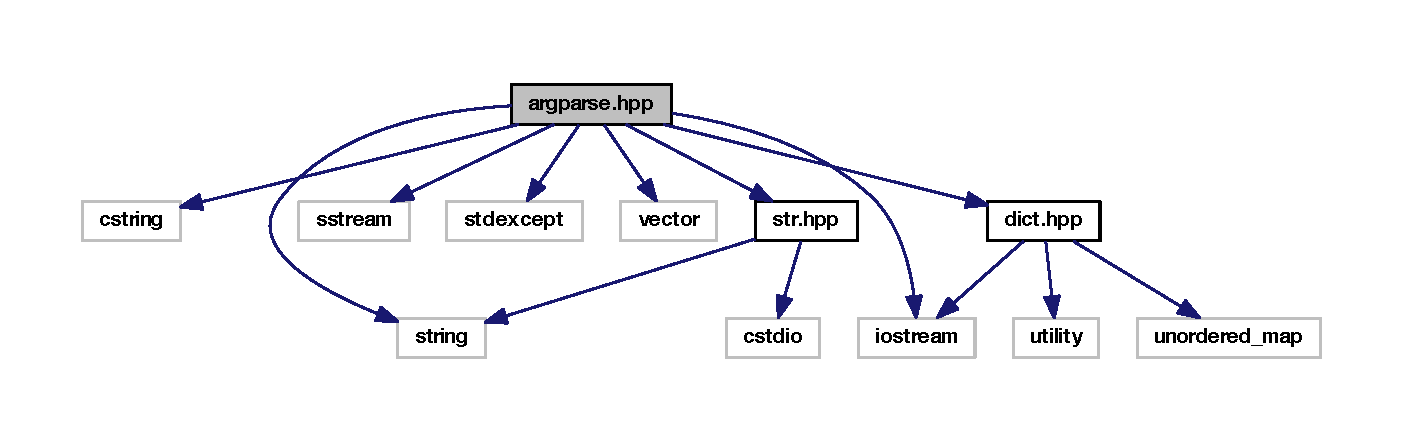
\includegraphics[width=350pt]{argparse_8hpp__incl}
\end{center}
\end{figure}
This graph shows which files directly or indirectly include this file\-:\nopagebreak
\begin{figure}[H]
\begin{center}
\leavevmode
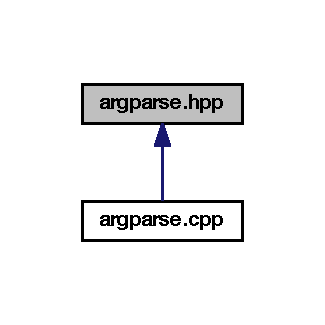
\includegraphics[width=156pt]{argparse_8hpp__dep__incl}
\end{center}
\end{figure}
\subsection*{Classes}
\begin{DoxyCompactItemize}
\item 
struct \hyperlink{structargparse_1_1_arg_holder}{argparse\-::\-Arg\-Holder}
\begin{DoxyCompactList}\small\item\em Holds the result of parsing arguments. \end{DoxyCompactList}\end{DoxyCompactItemize}
\subsection*{Namespaces}
\begin{DoxyCompactItemize}
\item 
namespace \hyperlink{namespaceargparse}{argparse}
\begin{DoxyCompactList}\small\item\em Command-\/line argument parser with a focus on brevity. \end{DoxyCompactList}\end{DoxyCompactItemize}
\subsection*{Functions}
\begin{DoxyCompactItemize}
\item 
string \hyperlink{namespaceargparse_a0ee3e8ca883816181b45c15a9ad0b6ed}{argparse\-::make\-Usage\-String} (const string \&prog\-Name, const string \&desc, const string \&pos\-Args=string(), const dict\-::\-Dict$<$ string, string $>$ \&opt\-To\-Help=dict\-::\-Dict$<$ string, string $>$(), unsigned cols=80, unsigned help\-Cols=60)
\begin{DoxyCompactList}\small\item\em Create a usage string. \end{DoxyCompactList}\item 
{\footnotesize template$<$class Func\-Type $>$ }\\Arg\-Holder \hyperlink{namespaceargparse_a4b1b6c03b45175acd13d1620f328e4aa}{argparse\-::parse} (int argc, const char $\ast$argv\mbox{[}$\,$\mbox{]}, const dict\-::\-Dict$<$ string, Func\-Type $>$ \&opt\-To\-Chker, char opt\-Char='-\/', bool gen\-Help\-Chker=true)
\begin{DoxyCompactList}\small\item\em Return an \hyperlink{structargparse_1_1_arg_holder}{Arg\-Holder} object holding the parsed arguments. \end{DoxyCompactList}\item 
\hyperlink{structargparse_1_1_arg_holder}{Arg\-Holder} \hyperlink{namespaceargparse_a6cfba06102a610840779069dfda1b98d}{argparse\-::parse} (int argc, const char $\ast$argv\mbox{[}$\,$\mbox{]}, const char opt\-Char='-\/', bool gen\-Help\-Chker=true)
\begin{DoxyCompactList}\small\item\em For programs that take no options. \end{DoxyCompactList}\end{DoxyCompactItemize}

\hypertarget{autodiff_8cpp}{\section{autodiff.\-cpp File Reference}
\label{autodiff_8cpp}\index{autodiff.\-cpp@{autodiff.\-cpp}}
}
{\ttfamily \#include $<$cmath$>$}\\*
{\ttfamily \#include $<$iostream$>$}\\*
{\ttfamily \#include \char`\"{}autodiff.\-hpp\char`\"{}}\\*
Include dependency graph for autodiff.\-cpp\-:\nopagebreak
\begin{figure}[H]
\begin{center}
\leavevmode
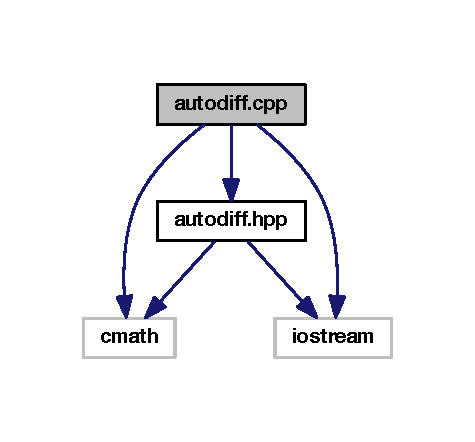
\includegraphics[width=228pt]{autodiff_8cpp__incl}
\end{center}
\end{figure}
\subsection*{Functions}
\begin{DoxyCompactItemize}
\item 
\hyperlink{structautodiff_1_1_dual_num}{Dual\-Num} \hyperlink{autodiff_8cpp_ae633308d2e5c4d2d185d53392e5b5b0a}{operator+} (const \hyperlink{structautodiff_1_1_dual_num}{Dual\-Num} \&a, const \hyperlink{structautodiff_1_1_dual_num}{Dual\-Num} \&b)
\item 
\hyperlink{structautodiff_1_1_dual_num}{Dual\-Num} \hyperlink{autodiff_8cpp_a787adac37341401ca38bde2c1825bf81}{operator-\/} (const \hyperlink{structautodiff_1_1_dual_num}{Dual\-Num} \&a, const \hyperlink{structautodiff_1_1_dual_num}{Dual\-Num} \&b)
\item 
\hyperlink{structautodiff_1_1_dual_num}{Dual\-Num} \hyperlink{autodiff_8cpp_a60637211a905130baeea07ba82cae9be}{operator-\/} (const \hyperlink{structautodiff_1_1_dual_num}{Dual\-Num} \&a)
\item 
\hyperlink{structautodiff_1_1_dual_num}{Dual\-Num} \hyperlink{autodiff_8cpp_a61d7fbca36cfb9a09a1726a2bfb82145}{operator$\ast$} (const \hyperlink{structautodiff_1_1_dual_num}{Dual\-Num} \&a, const \hyperlink{structautodiff_1_1_dual_num}{Dual\-Num} \&b)
\item 
\hyperlink{structautodiff_1_1_dual_num}{Dual\-Num} \hyperlink{autodiff_8cpp_a9726b843fee19d087ae7076cfe01ce12}{operator/} (const \hyperlink{structautodiff_1_1_dual_num}{Dual\-Num} \&a, const \hyperlink{structautodiff_1_1_dual_num}{Dual\-Num} \&b)
\item 
ostream \& \hyperlink{autodiff_8cpp_ab6b5f25da3be3e795c39283305527bb3}{operator$<$$<$} (ostream \&out, const \hyperlink{structautodiff_1_1_dual_num}{Dual\-Num} \&a)
\end{DoxyCompactItemize}


\subsection{Function Documentation}
\hypertarget{autodiff_8cpp_a61d7fbca36cfb9a09a1726a2bfb82145}{\index{autodiff.\-cpp@{autodiff.\-cpp}!operator$\ast$@{operator$\ast$}}
\index{operator$\ast$@{operator$\ast$}!autodiff.cpp@{autodiff.\-cpp}}
\subsubsection[{operator$\ast$}]{\setlength{\rightskip}{0pt plus 5cm}{\bf Dual\-Num} operator$\ast$ (
\begin{DoxyParamCaption}
\item[{const {\bf Dual\-Num} \&}]{a, }
\item[{const {\bf Dual\-Num} \&}]{b}
\end{DoxyParamCaption}
)}}\label{autodiff_8cpp_a61d7fbca36cfb9a09a1726a2bfb82145}
\hypertarget{autodiff_8cpp_ae633308d2e5c4d2d185d53392e5b5b0a}{\index{autodiff.\-cpp@{autodiff.\-cpp}!operator+@{operator+}}
\index{operator+@{operator+}!autodiff.cpp@{autodiff.\-cpp}}
\subsubsection[{operator+}]{\setlength{\rightskip}{0pt plus 5cm}{\bf Dual\-Num} operator+ (
\begin{DoxyParamCaption}
\item[{const {\bf Dual\-Num} \&}]{a, }
\item[{const {\bf Dual\-Num} \&}]{b}
\end{DoxyParamCaption}
)}}\label{autodiff_8cpp_ae633308d2e5c4d2d185d53392e5b5b0a}
\hypertarget{autodiff_8cpp_a787adac37341401ca38bde2c1825bf81}{\index{autodiff.\-cpp@{autodiff.\-cpp}!operator-\/@{operator-\/}}
\index{operator-\/@{operator-\/}!autodiff.cpp@{autodiff.\-cpp}}
\subsubsection[{operator-\/}]{\setlength{\rightskip}{0pt plus 5cm}{\bf Dual\-Num} operator-\/ (
\begin{DoxyParamCaption}
\item[{const {\bf Dual\-Num} \&}]{a, }
\item[{const {\bf Dual\-Num} \&}]{b}
\end{DoxyParamCaption}
)}}\label{autodiff_8cpp_a787adac37341401ca38bde2c1825bf81}
\hypertarget{autodiff_8cpp_a60637211a905130baeea07ba82cae9be}{\index{autodiff.\-cpp@{autodiff.\-cpp}!operator-\/@{operator-\/}}
\index{operator-\/@{operator-\/}!autodiff.cpp@{autodiff.\-cpp}}
\subsubsection[{operator-\/}]{\setlength{\rightskip}{0pt plus 5cm}{\bf Dual\-Num} operator-\/ (
\begin{DoxyParamCaption}
\item[{const {\bf Dual\-Num} \&}]{a}
\end{DoxyParamCaption}
)}}\label{autodiff_8cpp_a60637211a905130baeea07ba82cae9be}
\hypertarget{autodiff_8cpp_a9726b843fee19d087ae7076cfe01ce12}{\index{autodiff.\-cpp@{autodiff.\-cpp}!operator/@{operator/}}
\index{operator/@{operator/}!autodiff.cpp@{autodiff.\-cpp}}
\subsubsection[{operator/}]{\setlength{\rightskip}{0pt plus 5cm}{\bf Dual\-Num} operator/ (
\begin{DoxyParamCaption}
\item[{const {\bf Dual\-Num} \&}]{a, }
\item[{const {\bf Dual\-Num} \&}]{b}
\end{DoxyParamCaption}
)}}\label{autodiff_8cpp_a9726b843fee19d087ae7076cfe01ce12}
\hypertarget{autodiff_8cpp_ab6b5f25da3be3e795c39283305527bb3}{\index{autodiff.\-cpp@{autodiff.\-cpp}!operator$<$$<$@{operator$<$$<$}}
\index{operator$<$$<$@{operator$<$$<$}!autodiff.cpp@{autodiff.\-cpp}}
\subsubsection[{operator$<$$<$}]{\setlength{\rightskip}{0pt plus 5cm}ostream\& operator$<$$<$ (
\begin{DoxyParamCaption}
\item[{ostream \&}]{out, }
\item[{const {\bf Dual\-Num} \&}]{a}
\end{DoxyParamCaption}
)}}\label{autodiff_8cpp_ab6b5f25da3be3e795c39283305527bb3}

\hypertarget{autodiff_8hpp}{\section{autodiff.\-hpp File Reference}
\label{autodiff_8hpp}\index{autodiff.\-hpp@{autodiff.\-hpp}}
}
{\ttfamily \#include $<$cmath$>$}\\*
{\ttfamily \#include $<$iostream$>$}\\*
\subsection*{Classes}
\begin{DoxyCompactItemize}
\item 
struct \hyperlink{structautodiff_1_1_dual_num}{autodiff\-::\-Dual\-Num}
\begin{DoxyCompactList}\small\item\em Represents the \char`\"{}real\char`\"{} part of a number in member {\ttfamily r} and the derivative in {\ttfamily d}. \end{DoxyCompactList}\end{DoxyCompactItemize}
\subsection*{Namespaces}
\begin{DoxyCompactItemize}
\item 
namespace \hyperlink{namespaceautodiff}{autodiff}
\begin{DoxyCompactList}\small\item\em Implements automatic differentiation. \end{DoxyCompactList}\end{DoxyCompactItemize}
\subsection*{Functions}
\begin{DoxyCompactItemize}
\item 
\hyperlink{structautodiff_1_1_dual_num}{Dual\-Num} \hyperlink{namespaceautodiff_a19b889e35f523cc6ca0f377dc8bed262}{autodiff\-::d\-Pow} (const \hyperlink{structautodiff_1_1_dual_num}{Dual\-Num} \&a, const \hyperlink{structautodiff_1_1_dual_num}{Dual\-Num} \&b)
\item 
\hyperlink{structautodiff_1_1_dual_num}{Dual\-Num} \hyperlink{namespaceautodiff_a0f6df25515f7f05f838a9fd96f53fd37}{autodiff\-::d\-Sin} (const \hyperlink{structautodiff_1_1_dual_num}{Dual\-Num} \&a)
\item 
\hyperlink{structautodiff_1_1_dual_num}{Dual\-Num} \hyperlink{namespaceautodiff_a49d66a6f54fffb4250795cc589158a14}{autodiff\-::d\-Cos} (const \hyperlink{structautodiff_1_1_dual_num}{Dual\-Num} \&a)
\item 
\hyperlink{structautodiff_1_1_dual_num}{Dual\-Num} \hyperlink{namespaceautodiff_a4bdb0754d9ad8a5c4aba2d7ea9f040db}{autodiff\-::d\-Tan} (const \hyperlink{structautodiff_1_1_dual_num}{Dual\-Num} \&a)
\item 
\hyperlink{structautodiff_1_1_dual_num}{Dual\-Num} \hyperlink{namespaceautodiff_af2706967e031d3472b823760b0c67dcb}{autodiff\-::d\-Exp} (const \hyperlink{structautodiff_1_1_dual_num}{Dual\-Num} \&a)
\item 
\hyperlink{structautodiff_1_1_dual_num}{Dual\-Num} \hyperlink{namespaceautodiff_a003e7455b4727bad71fdb9b6bc676e86}{autodiff\-::d\-Log} (const \hyperlink{structautodiff_1_1_dual_num}{Dual\-Num} \&a)
\item 
\hyperlink{structautodiff_1_1_dual_num}{Dual\-Num} \hyperlink{namespaceautodiff_a656dafc1fc9422d40ade97d24905f875}{autodiff\-::d\-Log10} (const \hyperlink{structautodiff_1_1_dual_num}{Dual\-Num} \&a)
\item 
\hyperlink{structautodiff_1_1_dual_num}{autodiff\-::\-Dual\-Num} \hyperlink{autodiff_8hpp_afcaa49648f532c1593415c845c2fdba6}{operator+} (const \hyperlink{structautodiff_1_1_dual_num}{autodiff\-::\-Dual\-Num} \&a, const \hyperlink{structautodiff_1_1_dual_num}{autodiff\-::\-Dual\-Num} \&b)
\item 
\hyperlink{structautodiff_1_1_dual_num}{autodiff\-::\-Dual\-Num} \hyperlink{autodiff_8hpp_a74872447d0a3ced20978ab51ee1f657d}{operator-\/} (const \hyperlink{structautodiff_1_1_dual_num}{autodiff\-::\-Dual\-Num} \&a, const \hyperlink{structautodiff_1_1_dual_num}{autodiff\-::\-Dual\-Num} \&b)
\item 
\hyperlink{structautodiff_1_1_dual_num}{autodiff\-::\-Dual\-Num} \hyperlink{autodiff_8hpp_a5b2488b390f5cf4f33ba2d057209eace}{operator-\/} (const \hyperlink{structautodiff_1_1_dual_num}{autodiff\-::\-Dual\-Num} \&a)
\item 
\hyperlink{structautodiff_1_1_dual_num}{autodiff\-::\-Dual\-Num} \hyperlink{autodiff_8hpp_a87030a560abe7446ab81995b3724cc51}{operator$\ast$} (const \hyperlink{structautodiff_1_1_dual_num}{autodiff\-::\-Dual\-Num} \&a, const \hyperlink{structautodiff_1_1_dual_num}{autodiff\-::\-Dual\-Num} \&b)
\item 
\hyperlink{structautodiff_1_1_dual_num}{autodiff\-::\-Dual\-Num} \hyperlink{autodiff_8hpp_a0fa02b284f6ac59a838b8458d2dc381b}{operator/} (const \hyperlink{structautodiff_1_1_dual_num}{autodiff\-::\-Dual\-Num} \&a, const \hyperlink{structautodiff_1_1_dual_num}{autodiff\-::\-Dual\-Num} \&b)
\item 
ostream \& \hyperlink{autodiff_8hpp_aba8d3eb9946f938d7ea0f6980732bfb5}{operator$<$$<$} (ostream \&out, const \hyperlink{structautodiff_1_1_dual_num}{autodiff\-::\-Dual\-Num} \&a)
\end{DoxyCompactItemize}
\subsection*{Variables}
\begin{DoxyCompactItemize}
\item 
const double \hyperlink{namespaceautodiff_ac438d71cd4847e9f19efe6a4f1cfd5d7}{autodiff\-::\-I\-N\-V\-\_\-\-L\-O\-G\-\_\-10} = 1 / log(10)
\end{DoxyCompactItemize}


\subsection{Function Documentation}
\hypertarget{autodiff_8hpp_a87030a560abe7446ab81995b3724cc51}{\index{autodiff.\-hpp@{autodiff.\-hpp}!operator$\ast$@{operator$\ast$}}
\index{operator$\ast$@{operator$\ast$}!autodiff.hpp@{autodiff.\-hpp}}
\subsubsection[{operator$\ast$}]{\setlength{\rightskip}{0pt plus 5cm}{\bf autodiff\-::\-Dual\-Num} operator$\ast$ (
\begin{DoxyParamCaption}
\item[{const {\bf autodiff\-::\-Dual\-Num} \&}]{a, }
\item[{const {\bf autodiff\-::\-Dual\-Num} \&}]{b}
\end{DoxyParamCaption}
)}}\label{autodiff_8hpp_a87030a560abe7446ab81995b3724cc51}
\hypertarget{autodiff_8hpp_afcaa49648f532c1593415c845c2fdba6}{\index{autodiff.\-hpp@{autodiff.\-hpp}!operator+@{operator+}}
\index{operator+@{operator+}!autodiff.hpp@{autodiff.\-hpp}}
\subsubsection[{operator+}]{\setlength{\rightskip}{0pt plus 5cm}{\bf autodiff\-::\-Dual\-Num} operator+ (
\begin{DoxyParamCaption}
\item[{const {\bf autodiff\-::\-Dual\-Num} \&}]{a, }
\item[{const {\bf autodiff\-::\-Dual\-Num} \&}]{b}
\end{DoxyParamCaption}
)}}\label{autodiff_8hpp_afcaa49648f532c1593415c845c2fdba6}
\hypertarget{autodiff_8hpp_a74872447d0a3ced20978ab51ee1f657d}{\index{autodiff.\-hpp@{autodiff.\-hpp}!operator-\/@{operator-\/}}
\index{operator-\/@{operator-\/}!autodiff.hpp@{autodiff.\-hpp}}
\subsubsection[{operator-\/}]{\setlength{\rightskip}{0pt plus 5cm}{\bf autodiff\-::\-Dual\-Num} operator-\/ (
\begin{DoxyParamCaption}
\item[{const {\bf autodiff\-::\-Dual\-Num} \&}]{a, }
\item[{const {\bf autodiff\-::\-Dual\-Num} \&}]{b}
\end{DoxyParamCaption}
)}}\label{autodiff_8hpp_a74872447d0a3ced20978ab51ee1f657d}
\hypertarget{autodiff_8hpp_a5b2488b390f5cf4f33ba2d057209eace}{\index{autodiff.\-hpp@{autodiff.\-hpp}!operator-\/@{operator-\/}}
\index{operator-\/@{operator-\/}!autodiff.hpp@{autodiff.\-hpp}}
\subsubsection[{operator-\/}]{\setlength{\rightskip}{0pt plus 5cm}{\bf autodiff\-::\-Dual\-Num} operator-\/ (
\begin{DoxyParamCaption}
\item[{const {\bf autodiff\-::\-Dual\-Num} \&}]{a}
\end{DoxyParamCaption}
)}}\label{autodiff_8hpp_a5b2488b390f5cf4f33ba2d057209eace}
\hypertarget{autodiff_8hpp_a0fa02b284f6ac59a838b8458d2dc381b}{\index{autodiff.\-hpp@{autodiff.\-hpp}!operator/@{operator/}}
\index{operator/@{operator/}!autodiff.hpp@{autodiff.\-hpp}}
\subsubsection[{operator/}]{\setlength{\rightskip}{0pt plus 5cm}{\bf autodiff\-::\-Dual\-Num} operator/ (
\begin{DoxyParamCaption}
\item[{const {\bf autodiff\-::\-Dual\-Num} \&}]{a, }
\item[{const {\bf autodiff\-::\-Dual\-Num} \&}]{b}
\end{DoxyParamCaption}
)}}\label{autodiff_8hpp_a0fa02b284f6ac59a838b8458d2dc381b}
\hypertarget{autodiff_8hpp_aba8d3eb9946f938d7ea0f6980732bfb5}{\index{autodiff.\-hpp@{autodiff.\-hpp}!operator$<$$<$@{operator$<$$<$}}
\index{operator$<$$<$@{operator$<$$<$}!autodiff.hpp@{autodiff.\-hpp}}
\subsubsection[{operator$<$$<$}]{\setlength{\rightskip}{0pt plus 5cm}ostream\& operator$<$$<$ (
\begin{DoxyParamCaption}
\item[{ostream \&}]{out, }
\item[{const {\bf autodiff\-::\-Dual\-Num} \&}]{a}
\end{DoxyParamCaption}
)}}\label{autodiff_8hpp_aba8d3eb9946f938d7ea0f6980732bfb5}

\hypertarget{cvutils_8cpp}{\section{cvutils.\-cpp File Reference}
\label{cvutils_8cpp}\index{cvutils.\-cpp@{cvutils.\-cpp}}
}
{\ttfamily \#include $<$cstdint$>$}\\*
{\ttfamily \#include $<$algorithm$>$}\\*
{\ttfamily \#include $<$iostream$>$}\\*
{\ttfamily \#include $<$opencv2/opencv.\-hpp$>$}\\*
{\ttfamily \#include \char`\"{}cvutils.\-hpp\char`\"{}}\\*
{\ttfamily \#include \char`\"{}kmath.\-hpp\char`\"{}}\\*
Include dependency graph for cvutils.\-cpp\-:
\nopagebreak
\begin{figure}[H]
\begin{center}
\leavevmode
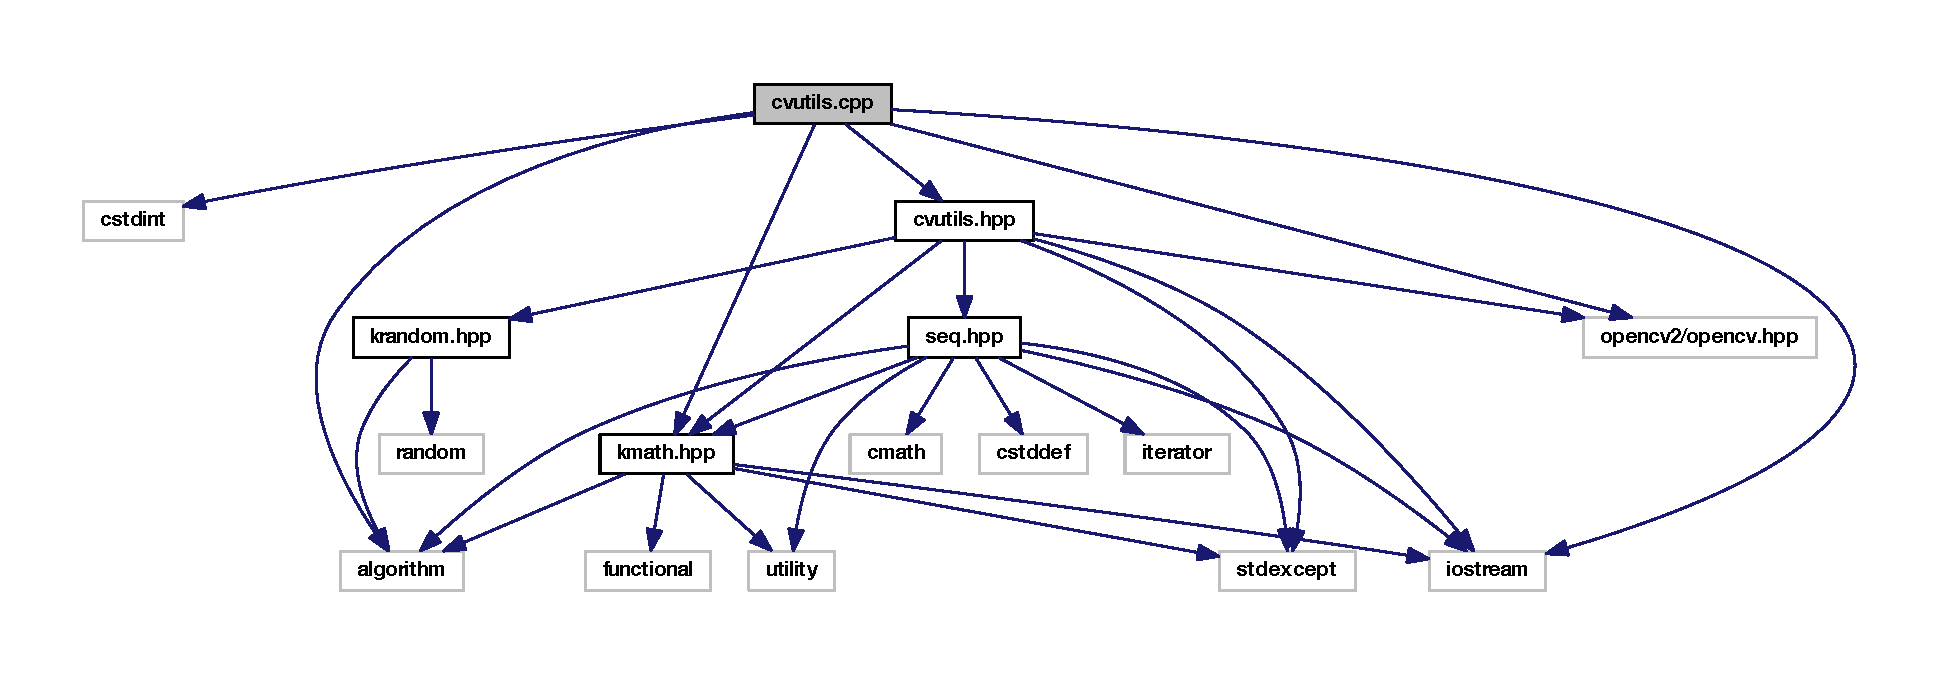
\includegraphics[width=350pt]{cvutils_8cpp__incl}
\end{center}
\end{figure}
\subsection*{Functions}
\begin{DoxyCompactItemize}
\item 
ostream \& \hyperlink{cvutils_8cpp_a8e51a09bac9db8fc1086987161a5cde6}{operator$<$$<$} (ostream \&out, const Rect r)
\item 
ostream \& \hyperlink{cvutils_8cpp_a40e1aedcd73028caaf91a9799864d28b}{operator$<$$<$} (ostream \&out, const Size s)
\item 
ostream \& \hyperlink{cvutils_8cpp_ad24b7492cab7eddd53c2c12e61b21f13}{operator$<$$<$} (ostream \&out, const Size2f s)
\item 
ostream \& \hyperlink{cvutils_8cpp_aeaadaf0340a8cbab0ebe95c6d838e3d5}{operator$<$$<$} (ostream \&out, const Scalar s)
\item 
ostream \& \hyperlink{cvutils_8cpp_a19e2583b33817fa0157b7ba5d0ef42cb}{operator$<$$<$} (ostream \&out, const uchar c)
\item 
Size2f \hyperlink{cvutils_8cpp_ae180673a678e0c21b86f8c289c096c9a}{operator$\ast$} (const Size2f \&s, float a)
\item 
Size2f \hyperlink{cvutils_8cpp_aa0e8d1466faa50fc2e5d39500a83f3ad}{operator$\ast$} (float a, const Size2f \&s)
\item 
Size2f \hyperlink{cvutils_8cpp_aa6299a78aae948a9d8a8f5dfbc8c1305}{operator/} (const Size2f \&s, float a)
\item 
bool \hyperlink{cvutils_8cpp_a1d6da8c1cf5d528e8eeaefcc12e7ab85}{operator==} (const Size2f \&a, const Size2f \&b)
\item 
bool \hyperlink{cvutils_8cpp_acff1ba895a3cb7b31c791335098eca94}{operator!=} (const Size2f \&a, const Size2f \&b)
\end{DoxyCompactItemize}


\subsection{Function Documentation}
\hypertarget{cvutils_8cpp_a8e51a09bac9db8fc1086987161a5cde6}{\index{cvutils.\-cpp@{cvutils.\-cpp}!operator$<$$<$@{operator$<$$<$}}
\index{operator$<$$<$@{operator$<$$<$}!cvutils.cpp@{cvutils.\-cpp}}
\subsubsection[{operator$<$$<$}]{\setlength{\rightskip}{0pt plus 5cm}ostream\& operator$<$$<$ (
\begin{DoxyParamCaption}
\item[{ostream \&}]{out, }
\item[{const Rect}]{r}
\end{DoxyParamCaption}
)}}\label{cvutils_8cpp_a8e51a09bac9db8fc1086987161a5cde6}
\hypertarget{cvutils_8cpp_a40e1aedcd73028caaf91a9799864d28b}{\index{cvutils.\-cpp@{cvutils.\-cpp}!operator$<$$<$@{operator$<$$<$}}
\index{operator$<$$<$@{operator$<$$<$}!cvutils.cpp@{cvutils.\-cpp}}
\subsubsection[{operator$<$$<$}]{\setlength{\rightskip}{0pt plus 5cm}ostream\& operator$<$$<$ (
\begin{DoxyParamCaption}
\item[{ostream \&}]{out, }
\item[{const Size}]{s}
\end{DoxyParamCaption}
)}}\label{cvutils_8cpp_a40e1aedcd73028caaf91a9799864d28b}
\hypertarget{cvutils_8cpp_ad24b7492cab7eddd53c2c12e61b21f13}{\index{cvutils.\-cpp@{cvutils.\-cpp}!operator$<$$<$@{operator$<$$<$}}
\index{operator$<$$<$@{operator$<$$<$}!cvutils.cpp@{cvutils.\-cpp}}
\subsubsection[{operator$<$$<$}]{\setlength{\rightskip}{0pt plus 5cm}ostream\& operator$<$$<$ (
\begin{DoxyParamCaption}
\item[{ostream \&}]{out, }
\item[{const Size2f}]{s}
\end{DoxyParamCaption}
)}}\label{cvutils_8cpp_ad24b7492cab7eddd53c2c12e61b21f13}
\hypertarget{cvutils_8cpp_aeaadaf0340a8cbab0ebe95c6d838e3d5}{\index{cvutils.\-cpp@{cvutils.\-cpp}!operator$<$$<$@{operator$<$$<$}}
\index{operator$<$$<$@{operator$<$$<$}!cvutils.cpp@{cvutils.\-cpp}}
\subsubsection[{operator$<$$<$}]{\setlength{\rightskip}{0pt plus 5cm}ostream\& operator$<$$<$ (
\begin{DoxyParamCaption}
\item[{ostream \&}]{out, }
\item[{const Scalar}]{s}
\end{DoxyParamCaption}
)}}\label{cvutils_8cpp_aeaadaf0340a8cbab0ebe95c6d838e3d5}
\hypertarget{cvutils_8cpp_a19e2583b33817fa0157b7ba5d0ef42cb}{\index{cvutils.\-cpp@{cvutils.\-cpp}!operator$<$$<$@{operator$<$$<$}}
\index{operator$<$$<$@{operator$<$$<$}!cvutils.cpp@{cvutils.\-cpp}}
\subsubsection[{operator$<$$<$}]{\setlength{\rightskip}{0pt plus 5cm}ostream\& operator$<$$<$ (
\begin{DoxyParamCaption}
\item[{ostream \&}]{out, }
\item[{const uchar}]{c}
\end{DoxyParamCaption}
)}}\label{cvutils_8cpp_a19e2583b33817fa0157b7ba5d0ef42cb}
\hypertarget{cvutils_8cpp_ae180673a678e0c21b86f8c289c096c9a}{\index{cvutils.\-cpp@{cvutils.\-cpp}!operator$\ast$@{operator$\ast$}}
\index{operator$\ast$@{operator$\ast$}!cvutils.cpp@{cvutils.\-cpp}}
\subsubsection[{operator$\ast$}]{\setlength{\rightskip}{0pt plus 5cm}Size2f operator$\ast$ (
\begin{DoxyParamCaption}
\item[{const Size2f \&}]{s, }
\item[{float}]{a}
\end{DoxyParamCaption}
)}}\label{cvutils_8cpp_ae180673a678e0c21b86f8c289c096c9a}
\hypertarget{cvutils_8cpp_aa0e8d1466faa50fc2e5d39500a83f3ad}{\index{cvutils.\-cpp@{cvutils.\-cpp}!operator$\ast$@{operator$\ast$}}
\index{operator$\ast$@{operator$\ast$}!cvutils.cpp@{cvutils.\-cpp}}
\subsubsection[{operator$\ast$}]{\setlength{\rightskip}{0pt plus 5cm}Size2f operator$\ast$ (
\begin{DoxyParamCaption}
\item[{float}]{a, }
\item[{const Size2f \&}]{s}
\end{DoxyParamCaption}
)}}\label{cvutils_8cpp_aa0e8d1466faa50fc2e5d39500a83f3ad}
\hypertarget{cvutils_8cpp_aa6299a78aae948a9d8a8f5dfbc8c1305}{\index{cvutils.\-cpp@{cvutils.\-cpp}!operator/@{operator/}}
\index{operator/@{operator/}!cvutils.cpp@{cvutils.\-cpp}}
\subsubsection[{operator/}]{\setlength{\rightskip}{0pt plus 5cm}Size2f operator/ (
\begin{DoxyParamCaption}
\item[{const Size2f \&}]{s, }
\item[{float}]{a}
\end{DoxyParamCaption}
)}}\label{cvutils_8cpp_aa6299a78aae948a9d8a8f5dfbc8c1305}
\hypertarget{cvutils_8cpp_a1d6da8c1cf5d528e8eeaefcc12e7ab85}{\index{cvutils.\-cpp@{cvutils.\-cpp}!operator==@{operator==}}
\index{operator==@{operator==}!cvutils.cpp@{cvutils.\-cpp}}
\subsubsection[{operator==}]{\setlength{\rightskip}{0pt plus 5cm}bool operator== (
\begin{DoxyParamCaption}
\item[{const Size2f \&}]{a, }
\item[{const Size2f \&}]{b}
\end{DoxyParamCaption}
)}}\label{cvutils_8cpp_a1d6da8c1cf5d528e8eeaefcc12e7ab85}
\hypertarget{cvutils_8cpp_acff1ba895a3cb7b31c791335098eca94}{\index{cvutils.\-cpp@{cvutils.\-cpp}!operator!=@{operator!=}}
\index{operator!=@{operator!=}!cvutils.cpp@{cvutils.\-cpp}}
\subsubsection[{operator!=}]{\setlength{\rightskip}{0pt plus 5cm}bool operator!= (
\begin{DoxyParamCaption}
\item[{const Size2f \&}]{a, }
\item[{const Size2f \&}]{b}
\end{DoxyParamCaption}
)}}\label{cvutils_8cpp_acff1ba895a3cb7b31c791335098eca94}

\hypertarget{cvutils_8hpp}{\section{cvutils.\-hpp File Reference}
\label{cvutils_8hpp}\index{cvutils.\-hpp@{cvutils.\-hpp}}
}
{\ttfamily \#include $<$iostream$>$}\\*
{\ttfamily \#include $<$opencv2/opencv.\-hpp$>$}\\*
\subsection*{Classes}
\begin{DoxyCompactItemize}
\item 
struct \hyperlink{structcvutils_1_1___data_depth___fixed}{cvutils\-::\-\_\-\-Data\-Depth\-\_\-\-Fixed$<$ T $>$}
\item 
struct \hyperlink{structcvutils_1_1___data_depth___fixed_3_01uchar_01_4}{cvutils\-::\-\_\-\-Data\-Depth\-\_\-\-Fixed$<$ uchar $>$}
\end{DoxyCompactItemize}
\subsection*{Namespaces}
\begin{DoxyCompactItemize}
\item 
namespace \hyperlink{namespacecvutils}{cvutils}
\begin{DoxyCompactList}\small\item\em Open\-C\-V utilities. \end{DoxyCompactList}\end{DoxyCompactItemize}
\subsection*{Functions}
\begin{DoxyCompactItemize}
\item 
void \hyperlink{namespacecvutils_aa292da4b50c7692374fdde56afdd6baf}{cvutils\-::wait\-For\-Keypress} ()
\item 
ostream \& \hyperlink{cvutils_8hpp_a0b14696e4e43f7a2a1e707fa208b4ea6}{operator$<$$<$} (ostream \&out, const cv\-::\-Rect r)
\item 
ostream \& \hyperlink{cvutils_8hpp_acac9a564a7e46f10e2e1603edac9e540}{operator$<$$<$} (ostream \&out, const cv\-::\-Size s)
\item 
ostream \& \hyperlink{cvutils_8hpp_a5b3e75872c29d47c8c8fe2226927b511}{operator$<$$<$} (ostream \&out, const cv\-::\-Size2f s)
\item 
ostream \& \hyperlink{cvutils_8hpp_a4ca6efe2216f3d895e6de2a5cec34fc1}{operator$<$$<$} (ostream \&out, const cv\-::\-Scalar s)
\item 
ostream \& \hyperlink{cvutils_8hpp_a19e2583b33817fa0157b7ba5d0ef42cb}{operator$<$$<$} (ostream \&out, const uchar c)
\item 
{\footnotesize template$<$typename T , int cn$>$ }\\ostream \& \hyperlink{cvutils_8hpp_a2a8d9a7b33a01731771e3ef6a6fbfa7f}{operator$<$$<$} (ostream \&out, const cv\-::\-Vec$<$ T, cn $>$ v)
\end{DoxyCompactItemize}


\subsection{Function Documentation}
\hypertarget{cvutils_8hpp_a0b14696e4e43f7a2a1e707fa208b4ea6}{\index{cvutils.\-hpp@{cvutils.\-hpp}!operator$<$$<$@{operator$<$$<$}}
\index{operator$<$$<$@{operator$<$$<$}!cvutils.hpp@{cvutils.\-hpp}}
\subsubsection[{operator$<$$<$}]{\setlength{\rightskip}{0pt plus 5cm}ostream\& operator$<$$<$ (
\begin{DoxyParamCaption}
\item[{ostream \&}]{out, }
\item[{const cv\-::\-Rect}]{r}
\end{DoxyParamCaption}
)}}\label{cvutils_8hpp_a0b14696e4e43f7a2a1e707fa208b4ea6}
\hypertarget{cvutils_8hpp_acac9a564a7e46f10e2e1603edac9e540}{\index{cvutils.\-hpp@{cvutils.\-hpp}!operator$<$$<$@{operator$<$$<$}}
\index{operator$<$$<$@{operator$<$$<$}!cvutils.hpp@{cvutils.\-hpp}}
\subsubsection[{operator$<$$<$}]{\setlength{\rightskip}{0pt plus 5cm}ostream\& operator$<$$<$ (
\begin{DoxyParamCaption}
\item[{ostream \&}]{out, }
\item[{const cv\-::\-Size}]{s}
\end{DoxyParamCaption}
)}}\label{cvutils_8hpp_acac9a564a7e46f10e2e1603edac9e540}
\hypertarget{cvutils_8hpp_a5b3e75872c29d47c8c8fe2226927b511}{\index{cvutils.\-hpp@{cvutils.\-hpp}!operator$<$$<$@{operator$<$$<$}}
\index{operator$<$$<$@{operator$<$$<$}!cvutils.hpp@{cvutils.\-hpp}}
\subsubsection[{operator$<$$<$}]{\setlength{\rightskip}{0pt plus 5cm}ostream\& operator$<$$<$ (
\begin{DoxyParamCaption}
\item[{ostream \&}]{out, }
\item[{const cv\-::\-Size2f}]{s}
\end{DoxyParamCaption}
)}}\label{cvutils_8hpp_a5b3e75872c29d47c8c8fe2226927b511}
\hypertarget{cvutils_8hpp_a4ca6efe2216f3d895e6de2a5cec34fc1}{\index{cvutils.\-hpp@{cvutils.\-hpp}!operator$<$$<$@{operator$<$$<$}}
\index{operator$<$$<$@{operator$<$$<$}!cvutils.hpp@{cvutils.\-hpp}}
\subsubsection[{operator$<$$<$}]{\setlength{\rightskip}{0pt plus 5cm}ostream\& operator$<$$<$ (
\begin{DoxyParamCaption}
\item[{ostream \&}]{out, }
\item[{const cv\-::\-Scalar}]{s}
\end{DoxyParamCaption}
)}}\label{cvutils_8hpp_a4ca6efe2216f3d895e6de2a5cec34fc1}
\hypertarget{cvutils_8hpp_a19e2583b33817fa0157b7ba5d0ef42cb}{\index{cvutils.\-hpp@{cvutils.\-hpp}!operator$<$$<$@{operator$<$$<$}}
\index{operator$<$$<$@{operator$<$$<$}!cvutils.hpp@{cvutils.\-hpp}}
\subsubsection[{operator$<$$<$}]{\setlength{\rightskip}{0pt plus 5cm}ostream\& operator$<$$<$ (
\begin{DoxyParamCaption}
\item[{ostream \&}]{out, }
\item[{const uchar}]{c}
\end{DoxyParamCaption}
)}}\label{cvutils_8hpp_a19e2583b33817fa0157b7ba5d0ef42cb}
\hypertarget{cvutils_8hpp_a2a8d9a7b33a01731771e3ef6a6fbfa7f}{\index{cvutils.\-hpp@{cvutils.\-hpp}!operator$<$$<$@{operator$<$$<$}}
\index{operator$<$$<$@{operator$<$$<$}!cvutils.hpp@{cvutils.\-hpp}}
\subsubsection[{operator$<$$<$}]{\setlength{\rightskip}{0pt plus 5cm}template$<$typename T , int cn$>$ ostream\& operator$<$$<$ (
\begin{DoxyParamCaption}
\item[{ostream \&}]{out, }
\item[{const cv\-::\-Vec$<$ T, cn $>$}]{v}
\end{DoxyParamCaption}
)}}\label{cvutils_8hpp_a2a8d9a7b33a01731771e3ef6a6fbfa7f}

\hypertarget{dict_8hpp}{\section{dict.\-hpp File Reference}
\label{dict_8hpp}\index{dict.\-hpp@{dict.\-hpp}}
}
{\ttfamily \#include $<$unordered\-\_\-map$>$}\\*
{\ttfamily \#include $<$utility$>$}\\*
\subsection*{Namespaces}
\begin{DoxyCompactItemize}
\item 
namespace \hyperlink{namespacedict}{dict}
\begin{DoxyCompactList}\small\item\em Utilities for working with {\ttfamily Dict}s ({\ttfamily unordered\-\_\-map}s). \end{DoxyCompactList}\end{DoxyCompactItemize}
\subsection*{Functions}
\begin{DoxyCompactItemize}
\item 
{\footnotesize template$<$typename Key\-Type , typename Val\-Type $>$ }\\void \hyperlink{dict_8hpp_aad450cc243fecdc56252ec17b2c7f242}{\-\_\-make\-Dict\-I\-P} (Dict$<$ Key\-Type, Val\-Type $>$ \&d, Key\-Type key, Val\-Type val)
\item 
{\footnotesize template$<$typename Key\-Type , typename Val\-Type , typename... Args$>$ }\\void \hyperlink{dict_8hpp_a63c4edeb75c1a98c92321da3c0feb818}{\-\_\-make\-Dict\-I\-P} (Dict$<$ Key\-Type, Val\-Type $>$ \&d, Key\-Type key, Val\-Type val, Args...\-args)
\item 
{\footnotesize template$<$typename Key\-Type , typename Val\-Type , typename... Args$>$ }\\Dict$<$ Key\-Type, Val\-Type $>$ \hyperlink{dict_8hpp_acf532dcb9ac916d2ac99b609a3a2422d}{make\-Dict} (Key\-Type key, Val\-Type val, Args...\-args)
\item 
{\footnotesize template$<$typename Key\-Type , typename Val\-Type $>$ }\\Dict$<$ Key\-Type, Val\-Type $>$ \hyperlink{dict_8hpp_a952263572be8fc115fb88a93631e6fc3}{make\-Dict} ()
\item 
{\footnotesize template$<$typename Key\-T , typename Val\-T $>$ }\\ostream \& \hyperlink{dict_8hpp_a3c4515d6a24ee85ca1ff76eff687c06b}{operator$<$$<$} (ostream \&out, const Dict$<$ Key\-T, Val\-T $>$ \&seq)
\item 
{\footnotesize template$<$typename Iter\-T , typename Elem\-T $>$ }\\Dict$<$ Elem\-T, unsigned $>$ \& \hyperlink{namespacedict_a25d4adabc11b7754dad27d591de51df6}{dict\-::count\-Elems} (const Iter\-T \&start, const Iter\-T \&end, Dict$<$ Elem\-T, unsigned $>$ \&out)
\end{DoxyCompactItemize}


\subsection{Function Documentation}
\hypertarget{dict_8hpp_aad450cc243fecdc56252ec17b2c7f242}{\index{dict.\-hpp@{dict.\-hpp}!\-\_\-make\-Dict\-I\-P@{\-\_\-make\-Dict\-I\-P}}
\index{\-\_\-make\-Dict\-I\-P@{\-\_\-make\-Dict\-I\-P}!dict.hpp@{dict.\-hpp}}
\subsubsection[{\-\_\-make\-Dict\-I\-P}]{\setlength{\rightskip}{0pt plus 5cm}template$<$typename Key\-Type , typename Val\-Type $>$ void {\bf \-\_\-make\-Dict\-I\-P} (
\begin{DoxyParamCaption}
\item[{Dict$<$ Key\-Type, Val\-Type $>$ \&}]{d, }
\item[{Key\-Type}]{key, }
\item[{Val\-Type}]{val}
\end{DoxyParamCaption}
)}}\label{dict_8hpp_aad450cc243fecdc56252ec17b2c7f242}
\hypertarget{dict_8hpp_a63c4edeb75c1a98c92321da3c0feb818}{\index{dict.\-hpp@{dict.\-hpp}!\-\_\-make\-Dict\-I\-P@{\-\_\-make\-Dict\-I\-P}}
\index{\-\_\-make\-Dict\-I\-P@{\-\_\-make\-Dict\-I\-P}!dict.hpp@{dict.\-hpp}}
\subsubsection[{\-\_\-make\-Dict\-I\-P}]{\setlength{\rightskip}{0pt plus 5cm}template$<$typename Key\-Type , typename Val\-Type , typename... Args$>$ void {\bf \-\_\-make\-Dict\-I\-P} (
\begin{DoxyParamCaption}
\item[{Dict$<$ Key\-Type, Val\-Type $>$ \&}]{d, }
\item[{Key\-Type}]{key, }
\item[{Val\-Type}]{val, }
\item[{Args...}]{args}
\end{DoxyParamCaption}
)}}\label{dict_8hpp_a63c4edeb75c1a98c92321da3c0feb818}
\hypertarget{dict_8hpp_acf532dcb9ac916d2ac99b609a3a2422d}{\index{dict.\-hpp@{dict.\-hpp}!make\-Dict@{make\-Dict}}
\index{make\-Dict@{make\-Dict}!dict.hpp@{dict.\-hpp}}
\subsubsection[{make\-Dict}]{\setlength{\rightskip}{0pt plus 5cm}template$<$typename Key\-Type , typename Val\-Type , typename... Args$>$ Dict$<$Key\-Type, Val\-Type$>$ {\bf make\-Dict} (
\begin{DoxyParamCaption}
\item[{Key\-Type}]{key, }
\item[{Val\-Type}]{val, }
\item[{Args...}]{args}
\end{DoxyParamCaption}
)}}\label{dict_8hpp_acf532dcb9ac916d2ac99b609a3a2422d}
\hypertarget{dict_8hpp_a952263572be8fc115fb88a93631e6fc3}{\index{dict.\-hpp@{dict.\-hpp}!make\-Dict@{make\-Dict}}
\index{make\-Dict@{make\-Dict}!dict.hpp@{dict.\-hpp}}
\subsubsection[{make\-Dict}]{\setlength{\rightskip}{0pt plus 5cm}template$<$typename Key\-Type , typename Val\-Type $>$ Dict$<$Key\-Type, Val\-Type$>$ {\bf make\-Dict} (
\begin{DoxyParamCaption}
{}
\end{DoxyParamCaption}
)}}\label{dict_8hpp_a952263572be8fc115fb88a93631e6fc3}
Construct a {\ttfamily Dict} ({\ttfamily unordered\-\_\-map}). For an empty {\ttfamily Dict}, must specify {\ttfamily Key\-Type} and {\ttfamily Val\-Type}. \hypertarget{dict_8hpp_a3c4515d6a24ee85ca1ff76eff687c06b}{\index{dict.\-hpp@{dict.\-hpp}!operator$<$$<$@{operator$<$$<$}}
\index{operator$<$$<$@{operator$<$$<$}!dict.hpp@{dict.\-hpp}}
\subsubsection[{operator$<$$<$}]{\setlength{\rightskip}{0pt plus 5cm}template$<$typename Key\-T , typename Val\-T $>$ ostream\& operator$<$$<$ (
\begin{DoxyParamCaption}
\item[{ostream \&}]{out, }
\item[{const Dict$<$ Key\-T, Val\-T $>$ \&}]{seq}
\end{DoxyParamCaption}
)}}\label{dict_8hpp_a3c4515d6a24ee85ca1ff76eff687c06b}
Print each element of a {\ttfamily Dict}. 
\hypertarget{humancv_8cpp}{\section{humancv.\-cpp File Reference}
\label{humancv_8cpp}\index{humancv.\-cpp@{humancv.\-cpp}}
}
{\ttfamily \#include $<$cstdlib$>$}\\*
{\ttfamily \#include $<$cmath$>$}\\*
{\ttfamily \#include $<$climits$>$}\\*
{\ttfamily \#include $<$algorithm$>$}\\*
{\ttfamily \#include $<$iostream$>$}\\*
{\ttfamily \#include $<$stdexcept$>$}\\*
{\ttfamily \#include $<$vector$>$}\\*
{\ttfamily \#include $<$opencv2/opencv.\-hpp$>$}\\*
{\ttfamily \#include \char`\"{}cvutils.\-hpp\char`\"{}}\\*
{\ttfamily \#include \char`\"{}seq.\-hpp\char`\"{}}\\*
{\ttfamily \#include \char`\"{}krandom.\-hpp\char`\"{}}\\*
{\ttfamily \#include \char`\"{}kmath.\-hpp\char`\"{}}\\*
{\ttfamily \#include \char`\"{}mouse.\-hpp\char`\"{}}\\*
{\ttfamily \#include \char`\"{}io.\-hpp\char`\"{}}\\*
{\ttfamily \#include \char`\"{}humancv.\-hpp\char`\"{}}\\*
Include dependency graph for humancv.\-cpp\-:
\nopagebreak
\begin{figure}[H]
\begin{center}
\leavevmode
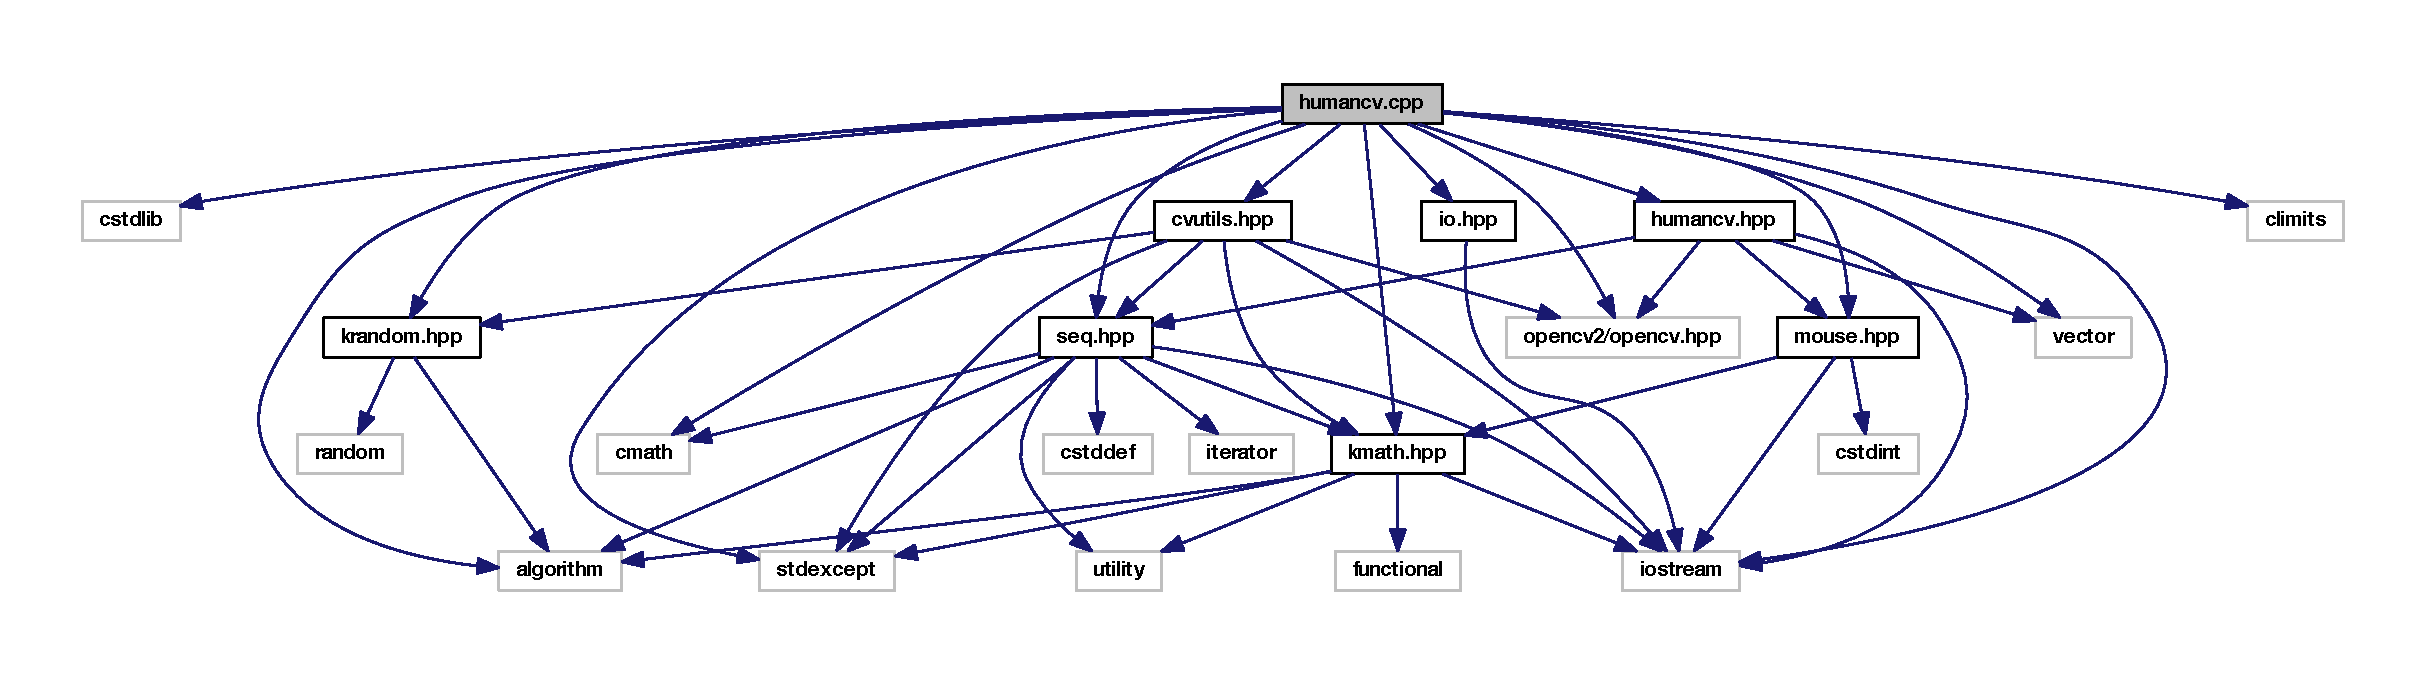
\includegraphics[width=350pt]{humancv_8cpp__incl}
\end{center}
\end{figure}
\subsection*{Functions}
\begin{DoxyCompactItemize}
\item 
ostream \& \hyperlink{humancv_8cpp_a6341d1d30d8b360b043084bd59b601ea}{operator$<$$<$} (ostream \&out, const \hyperlink{structhumancv_1_1_finger_data}{Finger\-Data} \&f)
\item 
\hyperlink{humancv_8cpp_a17e0538341040ddcd8191df955bee277}{thres} (0)
\item 
\hyperlink{humancv_8cpp_a8a980fb3e7af94e18a51575e5f674153}{k\-Filter} (4, 2, 0)
\item 
\hyperlink{humancv_8cpp_aaba9cbcce4c721b4413f3668ba6dced0}{screen\-Rect} (\hyperlink{humancv_8cpp_aaba9cbcce4c721b4413f3668ba6dced0}{screen\-Rect})
\item 
\hyperlink{humancv_8cpp_a6281217d4d46229c11711889d958e4f3}{mouse\-Rect} (\hyperlink{humancv_8cpp_a6281217d4d46229c11711889d958e4f3}{mouse\-Rect})
\end{DoxyCompactItemize}


\subsection{Function Documentation}
\hypertarget{humancv_8cpp_a6341d1d30d8b360b043084bd59b601ea}{\index{humancv.\-cpp@{humancv.\-cpp}!operator$<$$<$@{operator$<$$<$}}
\index{operator$<$$<$@{operator$<$$<$}!humancv.cpp@{humancv.\-cpp}}
\subsubsection[{operator$<$$<$}]{\setlength{\rightskip}{0pt plus 5cm}ostream\& operator$<$$<$ (
\begin{DoxyParamCaption}
\item[{ostream \&}]{out, }
\item[{const {\bf Finger\-Data} \&}]{f}
\end{DoxyParamCaption}
)}}\label{humancv_8cpp_a6341d1d30d8b360b043084bd59b601ea}
\hypertarget{humancv_8cpp_a17e0538341040ddcd8191df955bee277}{\index{humancv.\-cpp@{humancv.\-cpp}!thres@{thres}}
\index{thres@{thres}!humancv.cpp@{humancv.\-cpp}}
\subsubsection[{thres}]{\setlength{\rightskip}{0pt plus 5cm}{\bf thres} (
\begin{DoxyParamCaption}
\item[{0}]{}
\end{DoxyParamCaption}
)}}\label{humancv_8cpp_a17e0538341040ddcd8191df955bee277}
\hypertarget{humancv_8cpp_a8a980fb3e7af94e18a51575e5f674153}{\index{humancv.\-cpp@{humancv.\-cpp}!k\-Filter@{k\-Filter}}
\index{k\-Filter@{k\-Filter}!humancv.cpp@{humancv.\-cpp}}
\subsubsection[{k\-Filter}]{\setlength{\rightskip}{0pt plus 5cm}{\bf k\-Filter} (
\begin{DoxyParamCaption}
\item[{4}]{, }
\item[{2}]{, }
\item[{0}]{}
\end{DoxyParamCaption}
)}}\label{humancv_8cpp_a8a980fb3e7af94e18a51575e5f674153}
\hypertarget{humancv_8cpp_aaba9cbcce4c721b4413f3668ba6dced0}{\index{humancv.\-cpp@{humancv.\-cpp}!screen\-Rect@{screen\-Rect}}
\index{screen\-Rect@{screen\-Rect}!humancv.cpp@{humancv.\-cpp}}
\subsubsection[{screen\-Rect}]{\setlength{\rightskip}{0pt plus 5cm}{\bf screen\-Rect} (
\begin{DoxyParamCaption}
\item[{{\bf screen\-Rect}}]{}
\end{DoxyParamCaption}
)}}\label{humancv_8cpp_aaba9cbcce4c721b4413f3668ba6dced0}
\hypertarget{humancv_8cpp_a6281217d4d46229c11711889d958e4f3}{\index{humancv.\-cpp@{humancv.\-cpp}!mouse\-Rect@{mouse\-Rect}}
\index{mouse\-Rect@{mouse\-Rect}!humancv.cpp@{humancv.\-cpp}}
\subsubsection[{mouse\-Rect}]{\setlength{\rightskip}{0pt plus 5cm}{\bf mouse\-Rect} (
\begin{DoxyParamCaption}
\item[{{\bf mouse\-Rect}}]{}
\end{DoxyParamCaption}
)}}\label{humancv_8cpp_a6281217d4d46229c11711889d958e4f3}

\hypertarget{humancv_8hpp}{\section{humancv.\-hpp File Reference}
\label{humancv_8hpp}\index{humancv.\-hpp@{humancv.\-hpp}}
}
{\ttfamily \#include $<$iostream$>$}\\*
{\ttfamily \#include $<$vector$>$}\\*
{\ttfamily \#include $<$opencv2/opencv.\-hpp$>$}\\*
{\ttfamily \#include \char`\"{}seq.\-hpp\char`\"{}}\\*
{\ttfamily \#include \char`\"{}mouse.\-hpp\char`\"{}}\\*
Include dependency graph for humancv.\-hpp\-:
\nopagebreak
\begin{figure}[H]
\begin{center}
\leavevmode
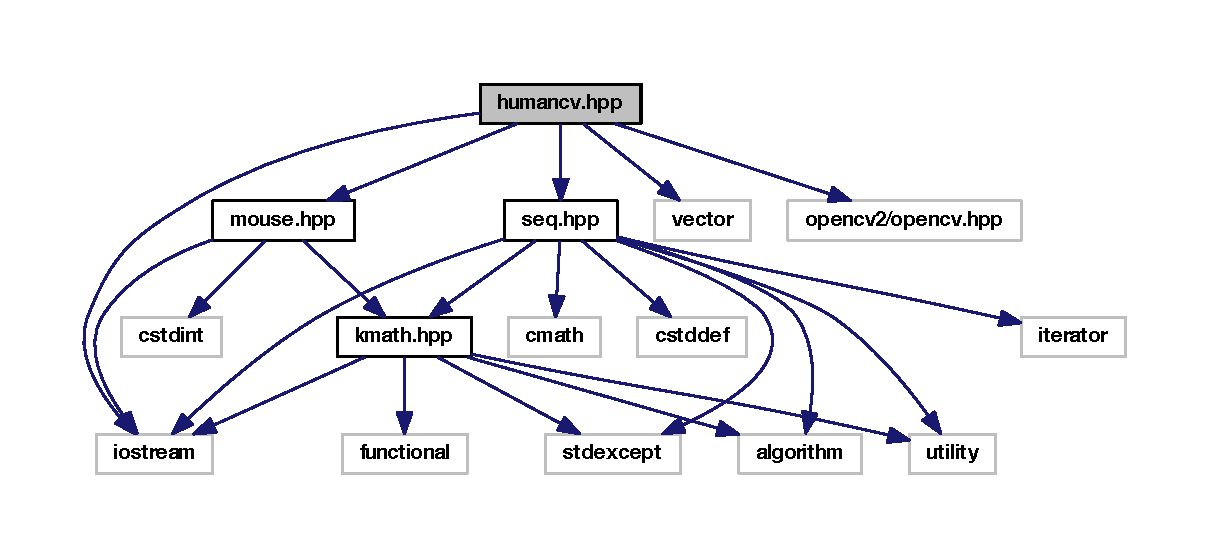
\includegraphics[width=350pt]{humancv_8hpp__incl}
\end{center}
\end{figure}
This graph shows which files directly or indirectly include this file\-:
\nopagebreak
\begin{figure}[H]
\begin{center}
\leavevmode
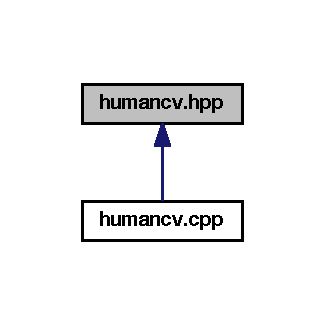
\includegraphics[width=156pt]{humancv_8hpp__dep__incl}
\end{center}
\end{figure}
\subsection*{Classes}
\begin{DoxyCompactItemize}
\item 
struct \hyperlink{structhumancv_1_1_finger_data}{humancv\-::\-Finger\-Data}
\begin{DoxyCompactList}\small\item\em Indices into a {\ttfamily Contour} denoting a finger. \end{DoxyCompactList}\item 
class \hyperlink{classhumancv_1_1_cursor_finder}{humancv\-::\-Cursor\-Finder}
\begin{DoxyCompactList}\small\item\em Framework for tracking hand gestures. \end{DoxyCompactList}\end{DoxyCompactItemize}
\subsection*{Namespaces}
\begin{DoxyCompactItemize}
\item 
namespace \hyperlink{namespacehumancv}{humancv}
\begin{DoxyCompactList}\small\item\em Human-\/related computer vision utilities. \end{DoxyCompactList}\item 
namespace \hyperlink{namespacehumancv_1_1face}{humancv\-::face}
\begin{DoxyCompactList}\small\item\em Basic face detection and modeling. \end{DoxyCompactList}\item 
namespace \hyperlink{namespacehumancv_1_1skin}{humancv\-::skin}
\begin{DoxyCompactList}\small\item\em Color-\/based skin segmentation. \end{DoxyCompactList}\end{DoxyCompactItemize}
\subsection*{Typedefs}
\begin{DoxyCompactItemize}
\item 
typedef \hyperlink{structseq_1_1_wrapped_seq}{seq\-::\-Wrapped\-Seq}\\*
$<$ vector$<$ cv\-::\-Point $>$ $>$ \hyperlink{namespacehumancv_ac3621cda88df26d2718f6bd5ec4de1dd}{humancv\-::\-Contour}
\begin{DoxyCompactList}\small\item\em Since contours are actually \char`\"{}ring\char`\"{} structures but are represented as {\ttfamily vector}s in Open\-C\-V, we wrap them so that indices wrap around. \end{DoxyCompactList}\end{DoxyCompactItemize}
\subsection*{Functions}
\begin{DoxyCompactItemize}
\item 
void \hyperlink{namespacehumancv_aa7c8371defc1384bddefbe8daba81ae9}{humancv\-::get\-Fingers} (const Contour \&ctr, const cv\-::\-Size \&hand\-Size, vector$<$ Finger\-Data $>$ \&out, int k, float min\-Dist, float finger\-Angle=1.\-0)
\begin{DoxyCompactList}\small\item\em Store finger data from a {\ttfamily Contour} representing a hand (with possible arm attached). \end{DoxyCompactList}\item 
void \hyperlink{namespacehumancv_1_1face_a58c6c6dc7819af9f31bebf046ab64ee1}{humancv\-::face\-::store\-Masks} (const cv\-::\-Size im\-Size, const vector$<$ cv\-::\-Rect $>$ \&rois, cv\-::\-Mat\-\_\-$<$ uchar $>$ \&dest)
\begin{DoxyCompactList}\small\item\em Given rectangles containing face and the size of the parent image, store face skin masks in dest of size {\ttfamily im\-Size}. \end{DoxyCompactList}\item 
void \hyperlink{namespacehumancv_1_1face_a6d23e6d95e0f09e1be2b531c75913577}{humancv\-::face\-::get\-Rects} (const cv\-::\-Mat\-\_\-$<$ uchar $>$ \&im, cv\-::\-Cascade\-Classifier \&cascade, vector$<$ cv\-::\-Rect $>$ \&out, float scale=1)
\begin{DoxyCompactList}\small\item\em Store rectangles containing faces in {\ttfamily out}. \end{DoxyCompactList}\item 
void \hyperlink{namespacehumancv_1_1skin_a310ce17c9746ffbb85f230592b41094c}{humancv\-::skin\-::get\-Mask} (const cv\-::\-Mat\-\_\-$<$ cv\-::\-Vec3b $>$ \&im, const Cv\-Boost \&cls, cv\-::\-Mat\-\_\-$<$ uchar $>$ \&dest, cv\-::\-Sparse\-Mat\-\_\-$<$ float $>$ $\ast$lookup=N\-U\-L\-L, float \hyperlink{humancv_8cpp_a17e0538341040ddcd8191df955bee277}{thres}=0)
\begin{DoxyCompactList}\small\item\em Store a binary mask with skin pixels = 255, non-\/skin pixels = 0. \end{DoxyCompactList}\end{DoxyCompactItemize}

\hypertarget{io_8hpp}{\section{io.\-hpp File Reference}
\label{io_8hpp}\index{io.\-hpp@{io.\-hpp}}
}
{\ttfamily \#include $<$iostream$>$}\\*
Include dependency graph for io.\-hpp\-:
\nopagebreak
\begin{figure}[H]
\begin{center}
\leavevmode
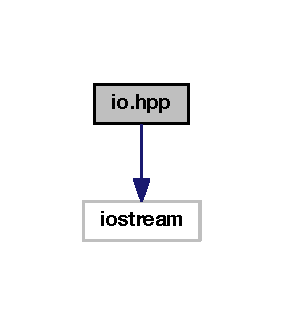
\includegraphics[width=136pt]{io_8hpp__incl}
\end{center}
\end{figure}
This graph shows which files directly or indirectly include this file\-:
\nopagebreak
\begin{figure}[H]
\begin{center}
\leavevmode
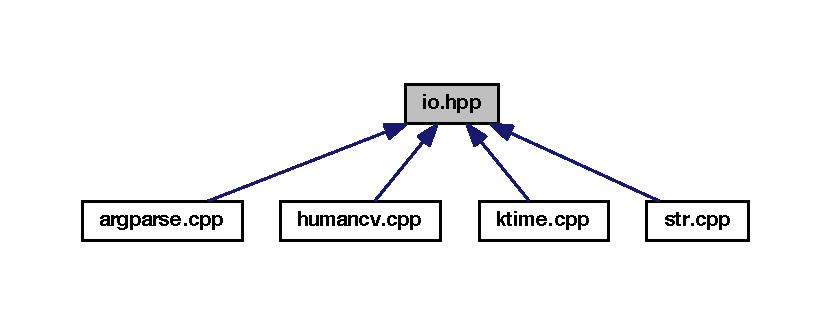
\includegraphics[width=350pt]{io_8hpp__dep__incl}
\end{center}
\end{figure}
\subsection*{Namespaces}
\begin{DoxyCompactItemize}
\item 
namespace \hyperlink{namespaceio}{io}
\begin{DoxyCompactList}\small\item\em Convenience functions for printing values. \end{DoxyCompactList}\end{DoxyCompactItemize}
\subsection*{Functions}
\begin{DoxyCompactItemize}
\item 
{\footnotesize template$<$typename T1 , typename T2 $>$ }\\ostream \& \hyperlink{io_8hpp_a932f5ab08815fcdc72f2866b0d6e1ee2}{operator$<$$<$} (ostream \&out, const pair$<$ T1, T2 $>$ \&p)
\begin{DoxyCompactList}\small\item\em Print a {\ttfamily pair}. \end{DoxyCompactList}\item 
void \hyperlink{namespaceio_ad8499487f5202220fead59833138f4ab}{io\-::print} ()
\begin{DoxyCompactList}\small\item\em Simply print a newline. \end{DoxyCompactList}\item 
{\footnotesize template$<$typename T , typename... Args$>$ }\\void \hyperlink{namespaceio_ab9528b2fe57a002bb153f1b9f8dde743}{io\-::print} (T value, Args...\-args)
\begin{DoxyCompactList}\small\item\em Print arguments separated by spaces, then a newline. \end{DoxyCompactList}\item 
void \hyperlink{namespaceio_ae85db8edfd95c17427c2606360bb97af}{io\-::print\-Imm} ()
\begin{DoxyCompactList}\small\item\em Call {\ttfamily fflush(stdout);}. \end{DoxyCompactList}\item 
{\footnotesize template$<$typename T , typename... Args$>$ }\\void \hyperlink{namespaceio_ade4f05edb2cd007404540f67d416bd4a}{io\-::print\-Imm} (T value, Args...\-args)
\begin{DoxyCompactList}\small\item\em Print arguments separated by spaces with no newline (by default values only show up on the screen when a newline is printed). \end{DoxyCompactList}\end{DoxyCompactItemize}


\subsection{Function Documentation}
\hypertarget{io_8hpp_a932f5ab08815fcdc72f2866b0d6e1ee2}{\index{io.\-hpp@{io.\-hpp}!operator$<$$<$@{operator$<$$<$}}
\index{operator$<$$<$@{operator$<$$<$}!io.hpp@{io.\-hpp}}
\subsubsection[{operator$<$$<$}]{\setlength{\rightskip}{0pt plus 5cm}template$<$typename T1 , typename T2 $>$ ostream\& operator$<$$<$ (
\begin{DoxyParamCaption}
\item[{ostream \&}]{out, }
\item[{const pair$<$ T1, T2 $>$ \&}]{p}
\end{DoxyParamCaption}
)}}\label{io_8hpp_a932f5ab08815fcdc72f2866b0d6e1ee2}


Print a {\ttfamily pair}. 


\hypertarget{kmath_8cpp}{\section{kmath.\-cpp File Reference}
\label{kmath_8cpp}\index{kmath.\-cpp@{kmath.\-cpp}}
}
{\ttfamily \#include $<$cmath$>$}\\*
{\ttfamily \#include $<$stdexcept$>$}\\*
{\ttfamily \#include \char`\"{}kmath.\-hpp\char`\"{}}\\*
Include dependency graph for kmath.\-cpp\-:
\nopagebreak
\begin{figure}[H]
\begin{center}
\leavevmode
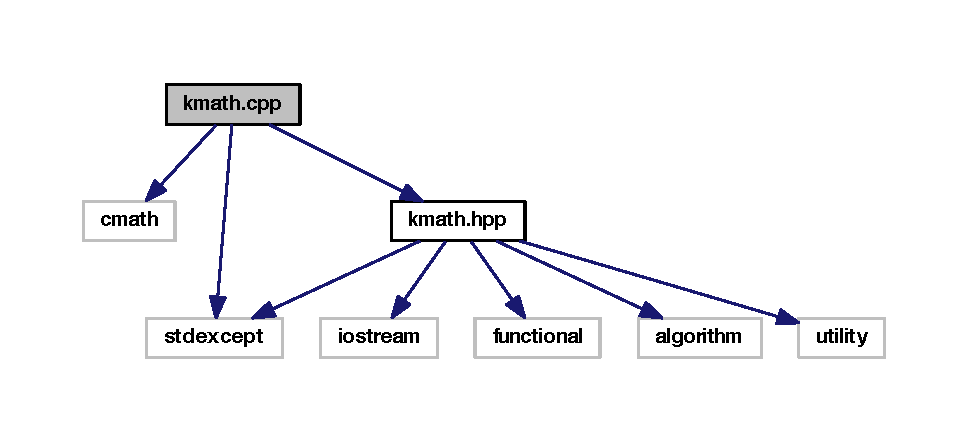
\includegraphics[width=350pt]{kmath_8cpp__incl}
\end{center}
\end{figure}

\hypertarget{kmath_8hpp}{\section{kmath.\-hpp File Reference}
\label{kmath_8hpp}\index{kmath.\-hpp@{kmath.\-hpp}}
}
{\ttfamily \#include $<$iostream$>$}\\*
{\ttfamily \#include $<$stdexcept$>$}\\*
{\ttfamily \#include $<$functional$>$}\\*
{\ttfamily \#include $<$algorithm$>$}\\*
{\ttfamily \#include $<$utility$>$}\\*
Include dependency graph for kmath.\-hpp\-:\nopagebreak
\begin{figure}[H]
\begin{center}
\leavevmode
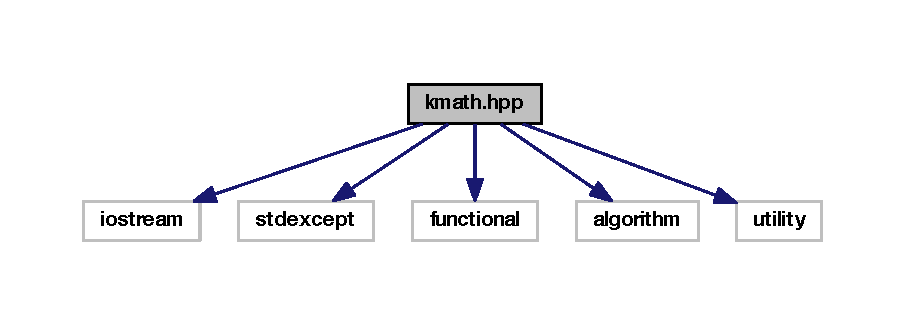
\includegraphics[width=350pt]{kmath_8hpp__incl}
\end{center}
\end{figure}
This graph shows which files directly or indirectly include this file\-:
\nopagebreak
\begin{figure}[H]
\begin{center}
\leavevmode
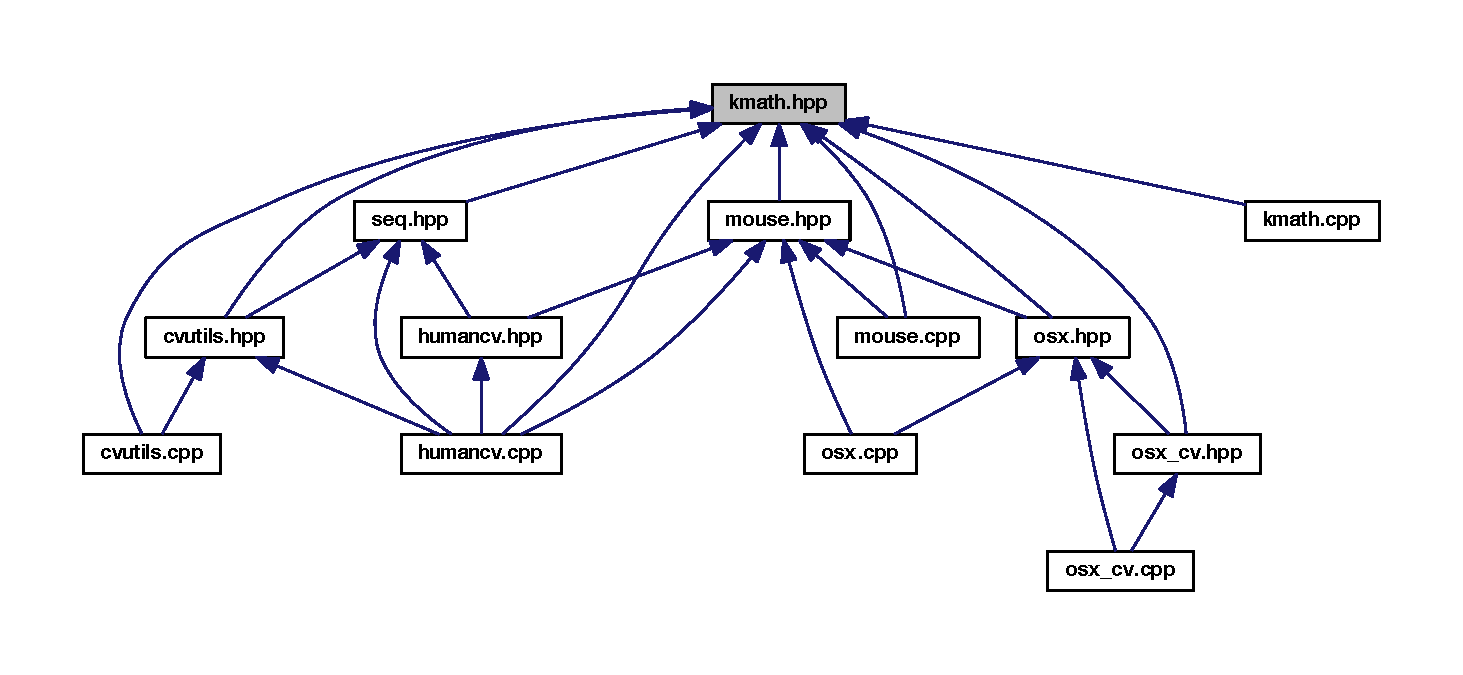
\includegraphics[width=350pt]{kmath_8hpp__dep__incl}
\end{center}
\end{figure}
\subsection*{Classes}
\begin{DoxyCompactItemize}
\item 
struct \hyperlink{structkmath_1_1_point}{kmath\-::\-Point$<$ T $>$}
\begin{DoxyCompactList}\small\item\em Generic point class. \end{DoxyCompactList}\item 
struct \hyperlink{structkmath_1_1_interval}{kmath\-::\-Interval}
\begin{DoxyCompactList}\small\item\em Represents an interval of real numbers. \end{DoxyCompactList}\end{DoxyCompactItemize}
\subsection*{Namespaces}
\begin{DoxyCompactItemize}
\item 
namespace \hyperlink{namespacekmath}{kmath}
\begin{DoxyCompactList}\small\item\em Miscellaneous mathematical functions. \end{DoxyCompactList}\end{DoxyCompactItemize}
\subsection*{Typedefs}
\begin{DoxyCompactItemize}
\item 
typedef Point$<$ int $>$ \hyperlink{namespacekmath_afaf3fde3b20c9932e144eb48e736cad9}{kmath\-::\-Point\-I}
\item 
typedef Point$<$ float $>$ \hyperlink{namespacekmath_ad80aa80b21a1aeadbd484a0fc56f4e95}{kmath\-::\-Point\-F}
\item 
typedef Point$<$ double $>$ \hyperlink{namespacekmath_aad2e627ee7da1b98c2c516f20ed5b7e3}{kmath\-::\-Point\-D}
\end{DoxyCompactItemize}
\subsection*{Enumerations}
\begin{DoxyCompactItemize}
\item 
enum \hyperlink{namespacekmath_a1e00ae34fe8ed9548870fc759ea82609}{kmath\-::\-Round\-Type} \{ \hyperlink{namespacekmath_a1e00ae34fe8ed9548870fc759ea82609ae04658d947a7879a4502f837c286f1ac}{kmath\-::\-R\-O\-U\-N\-D}, 
\hyperlink{namespacekmath_a1e00ae34fe8ed9548870fc759ea82609a449ece60a17b2668fdb165fd8740dbdf}{kmath\-::\-C\-E\-I\-L}, 
\hyperlink{namespacekmath_a1e00ae34fe8ed9548870fc759ea82609a8f67a6160bf7ac646e9b1bb6ef1a56c1}{kmath\-::\-F\-L\-O\-O\-R}
 \}
\begin{DoxyCompactList}\small\item\em Type of rounding to do, used in \hyperlink{namespacekmath_aa18b5fc52315b0ca7717a52bdf152ee6}{fround()}. \end{DoxyCompactList}\end{DoxyCompactItemize}
\subsection*{Functions}
\begin{DoxyCompactItemize}
\item 
{\footnotesize template$<$typename T $>$ }\\int \hyperlink{namespacekmath_a1e0f4e049ef1ec26bf84a8aa77f067d1}{kmath\-::sgn} (T val)
\begin{DoxyCompactList}\small\item\em Return 1 if {\ttfamily val} $>$ 0, -\/1 if {\ttfamily val} $<$ 0, or 0 if {\ttfamily val} == 0. \end{DoxyCompactList}\item 
{\footnotesize template$<$$>$ }\\int \hyperlink{namespacekmath_af5735a3b3983474d19d1a982a26cb473}{kmath\-::sgn} (unsigned val)
\begin{DoxyCompactList}\small\item\em Specialization for unsigned types. \end{DoxyCompactList}\item 
{\footnotesize template$<$$>$ }\\int \hyperlink{namespacekmath_a7308728815e450bfe583078b893afd2b}{kmath\-::sgn} (unsigned long val)
\begin{DoxyCompactList}\small\item\em Specialization for unsigned types. \end{DoxyCompactList}\item 
{\footnotesize template$<$$>$ }\\int \hyperlink{namespacekmath_a06e8ca1a174b7eb44ba4ffdebbdf0179}{kmath\-::sgn} (unsigned long long val)
\begin{DoxyCompactList}\small\item\em Specialization for unsigned types. \end{DoxyCompactList}\item 
double \hyperlink{namespacekmath_ac9d0f66e32f84c22626883c171893f48}{kmath\-::normal\-C\-D\-F} (double x)
\begin{DoxyCompactList}\small\item\em Return the cumulative density of a Gaussian distribution with mean = 0, variance = 1. \end{DoxyCompactList}\item 
unsigned \hyperlink{namespacekmath_abfda38c9ce9a9d07af7f93a731d8fe51}{kmath\-::factorial} (unsigned n)
\begin{DoxyCompactList}\small\item\em Return {\ttfamily n!}. \end{DoxyCompactList}\item 
unsigned \hyperlink{namespacekmath_a53519d2ec30d9df038dbe8ceaead1a9c}{kmath\-::combinations} (unsigned n, unsigned k)
\begin{DoxyCompactList}\small\item\em Return $_{\mbox{n}}$ C$_{\mbox{k}}$  (n choose k). \end{DoxyCompactList}\item 
float \hyperlink{namespacekmath_aa18b5fc52315b0ca7717a52bdf152ee6}{kmath\-::fround} (float val, float scale=1.\-0, \hyperlink{namespacekmath_a1e00ae34fe8ed9548870fc759ea82609}{Round\-Type} action=R\-O\-U\-N\-D)
\begin{DoxyCompactList}\small\item\em Round val to nearest multiple of scale. \end{DoxyCompactList}\item 
int \hyperlink{namespacekmath_a32d7d4c091092ac7e21d7beb15daaf1a}{kmath\-::iround} (float val)
\begin{DoxyCompactList}\small\item\em Specialization of {\ttfamily fround} that rounds float to nearest integer. \end{DoxyCompactList}\item 
float \hyperlink{namespacekmath_a1792feb5272baa371047829dc4a30264}{kmath\-::interval\-Project} (float val, const Interval \&domain, const Interval \&range, const function$<$ float(float)$>$ \&func=\mbox{[}$\,$\mbox{]}(float x)\{return x;\}, const Interval \&func\-Domain=Interval(0, 1), const Interval \&func\-Range=Interval(0, 1), bool bound=true)
\begin{DoxyCompactList}\small\item\em Project a value within {\ttfamily domain} to a new interval {\ttfamily range} using {\ttfamily func}. \end{DoxyCompactList}\end{DoxyCompactItemize}
\subsection*{Variables}
\begin{DoxyCompactItemize}
\item 
const double \hyperlink{namespacekmath_a1224c45abb03af2a5136e24f09d9b4c3}{kmath\-::\-P\-I} = 3.\-141592654
\begin{DoxyCompactList}\small\item\em The ratio of the circumference of a circle to its diameter. \end{DoxyCompactList}\end{DoxyCompactItemize}

\hypertarget{krandom_8cpp}{\section{krandom.\-cpp File Reference}
\label{krandom_8cpp}\index{krandom.\-cpp@{krandom.\-cpp}}
}
{\ttfamily \#include $<$random$>$}\\*
{\ttfamily \#include \char`\"{}krandom.\-hpp\char`\"{}}\\*
Include dependency graph for krandom.\-cpp\-:
\nopagebreak
\begin{figure}[H]
\begin{center}
\leavevmode
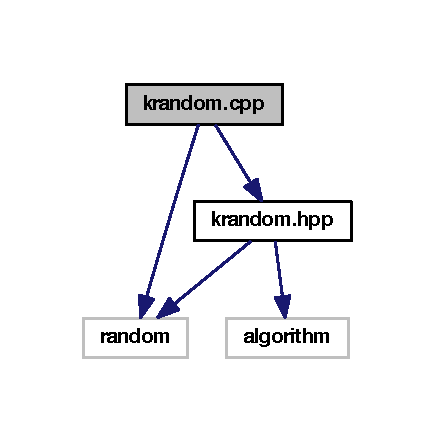
\includegraphics[width=208pt]{krandom_8cpp__incl}
\end{center}
\end{figure}
\subsection*{Functions}
\begin{DoxyCompactItemize}
\item 
vector$<$ unsigned $>$ \hyperlink{krandom_8cpp_a55dd773165033113e7e200186d6e88ad}{get\-Sample\-Inds} (unsigned pop\-Size, unsigned samp\-Size, bool with\-Replacement)
\end{DoxyCompactItemize}


\subsection{Function Documentation}
\hypertarget{krandom_8cpp_a55dd773165033113e7e200186d6e88ad}{\index{krandom.\-cpp@{krandom.\-cpp}!get\-Sample\-Inds@{get\-Sample\-Inds}}
\index{get\-Sample\-Inds@{get\-Sample\-Inds}!krandom.cpp@{krandom.\-cpp}}
\subsubsection[{get\-Sample\-Inds}]{\setlength{\rightskip}{0pt plus 5cm}vector$<$unsigned$>$ {\bf get\-Sample\-Inds} (
\begin{DoxyParamCaption}
\item[{unsigned}]{pop\-Size, }
\item[{unsigned}]{samp\-Size, }
\item[{bool}]{with\-Replacement}
\end{DoxyParamCaption}
)}}\label{krandom_8cpp_a55dd773165033113e7e200186d6e88ad}

\hypertarget{krandom_8hpp}{\section{krandom.\-hpp File Reference}
\label{krandom_8hpp}\index{krandom.\-hpp@{krandom.\-hpp}}
}
{\ttfamily \#include $<$random$>$}\\*
{\ttfamily \#include $<$algorithm$>$}\\*
\subsection*{Namespaces}
\begin{DoxyCompactItemize}
\item 
namespace \hyperlink{namespacekrandom}{krandom}
\begin{DoxyCompactList}\small\item\em Simple wrapper around {\ttfamily $<$random$>$} with a Python interface. \end{DoxyCompactList}\end{DoxyCompactItemize}
\subsection*{Functions}
\begin{DoxyCompactItemize}
\item 
int \hyperlink{namespacekrandom_a32b7337c1131ea0fbbd6b5f20aac2002}{krandom\-::randint} (int low, int high)
\item 
long \hyperlink{namespacekrandom_adc8e2bfa37c40fdecc8f601a266ab447}{krandom\-::randint} (long low, long high)
\item 
long long \hyperlink{namespacekrandom_a4672262133b6b130d7ca8b49f55595a2}{krandom\-::randint} (long long low, long long high)
\item 
double \hyperlink{namespacekrandom_a6a320147afafc7e81429b1a1ab4ec2e0}{krandom\-::random} ()
\item 
float \hyperlink{namespacekrandom_aa5f77704c3bf39731c986b7d27caf0fe}{krandom\-::uniform} (float low, float high)
\item 
double \hyperlink{namespacekrandom_ae89a756b3d067650aa9712efe6e930e2}{krandom\-::uniform} (double low, double high)
\item 
{\footnotesize template$<$class Iter\-Type $>$ }\\void \hyperlink{namespacekrandom_abac374525fd029faa58cb9c43cab41eb}{krandom\-::shuffle} (Iter\-Type start, Iter\-Type end)
\item 
{\footnotesize template$<$class Seq\-Type $>$ }\\void \hyperlink{namespacekrandom_a3cf920703fa6e180b1aa4d4c86799626}{krandom\-::shuffle} (Seq\-Type \&seq)
\item 
{\footnotesize template$<$template$<$ typename U, typename...\-Args $>$ class Seq\-Type, typename Item\-Type $>$ }\\Item\-Type \hyperlink{namespacekrandom_a59c038687d5825d1b6b8f26cf91dee20}{krandom\-::choice} (const Seq\-Type$<$ Item\-Type $>$ \&seq)
\item 
vector$<$ unsigned $>$ \& \hyperlink{namespacekrandom_a50015c42a5cb2ab60017b00abbb4ffde}{krandom\-::get\-Sample\-Inds} (unsigned pop\-Size, unsigned samp\-Size, vector$<$ unsigned $>$ \&inds, bool with\-Replacement=true)
\item 
vector$<$ unsigned $>$ \hyperlink{namespacekrandom_aa1ecb85e031f5505020d74732acd846a}{krandom\-::get\-Sample\-Inds} (unsigned pop\-Size, unsigned samp\-Size, bool with\-Replacement=true)
\item 
{\footnotesize template$<$typename Seq\-Type $>$ }\\void \hyperlink{namespacekrandom_a924f7dd5ed9785fd396615b9995e47da}{krandom\-::sample} (const Seq\-Type \&seq, unsigned samp\-Size, Seq\-Type \&out, bool with\-Replacement=true)
\item 
{\footnotesize template$<$typename Seq\-Type $>$ }\\Seq\-Type \hyperlink{namespacekrandom_a59cee8cdbf9ac39cc5d3762935dbdfb7}{krandom\-::sample} (const Seq\-Type \&seq, unsigned samp\-Size, bool with\-Replacement=true)
\end{DoxyCompactItemize}
\subsection*{Variables}
\begin{DoxyCompactItemize}
\item 
random\-\_\-device \hyperlink{namespacekrandom_a5c40b80390a0425475af691519056f21}{krandom\-::engine}
\end{DoxyCompactItemize}

\hypertarget{ktime_8cpp}{\section{ktime.\-cpp File Reference}
\label{ktime_8cpp}\index{ktime.\-cpp@{ktime.\-cpp}}
}
{\ttfamily \#include \char`\"{}ktime.\-hpp\char`\"{}}\\*
{\ttfamily \#include \char`\"{}io.\-hpp\char`\"{}}\\*

\hypertarget{ktime_8hpp}{\section{ktime.\-hpp File Reference}
\label{ktime_8hpp}\index{ktime.\-hpp@{ktime.\-hpp}}
}
{\ttfamily \#include $<$queue$>$}\\*
{\ttfamily \#include $<$chrono$>$}\\*
\subsection*{Classes}
\begin{DoxyCompactItemize}
\item 
class \hyperlink{classktime_1_1_running_avg_timer}{ktime\-::\-Running\-Avg\-Timer}
\end{DoxyCompactItemize}
\subsection*{Namespaces}
\begin{DoxyCompactItemize}
\item 
namespace \hyperlink{namespacektime}{ktime}
\begin{DoxyCompactList}\small\item\em Utilities for working with time. \end{DoxyCompactList}\end{DoxyCompactItemize}
\subsection*{Typedefs}
\begin{DoxyCompactItemize}
\item 
typedef chrono\-::system\-\_\-clock \hyperlink{namespacektime_ac6b33ea027bdc032e7ba377509c8e51f}{ktime\-::\-Clock\-T}
\item 
typedef Clock\-T\-::duration \hyperlink{namespacektime_aacefffdcc0ccc2f45598475b3557d6f2}{ktime\-::\-Time\-Diff}
\item 
typedef Clock\-T\-::time\-\_\-point \hyperlink{namespacektime_a038a3d1fb2cb9885396233d6e412773e}{ktime\-::\-Time\-Point}
\end{DoxyCompactItemize}
\subsection*{Functions}
\begin{DoxyCompactItemize}
\item 
float \hyperlink{namespacektime_a89b89374ae2f385f58b64c5a2438a718}{ktime\-::to\-Secs} (const \hyperlink{namespacektime_aacefffdcc0ccc2f45598475b3557d6f2}{Time\-Diff} \&diff)
\end{DoxyCompactItemize}

\hypertarget{mouse_8cpp}{\section{mouse.\-cpp File Reference}
\label{mouse_8cpp}\index{mouse.\-cpp@{mouse.\-cpp}}
}
{\ttfamily \#include $<$iostream$>$}\\*
{\ttfamily \#include \char`\"{}mouse.\-hpp\char`\"{}}\\*
{\ttfamily \#include \char`\"{}kmath.\-hpp\char`\"{}}\\*
Include dependency graph for mouse.\-cpp\-:
\nopagebreak
\begin{figure}[H]
\begin{center}
\leavevmode
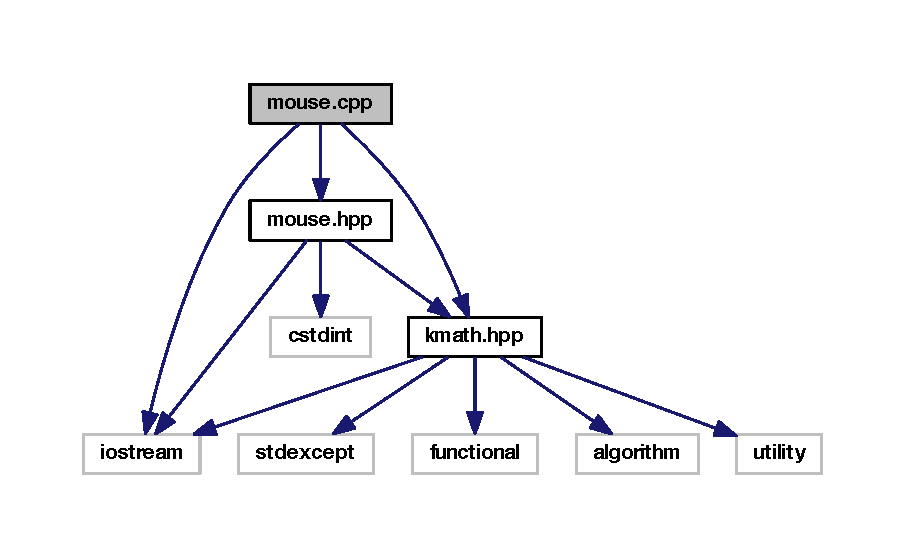
\includegraphics[width=350pt]{mouse_8cpp__incl}
\end{center}
\end{figure}
\subsection*{Functions}
\begin{DoxyCompactItemize}
\item 
ostream \& \hyperlink{mouse_8cpp_ae8bd9d4449a110c93fc82ac06ee625fa}{operator$<$$<$} (ostream \&out, const \hyperlink{structmouse_1_1_state}{mouse\-::\-State} \&m)
\end{DoxyCompactItemize}


\subsection{Function Documentation}
\hypertarget{mouse_8cpp_ae8bd9d4449a110c93fc82ac06ee625fa}{\index{mouse.\-cpp@{mouse.\-cpp}!operator$<$$<$@{operator$<$$<$}}
\index{operator$<$$<$@{operator$<$$<$}!mouse.cpp@{mouse.\-cpp}}
\subsubsection[{operator$<$$<$}]{\setlength{\rightskip}{0pt plus 5cm}ostream\& operator$<$$<$ (
\begin{DoxyParamCaption}
\item[{ostream \&}]{out, }
\item[{const {\bf mouse\-::\-State} \&}]{m}
\end{DoxyParamCaption}
)}}\label{mouse_8cpp_ae8bd9d4449a110c93fc82ac06ee625fa}

\hypertarget{mouse_8hpp}{\section{mouse.\-hpp File Reference}
\label{mouse_8hpp}\index{mouse.\-hpp@{mouse.\-hpp}}
}
{\ttfamily \#include $<$cstdint$>$}\\*
{\ttfamily \#include $<$iostream$>$}\\*
{\ttfamily \#include \char`\"{}kmath.\-hpp\char`\"{}}\\*
Include dependency graph for mouse.\-hpp\-:\nopagebreak
\begin{figure}[H]
\begin{center}
\leavevmode
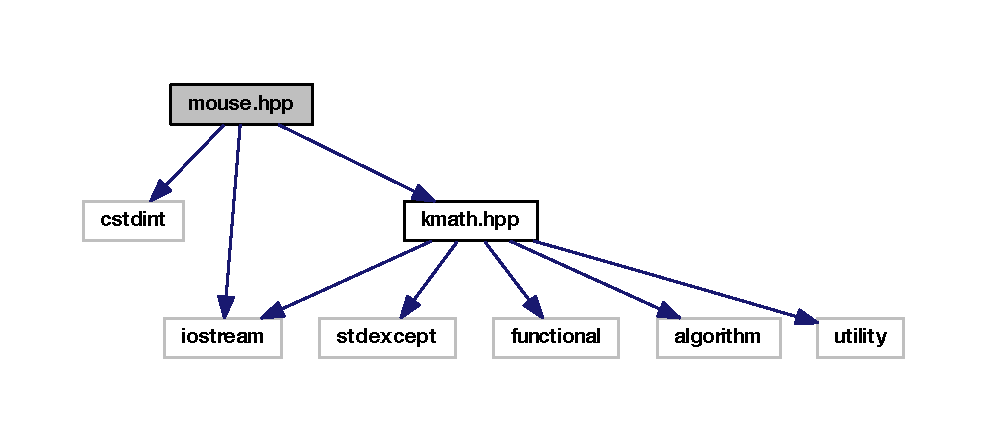
\includegraphics[width=350pt]{mouse_8hpp__incl}
\end{center}
\end{figure}
This graph shows which files directly or indirectly include this file\-:\nopagebreak
\begin{figure}[H]
\begin{center}
\leavevmode
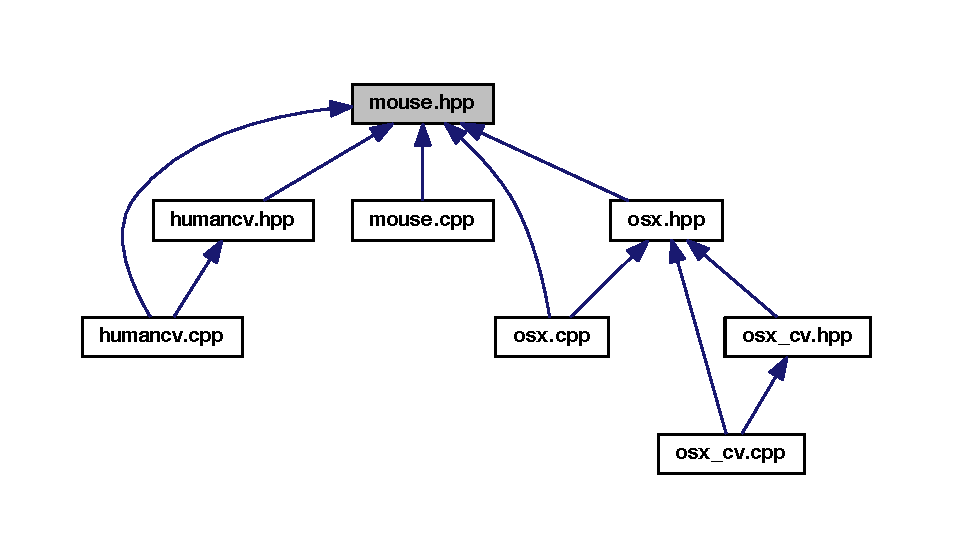
\includegraphics[width=265pt]{mouse_8hpp__dep__incl}
\end{center}
\end{figure}
\subsection*{Classes}
\begin{DoxyCompactItemize}
\item 
struct \hyperlink{structmouse_1_1_state}{mouse\-::\-State}
\begin{DoxyCompactList}\small\item\em Simple data holder for a button flag and a position. \end{DoxyCompactList}\end{DoxyCompactItemize}
\subsection*{Namespaces}
\begin{DoxyCompactItemize}
\item 
namespace \hyperlink{namespacemouse}{mouse}
\begin{DoxyCompactList}\small\item\em Utilities for modeling the mouse state. \end{DoxyCompactList}\end{DoxyCompactItemize}
\subsection*{Enumerations}
\begin{DoxyCompactItemize}
\item 
enum \hyperlink{namespacemouse_af85c842f9410a5f81fe933360fb19bc4}{mouse\-::\-Button} \{ \hyperlink{namespacemouse_af85c842f9410a5f81fe933360fb19bc4ad099c4586c3d6cf30e4d4da38bc414ca}{mouse\-::\-L\-E\-F\-T\-\_\-\-B\-U\-T\-T\-O\-N}, 
\hyperlink{namespacemouse_af85c842f9410a5f81fe933360fb19bc4a9ab944e0c7a1999da316be044705f024}{mouse\-::\-R\-I\-G\-H\-T\-\_\-\-B\-U\-T\-T\-O\-N}
 \}
\end{DoxyCompactItemize}

\hypertarget{osx_8cpp}{\section{osx.\-cpp File Reference}
\label{osx_8cpp}\index{osx.\-cpp@{osx.\-cpp}}
}
{\ttfamily \#include $<$cstdint$>$}\\*
{\ttfamily \#include $<$iostream$>$}\\*
{\ttfamily \#include $<$stdexcept$>$}\\*
{\ttfamily \#include $<$Application\-Services/\-Application\-Services.\-h$>$}\\*
{\ttfamily \#include \char`\"{}osx.\-hpp\char`\"{}}\\*
Include dependency graph for osx.\-cpp\-:\nopagebreak
\begin{figure}[H]
\begin{center}
\leavevmode
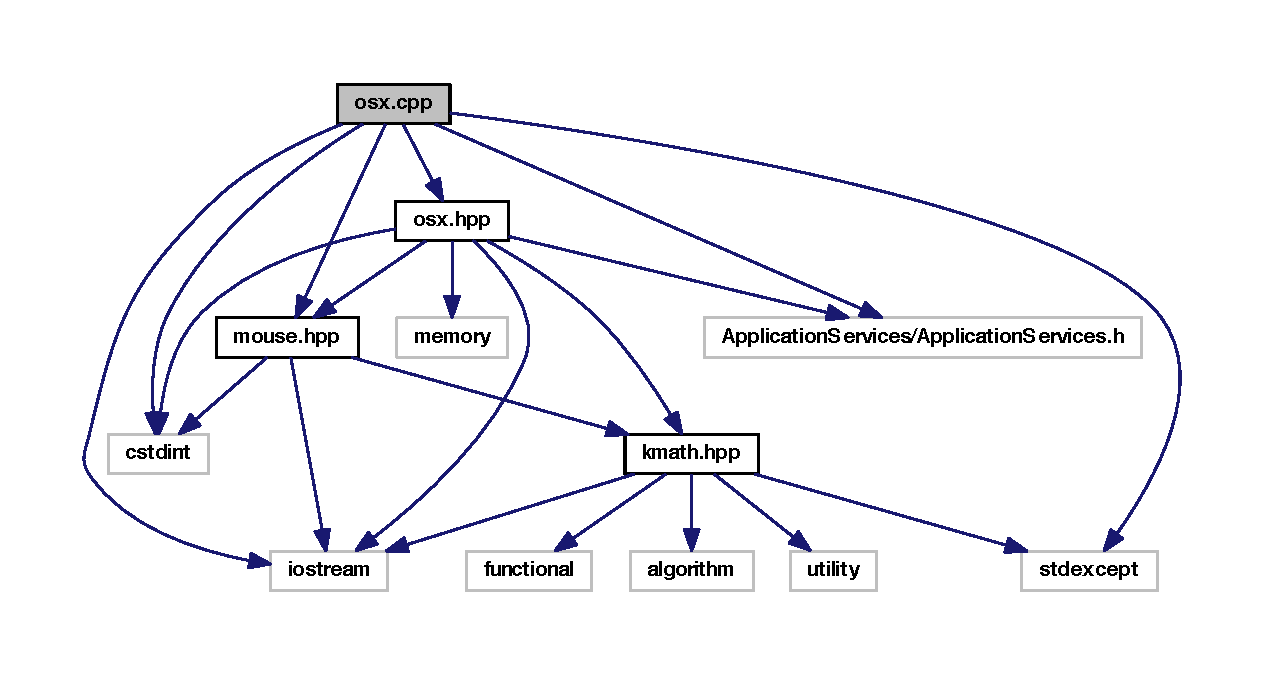
\includegraphics[width=350pt]{osx_8cpp__incl}
\end{center}
\end{figure}
\subsection*{Functions}
\begin{DoxyCompactItemize}
\item 
ostream \& \hyperlink{osx_8cpp_af829f2833c7596fe7b9cf41b58ae29b1}{operator$<$$<$} (ostream \&out, const mouse\-::\-Mouse\-State \&m)
\item 
ostream \& \hyperlink{osx_8cpp_ae35a0729fcf841f08cc4c1cd53038f97}{operator$<$$<$} (ostream \&out, const C\-G\-Color\-Space\-Ref \&color\-Space)
\begin{DoxyCompactList}\small\item\em Print {\ttfamily C\-G\-Color\-Space\-Ref} info. \end{DoxyCompactList}\item 
ostream \& \hyperlink{osx_8cpp_ac2540fce1dc9490db082314832db4a6a}{operator$<$$<$} (ostream \&out, const C\-G\-Image\-Ref \&im\-Ref)
\begin{DoxyCompactList}\small\item\em Print {\ttfamily C\-G\-Image\-Ref} info. \end{DoxyCompactList}\end{DoxyCompactItemize}


\subsection{Function Documentation}
\hypertarget{osx_8cpp_af829f2833c7596fe7b9cf41b58ae29b1}{\index{osx.\-cpp@{osx.\-cpp}!operator$<$$<$@{operator$<$$<$}}
\index{operator$<$$<$@{operator$<$$<$}!osx.cpp@{osx.\-cpp}}
\subsubsection[{operator$<$$<$}]{\setlength{\rightskip}{0pt plus 5cm}ostream\& operator$<$$<$ (
\begin{DoxyParamCaption}
\item[{ostream \&}]{out, }
\item[{const mouse\-::\-Mouse\-State \&}]{m}
\end{DoxyParamCaption}
)}}\label{osx_8cpp_af829f2833c7596fe7b9cf41b58ae29b1}
\hypertarget{osx_8cpp_ae35a0729fcf841f08cc4c1cd53038f97}{\index{osx.\-cpp@{osx.\-cpp}!operator$<$$<$@{operator$<$$<$}}
\index{operator$<$$<$@{operator$<$$<$}!osx.cpp@{osx.\-cpp}}
\subsubsection[{operator$<$$<$}]{\setlength{\rightskip}{0pt plus 5cm}ostream\& operator$<$$<$ (
\begin{DoxyParamCaption}
\item[{ostream \&}]{out, }
\item[{const C\-G\-Color\-Space\-Ref \&}]{color\-Space}
\end{DoxyParamCaption}
)}}\label{osx_8cpp_ae35a0729fcf841f08cc4c1cd53038f97}


Print {\ttfamily C\-G\-Color\-Space\-Ref} info. 

\hypertarget{osx_8cpp_ac2540fce1dc9490db082314832db4a6a}{\index{osx.\-cpp@{osx.\-cpp}!operator$<$$<$@{operator$<$$<$}}
\index{operator$<$$<$@{operator$<$$<$}!osx.cpp@{osx.\-cpp}}
\subsubsection[{operator$<$$<$}]{\setlength{\rightskip}{0pt plus 5cm}ostream\& operator$<$$<$ (
\begin{DoxyParamCaption}
\item[{ostream \&}]{out, }
\item[{const C\-G\-Image\-Ref \&}]{im\-Ref}
\end{DoxyParamCaption}
)}}\label{osx_8cpp_ac2540fce1dc9490db082314832db4a6a}


Print {\ttfamily C\-G\-Image\-Ref} info. 


\hypertarget{osx_8hpp}{\section{osx.\-hpp File Reference}
\label{osx_8hpp}\index{osx.\-hpp@{osx.\-hpp}}
}
{\ttfamily \#include $<$cstdint$>$}\\*
{\ttfamily \#include $<$iostream$>$}\\*
{\ttfamily \#include $<$memory$>$}\\*
{\ttfamily \#include $<$Application\-Services/\-Application\-Services.\-h$>$}\\*
{\ttfamily \#include \char`\"{}mouse.\-hpp\char`\"{}}\\*
{\ttfamily \#include \char`\"{}kmath.\-hpp\char`\"{}}\\*
Include dependency graph for osx.\-hpp\-:
\nopagebreak
\begin{figure}[H]
\begin{center}
\leavevmode
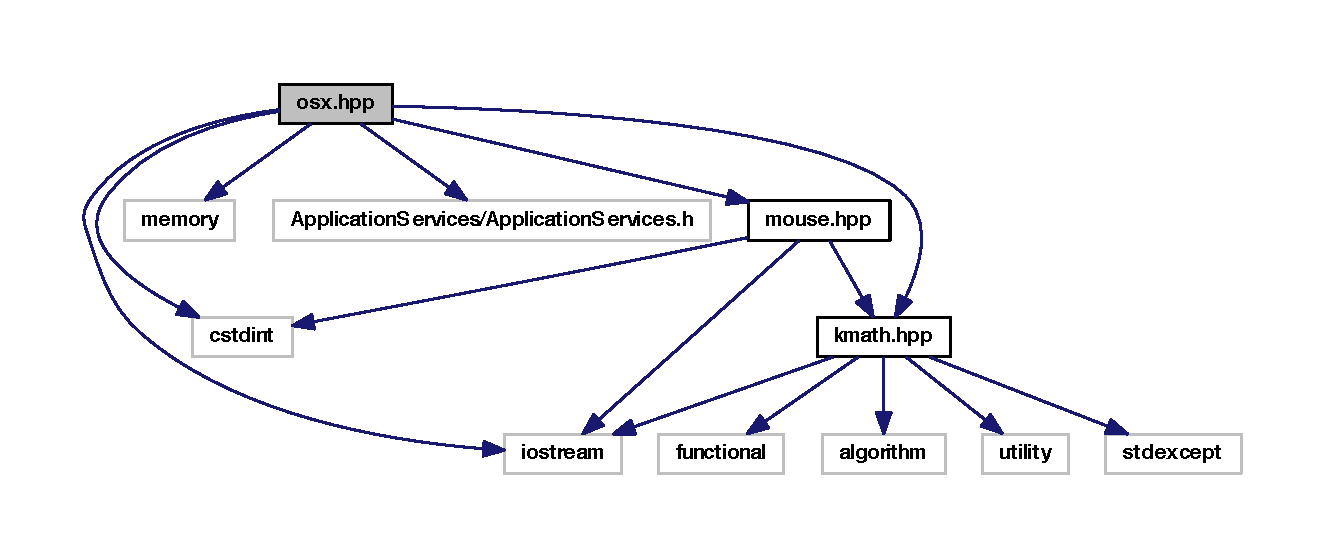
\includegraphics[width=350pt]{osx_8hpp__incl}
\end{center}
\end{figure}
This graph shows which files directly or indirectly include this file\-:\nopagebreak
\begin{figure}[H]
\begin{center}
\leavevmode
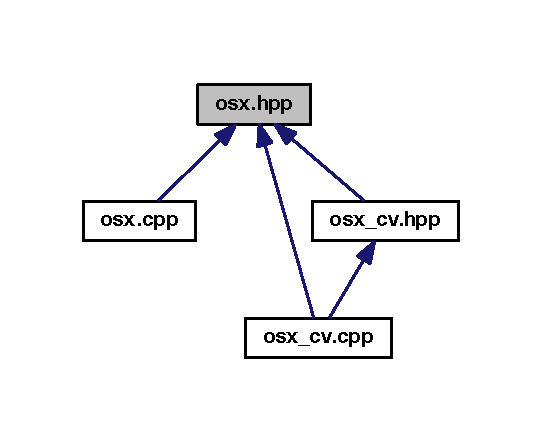
\includegraphics[width=260pt]{osx_8hpp__dep__incl}
\end{center}
\end{figure}
\subsection*{Classes}
\begin{DoxyCompactItemize}
\item 
struct \hyperlink{structosx_1_1disp_1_1_image}{osx\-::disp\-::\-Image}
\begin{DoxyCompactList}\small\item\em Memory-\/managed wrapper aronud {\ttfamily C\-G\-Image\-Ref} using a {\ttfamily shared\-\_\-ptr}. \end{DoxyCompactList}\end{DoxyCompactItemize}
\subsection*{Namespaces}
\begin{DoxyCompactItemize}
\item 
namespace \hyperlink{namespaceosx}{osx}
\begin{DoxyCompactList}\small\item\em O\-S\-X-\/specific utilities. \end{DoxyCompactList}\item 
namespace \hyperlink{namespaceosx_1_1mouse}{osx\-::mouse}
\begin{DoxyCompactList}\small\item\em Utilities for controlling the mouse. \end{DoxyCompactList}\item 
namespace \hyperlink{namespaceosx_1_1disp}{osx\-::disp}
\begin{DoxyCompactList}\small\item\em Functions for extracting the display image. \end{DoxyCompactList}\end{DoxyCompactItemize}
\subsection*{Defines}
\begin{DoxyCompactItemize}
\item 
\#define \hyperlink{osx_8hpp_ac041cfa66801dc389105798b67525f1e}{U\-N\-U\-S\-E\-D\-\_\-\-V\-A\-R}
\end{DoxyCompactItemize}
\subsection*{Enumerations}
\begin{DoxyCompactItemize}
\item 
enum \hyperlink{namespaceosx_1_1disp_a63adf9b0b0b0365ec428dd44fc30c659}{osx\-::disp\-::\-R\-G\-B\-Type} \{ \hyperlink{namespaceosx_1_1disp_a63adf9b0b0b0365ec428dd44fc30c659ab96ecb2ad3c69bf9019d7ed4253603b1}{osx\-::disp\-::\-C\-O\-L\-O\-R\-\_\-\-B\-G\-R}, 
\hyperlink{namespaceosx_1_1disp_a63adf9b0b0b0365ec428dd44fc30c659a307b3e319b6708774c7672d7efc04d0d}{osx\-::disp\-::\-C\-O\-L\-O\-R\-\_\-\-A\-R\-G\-B}, 
\hyperlink{namespaceosx_1_1disp_a63adf9b0b0b0365ec428dd44fc30c659aefca227dbfbf6803b1248aceeaa187b7}{osx\-::disp\-::\-C\-O\-L\-O\-R\-\_\-\-R\-G\-B\-A}
 \}
\end{DoxyCompactItemize}
\subsection*{Functions}
\begin{DoxyCompactItemize}
\item 
{\footnotesize template$<$typename T $>$ }\\C\-G\-Point \hyperlink{namespaceosx_abf7318d332d5e87088a270877f3da1ee}{osx\-::to\-C\-G\-Pt} (\hyperlink{structkmath_1_1_point}{kmath\-::\-Point}$<$ T $>$ pt)
\item 
\hyperlink{namespacekmath_ad80aa80b21a1aeadbd484a0fc56f4e95}{kmath\-::\-Point\-F} \hyperlink{namespaceosx_a37f829bcbe1e218b01dafeb711bd9d42}{osx\-::to\-Pt} (C\-G\-Point pt)
\item 
void \hyperlink{namespaceosx_1_1mouse_a96fc2b2983c0d9ee610ca9404ccc0506}{osx\-::mouse\-::move} (C\-G\-Point pos)
\begin{DoxyCompactList}\small\item\em Move cursor to {\ttfamily pos}. \end{DoxyCompactList}\item 
void \hyperlink{namespaceosx_1_1mouse_a8a25c1e4fda52095a4e113b2832777da}{osx\-::mouse\-::down} (\hyperlink{namespacemouse_af85c842f9410a5f81fe933360fb19bc4}{ms\-::\-Button} button, C\-G\-Point pos)
\begin{DoxyCompactList}\small\item\em Simulate a mouse down event at {\ttfamily pos}. \end{DoxyCompactList}\item 
void \hyperlink{namespaceosx_1_1mouse_a40b06e2da73d0ee062a669cdbcd6e4ef}{osx\-::mouse\-::up} (\hyperlink{namespacemouse_af85c842f9410a5f81fe933360fb19bc4}{ms\-::\-Button} button, C\-G\-Point pos)
\begin{DoxyCompactList}\small\item\em Simulate a mouse up event at {\ttfamily pos}. \end{DoxyCompactList}\item 
void \hyperlink{namespaceosx_1_1mouse_a127098ef29a5e3b824fdc2376e89f557}{osx\-::mouse\-::click} (\hyperlink{namespacemouse_af85c842f9410a5f81fe933360fb19bc4}{ms\-::\-Button} button, C\-G\-Point pos)
\begin{DoxyCompactList}\small\item\em Simulate a mouse click (button down, then up) event at {\ttfamily pos}. \end{DoxyCompactList}\item 
void \hyperlink{namespaceosx_1_1mouse_a49c625169ee20a981c56b3accf095605}{osx\-::mouse\-::drag} (\hyperlink{namespacemouse_af85c842f9410a5f81fe933360fb19bc4}{ms\-::\-Button} button, C\-G\-Point start\-Pos, C\-G\-Point end\-Pos)
\begin{DoxyCompactList}\small\item\em Simulate a mouse drag event at from {\ttfamily start\-Pos} to {\ttfamily end\-Pos}. \end{DoxyCompactList}\item 
Image \hyperlink{namespaceosx_1_1disp_a7d7872e070a2742dc7408ef1e56f7960}{osx\-::disp\-::get\-Screen} ()
\begin{DoxyCompactList}\small\item\em Return the current screen. \end{DoxyCompactList}\item 
ostream \& \hyperlink{osx_8hpp_ae35a0729fcf841f08cc4c1cd53038f97}{operator$<$$<$} (ostream \&out, const C\-G\-Color\-Space\-Ref \&color\-Space)
\begin{DoxyCompactList}\small\item\em Print {\ttfamily C\-G\-Color\-Space\-Ref} info. \end{DoxyCompactList}\item 
ostream \& \hyperlink{osx_8hpp_ac2540fce1dc9490db082314832db4a6a}{operator$<$$<$} (ostream \&out, const C\-G\-Image\-Ref \&im\-Ref)
\begin{DoxyCompactList}\small\item\em Print {\ttfamily C\-G\-Image\-Ref} info. \end{DoxyCompactList}\end{DoxyCompactItemize}


\subsection{Define Documentation}
\hypertarget{osx_8hpp_ac041cfa66801dc389105798b67525f1e}{\index{osx.\-hpp@{osx.\-hpp}!U\-N\-U\-S\-E\-D\-\_\-\-V\-A\-R@{U\-N\-U\-S\-E\-D\-\_\-\-V\-A\-R}}
\index{U\-N\-U\-S\-E\-D\-\_\-\-V\-A\-R@{U\-N\-U\-S\-E\-D\-\_\-\-V\-A\-R}!osx.hpp@{osx.\-hpp}}
\subsubsection[{U\-N\-U\-S\-E\-D\-\_\-\-V\-A\-R}]{\setlength{\rightskip}{0pt plus 5cm}\#define {\bf U\-N\-U\-S\-E\-D\-\_\-\-V\-A\-R}}}\label{osx_8hpp_ac041cfa66801dc389105798b67525f1e}


\subsection{Function Documentation}
\hypertarget{osx_8hpp_ae35a0729fcf841f08cc4c1cd53038f97}{\index{osx.\-hpp@{osx.\-hpp}!operator$<$$<$@{operator$<$$<$}}
\index{operator$<$$<$@{operator$<$$<$}!osx.hpp@{osx.\-hpp}}
\subsubsection[{operator$<$$<$}]{\setlength{\rightskip}{0pt plus 5cm}ostream\& operator$<$$<$ (
\begin{DoxyParamCaption}
\item[{ostream \&}]{out, }
\item[{const C\-G\-Color\-Space\-Ref \&}]{color\-Space}
\end{DoxyParamCaption}
)}}\label{osx_8hpp_ae35a0729fcf841f08cc4c1cd53038f97}


Print {\ttfamily C\-G\-Color\-Space\-Ref} info. 

\hypertarget{osx_8hpp_ac2540fce1dc9490db082314832db4a6a}{\index{osx.\-hpp@{osx.\-hpp}!operator$<$$<$@{operator$<$$<$}}
\index{operator$<$$<$@{operator$<$$<$}!osx.hpp@{osx.\-hpp}}
\subsubsection[{operator$<$$<$}]{\setlength{\rightskip}{0pt plus 5cm}ostream\& operator$<$$<$ (
\begin{DoxyParamCaption}
\item[{ostream \&}]{out, }
\item[{const C\-G\-Image\-Ref \&}]{im\-Ref}
\end{DoxyParamCaption}
)}}\label{osx_8hpp_ac2540fce1dc9490db082314832db4a6a}


Print {\ttfamily C\-G\-Image\-Ref} info. 


\hypertarget{osx__cv_8cpp}{\section{osx\-\_\-cv.\-cpp File Reference}
\label{osx__cv_8cpp}\index{osx\-\_\-cv.\-cpp@{osx\-\_\-cv.\-cpp}}
}
{\ttfamily \#include $<$stdexcept$>$}\\*
{\ttfamily \#include $<$opencv2/opencv.\-hpp$>$}\\*
{\ttfamily \#include $<$Application\-Services/\-Application\-Services.\-h$>$}\\*
{\ttfamily \#include \char`\"{}osx.\-hpp\char`\"{}}\\*
{\ttfamily \#include \char`\"{}osx\-\_\-cv.\-hpp\char`\"{}}\\*
Include dependency graph for osx\-\_\-cv.\-cpp\-:
\nopagebreak
\begin{figure}[H]
\begin{center}
\leavevmode
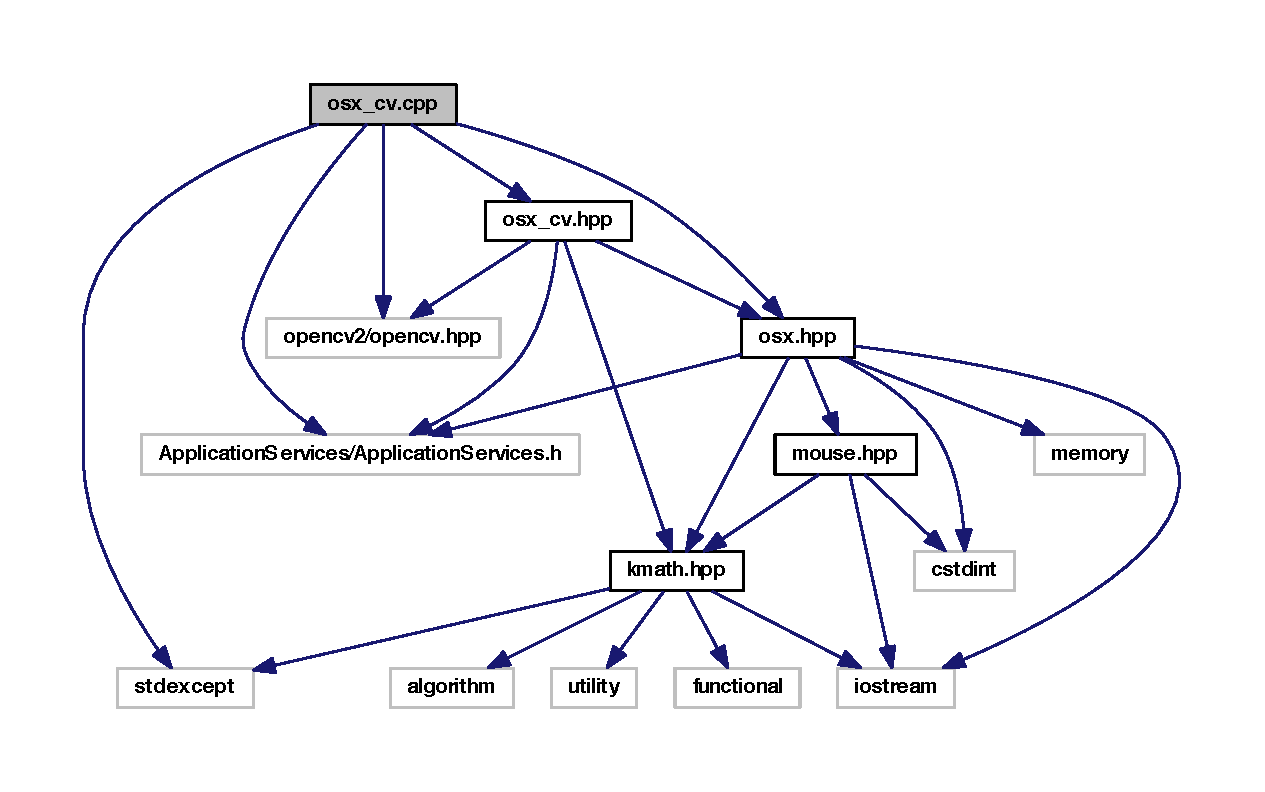
\includegraphics[width=350pt]{osx__cv_8cpp__incl}
\end{center}
\end{figure}

\hypertarget{osx__cv_8hpp}{\section{osx\-\_\-cv.\-hpp File Reference}
\label{osx__cv_8hpp}\index{osx\-\_\-cv.\-hpp@{osx\-\_\-cv.\-hpp}}
}
{\ttfamily \#include $<$opencv2/opencv.\-hpp$>$}\\*
{\ttfamily \#include $<$Application\-Services/\-Application\-Services.\-h$>$}\\*
{\ttfamily \#include \char`\"{}osx.\-hpp\char`\"{}}\\*
{\ttfamily \#include \char`\"{}kmath.\-hpp\char`\"{}}\\*
Include dependency graph for osx\-\_\-cv.\-hpp\-:
\nopagebreak
\begin{figure}[H]
\begin{center}
\leavevmode
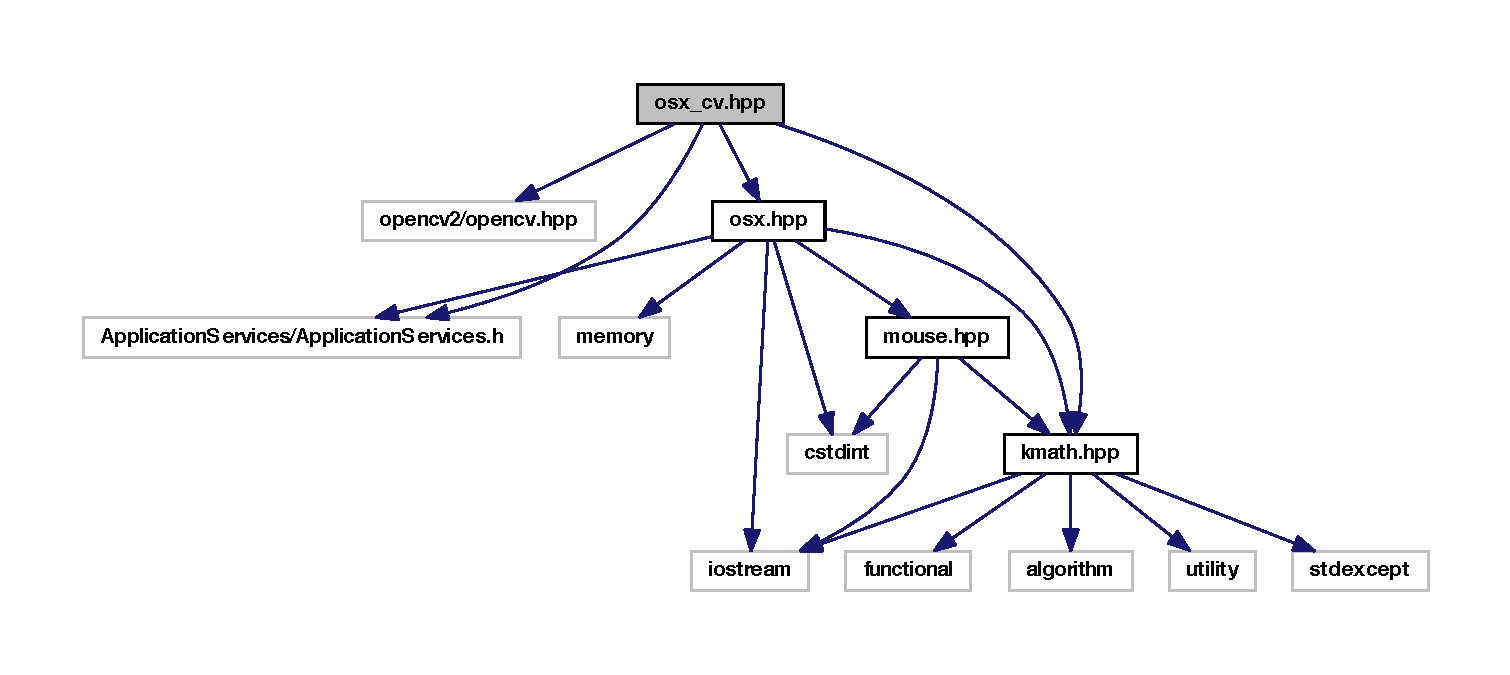
\includegraphics[width=350pt]{osx__cv_8hpp__incl}
\end{center}
\end{figure}
This graph shows which files directly or indirectly include this file\-:\nopagebreak
\begin{figure}[H]
\begin{center}
\leavevmode
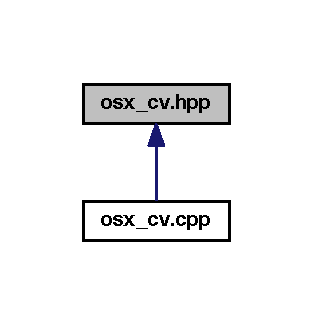
\includegraphics[width=150pt]{osx__cv_8hpp__dep__incl}
\end{center}
\end{figure}
\subsection*{Namespaces}
\begin{DoxyCompactItemize}
\item 
namespace \hyperlink{namespaceosx__cv}{osx\-\_\-cv}
\begin{DoxyCompactList}\small\item\em Functions for interoperability between Application\-Services and Open\-C\-V. \end{DoxyCompactList}\end{DoxyCompactItemize}
\subsection*{Functions}
\begin{DoxyCompactItemize}
\item 
cv\-::\-Mat \& \hyperlink{namespaceosx__cv_a06ac26ae0cdd938ae2885095282aef15}{osx\-\_\-cv\-::to\-Mat} (const C\-G\-Image\-Ref \&image, cv\-::\-Mat \&out, \hyperlink{namespaceosx_1_1disp_a63adf9b0b0b0365ec428dd44fc30c659}{osx\-::disp\-::\-R\-G\-B\-Type} dest\-Type=\hyperlink{namespaceosx_1_1disp_a63adf9b0b0b0365ec428dd44fc30c659ab96ecb2ad3c69bf9019d7ed4253603b1}{osx\-::disp\-::\-C\-O\-L\-O\-R\-\_\-\-B\-G\-R})
\begin{DoxyCompactList}\small\item\em Convert a {\ttfamily C\-G\-Image\-Ref} to a {\ttfamily cv\-::\-Mat}. \end{DoxyCompactList}\item 
C\-G\-Point \hyperlink{namespaceosx__cv_a501b2a8c59949eb3d398e8a9b58372b4}{osx\-\_\-cv\-::to\-C\-G\-Pt} (cv\-::\-Point pt)
\begin{DoxyCompactList}\small\item\em Convert a {\ttfamily cv\-::\-Point} to a {\ttfamily C\-G\-Point}. \end{DoxyCompactList}\item 
cv\-::\-Point \hyperlink{namespaceosx__cv_a9a9f0fa8d7a16879c88a19914a3c2484}{osx\-\_\-cv\-::to\-C\-V\-Pt} (C\-G\-Point pt)
\begin{DoxyCompactList}\small\item\em Convert a {\ttfamily C\-G\-Point} to a {\ttfamily cv\-::\-Point}. \end{DoxyCompactList}\end{DoxyCompactItemize}

\hypertarget{seq_8hpp}{\section{seq.\-hpp File Reference}
\label{seq_8hpp}\index{seq.\-hpp@{seq.\-hpp}}
}
{\ttfamily \#include $<$cmath$>$}\\*
{\ttfamily \#include $<$cstddef$>$}\\*
{\ttfamily \#include $<$stdexcept$>$}\\*
{\ttfamily \#include $<$iostream$>$}\\*
{\ttfamily \#include $<$algorithm$>$}\\*
{\ttfamily \#include $<$iterator$>$}\\*
{\ttfamily \#include $<$utility$>$}\\*
{\ttfamily \#include \char`\"{}kmath.\-hpp\char`\"{}}\\*
Include dependency graph for seq.\-hpp\-:\nopagebreak
\begin{figure}[H]
\begin{center}
\leavevmode
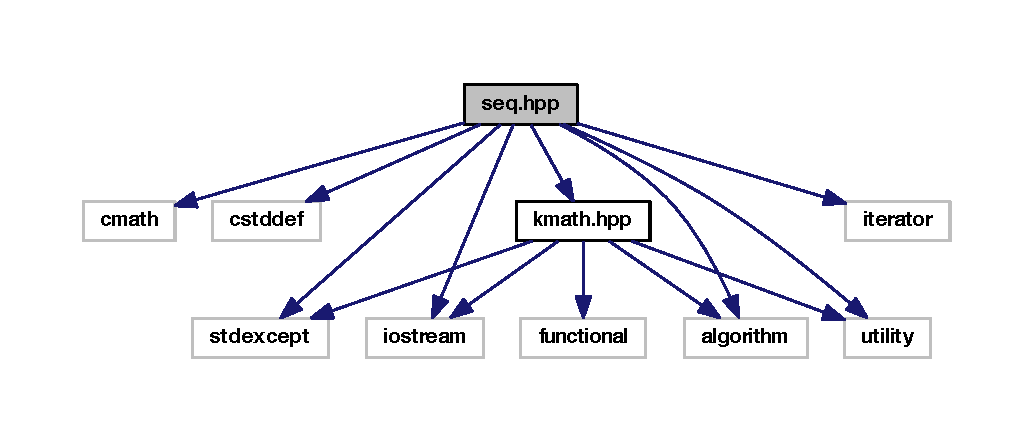
\includegraphics[width=350pt]{seq_8hpp__incl}
\end{center}
\end{figure}
This graph shows which files directly or indirectly include this file\-:\nopagebreak
\begin{figure}[H]
\begin{center}
\leavevmode
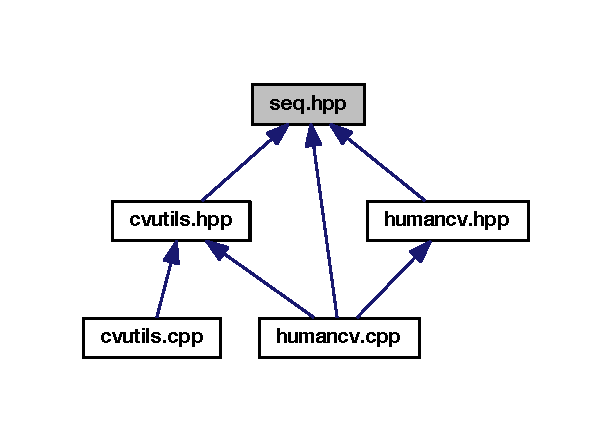
\includegraphics[width=243pt]{seq_8hpp__dep__incl}
\end{center}
\end{figure}
\subsection*{Classes}
\begin{DoxyCompactItemize}
\item 
struct \hyperlink{structseq_1_1_elem_view}{seq\-::\-Elem\-View$<$ Seq\-T $>$}
\begin{DoxyCompactList}\small\item\em Provides a reference and an index of an element in a sequence. \end{DoxyCompactList}\item 
struct \hyperlink{structseq_1_1_wrapped_seq}{seq\-::\-Wrapped\-Seq$<$ Seq\-T $>$}
\begin{DoxyCompactList}\small\item\em Sequence wrapper that supports wrap-\/around indexing -\/ all accessors will accept negative and out-\/of-\/bound indices and wrap around. \end{DoxyCompactList}\item 
class \hyperlink{classseq_1_1math_1_1_x_range_iterator}{seq\-::math\-::\-X\-Range\-Iterator$<$ Num\-T $>$}
\begin{DoxyCompactList}\small\item\em Lazy iterator used for X\-Range(), usually not necessary to use directly. \end{DoxyCompactList}\item 
struct \hyperlink{structseq_1_1math_1_1_x_range}{seq\-::math\-::\-X\-Range$<$ Num\-T $>$}
\begin{DoxyCompactList}\small\item\em Represent a lazily-\/evaluated range of numbers. \end{DoxyCompactList}\end{DoxyCompactItemize}
\subsection*{Namespaces}
\begin{DoxyCompactItemize}
\item 
namespace \hyperlink{namespaceseq}{seq}
\begin{DoxyCompactList}\small\item\em Generic sequence operations and structures. \end{DoxyCompactList}\item 
namespace \hyperlink{namespaceseq_1_1functional}{seq\-::functional}
\begin{DoxyCompactList}\small\item\em Functions commonly used in functional programming. \end{DoxyCompactList}\item 
namespace \hyperlink{namespaceseq_1_1math}{seq\-::math}
\begin{DoxyCompactList}\small\item\em Mathematical operations on sequences, and sequence structures. \end{DoxyCompactList}\end{DoxyCompactItemize}
\subsection*{Functions}
\begin{DoxyCompactItemize}
\item 
{\footnotesize template$<$class Seq\-T , typename Operand\-T $>$ }\\Seq\-T \& \hyperlink{seq_8hpp_a21a5aae4d520e12d3c987499aea2c0c4}{operator$\ast$=} (Seq\-T \&s, const Operand\-T \&e)
\begin{DoxyCompactList}\small\item\em Multiply each element in a sequence by {\ttfamily e}. \end{DoxyCompactList}\item 
{\footnotesize template$<$class Seq\-T , typename Operand\-T $>$ }\\Seq\-T \& \hyperlink{seq_8hpp_acf7f6f44050c057ff8e397070f2c497b}{operator/=} (Seq\-T \&s, const Operand\-T \&e)
\begin{DoxyCompactList}\small\item\em Divide each element in a sequence by {\ttfamily e}. \end{DoxyCompactList}\item 
size\-\_\-t \hyperlink{namespaceseq_a9f008982bf05fc256d4b035890744c77}{seq\-::\-\_\-real\-I} (int i, size\-\_\-t sz)
\begin{DoxyCompactList}\small\item\em Get the wrapped index to an array of size {\ttfamily sz}. \end{DoxyCompactList}\item 
size\-\_\-t \hyperlink{namespaceseq_ae4290a190db34f394330d88a5de8f2a7}{seq\-::\-\_\-real\-I\-Dist} (size\-\_\-t left\-I, size\-\_\-t right\-I, size\-\_\-t sz)
\begin{DoxyCompactList}\small\item\em Get the wrapped distance between left and right indices in an array of size {\ttfamily sz}. \end{DoxyCompactList}\item 
{\footnotesize template$<$class Seq\-T $>$ }\\Slice$<$ typename Seq\-T\-::iterator $>$ \hyperlink{namespaceseq_a01ecaea35db083541a258a05ac8c1d30}{seq\-::sl} (Seq\-T \&in, int i1, int i2)
\begin{DoxyCompactList}\small\item\em Get slice of sequence as a pair of iterators. \end{DoxyCompactList}\item 
{\footnotesize template$<$class In\-Seq\-T , class Out\-Seq\-T , typename \-\_\-\-Func\-T $>$ }\\Out\-Seq\-T \& \hyperlink{namespaceseq_1_1functional_ad36a538cd982a860de04e7f4af03bc4c}{seq\-::functional\-::map} (const \-\_\-\-Func\-T \&func, const In\-Seq\-T \&in, Out\-Seq\-T \&out)
\item 
{\footnotesize template$<$class In\-Seq\-T , class Out\-Seq\-T  = In\-Seq\-T, typename \-\_\-\-Func\-T $>$ }\\Out\-Seq\-T \hyperlink{namespaceseq_1_1functional_ab95c352080a36fe07cb04fe95b95caf8}{seq\-::functional\-::map} (const \-\_\-\-Func\-T \&func, const In\-Seq\-T \&in)
\item 
{\footnotesize template$<$class In\-Seq\-T , class Out\-Seq\-T , typename \-\_\-\-Func\-T $>$ }\\Out\-Seq\-T \& \hyperlink{namespaceseq_1_1functional_a5054f153ed880f89b744eec7aab118cf}{seq\-::functional\-::filter} (const \-\_\-\-Func\-T \&test, const In\-Seq\-T \&in, Out\-Seq\-T \&out)
\item 
{\footnotesize template$<$class In\-Seq\-T , class Out\-Seq\-T  = In\-Seq\-T, typename \-\_\-\-Func\-T $>$ }\\Out\-Seq\-T \hyperlink{namespaceseq_1_1functional_af3c889426da274197c74d0ec794072ff}{seq\-::functional\-::filter} (const \-\_\-\-Func\-T \&test, const In\-Seq\-T \&in)
\item 
{\footnotesize template$<$class Seq\-T , typename \-\_\-\-Func\-T $>$ }\\bool \hyperlink{namespaceseq_1_1functional_aadc273f6584110ccd147c612a2c315ab}{seq\-::functional\-::any} (const \-\_\-\-Func\-T \&test, const Seq\-T \&in)
\item 
{\footnotesize template$<$class Iter\-T , typename \-\_\-\-Func\-T $>$ }\\bool \hyperlink{namespaceseq_1_1functional_af131c7ae7d3ef6731a5e1fb71a8177aa}{seq\-::functional\-::any} (const \-\_\-\-Func\-T \&test, const Slice$<$ Iter\-T $>$ \&its)
\item 
{\footnotesize template$<$class Seq\-T , typename \-\_\-\-Func\-T $>$ }\\bool \hyperlink{namespaceseq_1_1functional_a2ffd96ef955260495f894c6eee90983c}{seq\-::functional\-::all} (const \-\_\-\-Func\-T \&test, const Seq\-T \&in)
\item 
{\footnotesize template$<$class Iter\-T , typename \-\_\-\-Func\-T $>$ }\\bool \hyperlink{namespaceseq_1_1functional_a6758cc8e1072ff3e3c0c32f121c879f4}{seq\-::functional\-::all} (const \-\_\-\-Func\-T \&test, const Slice$<$ Iter\-T $>$ \&its)
\item 
{\footnotesize template$<$typename Num\-T $>$ }\\X\-Range$<$ Num\-T $>$ \hyperlink{namespaceseq_1_1math_abfe793e999a374a4d5e6b1ef3f268b59}{seq\-::math\-::xrange} (Num\-T low, Num\-T high, Num\-T step=1, bool inclusive=false)
\begin{DoxyCompactList}\small\item\em Return {\ttfamily \hyperlink{structseq_1_1math_1_1_x_range}{X\-Range}} sequence, similar to Python's \char`\"{}xrange\char`\"{}. \end{DoxyCompactList}\item 
{\footnotesize template$<$typename Num\-T $>$ }\\X\-Range$<$ Num\-T $>$ \hyperlink{namespaceseq_1_1math_a4f2c47e50ba86a80778ccebd31d7fa16}{seq\-::math\-::xrange} (Num\-T high, bool inclusive=false)
\item 
{\footnotesize template$<$typename Num\-T , class Seq\-T $>$ }\\Seq\-T \& \hyperlink{namespaceseq_1_1math_a6bd86d848fb47f455aff84c38c175ea4}{seq\-::math\-::range} (Num\-T low, Num\-T high, Seq\-T \&out, Num\-T step=1)
\begin{DoxyCompactList}\small\item\em Construct a sequence of numbers from low to high with optional step. \end{DoxyCompactList}\item 
{\footnotesize template$<$typename Num\-T , class Seq\-T $>$ }\\Seq\-T \& \hyperlink{namespaceseq_1_1math_ae9b127e8277c6c390b99c4a1195dc087}{seq\-::math\-::range} (Num\-T high, Seq\-T \&out)
\begin{DoxyCompactList}\small\item\em Construct a sequence of numbers from 0 to high with step=1. \end{DoxyCompactList}\item 
{\footnotesize template$<$class Seq\-T $>$ }\\Seq\-T\-::value\-\_\-type \hyperlink{namespaceseq_1_1math_a27179daf6ca9a8d85434eda531fa134e}{seq\-::math\-::sum} (const Seq\-T \&in)
\begin{DoxyCompactList}\small\item\em Return the sum of sequence elements. \end{DoxyCompactList}\item 
{\footnotesize template$<$class Seq\-T $>$ }\\Seq\-T\-::value\-\_\-type \hyperlink{namespaceseq_1_1math_ab019165412bf99555adfeaaaa86f319f}{seq\-::math\-::mean} (const Seq\-T \&in)
\begin{DoxyCompactList}\small\item\em Return the arithmetic mean of sequence elements. \end{DoxyCompactList}\item 
{\footnotesize template$<$class Seq\-T $>$ }\\ostream \& \hyperlink{seq_8hpp_a25fc1874bf51d15a3fdfc0f63f75caa1}{operator$<$$<$} (ostream \&out, const \hyperlink{structseq_1_1_elem_view}{seq\-::\-Elem\-View}$<$ Seq\-T $>$ \&e)
\item 
{\footnotesize template$<$class Seq\-T $>$ }\\ostream \& \hyperlink{seq_8hpp_a987930fe6565e46853fbeb408ea3949b}{operator$<$$<$} (ostream \&out, const \hyperlink{structseq_1_1_wrapped_seq}{seq\-::\-Wrapped\-Seq}$<$ Seq\-T $>$ \&s)
\item 
{\footnotesize template$<$typename Elem\-Type , template$<$ typename U, class Alloc=allocator$<$ U $>$$>$ class Seq\-Type$>$ }\\ostream \& \hyperlink{seq_8hpp_a29425033946ee1e964e62754a6de891d}{operator$<$$<$} (ostream \&out, const Seq\-Type$<$ Elem\-Type $>$ \&seq)
\begin{DoxyCompactList}\small\item\em Print each element of a container, surrounded by {\ttfamily \mbox{[}\mbox{]}} and separated by commas. \end{DoxyCompactList}\end{DoxyCompactItemize}


\subsection{Function Documentation}
\hypertarget{seq_8hpp_a21a5aae4d520e12d3c987499aea2c0c4}{\index{seq.\-hpp@{seq.\-hpp}!operator$\ast$=@{operator$\ast$=}}
\index{operator$\ast$=@{operator$\ast$=}!seq.hpp@{seq.\-hpp}}
\subsubsection[{operator$\ast$=}]{\setlength{\rightskip}{0pt plus 5cm}template$<$class Seq\-T , typename Operand\-T $>$ Seq\-T\& operator$\ast$= (
\begin{DoxyParamCaption}
\item[{Seq\-T \&}]{s, }
\item[{const Operand\-T \&}]{e}
\end{DoxyParamCaption}
)}}\label{seq_8hpp_a21a5aae4d520e12d3c987499aea2c0c4}


Multiply each element in a sequence by {\ttfamily e}. 

\hypertarget{seq_8hpp_acf7f6f44050c057ff8e397070f2c497b}{\index{seq.\-hpp@{seq.\-hpp}!operator/=@{operator/=}}
\index{operator/=@{operator/=}!seq.hpp@{seq.\-hpp}}
\subsubsection[{operator/=}]{\setlength{\rightskip}{0pt plus 5cm}template$<$class Seq\-T , typename Operand\-T $>$ Seq\-T\& operator/= (
\begin{DoxyParamCaption}
\item[{Seq\-T \&}]{s, }
\item[{const Operand\-T \&}]{e}
\end{DoxyParamCaption}
)}}\label{seq_8hpp_acf7f6f44050c057ff8e397070f2c497b}


Divide each element in a sequence by {\ttfamily e}. 

\hypertarget{seq_8hpp_a25fc1874bf51d15a3fdfc0f63f75caa1}{\index{seq.\-hpp@{seq.\-hpp}!operator$<$$<$@{operator$<$$<$}}
\index{operator$<$$<$@{operator$<$$<$}!seq.hpp@{seq.\-hpp}}
\subsubsection[{operator$<$$<$}]{\setlength{\rightskip}{0pt plus 5cm}template$<$class Seq\-T $>$ ostream\& operator$<$$<$ (
\begin{DoxyParamCaption}
\item[{ostream \&}]{out, }
\item[{const {\bf seq\-::\-Elem\-View}$<$ Seq\-T $>$ \&}]{e}
\end{DoxyParamCaption}
)}}\label{seq_8hpp_a25fc1874bf51d15a3fdfc0f63f75caa1}
\hypertarget{seq_8hpp_a987930fe6565e46853fbeb408ea3949b}{\index{seq.\-hpp@{seq.\-hpp}!operator$<$$<$@{operator$<$$<$}}
\index{operator$<$$<$@{operator$<$$<$}!seq.hpp@{seq.\-hpp}}
\subsubsection[{operator$<$$<$}]{\setlength{\rightskip}{0pt plus 5cm}template$<$class Seq\-T $>$ ostream\& operator$<$$<$ (
\begin{DoxyParamCaption}
\item[{ostream \&}]{out, }
\item[{const {\bf seq\-::\-Wrapped\-Seq}$<$ Seq\-T $>$ \&}]{s}
\end{DoxyParamCaption}
)}}\label{seq_8hpp_a987930fe6565e46853fbeb408ea3949b}
\hypertarget{seq_8hpp_a29425033946ee1e964e62754a6de891d}{\index{seq.\-hpp@{seq.\-hpp}!operator$<$$<$@{operator$<$$<$}}
\index{operator$<$$<$@{operator$<$$<$}!seq.hpp@{seq.\-hpp}}
\subsubsection[{operator$<$$<$}]{\setlength{\rightskip}{0pt plus 5cm}template$<$typename Elem\-Type , template$<$ typename U, class Alloc=allocator$<$ U $>$$>$ class Seq\-Type$>$ ostream\& operator$<$$<$ (
\begin{DoxyParamCaption}
\item[{ostream \&}]{out, }
\item[{const Seq\-Type$<$ Elem\-Type $>$ \&}]{seq}
\end{DoxyParamCaption}
)}}\label{seq_8hpp_a29425033946ee1e964e62754a6de891d}


Print each element of a container, surrounded by {\ttfamily \mbox{[}\mbox{]}} and separated by commas. 


\hypertarget{str_8cpp}{\section{str.\-cpp File Reference}
\label{str_8cpp}\index{str.\-cpp@{str.\-cpp}}
}
{\ttfamily \#include $<$string$>$}\\*
{\ttfamily \#include $<$stdexcept$>$}\\*
{\ttfamily \#include \char`\"{}str.\-hpp\char`\"{}}\\*
{\ttfamily \#include \char`\"{}io.\-hpp\char`\"{}}\\*
Include dependency graph for str.\-cpp\-:\nopagebreak
\begin{figure}[H]
\begin{center}
\leavevmode
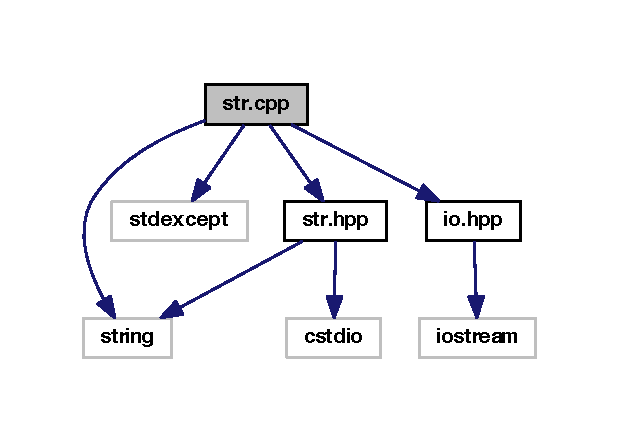
\includegraphics[width=297pt]{str_8cpp__incl}
\end{center}
\end{figure}

\hypertarget{str_8hpp}{\section{str.\-hpp File Reference}
\label{str_8hpp}\index{str.\-hpp@{str.\-hpp}}
}
{\ttfamily \#include $<$cstdio$>$}\\*
{\ttfamily \#include $<$string$>$}\\*
\subsection*{Namespaces}
\begin{DoxyCompactItemize}
\item 
namespace \hyperlink{namespacestr}{str}
\begin{DoxyCompactList}\small\item\em String utilities. \end{DoxyCompactList}\end{DoxyCompactItemize}
\subsection*{Defines}
\begin{DoxyCompactItemize}
\item 
\#define \hyperlink{str_8hpp_ad02d698209df17aef336d5633065c5ab}{str\-Fmt}(fmt,...)~(snprintf(\hyperlink{namespacestr_a51a7257ade189ec55f5d1c9da0f0e8b4}{str\-::\-\_\-buf}, 100, fmt, \-\_\-\-\_\-\-V\-A\-\_\-\-A\-R\-G\-S\-\_\-\-\_\-), \hyperlink{namespacestr_a51a7257ade189ec55f5d1c9da0f0e8b4}{str\-::\-\_\-buf})
\end{DoxyCompactItemize}
\subsection*{Functions}
\begin{DoxyCompactItemize}
\item 
string \hyperlink{namespacestr_a7b677ee9cce42c91dcd37d68b7fa04ac}{str\-::word\-Wrap} (string in, unsigned cols=80)  throw (length\-\_\-error)
\end{DoxyCompactItemize}
\subsection*{Variables}
\begin{DoxyCompactItemize}
\item 
char \hyperlink{namespacestr_a51a7257ade189ec55f5d1c9da0f0e8b4}{str\-::\-\_\-buf} \mbox{[}100\mbox{]}
\end{DoxyCompactItemize}


\subsection{Define Documentation}
\hypertarget{str_8hpp_ad02d698209df17aef336d5633065c5ab}{\index{str.\-hpp@{str.\-hpp}!str\-Fmt@{str\-Fmt}}
\index{str\-Fmt@{str\-Fmt}!str.hpp@{str.\-hpp}}
\subsubsection[{str\-Fmt}]{\setlength{\rightskip}{0pt plus 5cm}\#define {\bf str\-Fmt}(
\begin{DoxyParamCaption}
\item[{}]{fmt, }
\item[{}]{...}
\end{DoxyParamCaption}
)~(snprintf({\bf str\-::\-\_\-buf}, 100, fmt, \-\_\-\-\_\-\-V\-A\-\_\-\-A\-R\-G\-S\-\_\-\-\_\-), {\bf str\-::\-\_\-buf})}}\label{str_8hpp_ad02d698209df17aef336d5633065c5ab}
Functional version of {\ttfamily snprintf}.

Yes, macros are evil, but this is so convenient. 
\hypertarget{thr_8hpp}{\section{thr.\-hpp File Reference}
\label{thr_8hpp}\index{thr.\-hpp@{thr.\-hpp}}
}
{\ttfamily \#include $<$deque$>$}\\*
{\ttfamily \#include $<$mutex$>$}\\*
Include dependency graph for thr.\-hpp\-:
\nopagebreak
\begin{figure}[H]
\begin{center}
\leavevmode
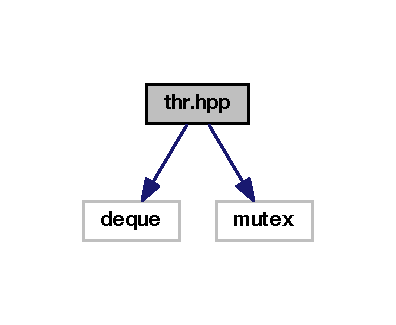
\includegraphics[width=190pt]{thr_8hpp__incl}
\end{center}
\end{figure}
\subsection*{Classes}
\begin{DoxyCompactItemize}
\item 
struct \hyperlink{structthr_1_1_queue}{thr\-::\-Queue$<$ T $>$}
\begin{DoxyCompactList}\small\item\em Producer-\/consumer queue. \end{DoxyCompactList}\end{DoxyCompactItemize}
\subsection*{Namespaces}
\begin{DoxyCompactItemize}
\item 
namespace \hyperlink{namespacethr}{thr}
\begin{DoxyCompactList}\small\item\em Multi-\/threading utilities. \end{DoxyCompactList}\end{DoxyCompactItemize}

\printindex
\end{document}
